\documentclass[oneside, 12pt]{report}

\usepackage[a4paper, left=3cm, right=3cm, top=4cm, bottom=3cm]{geometry}
\usepackage{iftex}
\ifPDFTeX
  \usepackage[T1]{fontenc}
  \usepackage[utf8]{inputenc}
\else
  \usepackage{fontspec}
  \defaultfontfeatures{Scale=MatchLowercase}
\fi
\usepackage[italian]{babel}
\usepackage{graphicx}
\graphicspath{{figure/}}
\usepackage{url}
\usepackage{subfig}
\usepackage{amsmath, amssymb, amsfonts}
\ifPDFTeX\else
  \usepackage{unicode-math}
\fi
\usepackage{newunicodechar}
  \newunicodechar{±}{\ensuremath{\pm}}
  \newunicodechar{·}{\ensuremath{\cdot}}
  \newunicodechar{×}{\ensuremath{\times}}
  \newunicodechar{ʳ}{\ensuremath{{}^{r}}}
  \newunicodechar{Δ}{\ensuremath{\Delta}}
  \newunicodechar{Σ}{\ensuremath{\Sigma}}
  \newunicodechar{α}{\ensuremath{\alpha}}
  \newunicodechar{β}{\ensuremath{\beta}}
  \newunicodechar{γ}{\ensuremath{\gamma}}
  \newunicodechar{λ}{\ensuremath{\lambda}}
  \newunicodechar{μ}{\ensuremath{\mu}}
  \newunicodechar{π}{\ensuremath{\pi}}
  \newunicodechar{ρ}{\ensuremath{\rho}}
  \newunicodechar{τ}{\ensuremath{\tau}}
  \newunicodechar{φ}{\ensuremath{\varphi}}
  \newunicodechar{ψ}{\ensuremath{\psi}}
  \newunicodechar{ᵐ}{\ensuremath{{}^{m}}}
  \newunicodechar{ᵢ}{\ensuremath{{}_{i}}}
  \newunicodechar{†}{\ensuremath{\dagger}}
  \newunicodechar{⁰}{\ensuremath{{}^{0}}}
  \newunicodechar{¹}{\ensuremath{{}^{1}}}
  \newunicodechar{²}{\ensuremath{{}^{2}}}
  \newunicodechar{³}{\ensuremath{{}^{3}}}
  \newunicodechar{⁴}{\ensuremath{{}^{4}}}
  \newunicodechar{⁵}{\ensuremath{{}^{5}}}
  \newunicodechar{⁶}{\ensuremath{{}^{6}}}
  \newunicodechar{⁷}{\ensuremath{{}^{7}}}
  \newunicodechar{⁸}{\ensuremath{{}^{8}}}
  \newunicodechar{⁹}{\ensuremath{{}^{9}}}
  \newunicodechar{⁻}{\ensuremath{{}^{-}}}
  \newunicodechar{₀}{\ensuremath{{}_{0}}}
  \newunicodechar{₁}{\ensuremath{{}_{1}}}
  \newunicodechar{₂}{\ensuremath{{}_{2}}}
  \newunicodechar{₌}{\ensuremath{{}_{=}}}
  \newunicodechar{ₖ}{\ensuremath{{}_{k}}}
  \newunicodechar{ₘ}{\ensuremath{{}_{m}}}
  \newunicodechar{→}{\ensuremath{\to}}
  \newunicodechar{∈}{\ensuremath{\in}}
  \newunicodechar{√}{\ensuremath{\sqrt{}}}
  \newunicodechar{∝}{\ensuremath{\propto}}
  \newunicodechar{≃}{\ensuremath{\simeq}}
  \newunicodechar{≈}{\ensuremath{\approx}}
  \newunicodechar{≡}{\ensuremath{\equiv}}
  \newunicodechar{≤}{\ensuremath{\leq}}
  \newunicodechar{≥}{\ensuremath{\geq}}
  \newunicodechar{⌈}{\ensuremath{\lceil}}
  \newunicodechar{⌉}{\ensuremath{\rceil}}
  \newunicodechar{⌊}{\ensuremath{\lfloor}}
  \newunicodechar{⌋}{\ensuremath{\rfloor}}
  \newunicodechar{⟨}{\ensuremath{\langle}}
  \newunicodechar{⟩}{\ensuremath{\rangle}}
  \newunicodechar{✓}{\ensuremath{\checkmark}}
\usepackage{braket}         %
\usepackage{textcomp}
\usepackage{xcolor}
\usepackage{afterpage}
\usepackage{bm}
\usepackage{multirow}
\usepackage{algorithm}
\usepackage{algpseudocode}
\usepackage{pgfplots}
\pgfplotsset{compat=1.18}
\usepackage{tikz}
\usetikzlibrary{quantikz2}  %
\usetikzlibrary{positioning, arrows.meta, calc}
\usetikzlibrary{decorations.pathmorphing, decorations.pathreplacing}  %
\usepackage{listings}
\usepackage{microtype}
\usepackage{csquotes}
\usepackage{pifont}
\renewcommand{\checkmark}{\ding{51}}
\usepackage{booktabs}
\usepackage{tabularx}
\usepackage{longtable}
\usepackage{array}
\usepackage{etoolbox}
\usepackage{needspace}  %
\AtBeginEnvironment{longtable}{\small\setstretch{1}\renewcommand{\arraystretch}{1.2}}
\AtBeginEnvironment{tabular}{\setstretch{1}\renewcommand{\arraystretch}{1.2}}
\AtBeginEnvironment{tabularx}{\setstretch{1}\renewcommand{\arraystretch}{1.2}}
\renewcommand{\tabularxcolumn}[1]{>{\raggedright\arraybackslash}p{#1}}
\usepackage{calc}
\usepackage{caption}
\captionsetup[table]{position=bottom,skip=8pt,font=small,labelfont=bf,justification=raggedright,singlelinecheck=false}
\captionsetup[figure]{position=bottom,skip=8pt,labelfont=bf,textfont=normalfont}
\newcounter{none}
\providecommand{\tightlist}{%
  \setlength{\itemsep}{0pt}\setlength{\parskip}{0pt}}
\usepackage{setspace}
\usepackage[bottom]{footmisc}
\usepackage{float}
\setcounter{topnumber}{3}
\setcounter{bottomnumber}{2}
\setcounter{totalnumber}{5}
\renewcommand{\topfraction}{0.90}
\renewcommand{\bottomfraction}{0.80}
\renewcommand{\textfraction}{0.08}
\renewcommand{\floatpagefraction}{0.75}
\setlength{\emergencystretch}{3em}
\usepackage[backend=biber, citestyle=numeric, sorting=none]{biblatex}
\usepackage[breaklinks, hidelinks]{hyperref}
\usepackage[acronym, nopostdot, nogroupskip, toc]{glossaries}
\makenoidxglossaries
\let\ac\gls
\providecommand{\acf}[1]{\acrfull{#1}}
\providecommand{\acl}[1]{\acrlong{#1}}
\providecommand{\acs}[1]{\acrshort{#1}}
\newacronym{BHT}{BHT}{Brassard-H\o yer-Tapp}
\newacronym{BQP}{BQP}{\textit{Bounded-error Quantum Polynomial time}}
\newacronym{CCNOT}{CCNOT}{Controlled-Controlled NOT (porta di Toffoli)}
\newacronym{CDR}{CDR}{\textit{Clifford Data Regression}}
\newacronym{CNF}{CNF}{Forma Normale Congiuntiva (\textit{Conjunctive Normal Form})}
\newacronym{CNOT}{CNOT}{Controlled-NOT}
\newacronym{CPTP}{CPTP}{\textit{Completely Positive Trace-Preserving}}
\newacronym{DFT}{DFT}{Trasformata Discreta di Fourier (\textit{Discrete Fourier Transform})}
\newacronym{DSA}{DSA}{\textit{Digital Signature Algorithm}}
\newacronym{ECDSA}{ECDSA}{\textit{Elliptic Curve Digital Signature Algorithm}}
\newacronym{GNFS}{GNFS}{\textit{General Number Field Sieve}}
\newacronym{HTTPS}{HTTPS}{\textit{HyperText Transfer Protocol Secure}}
\newacronym{IBM}{IBM}{International Business Machines}
\newacronym{MIT}{MIT}{Massachusetts Institute of Technology}
\newacronym{NIST}{NIST}{\textit{National Institute of Standards and Technology}}
\newacronym{NISQ}{NISQ}{\textit{Noisy Intermediate-Scale Quantum}}
\newacronym{NMR}{NMR}{Risonanza Magnetica Nucleare (\textit{Nuclear Magnetic Resonance})}
\newacronym{PEC}{PEC}{\textit{Probabilistic Error Cancellation}}
\newacronym{FFT}{FFT}{Trasformata Rapida di Fourier (\textit{Fast Fourier Transform})}
\newacronym{PQC}{PQC}{\textit{Post-Quantum Cryptography}}
\newacronym{QEC}{QEC}{Correzione degli Errori Quantistici (\textit{Quantum Error Correction})}
\newacronym{QFT}{QFT}{Trasformata di Fourier Quantistica (\textit{Quantum Fourier Transform})}
\newacronym{AQFT}{AQFT}{Trasformata di Fourier Quantistica Approssimata (\textit{Approximate Quantum Fourier Transform})}
\newacronym{QML}{QML}{\textit{Quantum Machine Learning}}
\newacronym{QMA}{QMA}{\textit{Quantum Merlin-Arthur}}
\newacronym{QPE}{QPE}{\textit{Quantum Phase Estimation}}
\newacronym{RSA}{RSA}{Rivest-Shamir-Adleman}
\newacronym{SAT}{SAT}{Soddisfacibilità Booleana (\textit{Boolean Satisfiability})}
\newacronym{SSH}{SSH}{\textit{Secure Shell}}
\newacronym{TLS}{TLS}{\textit{Transport Layer Security}}
\newacronym{TSP}{TSP}{Problema del Commesso Viaggiatore (\textit{Travelling Salesman Problem})}
\newacronym{ZNE}{ZNE}{\textit{Zero-Noise Extrapolation}}
\newacronym{AUC}{AUC}{Area Sotto la Curva ROC (\textit{Area Under the Curve})}
\newacronym{ML}{ML}{Apprendimento Automatico (\textit{Machine Learning})}
\newacronym{LSTM}{LSTM}{\textit{Long Short-Term Memory}}
\newacronym{GCD}{GCD}{Massimo Comune Divisore (\textit{Greatest Common Divisor})}
\newacronym{GPU}{GPU}{Unità di Elaborazione Grafica (\textit{Graphics Processing Unit})}
\newacronym{MLP}{MLP}{Percettrone Multistrato (\textit{Multi-Layer Perceptron})}
\newacronym{SVM}{SVM}{\textit{Support Vector Machine}}
\newacronym{WSL}{WSL}{\textit{Windows Subsystem for Linux}}
\newacronym{SDK}{SDK}{\textit{Software Development Kit}}
\newacronym{API}{API}{\textit{Application Programming Interface}}
\newacronym{CPU}{CPU}{Unità di Elaborazione Centrale (\textit{Central Processing Unit})}
\newacronym{CX}{CX}{Controlled-X (porta CNOT)}
\newacronym{QPU}{QPU}{Unità di Elaborazione Quantistica (\textit{Quantum Processing Unit})}
\newacronym{QAOA}{QAOA}{\textit{Quantum Approximate Optimization Algorithm}}
\newacronym{MWPM}{MWPM}{\textit{Minimum Weight Perfect Matching}}
\newacronym{CSS}{CSS}{Calderbank-Shor-Steane}
\newacronym{DEM}{DEM}{\textit{Detector Error Model}}
\newacronym{BPOSD}{BP+OSD}{\textit{Belief Propagation with Ordered Statistics Decoding}}
\newacronym{ECR}{ECR}{\textit{Echoed Cross-Resonance}}
\newacronym{IC}{IC}{Intervallo di Confidenza}
   %

\renewcommand{\lstlistingname}{Listato}
\renewcommand{\lstlistlistingname}{Elenco dei listati}

\lstset{
    language=Python,
    basicstyle=\ttfamily\small,
    keywordstyle=\color{blue}\bfseries,
    commentstyle=\color{gray}\itshape,
    stringstyle=\color{orange},
    showstringspaces=false,
    frame=none,
    breaklines=true,
    captionpos=b
}

\newcommand{\blankpage}{%
    \null\thispagestyle{empty}\addtocounter{page}{-1}\newpage
}

\newif\ifdecoderbody
\decoderbodyfalse

\onehalfspacing
\setlength{\skip\footins}{1cm}
\addbibresource{Bibliografia.bib}

\begin{document}

\hypersetup{pageanchor=false}
\begin{titlepage}
\thispagestyle{empty}

\begin{tikzpicture}[remember picture, overlay,
    centro/.style={inner sep=0pt, anchor=base},
    sinistra/.style={inner sep=0pt, anchor=base west},
    garamond/.style={font=\fontfamily{EBGaramond-TLF}\fontseries{b}%
        \fontshape{n}\fontsize{#1}{#1}\selectfont},
    garamond corsivo/.style={font=\fontfamily{EBGaramond-TLF}\fontseries{b}%
        \fontshape{it}\fontsize{#1}{#1}\selectfont},
    garamond nome/.style={font=\fontfamily{EBGaramond-TLF}\fontseries{m}%
        \fontshape{it}\fontsize{#1}{#1}\selectfont},
    palatino/.style={font=\usefont{T1}{ppl}{b}{n}\fontsize{#1}{#1}\selectfont},
    palatino nome/.style={font=\usefont{T1}{ppl}{m}{it}\fontsize{#1}{#1}\selectfont}]

    \node[sinistra, palatino=10]
        at ([shift={(30mm,-28.7mm)}]current page.north west)
        {Matr. N INLM03/23286};

    \node[inner sep=0pt, anchor=north]
        at ([yshift=-35.4mm]current page.north)
        {
\includegraphics[width=30.15mm]{figure/ucbm-logo.png}};

    \node[centro, garamond=16] at ([yshift=-74.3mm]current page.north)
        {UNIVERSIT\`A};
    \node[centro, garamond=16] at ([yshift=-83.8mm]current page.north)
        {CAMPUS BIO-MEDICO DI ROMA};

    \node[centro, garamond=14] at ([yshift=-112.4mm]current page.north)
        {FACOLT\`A DIPARTIMENTALE DI INGEGNERIA};
    \node[centro, garamond=14] at ([yshift=-118.1mm]current page.north)
        {CORSO DI LAUREA MAGISTRALE IN};
    \node[centro, garamond=14] at ([yshift=-123.6mm]current page.north)
        {INGEGNERIA DEI SISTEMI INTELLIGENTI};

    \node[centro, garamond=18] at ([yshift=-151.1mm]current page.north)
        {SHOR'S ALGORITHM UNDER NOISE:};
    \node[centro, garamond=18] at ([yshift=-158.2mm]current page.north)
        {MACHINE-LEARNING ABLATION,};
    \node[centro, garamond=18] at ([yshift=-165.4mm]current page.north)
        {QUANTUM ERROR CORRECTION,};
    \node[centro, garamond=18] at ([yshift=-172.5mm]current page.north)
        {AND APPROXIMATE QFT};

    \node[sinistra, garamond corsivo=14]
        at ([shift={(30mm,-194.2mm)}]current page.north west) {Relatore};
    \node[sinistra, palatino nome=12]
        at ([shift={(30mm,-199.9mm)}]current page.north west) {Prof. Paolo Soda};
    \node[sinistra, garamond corsivo=14]
        at ([shift={(30mm,-224.4mm)}]current page.north west) {Correlatore};
    \node[sinistra, palatino nome=12]
        at ([shift={(30mm,-230.4mm)}]current page.north west) {Prof. Floriano Caprio};

    \node[sinistra, garamond corsivo=14]
        at ([shift={(142.4mm,-240.5mm)}]current page.north west) {Laureando};
    \node[sinistra, garamond nome=12]
        at ([shift={(142.4mm,-245.6mm)}]current page.north west) {Claudio Dragotta};

    \node[centro, garamond=12] at ([yshift=-275.7mm]current page.north)
        {ANNO ACCADEMICO 2025/2026};
\end{tikzpicture}

\null
\afterpage{\blankpage}
\end{titlepage}


\ifdefined\copiarelatore\else
\begin{titlepage}
    \vspace*{5cm}
    \begin{flushright}
        \itshape
        Alla mia famiglia,\\
        che ha creduto in me\\
        quando io stesso dubitavo,\\
        e mi ha insegnato che la luce\\
        si trova anche camminando nel buio.

        \bigskip
        A me stesso,\\
        perché ho imparato che resistere\\
        non è l'assenza di paura,\\
        ma scegliere di restare\\
        quando nessuno ci credeva più.
    \end{flushright}
\end{titlepage}
\fi

\hypersetup{pageanchor=true}
\pagenumbering{roman}

\tableofcontents

\addcontentsline{toc}{chapter}{\listfigurename}
\listoffigures

\addcontentsline{toc}{chapter}{\listtablename}
\listoftables

\glsadd{ECR}\glsadd{IC}\glsadd{ML}\glsadd{RSA}
\printnoidxglossary[type=\acronymtype, nonumberlist, title={Elenco degli Acronimi}]

\clearpage
\pagenumbering{arabic}
\nocite{shor1994,buhler1993gnfs,rsa1978,preskill2018,skosana2021,yang2026,smolin2013,nielsenChuang2000,temme2017,steane1996,fowler2012,qiskit2023,stim2021,pymatching2021,scikit_learn,beauregard2002,googleQECBelowThreshold2025,alphaqubit2024,chevignard2025,wootters1982,shorcorrection1995,googleSurfaceCode2023,torlaiMelko2017,yan2026,roffe2020,panteleev2021,sarovar2020,barencoAQFT1996,akoramurthy2026,gidney2021,aharonov1997fault,dennis2002topological,kitaev2003,liBenjamin2017,rsa250_2020,shuklaqpe2026,shukla2026,zurek2003,vandersypen2001,monz2016,calderbankShor1996,gottesman1997,murali2019,tannu2019}

\chapter{Introduzione}
\label{chap:introduzione}

% Generato dalla versione Word revisionata e dalla bozza auditata.
% Le citazioni numeriche originali sono state convertite in chiavi BibLaTeX.

\section{Dal vantaggio teorico al problema del rumore}\label{sec:finale_1_1}

La fattorizzazione di grandi numeri interi è un esempio di problema per il quale l'aumento della potenza di calcolo classica non modifica la natura della difficoltà computazionale: il miglior algoritmo classico generale noto, il General Number Field Sieve, ha complessità sub-esponenziale ma non polinomiale nella lunghezza dell'input \cite{buhler1993gnfs,rsa250_2020}. Nel 1994 Peter Shor ha mostrato che, nel modello ideale di calcolo quantistico, la fattorizzazione e il logaritmo discreto possono invece essere risolti in tempo polinomiale \cite{shor1994}. Il risultato ha una conseguenza immediata per la sicurezza informatica, perché sistemi a chiave pubblica come RSA fondano la propria sicurezza pratica proprio sulla difficoltà di fattorizzare interi di grandi dimensioni \cite{rsa1978}.

Il vantaggio algoritmico, tuttavia, non coincide con la possibilità di eseguire oggi Shor su istanze crittograficamente rilevanti. I processori quantistici disponibili operano in un regime nel quale errori di gate, decoerenza, readout imperfetto, connettività limitata e crosstalk riducono la profondità dei circuiti eseguibili con affidabilità \cite{preskill2018}. Shor è particolarmente sensibile a questi effetti: la ricerca del periodo richiede di preservare informazione di fase lungo l'esponenziazione modulare e di renderla osservabile attraverso la Quantum Phase Estimation (QPE) e la Quantum Fourier Transform (QFT). Se il rumore disperde la probabilità che dovrebbe concentrarsi intorno agli esiti legati al periodo, la successiva elaborazione classica può non ricostruire i fattori corretti. Studi recenti su order finding rumoroso mostrano inoltre che la recoverability dipende dalla struttura residua della distribuzione e non dalla sola presenza visiva dei picchi \cite{skosana2021,yang2026,smolin2013}. Dimostrazioni sperimentali su piccole istanze hanno inoltre mostrato che i blocchi essenziali di Shor possono essere realizzati su piattaforme fisiche molto diverse, dalla NMR agli ioni intrappolati \cite{vandersypen2001,monz2016}; tali prove restano però lontane da una fattorizzazione fault-tolerant su scala crittografica \cite{smolin2013,gidney2021}.

Questa distanza tra vantaggio teorico e realizzabilità costituisce il punto di partenza della tesi. L'obiettivo non è individuare una tecnica ``migliore'' in assoluto, ma misurare come una specifica implementazione di Shor degradi al crescere di un proxy di errore per gate e valutare, con baseline esplicite, tre livelli di intervento: sfruttare meglio l'informazione residua nelle misure; proteggere l'informazione durante il calcolo; ridurre il numero di operazioni esposte al rumore. Il criterio guida è distinguere un miglioramento della metrica di interesse da un semplice aumento della complessità del metodo.

\section{Obiettivi e contributo del lavoro}\label{sec:finale_1_2}

Il lavoro adotta un principio metodologico comune a tutte le campagne: ogni tecnica viene confrontata con una baseline esplicita, sugli stessi dati quando il confronto lo consente, e mediante metriche coerenti con il compito osservato. Questa scelta è centrale perché, in presenza di rumore, un risultato apparentemente positivo può dipendere dal post-processing, dalla struttura particolare dell'istanza o da una metrica intermedia che non coincide con l'obiettivo finale. Tutti gli esperimenti della tesi sono simulativi; non vengono quindi presentati come una dimostrazione di fattibilità su hardware quantistico reale né come una previsione delle risorse necessarie per fattorizzare moduli di dimensione crittografica.

La prima linea di ricerca riguarda il post-processing degli output rumorosi di Shor. Sull'istanza principale N = 15, a = 7, vengono confrontate tre strategie applicate agli stessi istogrammi: TOP-1, che verifica il solo esito più frequente; TOP-4, che verifica i quattro candidati più frequenti; e un metodo che usa un classificatore di machine learning per decidere quando attivare la stessa ricerca TOP-4. Il confronto tra il metodo appreso e TOP-4 senza filtro costituisce l'ablazione del classificatore. La SVM selezionata raggiunge elevati valori delle metriche predittive, ma non riduce il numero di iterazioni necessarie alla fattorizzazione rispetto alla baseline; TOP-4, invece, raggiunge il successo alla prima iterazione in tutte le repliche dei due scenari principali. L'ablazione attribuisce quindi il beneficio alla ricerca multi-candidato, non al filtro appreso. Un confronto con la Zero-Noise Extrapolation (ZNE) completa la valutazione delle strategie a valle dell'esecuzione.

La seconda linea studia la Quantum Error Correction (QEC), cioè la protezione dell'informazione mentre il calcolo è in corso. Il percorso parte dal codice a ripetizione, prosegue con il codice di Steane \ensuremath{[[7,1,3]]} e arriva al surface code \cite{steane1996,fowler2012,googleQECBelowThreshold2025,googleSurfaceCode2023}. Nei circuiti di memoria viene misurato il tasso di errore logico al variare dell'errore fisico e, per il surface code, della distanza del codice. Le simulazioni riproducono la soppressione quadratica attesa per i codici a distanza tre e mostrano, nel surface code, il comportamento di soglia: sotto la soglia stimata aumentare la distanza riduce l'errore logico, mentre sopra soglia lo amplifica. Questi valori appartengono ai circuiti di memoria, al modello di rumore e ai decoder adottati e non vengono trasferiti direttamente alle porte logiche di Shor. Un confronto esplorativo nel modello code-capacity considera infine il Gross code di IBM, un codice quantum Low-Density Parity-Check (qLDPC) che protegge 12 qubit logici con 144 qubit di dato \cite{bravyi2024}: con un decoder adeguato protegge i 12 qubit logici meglio di 12 patch di surface code a distanza 13, che usano oltre quattordici volte i suoi qubit di dato, per errori fisici dallo 0,75\% in su, ma il vantaggio dipende in modo decisivo dalla configurazione del decoder.

All'interno della QEC viene inoltre studiato un secondo impiego del machine learning. Invece di classificare l'istogramma finale, la rete riceve la sindrome di errore. Quando il modello di rumore corrisponde alle assunzioni del decoder analitico, una rete usata come sostituto non mostra un vantaggio stabile rispetto al Minimum Weight Perfect Matching (MWPM). In presenza di correlazioni non ben rappresentate dal grafo del matching, una strategia ibrida può invece migliorare la decisione analitica correggendone alcuni errori residui. Il confronto successivo con BP+OSD mostra però che una parte del margine può dipendere dalla qualità del decoder di riferimento. Il risultato non è quindi una superiorità generale del machine learning, ma individua il regime nel quale un modello appreso può essere utile: quando osserva struttura informativa che il metodo analitico non rappresenta adeguatamente.

La terza linea interviene direttamente sulla complessità del circuito mediante una QFT approssimata (AQFT), che elimina rotazioni controllate di piccolo angolo. L'approssimazione riduce porte e profondità, ma introduce una perdita di precisione: il problema consiste quindi nel verificare se il rumore evitato compensi l'errore algoritmico aggiunto. Nel pilota su Shor con N = 15, il grado di troncamento scelto sui dati di selezione e valutato su dati indipendenti aumenta il successo da 0,4792 a 0,6279, mentre le porte ECR a due qubit scendono da 362 a 279. Il miglioramento è favorito dall'ordine r = 4, che produce fasi esattamente rappresentabili con due bit, e non viene generalizzato automaticamente a istanze differenti. Per N = 21 il troncamento dell'aritmetica riduce invece le porte a due qubit da 49 661 a 23 178, ma diminuisce il successo ideale e nei test rumorosi a budget ridotto non emerge un beneficio statisticamente dimostrato. Nei benchmark separati di QPE, al contrario, la variante troncata risulta migliore in tutti i nove confronti effettuati, con sei intervalli di confidenza individuali interamente positivi. Questi risultati mostrano che l'efficacia dell'AQFT dipende dal compromesso tra precisione di fase, costo circuitale e regime di rumore \cite{barencoAQFT1996,akoramurthy2026}.

L'analisi di sensibilità da cui parte lo studio applica un errore Pauli uniforme dopo le porte compilate: il successo per singola misura scende dal 74,89\% in assenza di errori fino a circa il 24,6\% ad alto rumore, valore che la sola verifica classica garantirebbe anche su esiti uniformi. Il parametro di questo esperimento è un proxy per gate e non coincide con il tasso di errore logico per round o per memoria misurato nelle campagne QEC. Mantenere separate queste grandezze evita una conclusione non supportata: la tesi non simula un'esecuzione end-to-end di Shor fault-tolerant, ma caratterizza separatamente la robustezza dell'algoritmo, la capacità dei codici di sopprimere gli errori e il comportamento dei decoder.

Nel complesso, il contributo del lavoro è soprattutto metodologico e sperimentale: costruire confronti appaiati e riproducibili, isolare mediante ablazione il contributo dei componenti, distinguere metriche che descrivono fenomeni diversi e verificare su dati indipendenti quando una maggiore complessità produce un beneficio reale. Le tre leve di intervento sono articolate nelle cinque domande di ricerca DR1--DR5, mantenendo separate grandezze non direttamente commensurabili. Il criterio che emerge è semplice: una tecnica aggiuntiva è utile quando sfrutta informazione che la baseline trascura oppure quando elimina un costo maggiore della perdita che introduce.

\section{Struttura della tesi}\label{sec:finale_1_3}

La tesi è organizzata in sei capitoli. Il Capitolo 2 formalizza il problema di ricerca, gli obiettivi, le domande sperimentali, le ipotesi e i criteri di valutazione. Il Capitolo 3 presenta i fondamenti di calcolo quantistico necessari alla lettura del lavoro, descrive l'algoritmo di Shor, i principali modelli di rumore e la metodologia sperimentale, limitando la teoria a ciò che serve per interpretare gli esperimenti. Il Capitolo 4 descrive l'implementazione, gli strumenti software, la costruzione e validazione dei circuiti, la generazione dei dati e il contratto di riproducibilità.

Il Capitolo 5 raccoglie i risultati: confronto TOP-1/TOP-4/machine learning e ZNE, codici a ripetizione e di Steane, surface code, decodifica analitica e appresa, confronto con il Gross code, analisi di sensibilità di Shor e studio della QFT approssimata. I risultati vengono discussi mantenendo separate le metriche dei diversi esperimenti e indicando per ciascuno il relativo perimetro di validità. Il Capitolo 6 sintetizza le evidenze, risponde alle domande di ricerca, esplicita i limiti del lavoro e individua gli sviluppi necessari per passare dalle simulazioni controllate a una validazione su hardware e, in prospettiva, a un'analisi fault-tolerant integrata.

\chapter{Problema di ricerca, obiettivi e criteri di valutazione}
\label{chap:obiettivi}
\label{chap:specifiche}

% Generato dalla versione Word revisionata e dalla bozza auditata.
% Le citazioni numeriche originali sono state convertite in chiavi BibLaTeX.

\section{Problema di ricerca e principio metodologico}\label{sec:finale_2_1}

L'algoritmo di Shor costituisce un caso di studio particolarmente adatto per analizzare il rapporto tra vantaggio algoritmico e affidabilità dell'esecuzione quantistica. In condizioni ideali, la fattorizzazione viene ricondotta alla ricerca dell'ordine di una funzione periodica; in presenza di rumore, invece, gli errori di gate, la decoerenza e la misura alterano progressivamente la distribuzione degli esiti e possono rendere meno affidabile il recupero del periodo e dei fattori. \cite{shor1994,preskill2018,skosana2021,smolin2013}

Il problema affrontato in questa tesi non è quindi stabilire se Shor sia teoricamente efficiente, ma comprendere quali interventi producano un beneficio misurabile quando il calcolo è soggetto a rumore. Il punto di partenza è un'analisi di sensibilità che misura come il successo della specifica implementazione di Shor degradi al crescere di un proxy di errore Pauli per gate definito nel modello sperimentale, senza identificarlo con un tasso logico QEC. Questa fragilità motiva tre livelli distinti di intervento: il post-processing degli esiti già misurati, la protezione dell'informazione mediante Quantum Error Correction (QEC), con surface code e codici qLDPC, e la riduzione del costo circuitale attraverso una Quantum Fourier Transform approssimata (AQFT).

Il criterio metodologico comune è il confronto con una baseline esplicita. Una tecnica aggiuntiva viene considerata utile soltanto se migliora una metrica direttamente collegata al compito, a parità di informazione osservata e, quando possibile, sugli stessi campioni. Questo criterio è particolarmente importante per i metodi basati su machine learning: una buona accuratezza predittiva non dimostra da sola un vantaggio operativo se una regola più semplice, applicata agli stessi dati, raggiunge un risultato uguale o migliore.

\section{Perimetro sperimentale}\label{sec:finale_2_2}\label{sec:use_case}

Tutti i risultati sperimentali della tesi derivano da simulazioni classiche di circuiti quantistici. Non vengono presentate esecuzioni su hardware quantistico reale e nessun risultato viene interpretato come una previsione diretta delle risorse necessarie per fattorizzare moduli di dimensione crittografica. \cite{preskill2018,gidney2021,aharonov1997fault}

Le istanze hanno ruoli differenti. N = 15, con base a = 7, è l'istanza principale per il confronto rumoroso tra strategie di post-processing e per l'analisi di sensibilità di Shor. N = 21, con a = 2, e N = 35, con a = 6, sono utilizzate per validare idealmente l'aritmetica reversibile e la Quantum Phase Estimation; N = 21 è inoltre impiegata in una campagna AQFT esplorativa separata. Questa distinzione evita di confondere la correttezza funzionale di un circuito con la sua robustezza in presenza di rumore.

Anche le grandezze d'errore vengono mantenute separate. Nei memory experiment QEC, p indica la probabilità di errore fisico nel modello adottato e p\_L il tasso di errore logico residuo dopo la decodifica. Nell'analisi di sensibilità di Shor si usa invece p\_g per indicare il proxy di errore Pauli applicato dopo le porte compilate incluse nel modello. Il valore di p\_g non viene ricavato direttamente dalle curve QEC e non deve essere interpretato come il logical error rate di una memoria o di una porta logica fault-tolerant.

\section{Obiettivi del lavoro}\label{sec:finale_2_3}

\begin{enumerate}
\def\labelenumi{\arabic{enumi}.}
\item
  validare l'implementazione di Shor e dell'aritmetica modulare sulle istanze considerate, separando la correttezza ideale dalle prestazioni sotto rumore;
\item
  misurare se la ricerca di più candidati nell'istogramma riduca il costo della fattorizzazione e verificare, mediante ablazione, se un classificatore aggiunga valore rispetto alla stessa ricerca senza filtro;
\item
  caratterizzare la soppressione dell'errore nei codici a ripetizione, Steane e surface code, distinguendo errore fisico, errore logico, pseudo-soglia e soglia;
\item
  confrontare decoder analitici e appresi sulle stesse sindromi, verificando in particolare se un modello appreso possa recuperare correlazioni non rappresentate dal decoder di riferimento;
\item
  quantificare la sensibilità della specifica implementazione di Shor a un errore per gate controllato, senza convertire in modo improprio le metriche QEC in probabilità di successo algoritmico;
\item
  valutare se la riduzione di porte ottenuta mediante AQFT compensi la perdita di precisione introdotta dal troncamento, distinguendo il circuito completo di Shor dai benchmark di sola stima di fase.
\end{enumerate}

\section{Domande di ricerca e ipotesi}\label{sec:finale_2_4}

Per mantenere una corrispondenza diretta con gli esperimenti del Capitolo 5, le domande di ricerca sono organizzate secondo le cinque linee sperimentali effettivamente analizzate. La sensibilità di Shor, che motiva lo studio, è presentata come quarta domanda per mantenere contigue le campagne QEC e decoder.

\textbf{DR1 - Post-processing e machine learning.} La ricerca multi-candidato riduce il numero di iterazioni necessarie a ottenere i fattori? Un classificatore applicato all'istogramma produce un beneficio aggiuntivo rispetto alla stessa strategia TOP-K senza filtro?

\begin{quote}
\emph{H1: TOP-K migliora TOP-1 quando l'informazione utile è ancora presente tra gli esiti più frequenti; il classificatore è utile solo se riduce ulteriormente il costo operativo rispetto alla propria ablazione.}
\end{quote}

\textbf{DR2 - Codici di correzione.} In quale regime la codifica rende l'informazione logica più affidabile del qubit fisico e come cambia l'errore al crescere della distanza del codice?

\begin{quote}
H2: per codici di distanza 3, a piccolo errore fisico, il contributo dominante al fallimento è di ordine p²; per il surface code esiste un regime sotto soglia nel quale aumentare la distanza riduce p\_L. \cite{steane1996,fowler2012,googleQECBelowThreshold2025,googleSurfaceCode2023,dennis2002topological}
\end{quote}

\textbf{DR3 - Decodifica analitica e appresa.} Un decoder appreso può superare un decoder analitico quando il modello di rumore contiene correlazioni che quest'ultimo non rappresenta? È più efficace sostituire il decoder o correggerne gli errori residui? Quanto pesa il decoder quando si confrontano codici diversi, come il surface code e un codice qLDPC?

\begin{quote}
H3: a modello corretto il decoder analitico resta competitivo; un vantaggio appreso può emergere in presenza di struttura informativa non rappresentata dal riferimento e può risultare più efficace in forma ibrida. Nel confronto fra codici, il vantaggio in qubit dei codici qLDPC è atteso solo con un decoder che sfrutti la loro distanza. \cite{alphaqubit2024,torlaiMelko2017,yan2026,bravyi2024}
\end{quote}

\textbf{DR4 - Sensibilità di Shor.} Come varia la probabilità di ricavare i fattori al crescere di un proxy di errore per gate p\_g e quante esecuzioni indipendenti sono necessarie per raggiungere una probabilità cumulativa prefissata?

\begin{quote}
\emph{H4: il successo per singolo shot è compatibile con una funzione non crescente di p\_g e tende, per rumore elevato, verso il livello determinato dalla procedura classica di accettazione degli esiti.}
\end{quote}

\textbf{DR5 - QFT approssimata.} Quando la riduzione del numero di porte ottenuta troncando le rotazioni della QFT compensa la perdita di precisione algoritmica?

\begin{quote}
H5: l'AQFT può produrre un vantaggio quando il risparmio circuitale supera l'errore di approssimazione; il beneficio dipende dalla struttura delle fasi, dalla profondità del circuito e dal regime di rumore e non è quindi atteso come universale. \cite{barencoAQFT1996,akoramurthy2026}
\end{quote}

\section{Metriche e criteri di valutazione}\label{sec:finale_2_5}\label{sec:metriche}\label{sec:finale_2_6}

Le domande precedenti vengono associate a metriche e criteri di decisione differenti. Le grandezze non vengono convertite fra loro quando descrivono oggetti diversi. La Tabella~\ref{tab:verifica_requisiti} riunisce i confronti, le metriche e le analisi delle cinque linee sperimentali; le sottosezioni seguenti ne precisano i criteri di valutazione.

\subsection{Post-processing e classificazione}\label{sec:finale_2_6_1}

Per il confronto tra TOP-1, TOP-4 e il metodo con classificatore, la metrica principale è il numero di iterazioni necessarie a ottenere fattori validi. Accuratezza, F1 e AUC descrivono la capacità del modello di predire la riuscita della regola TOP-1, ma non costituiscono da sole evidenza di utilità operativa. Le strategie ricevono gli stessi istogrammi, con lo stesso budget di iterazioni, lo stesso post-processing e la stessa regola di gestione dei pareggi. Il confronto fra il metodo con classificatore e TOP-4 senza filtro è l'ablazione che isola il contributo del modello. \cite{yang2026}

\subsection{Quantum Error Correction}\label{sec:finale_2_6_2}\label{subsec:metriche_qec}

Nei test QEC la variabile centrale è p\_L, stimata su un numero dichiarato di campioni. Per i codici a distanza fissata vengono valutati la regione in cui p\_L \textless{} p, la pendenza della soppressione e l'eventuale pseudo-soglia. Per il surface code si confrontano più distanze e si stima p\_th dal regime sotto soglia, verificando che l'aumento della distanza riduca l'errore logico soltanto al di sotto della soglia. Le stime restano specifiche del circuito di memoria, del modello di rumore e del decoder adottati. \cite{fowler2012,googleQECBelowThreshold2025,googleSurfaceCode2023,aharonov1997fault,dennis2002topological,calderbankShor1996,gottesman1997}

\subsection{Decoder appresi}\label{sec:finale_2_6_3}

I decoder vengono confrontati sugli stessi detection events. La rete viene valutata sia come sostituto del metodo analitico sia come correttore residuale. Il criterio principale è la variazione di p\_L rispetto al decoder di riferimento; quando le decisioni sono appaiate sugli stessi shot, la significatività viene valutata con test appropriati al confronto binario. Il confronto con BP+OSD serve inoltre a distinguere il valore dell'apprendimento dal semplice uso di un decoder analitico più adatto. \cite{alphaqubit2024,torlaiMelko2017,roffe2020,panteleev2021}

\subsection{Sensibilità di Shor}\label{sec:finale_2_6_4}

La probabilità di successo P\_succ è la frazione di shot per i quali la procedura di post-processing restituisce fattori non banali. Il valore ideale per l'istanza principale è circa 0,75; per rumore elevato la curva può avvicinarsi al livello associato agli esiti accettati dalla procedura classica. Le ripetizioni indipendenti vengono descritte da P(k)=1-(1-P\_succ)\^{}k. Questa analisi è fenomenologica: non determina quale codice QEC o quale distanza realizzi un dato p\_g.

\subsection{AQFT}\label{sec:finale_2_6_5}

Per l'AQFT si misurano congiuntamente accuratezza algoritmica e costo circuitale. La probabilità di successo viene confrontata tra variante completa e variante troncata, insieme al numero di porte a due qubit e alla profondità. Il grado di troncamento viene scelto su dati di selezione e valutato su holdout disgiunti. Un miglioramento viene quindi interpretato come specifico della configurazione esaminata e non come proprietà generale di ogni istanza di Shor o di ogni dispositivo. \cite{barencoAQFT1996,akoramurthy2026}

\section{Contributi e limiti dichiarati}\label{sec:finale_2_7}\label{sec:contributo_originale}

Il contributo del lavoro è principalmente metodologico e sperimentale. In particolare:

\begin{itemize}
\item
  un confronto appaiato tra TOP-1, TOP-4 e classificatore, capace di separare il beneficio della ricerca multi-candidato da quello del machine learning;
\item
  una progressione QEC da codici didattici a surface code, con metriche coerenti e con separazione esplicita fra errore fisico e logico;
\item
  un confronto tra decoder analitici, appresi e ibridi che verifica il ruolo del disallineamento tra modello di rumore e decoder (model mismatch) e delle correlazioni non rappresentate;
\item
  un'analisi di sensibilità di Shor che mantiene distinto il proxy per gate dalle metriche dei memory experiment;
\item
  un protocollo AQFT che collega scelta del troncamento, verifica su holdout e bilancio tra riduzione delle porte e perdita di precisione.
\end{itemize}

Il perimetro resta deliberatamente limitato. La campagna rumorosa principale usa N = 15 e modelli simulati; N = 21 e N = 35 non partecipano allo stesso confronto statistico. I codici QEC sono studiati su circuiti di memoria separati e non viene simulato un circuito completo di Shor fault-tolerant; il Gross code è confrontato nel solo modello code-capacity. Le prove AQFT su N = 21 hanno carattere esplorativo e budget ridotto. Di conseguenza, i risultati definiscono criteri di utilità e limiti dei metodi provati, non prestazioni attese di una futura macchina crittograficamente rilevante. \cite{googleQECBelowThreshold2025,alphaqubit2024,gidney2021,aharonov1997fault}
% Il quadro teorico e il metodo sono raccolti in un unico capitolo. Le etichette
% dei precedenti capitoli restano come alias per preservare tutti i riferimenti.
\chapter{Fondamenti teorici e metodologia sperimentale}
\label{chap:quadro}
\label{chap:shor}
\label{chap:rumore}
\label{chap:strategie}
\label{chap:metodologia}
\label{chap:fondamenti}

% Generato dalla versione Word revisionata e dalla bozza auditata.
% Le citazioni numeriche originali sono state convertite in chiavi BibLaTeX.

Questo capitolo raccoglie soltanto i concetti teorici necessari a comprendere gli esperimenti e, soprattutto, formalizza il metodo con cui vengono valutate le cinque domande di ricerca definite nel Capitolo 2. La separazione tra teoria, modello di rumore e protocollo sperimentale è essenziale: una proprietà dell'algoritmo ideale non va confusa con una prestazione di simulazione, così come il tasso di errore logico di un memory experiment non può essere trasferito direttamente a una porta logica di Shor. L'obiettivo è quindi costruire un lessico e un contratto metodologico sufficienti a interpretare i risultati del Capitolo 5, senza trasformare il capitolo in una trattazione generale del calcolo quantistico.

% Sintesi teorica per il corpo della tesi. Le derivazioni complete restano
% nell'Appendice A; il disegno sperimentale dettagliato segue nella Sezione 3.5.

\section{Fondamenti quantistici necessari all'analisi}\label{sec:finale_3_1}

\subsection{Stato, misura, interferenza ed entanglement}\label{sec:finale_3_1_1}

Un qubit è descritto da uno stato normalizzato $\ket{\psi}=\alpha\ket{0}+\beta\ket{1}$, con $|\alpha|^2+|\beta|^2=1$. La misura nella base computazionale restituisce 0 o 1 con probabilità $|\alpha|^2$ e $|\beta|^2$; in un circuito con più registri, le ampiezze interferiscono prima della misura e possono produrre correlazioni non separabili. Nella tesi questi principi non sono trattati come richiamo enciclopedico, ma come prerequisiti per interpretare tre quantità osservabili: la struttura periodica degli istogrammi di Shor, le sindromi della QEC e la perdita di informazione di fase introdotta dall'AQFT. La trattazione estesa, inclusa la notazione di Dirac e la sfera di Bloch, è riportata nella Sezione~\ref{app:fondamenti} \cite{nielsenChuang2000,wootters1982}.

\subsection{Porte, operatori di Pauli e collegamento con la QEC}\label{sec:finale_3_1_2}

Le trasformazioni del circuito sono unitarie. Hadamard e rotazioni controllate costruiscono QPE e QFT; gli operatori di Pauli $X$, $Y$ e $Z$ forniscono invece la base operativa per descrivere errori di bit, fase e combinati. Le porte a due qubit creano l'accoppiamento fra registri e, dopo la compilazione, costituiscono una componente dominante del costo e dell'esposizione al rumore. La Tabella~\ref{tab:finale_3_1} collega direttamente le primitive richiamate nel seguito alla funzione sperimentale.

\begin{table}[!htbp]
\centering
\small

\begin{tabularx}{\textwidth}{@{}lX@{}}
\toprule
\textbf{Primitiva} & \textbf{Ruolo nella tesi} \\
\midrule
$H$ e rotazioni di fase & Preparazione, QPE, QFT e AQFT. \\
\addlinespace[0.3em]
$X,Y,Z$ & Modelli Pauli, sindromi e definizione dei canali elementari. \\
\addlinespace[0.3em]
Porte controllate & Esponenziazione modulare, stabilizzatori e principale costo a due qubit. \\
\addlinespace[0.3em]
Misura & Istogrammi di Shor, estrazione della sindrome e metriche finali. \\
\bottomrule
\end{tabularx}
\caption{Primitive quantistiche utilizzate nel lavoro e loro funzione metodologica.}\label{tab:finale_3_1}

\end{table}

\subsection{Matrice densità, stati misti e descrizione del rumore}\label{sec:finale_3_1_3}

Per descrivere una distribuzione statistica di stati si usa la matrice densità $\rho$; un canale rumoroso è una mappa completamente positiva e preservante la traccia. Questa rappresentazione distingue la probabilità di un evento fisico dalla probabilità di fallimento del compito. Tale distinzione è essenziale: una stessa intensità di rumore può produrre esiti differenti in funzione del circuito, della codifica e della regola di post-processing. Le derivazioni dei canali e la loro azione sul vettore di Bloch sono raccolte nella Sezione~\ref{app:canali} \cite{nielsenChuang2000,zurek2003}.

\section{Algoritmo di Shor e definizione operativa del successo}\label{sec:finale_3_2}

\subsection{Dalla fattorizzazione alla ricerca dell'ordine}\label{sec:finale_3_2_1}

Dato un intero composto $N$ e una base $a$ coprima con $N$, Shor riconduce la fattorizzazione alla ricerca del minimo $r>0$ tale che $a^r\equiv1\pmod N$. Quando $r$ è pari e $a^{r/2}\not\equiv-1\pmod N$, i massimi comuni divisori di $a^{r/2}\pm1$ con $N$ forniscono fattori non banali. Per $N=15$ e $a=7$ si ha $r=4$, struttura usata come istanza controllata nelle campagne principali \cite{shor1994,nielsenChuang2000}.

\begin{figure}[H]
\centering
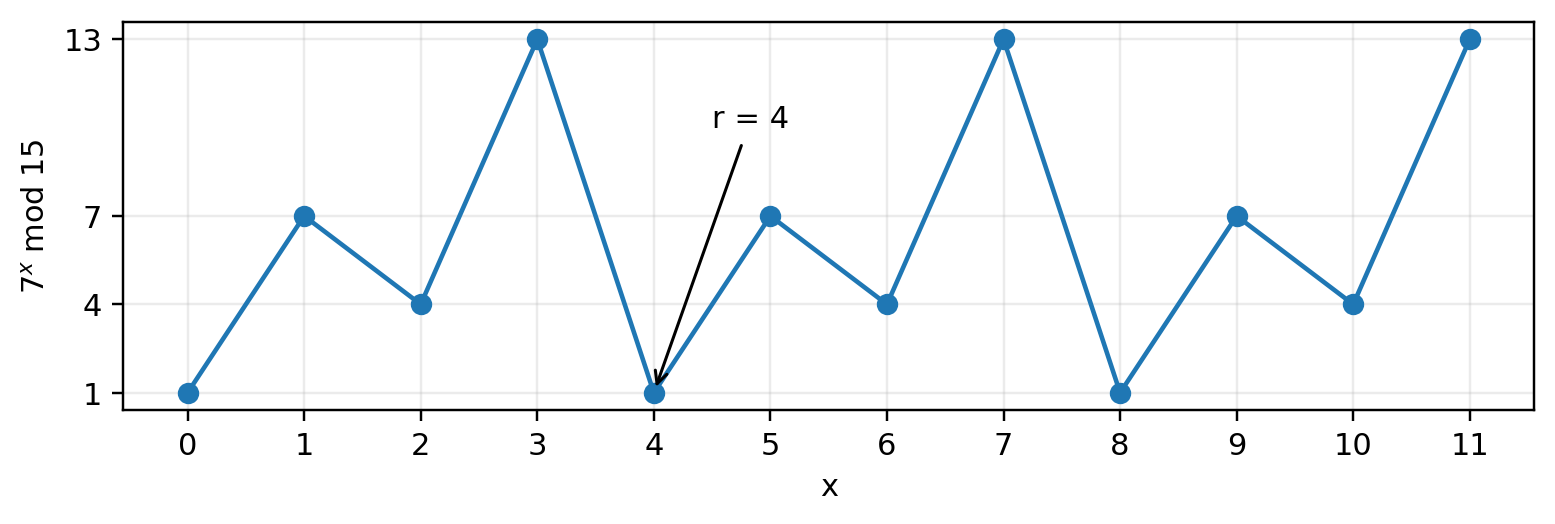
\includegraphics[width=0.85\textwidth,height=0.60\textheight,keepaspectratio]{finale_fig_3_1_periodicita_n15.png}

\caption{Periodicità di $7^x\bmod 15$: la sequenza si ripete ogni quattro valori, quindi $r=4$.}\label{fig:finale_3_1}
\end{figure}

\subsection{Quantum Phase Estimation e Quantum Fourier Transform}\label{sec:finale_3_2_2}

Il nucleo quantistico stima la fase dell'operatore di moltiplicazione modulare tramite QPE. Un registro di controllo prepara una sovrapposizione, applica potenze controllate dell'operatore e usa la QFT inversa per trasformare la fase in una distribuzione misurabile. Il post-processing classico ricostruisce una frazione vicina a $s/r$ e verifica i fattori candidati. L'AQFT elimina rotazioni di fase piccole: riduce porte e profondità, ma introduce un errore algoritmico che deve essere misurato sulla distribuzione e sulla probabilità finale di fattorizzazione, non soltanto sul conteggio delle porte \cite{barencoAQFT1996,akoramurthy2026}.

\begin{figure}[H]
\centering
\begin{tikzpicture}[
  node distance=5mm,
  every node/.style={execute at begin node=\setstretch{1}},
  box/.style={draw, rounded corners=3pt, thick, align=center, text width=29mm,
              minimum height=24mm, font=\small},
  classico/.style={box, fill=gray!10, draw=gray!70!black},
  quantistico/.style={box, fill=blue!8, draw=blue!55!black},
  freccia/.style={-{Stealth[length=2.6mm]}, thick},
  nota/.style={font=\footnotesize, align=center, text width=31mm, anchor=north}
]
\node[classico] (pre) {\textbf{Pre-processing}\\ classico\\[3pt] scelta di $a$,\\ $\gcd(a,N)$};
\node[quantistico, right=of pre] (pf) {\textbf{Period finding}\\ quantistico\\[3pt] esp.\ modulare\\ + QPE};
\node[quantistico, right=of pf] (qft) {\textbf{QFT}$^{-1}$\\ e misura\\[3pt] esito $y$};
\node[classico, right=of qft] (post) {\textbf{Post-processing}\\ classico\\[3pt] frazioni continue\\ + $\gcd$};
\draw[freccia] (pre) -- (pf);
\draw[freccia] (pf) -- (qft);
\draw[freccia] (qft) -- (post);
\node[nota] at ([yshift=-2.5mm]pre.south) {$N$ composto,\\ $a$ coprimo con $N$};
\node[nota] at ([yshift=-2.5mm]pf.south) {$U_{a,N}\ket{x}\ket{1}$\\ $=\ket{x}\ket{a^x \bmod N}$};
\node[nota] at ([yshift=-2.5mm]qft.south) {$y/2^m \approx s/r$};
\node[nota] at ([yshift=-2.5mm]post.south) {fattori\\ $\gcd(a^{r/2}\pm1,\,N)$};
\draw[decorate, decoration={brace, amplitude=5pt}, thick, blue!55!black]
  ([yshift=2mm]pf.north west) -- ([yshift=2mm]qft.north east)
  node[midway, above=6pt, font=\footnotesize] {eseguito sul processore quantistico};
\end{tikzpicture}

\caption{Pipeline concettuale di Shor: pre-processing classico, period finding quantistico, QFT inversa e post-processing classico. In azzurro le fasi eseguite sul processore quantistico; sotto ciascuna fase la grandezza che la caratterizza.}\label{fig:finale_3_2}
\end{figure}

\subsection{Misura, shot e criterio di successo adottato}\label{sec:finale_3_2_3}

Una singola esecuzione restituisce una bitstring; più shot stimano l'istogramma degli esiti. La tesi distingue la massa utile per singola misura, il successo TOP-$K$ ottenuto verificando i primi $K$ candidati e il numero di iterazioni indipendenti necessario a ricavare i fattori. Il successo viene registrato soltanto quando il post-processing produce fattori non banali verificati moltiplicativamente. Questa definizione rende confrontabili TOP-1, TOP-4, classificatore e AQFT, ma richiede una baseline combinatoria: per $N=15$ la procedura classica accetta 63 esiti su 256 e può quindi produrre un successo residuo anche da una distribuzione quasi uniforme.

\subsection{Costo circuitale e ruolo delle istanze}\label{sec:finale_3_2_4}

Il costo dipende da qubit, porte a due qubit, profondità, routing e aritmetica modulare. $N=15$ consente campagne replicate e confronti controllati; $N=21$ verifica un ordine $r=6$ meno favorevole al troncamento; istanze ulteriori sono usate soltanto per controlli ideali. La tesi non estrapola da queste taglie la fattorizzazione crittografica: le implementazioni fault-tolerant richiedono aritmetica, correzione, feed-forward e operazioni non-Clifford esplicite \cite{beauregard2002,gidney2021,chevignard2025}.

\section{Rumore quantistico e modelli utilizzati}\label{sec:finale_3_3}

\subsection{Sorgenti fisiche rilevanti}\label{sec:finale_3_3_1}\label{sec:fonti_fisiche}

Le campagne distinguono preparazione, rilassamento $T_1$, perdita di coerenza $T_2$, errori di gate, crosstalk e readout. Nei dispositivi reali questi fenomeni possono dipendere da qubit, tempo e routing; il modello uniforme di Shor li separa invece deliberatamente per identificare il contributo delle singole componenti. Gli aspetti fisici e l'anatomia di una QPU sono approfonditi nella Sezione~\ref{app:anatomia}; il mapping operativo adottato nel corpo è illustrato nella Figura~\ref{fig:finale_3_3} \cite{preskill2018,murali2019,tannu2019}.

\begin{figure}[H]
\centering
% Schema vettoriale: riquadri identici e frecce ancorate ai bordi.
\begin{tikzpicture}[
  every node/.style={execute at begin node=\setstretch{1}},
  blocco/.style={draw=blue!55!black, fill=blue!8, rounded corners=3pt, thick,
    minimum width=3.15cm, minimum height=1.25cm, text width=2.85cm,
    align=center, inner sep=3pt, font=\footnotesize},
  freccia/.style={-{Stealth[length=2.2mm]}, thick}
]
\node[blocco] (prep) at (0,0) {\textbf{Preparazione}};
\node[blocco] (mod) at (3.9,0) {\textbf{Esponenziazione}\\modulare};
\node[blocco] (qft) at (7.8,0) {QFT$^{-1}$};
\node[blocco] (mis) at (11.7,0) {\textbf{Misura}};
\node[blocco, fill=gray!10, draw=gray!70!black] (errprep) at (0,-2.25) {Errori di\\preparazione};
\node[blocco, fill=gray!10, draw=gray!70!black] (errmod) at (3.9,-2.25) {Decoerenza +\\errori 2Q};
\node[blocco, fill=gray!10, draw=gray!70!black] (errqft) at (7.8,-2.25) {Errori di fase +\\rumore di gate};
\node[blocco, fill=gray!10, draw=gray!70!black] (errmis) at (11.7,-2.25) {Readout};
\draw[freccia] (prep.east) -- (mod.west);
\draw[freccia] (mod.east) -- (qft.west);
\draw[freccia] (qft.east) -- (mis.west);
\draw[freccia] (errprep.north) -- (prep.south);
\draw[freccia] (errmod.north) -- (mod.south);
\draw[freccia] (errqft.north) -- (qft.south);
\draw[freccia] (errmis.north) -- (mis.south);
\node[font=\small, align=center] at (5.85,1.3)
  {Crosstalk e vincoli topologici agiscono trasversalmente};
\end{tikzpicture}

\caption{Collocazione concettuale delle principali sorgenti di rumore nella pipeline di Shor.}\label{fig:finale_3_3}
\end{figure}

\subsection{Canali elementari e convenzione depolarizzante}\label{sec:finale_3_3_2}

Il rilassamento e il dephasing sono parametrizzati attraverso $T_1$, $T_2$ e la durata delle operazioni; il readout è descritto da una matrice di confusione. Per i gate, Qiskit Aer usa un canale depolarizzante parametrizzato da $\lambda$, che non coincide in generale con la probabilità aggregata di applicare un Pauli non identità. La convenzione esatta e le derivazioni complete sono riportate nella Sezione~\ref{app:canali} e devono essere mantenute quando si confrontano campagne differenti \cite{qiskit2023,nielsenChuang2000}.

\subsection{Modello di rumore della campagna Shor N=15}\label{sec:finale_3_3_3}

La campagna principale usa preset uniformi e controllati per porte a uno e due qubit, rilassamento e readout. Non rappresenta la calibrazione di una QPU specifica: serve a confrontare strategie sugli stessi istogrammi, con seed e netlist condivisi. I preset, gli sweep e le numerosità sono dichiarati nella Sezione~\ref{sec:finale_3_5} e nelle Sezioni~\ref{app:parametrica} e~\ref{app:obiettivi}; i controlli hardware-aware usano invece una snapshot offline separata.

\subsection{Tre grandezze d'errore che non vanno confuse}\label{sec:finale_3_3_4}

La Tabella~\ref{tab:finale_3_3} impedisce di sovrapporre tre livelli sperimentali distinti. Non viene costruita una conversione numerica fra $p_L$ e $p_g$: richiederebbe una compilazione fault-tolerant completa dell'algoritmo.

\begin{table}[!htbp]
\centering
\small

\begin{tabularx}{\textwidth}{@{}lXX@{}}
\toprule
\textbf{Simbolo} & \textbf{Significato} & \textbf{Uso} \\
\midrule
$p$ & Intensità dell'errore fisico del modello. & Memory experiment QEC e stima della soglia. \\
\addlinespace[0.3em]
$p_L$ & Probabilità di fallimento logico dopo decodifica. & Confronto fra distanze e decoder. \\
\addlinespace[0.3em]
$p_g$ & Proxy Pauli totale applicato dopo ciascun gate compilato. & Sensibilità locale del circuito di Shor. \\
\bottomrule
\end{tabularx}
\caption{Convenzione delle grandezze d'errore usata nella versione revisionata.}\label{tab:finale_3_3}

\end{table}

\section{Strategie di intervento considerate}\label{sec:finale_3_4}

\subsection{Post-processing e mitigazione a valle della misura}\label{sec:finale_3_4_1}

TOP-$K$ modifica soltanto la ricerca classica sui candidati già presenti nell'istogramma; il classificatore decide quando applicarla; la ZNE varia artificialmente il rumore per estrapolare un osservabile. Queste strategie non correggono lo stato quantistico e devono essere valutate sul costo finale della fattorizzazione. Per questo DR1 include l'ablazione TOP-4 senza classificatore e una baseline combinatoria, mentre i dettagli degli sweep e della ZNE sono conservati nella Sezione~\ref{app:parametrica} \cite{temme2017,liBenjamin2017}.

\subsection{Quantum Error Correction: sindrome, distanza e soglia}\label{sec:finale_3_4_2}

La QEC codifica l'informazione logica in più qubit e misura stabilizzatori che rivelano la sindrome senza leggere direttamente lo stato logico. La distanza $d$ determina il numero di errori correggibili; nel surface code l'aumento di $d$ è utile soltanto sotto una soglia dipendente da circuito, rumore e decoder. La tesi procede per livelli: repetition code come verifica analitica, Steane $[[7,1,3]]$ come codice stabilizer e surface code ruotato come famiglia scalabile \cite{shorcorrection1995,steane1996,fowler2012,dennis2002topological,googleQECBelowThreshold2025}.

Il surface code paga la località con un costo elevato: ogni patch protegge un solo qubit logico e richiede $d^2$ qubit di dato. I codici quantum Low-Density Parity-Check (qLDPC) rinunciano alla località stretta per codificare più qubit logici nello stesso blocco, mantenendo controlli di peso limitato. Il Gross code proposto da IBM, un codice bivariate bicycle $[[144,12,12]]$, codifica 12 qubit logici in 144 qubit di dato con distanza 12 e controlli di peso 6 \cite{bravyi2024}. Nella tesi è studiato nel modello code-capacity, cioè con errori sui soli qubit di dato e sindromi perfette: un modello più semplice di quello circuit-level del surface code, adatto a confrontare codici diversi a parità di rumore, ma non a stimare il costo dell'estrazione delle sindromi. Per questi codici il matching non è applicabile in modo diretto e il decoder di riferimento è BP+OSD \cite{roffe2020,panteleev2021}.

\begin{figure}[H]
\centering
\begin{tikzpicture}[
  every node/.style={execute at begin node=\setstretch{1}},
  blocco/.style={draw=blue!55!black, fill=blue!8, rounded corners=3pt, thick,
    minimum width=2.55cm, minimum height=1.45cm, text width=2.3cm,
    align=center, inner sep=3pt, font=\small},
  freccia/.style={-{Stealth[length=2.2mm]}, thick}
]
\node[blocco] (cod) at (0,0) {Codifica\\stato logico};
\node[blocco] (rum) at (3.05,0) {Rumore\\fisico};
\node[blocco] (stab) at (6.1,0) {Misura degli\\stabilizzatori};
\node[blocco, fill=gray!10, draw=gray!70!black] (dec) at (9.15,0) {Decoder\\[2pt]\footnotesize sindrome\\$\to$ decisione};
\node[blocco, fill=gray!10, draw=gray!70!black] (esito) at (12.2,0) {Esito\\logico};
\draw[freccia] (cod.east) -- (rum.west);
\draw[freccia] (rum.east) -- (stab.west);
\draw[freccia] (stab.east) -- (dec.west);
\draw[freccia] (dec.east) -- (esito.west);
\node[font=\small, align=center, text width=14.7cm] at (6.1,1.4)
  {La sindrome rivela l'errore senza misurare direttamente l'informazione logica};
\node[font=\small, align=center, text width=14.7cm] at (6.1,-1.5)
  {MWPM / BP+OSD / rete / decoder ibrido\\
   operano sul medesimo flusso di detection events};
\end{tikzpicture}

\caption{Ciclo concettuale della QEC e posizione dei decoder analitici o appresi.}\label{fig:finale_3_4}
\end{figure}

\subsection{Decoder analitici, appresi e ibridi}\label{sec:finale_3_4_3}

MWPM interpreta i detection events tramite un grafo; BP+OSD combina belief propagation e una ricerca ordinata; il decoder appreso può sostituire la baseline oppure correggerne residualmente gli errori. Il confronto corretto usa gli stessi campioni e lo stesso modello nominale: una rete è scientificamente utile soltanto se recupera struttura non rappresentata dalla migliore baseline analitica plausibile. Disegno completo, controlli E1--E12 e matrici di trasferimento sono nella Sezione~\ref{app:decodifica} \cite{pymatching2021,roffe2020,panteleev2021,alphaqubit2024,torlaiMelko2017}.

In BP+OSD la belief propagation scambia messaggi fra qubit e controlli per stimare la probabilità d'errore di ciascun qubit; se non converge a una correzione coerente con la sindrome, l'ordered statistics decoding usa quelle stime per risolvere il sistema lineare sui qubit più sospetti. L'ordine in cui i messaggi vengono aggiornati, tutti insieme (parallelo) o uno alla volta (seriale), non cambia il codice ma può cambiare molto la qualità della decodifica: la Sezione~\ref{sec:finale_5_3_8} mostra che sul Gross code questa sola scelta sposta il fallimento logico di circa due ordini di grandezza.

\subsection{AQFT come ottimizzazione algoritmica}\label{sec:finale_3_4_4}

L'AQFT riduce rotazioni controllate e costo di routing accettando una perdita controllata di precisione. Il grado non viene scelto sul test: ogni campagna separa selection e holdout e misura congiuntamente successo, porte entangling e profondità. La domanda non è quindi se l'AQFT sia sempre migliore, ma quando il rumore evitato superi l'informazione di fase persa \cite{barencoAQFT1996,akoramurthy2026}.
\section{Disegno sperimentale e criteri di inferenza}\label{sec:finale_3_5}

Il disegno complessivo segue un principio comune: baseline esplicita, appaiamento dei campioni quando possibile, separazione tra selezione e test e uso di metriche coerenti con il compito. La Figura~\ref{fig:finale_3_5} riassume le cinque linee corrispondenti alle domande DR1--DR5 del Capitolo 2. I dettagli implementativi --- organizzazione del codice, versioni software e struttura degli artefatti --- sono descritti nel Capitolo 4; qui restano le scelte che determinano la validità dell'inferenza.

\begin{figure}[H]
\centering
\begin{tikzpicture}[
  every node/.style={execute at begin node=\setstretch{1}},
  dr/.style={draw=blue!55!black, fill=blue!8, thick, rounded corners=3pt, align=center,
             text width=24mm, minimum height=25mm, font=\footnotesize},
  met/.style={draw=gray!70!black, fill=gray!10, thick, rounded corners=3pt, align=center,
              text width=24mm, minimum height=22mm, font=\footnotesize},
  freccia/.style={-{Stealth[length=2.2mm]}, thick}
]
\node[draw, thick, rounded corners=3pt, fill=white, align=center, text width=128mm,
      font=\small, inner sep=5pt] (top) at (0,0)
  {\textbf{Contratto sperimentale comune}\\[2pt]
   {\footnotesize baseline esplicita \,$\cdot$\, stessi campioni quando possibile\\
   selezione separata dal test \,$\cdot$\, metriche non intercambiabili}};
\foreach \i/\x/\dom/\met in {
  1/-60/{\textbf{DR1}\\ Post-processing\\ TOP-$K$ / ML}/{iterazioni\\ Wilcoxon + Holm},
  2/-30/{\textbf{DR2}\\ QEC\\ codici e soglia}/{$p_L$, soglia\\ fit di scala},
  3/0/{\textbf{DR3}\\ Decoder\\ analitico / ML}/{$\Delta p_L$ appaiato\\ McNemar},
  4/30/{\textbf{DR4}\\ Shor\\ proxy $p_g$}/{$P_{\mathrm{succ}}$\\ Wilson 95\%},
  5/60/{\textbf{DR5}\\ AQFT\\ troncamento\\ QFT}/{successo + porte\\ selezione\\ holdout}} {
  \node[dr] (d\i) at (\x mm,-35mm) {\dom};
  \node[met] (m\i) at (\x mm,-68mm) {\met};
  \draw[freccia] (d\i) -- (m\i);
}
% linea di distribuzione dal contratto alle cinque domande
\draw[thick] (top.south) -- ++(0,-5mm) coordinate (bus);
\draw[thick] (d1.north |- bus) -- (d5.north |- bus);
\foreach \i in {1,...,5} \draw[freccia] (d\i.north |- bus) -- (d\i.north);
\end{tikzpicture}

\caption{Disegno sperimentale unificato. Le cinque campagne condividono il criterio di confronto, ma non la stessa unità di misura.}\label{fig:finale_3_5}
\end{figure}

La riproducibilità viene trattata come parte del metodo e non come proprietà accessoria del codice. Ogni campagna registra i parametri di input, il seed, la numerosità, le versioni software e gli identificativi della compilazione. Quando più strategie devono essere confrontate, esse ricevono gli stessi campioni oppure una sequenza di seed condivisa. Questa scelta riduce la varianza del confronto e impedisce che una realizzazione casuale favorevole venga scambiata per un vantaggio del metodo.

La separazione selection/validation/holdout è applicata quando il metodo contiene una scelta adattiva. Il classificatore viene selezionato sulla validation e valutato sul test indipendente; la soglia del decoder ibrido viene scelta prima del test; il grado AQFT viene selezionato su batch dedicati e misurato su holdout disgiunti. Il principio è identico nei tre casi: il dato usato per scegliere una configurazione non può essere riutilizzato come prova della sua prestazione.

L'appaiamento viene preferito quando due metodi possono essere applicati allo stesso campione. In DR1 le strategie leggono lo stesso istogramma; in DR3 i decoder ricevono gli stessi detection events; nei confronti AQFT i bracci condividono layout e sequenza dei seed. L'appaiamento elimina dal confronto una parte della variabilità Monte Carlo e rende il test sensibile alla differenza fra metodi, non alla differenza fra campioni casuali. Quando il confronto non può essere appaiato in senso stretto, l'incertezza viene riportata esplicitamente tramite intervalli binomiali o bootstrap.

Le correzioni per confronti multipli vengono applicate alla famiglia inferenziale dichiarata, non indiscriminatamente a tutte le analisi esplorative della tesi. Questo permette di distinguere gli endpoint principali, per i quali il controllo dell'errore di I tipo è parte del contratto, dagli sweep esplorativi usati per generare ipotesi. Nel Capitolo 5 le due categorie vengono indicate separatamente.

\subsection{Perimetro delle istanze e validazione funzionale}\label{sec:finale_3_5_1}

\begingroup
\small
\begin{table}[!htbp]
\centering
\small

\begin{tabular}{@{}
  >{\raggedright\arraybackslash}p{(\linewidth - 4\tabcolsep) * \real{0.3485}}
  >{\raggedright\arraybackslash}p{(\linewidth - 4\tabcolsep) * \real{0.3163}}
  >{\raggedright\arraybackslash}p{(\linewidth - 4\tabcolsep) * \real{0.3352}}@{}}
\toprule
\textbf{Oggetto} & \textbf{Ruolo} & \textbf{Validazione/\allowbreak{}uso} \\
\midrule
N=15, a=7, r=4 & campagna Shor rumorosa principale & truth table, picchi ideali, fattori 3 e 5; TOP-K/\allowbreak{}ML; M8/M13; AQFT pilota \\
\addlinespace[0.3em]
N=21, a=2, r=6 & aritmetica reversibile e AQFT esplorativa & azione modulare, ancille a zero, QPE ideale; compilazioni e test AQFT a budget ridotto \\
\addlinespace[0.3em]
N=35, a=6, r=2 & controllo ideale aggiuntivo & correttezza dell'aritmetica e distribuzione QPE; nessuna campagna rumorosa principale \\
\addlinespace[0.3em]
memory experiment QEC & caratterizzazione separata della protezione & repetition, Steane, surface code e decoder; nessun trasferimento diretto a Shor \\
\bottomrule
\end{tabular}
\caption{Ruolo delle istanze e separazione dei livelli sperimentali.}\label{tab:finale_3_5}

\end{table}
\endgroup

La validazione dell'aritmetica precede l'uso del successo finale come metrica. Per N=21 e N=35 vengono controllati l'operatore modulare sui vettori validi, l'uncomputation delle ancille e la distribuzione QPE ideale. Questo controllo è necessario perché un post-processing permissivo può restituire occasionalmente fattori anche da un circuito non corretto.

Per N=15 viene applicato lo stesso principio al moltiplicatore ×7 mod 15: la truth table e il periodo atteso vengono verificati prima delle campagne rumorose. Il manifest della netlist compilata conserva conteggi, profondità, base di gate, livello di ottimizzazione e hash della sequenza. In questo modo training del classificatore, baseline e sweep non possono riferirsi accidentalmente a revisioni differenti del circuito.

\begingroup
\small
\begin{table}[!htbp]
\centering
\small

\begin{tabular}{@{}
  >{\raggedright\arraybackslash}p{(\linewidth - 4\tabcolsep) * \real{0.3232}}
  >{\raggedright\arraybackslash}p{(\linewidth - 4\tabcolsep) * \real{0.3923}}
  >{\raggedright\arraybackslash}p{(\linewidth - 4\tabcolsep) * \real{0.2845}}@{}}
\toprule
\textbf{Campagna} & \textbf{Campionamento principale} & \textbf{Unità di analisi} \\
\midrule
DR1 confronto M1/TOP-4/M2 & 30 repliche; 1024 shot per iterazione; max 50 iterazioni & replica appaiata \\
\addlinespace[0.3em]
Classifier DR1 & 2000 istogrammi per scenario; split 60/20/20 & istogramma \\
\addlinespace[0.3em]
Repetition & 20.000 campioni per punto & shot logico \\
\addlinespace[0.3em]
Steane & 200.000 campioni per punto & shot logico \\
\addlinespace[0.3em]
Surface code & 2×10⁵ -- 4×10⁷ shot per punto & shot logico / detection events \\
\addlinespace[0.3em]
Decoder appreso & 4×10⁵ o 8×10⁵ campioni per punto & shot appaiato \\
\addlinespace[0.3em]
M8 sensibilità Shor & 20×4096 shot per punto & shot; replica per dispersione \\
\addlinespace[0.3em]
AQFT N=15 & 8192 shot per grado, split 4/4 batch & batch selection/\allowbreak{}holdout \\
\addlinespace[0.3em]
QPE AQFT & 4096 shot per grado, 3 fasi × 3 taglie & batch selection/\allowbreak{}holdout \\
\bottomrule
\end{tabular}
\caption{Numerosità principali. Le unità statistiche differiscono tra campagne e non vengono aggregate tra loro.}\label{tab:finale_3_6}

\end{table}
\endgroup

Gli artefatti sperimentali sono versionati e accompagnati da manifest. Per i circuiti di Shor il manifest registra almeno N, a, numero di qubit di conteggio, base di gate, optimization level, seed del transpiler, profondità, conteggio delle operazioni e hash della netlist. Per le campagne statistiche vengono salvati anche seed del simulatore, vettori appaiati, parametri del noise model, definizione delle etichette e versione dello schema dati. Questo consente di distinguere un cambio del metodo da un cambio del circuito o dell'ambiente.

Gli output di implementazioni successivamente riconosciute come errate non vengono mantenuti come evidenza corrente. In particolare, le campagne sono state rigenerate dopo la correzione del moltiplicatore ×7 mod 15 e, nell'AQFT, gli output della prima variante senza SWAP sono esclusi dopo la correzione della permutazione. Questa politica evita un problema frequente nei lavori sperimentali iterativi: utilizzare risultati numericamente plausibili prodotti da una revisione del codice che non implementa più il contratto dichiarato.

\subsection{DR1 - Post-processing, classificatore e ablazione}\label{sec:finale_3_5_2}

Il confronto principale usa il circuito N=15, a=7 compilato una sola volta nella base rz/sx/x/cx, optimization level 2 e seed di transpiler fissato. La netlist di riferimento contiene 224 CX e ha profondità 412. Ogni iterazione genera un singolo istogramma da 1024 shot, consegnato senza ricampionamento a TOP-1, TOP-4 e M2. Le differenze tra strategie dipendono quindi dalla regola decisionale e non da realizzazioni Monte Carlo diverse.

\begin{figure}[H]
\centering
\begin{tikzpicture}[
  every node/.style={execute at begin node=\setstretch{1}},
  blocco/.style={draw=blue!55!black, fill=blue!8, rounded corners=3pt, thick,
    minimum width=3.6cm, minimum height=1.35cm, text width=3.25cm,
    align=center, inner sep=3pt, font=\small},
  freccia/.style={-{Stealth[length=2.2mm]}, thick},
  linea/.style={thick}
]
\node[blocco, minimum height=1.8cm, fill=gray!10, draw=gray!70!black] (sim) at (0,0)
  {Una simulazione\\$N=15$ $\to$ istogramma};
\node[blocco] (top1) at (5.5,2) {\textbf{TOP-1}};
\node[blocco] (top4) at (5.5,0) {\textbf{TOP-4}};
\node[blocco] (m2) at (5.5,-2) {\textbf{M2}: ML + TOP-4};
\node[blocco, minimum height=1.8cm, fill=gray!10, draw=gray!70!black] (test) at (11,0)
  {Vettori appaiati\\primo successo\\Wilcoxon / Holm};
% Due linee verticali comuni evitano diagonali e incroci.
\coordinate (ingresso) at (2.75,0);
\coordinate (uscita) at (8.25,0);
\draw[linea] (sim.east) -- (ingresso);
\draw[linea] (2.75,2) -- (2.75,-2);
\draw[freccia] (2.75,2) -- (top1.west);
\draw[freccia] (ingresso) -- (top4.west);
\draw[freccia] (2.75,-2) -- (m2.west);
\draw[linea] (top1.east) -- (8.25,2);
\draw[linea] (top4.east) -- (uscita);
\draw[linea] (m2.east) -- (8.25,-2);
\draw[linea] (8.25,2) -- (8.25,-2);
\draw[freccia] (uscita) -- (test.west);
\fill (ingresso) circle (1.3pt);
\fill (uscita) circle (1.3pt);
\node[font=\small, align=center, text width=14.4cm] at (5.5,3.15)
  {Le tre strategie ricevono gli stessi conteggi e la stessa regola di tie-break};
\end{tikzpicture}

\caption{Pipeline appaiata della campagna DR1: una sola simulazione alimenta TOP-1, TOP-4 e M2.}\label{fig:finale_3_6}
\end{figure}

Oltre ai due preset principali, la robustezza della regola TOP-K viene esplorata variando un fattore alla volta. Lo scopo degli sweep non è stimare una legge causale generale, ma verificare se il comportamento osservato sia fragile rispetto a scelte ragionevoli del contratto. Le famiglie considerate sono riassunte nella Tabella~\ref{tab:finale_3_7}. Poiché gli sweep appartengono a famiglie esplorative differenti, i loro p-value non vengono corretti globalmente come se costituissero un unico test definito a priori.

\begingroup
\small
\begin{table}[!htbp]
\centering
\small

\begin{tabular}{@{}
  >{\raggedright\arraybackslash}p{(\linewidth - 4\tabcolsep) * \real{0.3203}}
  >{\raggedright\arraybackslash}p{(\linewidth - 4\tabcolsep) * \real{0.3352}}
  >{\raggedright\arraybackslash}p{(\linewidth - 4\tabcolsep) * \real{0.3445}}@{}}
\toprule
\textbf{Famiglia di sweep} & \textbf{Variabile controllata} & \textbf{Domanda metodologica} \\
\midrule
Numero di candidati & K = 1,2,3,4,6,8 & quanto beneficio deriva dall'allargare la ricerca \\
\addlinespace[0.3em]
Errore 2Q & $\lambda_{2q}$ da 10⁻³ a 10⁻¹ & robustezza alla componente dominante sui gate entangling \\
\addlinespace[0.3em]
Shot & 128--2048 & dipendenza dalla risoluzione dell'istogramma \\
\addlinespace[0.3em]
K × $\lambda_{2q}$ & griglia congiunta & interazione tra rumore e ampiezza della ricerca \\
\addlinespace[0.3em]
Coerenza & T1/T2 da 20/16 a 500/400 μs & sensibilità al rilassamento/\allowbreak{}dephasing \\
\addlinespace[0.3em]
Errore 1Q & $\lambda_{1q}$ da 10⁻⁴ a 2×10⁻² & ruolo dei gate a singolo qubit \\
\addlinespace[0.3em]
Readout & 0--20\% & effetto della misura imperfetta \\
\addlinespace[0.3em]
Compilazione & optimization level 0--3 & dipendenza dalla netlist prodotta \\
\bottomrule
\end{tabular}
\caption{Sweep esplorativi della campagna DR1 e domanda associata.}\label{tab:finale_3_7}

\end{table}
\endgroup

\begingroup
\small
\begin{table}[!htbp]
\centering
\small

\begin{tabular}{@{}
  >{\raggedright\arraybackslash}p{(\linewidth - 4\tabcolsep) * \real{0.3601}}
  >{\raggedright\arraybackslash}p{(\linewidth - 4\tabcolsep) * \real{0.3333}}
  >{\raggedright\arraybackslash}p{(\linewidth - 4\tabcolsep) * \real{0.3065}}@{}}
\toprule
\textbf{Parametro} & \textbf{Scenario di riferimento} & \textbf{Scenario di stress} \\
\midrule
N / a / r & 15 / 7 / 4 & 15 / 7 / 4 \\
\addlinespace[0.3em]
qubit di controllo / shot & 8 / 1024 & 8 / 1024 \\
\addlinespace[0.3em]
$\lambda_{1q}$ / $\lambda_{2q}$ & 10⁻³ / 10⁻² & 5×10⁻³ / 5×10⁻² \\
\addlinespace[0.3em]
T1 / T2 & 100 / 80 μs & 50 / 30 μs \\
\addlinespace[0.3em]
readout simmetrico $p_{\mathrm{ro}}$ & 0,02 & 0,05 \\
\bottomrule
\end{tabular}
\caption{Preset uniformi della campagna Shor N=15. Sono scenari controllati, non snapshot di una QPU. I parametri $\lambda_{1q}$ e $\lambda_{2q}$ corrispondono rispettivamente a $\epsilon_{1q}$ e $\epsilon_{2q}$ nella descrizione estesa; $1\,\mu\mathrm{s}=1000\,\mathrm{ns}$.}\label{tab:finale_3_8}

\end{table}
\endgroup

Per ciascuno scenario vengono eseguite 30 repliche appaiate, con un massimo di 50 iterazioni. Un fallimento entro il budget è codificato con il valore 51 in modo da non scomparire dai vettori inferenziali. I pareggi di frequenza sono risolti con una priorità deterministica dipendente dal seed e dalla bitstring, così il ranking non dipende dall'ordine del dizionario o dal valore numerico dell'esito.

Il dataset del classificatore è costruito separatamente: 2000 istogrammi per scenario, ciascuno da 1024 shot. I cinque parametri del rumore uniforme (λ₁q, λ₂q, T1, T2 e readout) sono campionati indipendentemente entro ±50\% del preset. I dati sono separati in train, validation e test nelle proporzioni 60/20/20. Random Forest, SVM RBF calibrata e MLP vengono confrontati sulla validation; il modello selezionato viene rifittato su train+validation e valutato una sola volta sul test indipendente. F1 e AUC descrivono la capacità predittiva, ma la metrica operativa primaria resta il numero di iterazioni necessarie a fattorizzare.

L'etichetta operativa principale del dataset è TOP-1: vale uno quando il candidato dominante conduce a fattori. Una seconda etichetta TOP-16 è mantenuta come audit, non come target finale. Se tutti i campioni risultano positivi per una regola, il runner interrompe l'addestramento invece di forzare un classificatore costante. Questo controllo impedisce di confondere una classe quasi sempre positiva per ragioni combinatorie con un compito predittivo informativo.

Il vettore di ingresso è l'istogramma normalizzato sui 256 esiti. Di conseguenza, il classificatore osserva l'intera distribuzione già campionata: non decide se eseguire o meno il circuito e non risparmia gli shot necessari a costruire l'istogramma. L'eventuale vantaggio deve quindi emergere dalla riduzione delle iterazioni future, non dall'accuratezza di classificazione presa isolatamente.

I confronti M1\textgreater TOP-4 e M1\textgreater M2 usano il test di Wilcoxon appaiato con \verb|zero_method='pratt'| e alternativa unilaterale; TOP-4 versus M2 è bilaterale. I p-value appartenenti alla stessa famiglia vengono corretti con Holm. Questa struttura rende l'ablazione parte integrante dell'ipotesi: un classificatore è utile solo se migliora la stessa ricerca multi-candidato senza filtro.

Il ricorso al Wilcoxon è coerente con la natura discreta e fortemente asimmetrica della metrica: il numero di iterazioni è piccolo, molti confronti producono differenza zero e i fallimenti vengono conservati come sentinella. La variante Pratt mantiene le coppie con differenza zero nel calcolo dei ranghi in modo appropriato al disegno. Medie e rapporti ρ vengono riportati come descrittivi, ma la decisione inferenziale usa l'intero vettore appaiato.

Le metriche del classificatore vengono calcolate sul test indipendente, mentre l'utilità operativa viene misurata nelle 30 repliche del confronto M1/TOP-4/M2. I due livelli non sono equivalenti: F1 e AUC rispondono alla domanda ``il modello predice l'etichetta?'', il numero di iterazioni risponde alla domanda ``il modello riduce il costo della fattorizzazione?''. Questa separazione è centrale per evitare che una buona accuratezza venga presentata come prova di un beneficio che non è stato misurato.

Il confronto ZNE usa due o tre livelli di rumore depolarizzante. Poiché ogni livello richiede nuove esecuzioni, il costo viene riportato anche in shot complessivi; il confronto non usa il solo tasso di successo.

\subsection{DR2 - Protocolli QEC e stima della soglia}\label{sec:finale_3_5_3}

Il codice a ripetizione a tre qubit è verificato sia tramite iniezioni deterministiche, sia con 20.000 campioni per punto. Il riferimento analitico è p\_L=3p²-2p³: la concordanza serve come controllo della pipeline di sindrome e decodifica. Il laboratorio distingue la variante bit-flip dalla variante phase-flip, perché il codice protegge un solo tipo di errore per volta.

Per Steane \ensuremath{[[7,1,3]]} vengono verificati i 21 casi di errore singolo X, Y e Z sui sette qubit e la preparazione del code space. Lo sweep quantitativo usa un modello di Pauli e 200.000 campioni per punto. L'estrazione della sindrome è idealizzata: p\_L misura quindi la capacità del codice e della lookup table nel modello adottato, non una procedura fault-tolerant completa. La pendenza log-log a piccolo p e la regione p\_L\textless p sono le metriche principali.

Il surface code ruotato viene simulato con Stim \cite{stim2021} e decodificato con PyMatching \cite{pymatching2021}. La campagna copre d=3,5,7,9, memorie in base X e Z, rounds=d e p tra 2×10⁻³ e 10⁻². Il campionamento è adattivo, da 2×10⁵ a 4×10⁷ shot per punto, per raccogliere un numero sufficiente di fallimenti logici. La soglia viene valutata sia dall'inversione dell'ordine delle curve sia dal fit dell'Equazione (3.6) nel regime sotto soglia. Gli intervalli riportati sono binomiali e la seconda esecuzione indipendente funge da controllo di riproducibilità. La scelta delle distanze e l'interpretazione sotto-soglia sono coerenti con la letteratura del surface code e con le recenti dimostrazioni sperimentali di scaling logico \cite{fowler2012,googleQECBelowThreshold2025,googleSurfaceCode2023,dennis2002topological}.

Nel circuito surface-code il parametro p viene applicato a più punti del ciclo: depolarizzazione dopo gate Clifford, flip dopo reset e prima della misura. Il detector error model viene ricavato dal circuito e fornito a PyMatching. L'errore logico è stimato confrontando la predizione del decoder con l'osservabile logico restituito dal campionatore. Il numero di round pari a d permette di includere la dimensione temporale della sindrome invece di valutare soltanto un singolo snapshot.

La stima della soglia viene mantenuta separata dalla pseudo-soglia di Steane. Nel codice a distanza fissa, il punto p\_L=p indica un break-even del laboratorio considerato; nel surface code la soglia è una proprietà emergente dal confronto tra più distanze. Usare lo stesso termine per i due oggetti renderebbe ambiguo il significato fisico delle curve.

Nei punti in cui p\_L è molto piccolo, un numero fisso di shot produrrebbe pochi o nessun fallimento osservato e quindi intervalli poco informativi. Il campionamento adattivo del surface code aumenta perciò la numerosità fino a raccogliere circa duecento eventi logici per punto, entro il budget massimo. Questa scelta non cambia la definizione della quantità stimata, ma rende confrontabili punti che differiscono di ordini di grandezza nel logical error rate.

L'estrapolazione del fit verso distanze non simulate viene utilizzata soltanto per discutere l'ordine di grandezza del costo di memoria, non come osservazione sperimentale. Quando il Capitolo 5 riporta qubit richiesti a p\_L target molto piccoli, tali valori derivano dall'inversione del modello di scala e devono essere letti con l'incertezza e le assunzioni del fit, non come configurazioni effettivamente simulate.

\subsection{DR3 - Confronto tra decoder analitici e appresi}\label{sec:finale_3_5_4}

Il dataset del decoder coincide con l'output del campionatore Stim: la matrice dei detection events costituisce l'ingresso e l'esito dell'osservabile logico l'etichetta. MWPM e modello appreso ricevono quindi gli stessi campioni. La rete di riferimento è un MLP con due strati nascosti (128,64), attivazione ReLU, ottimizzatore Adam ed early stopping su validation interna.

L'apprendimento è supervisionato: l'etichetta deriva dall'osservabile logico del campionatore, non dalla decisione di MWPM. Nel confronto di sostituzione la rete predice direttamente il flip logico; nel correttore residuale il bersaglio è invece l'evento ``MWPM ha sbagliato''. Cambiare il bersaglio cambia il problema di apprendimento e consente alla rete ibrida di concentrarsi sui casi residuali invece di ricostruire da zero la decodifica completa.

La scelta della soglia del residuo è formulata in termini di costo simmetrico: ribaltare uno shot che MWPM aveva corretto introduce un errore, mentre ribaltare un errore di MWPM ne elimina uno. Per produrre un guadagno netto, la precisione fra gli shot ribaltati deve quindi superare il 50\%. Questa condizione rende evidente perché una AUC superiore a 0,5 non sia, da sola, sufficiente a migliorare p\_L.

La prima prova valuta la sostituzione di MWPM con la rete in condizioni in cui il detector error model fornito al matching è coerente con il rumore simulato. La seconda introduce un crosstalk Pauli correlato tra qubit dati adiacenti, con intensità p\_ct ∈ \{0,005; 0,01; 0,02; 0,04\}, mantenendo p=3×10⁻³. Il modello nominale usato da MWPM non include tale meccanismo, così il confronto misura una mancanza strutturale del decoder e non una semplice variazione di parametro.

Nel decoder ibrido la rete non predice direttamente la correzione: stima se la decisione di MWPM sia errata. La soglia τ è scelta sui dati di validazione e poi congelata sul test; tra le opzioni ammissibili è inclusa l'astensione, equivalente a non ribaltare mai la decisione del matching. Le differenze tra MWPM e ibrido sono valutate con il test di McNemar appaiato sugli stessi shot. Campagne di controllo confrontano inoltre MWPM con BP+OSD sul medesimo detector error model nominale, per verificare se un decoder analitico più espressivo assorba il margine attribuito alla rete.

Le campagne principali usano 4×10⁵ campioni per punto nei confronti di sostituzione e 8×10⁵ per punto nell'ibrido, con partizioni separate per addestramento, validazione e test. Le analisi sulla dimensione dell'ingresso e sulla trasferibilità sono interpretate come controlli di scala, non come prove di universalità del decoder.

Un controllo addizionale varia il numero di round a distanza fissata per separare due fattori che altrimenti crescono insieme: distanza del codice e numero di detector in ingresso alla rete. Questo esperimento è metodologicamente importante perché impedisce di attribuire automaticamente alla distanza una perdita di efficacia che potrebbe dipendere dalla larghezza del vettore di sindrome. Un secondo controllo confronta la soglia scelta onestamente in validation con una soglia oracolo scelta sul test: l'oracolo non è utilizzabile in pratica, ma stabilisce se il limite osservato appartenga alla calibrazione della soglia o alla capacità stessa del modello.

Un confronto esplorativo separato, M16, estende la domanda dal decoder al codice. Il Gross code \ensuremath{[[144,12,12]]} \cite{bravyi2024} è confrontato con 12 patch indipendenti di surface code ruotato, a parità di qubit logici protetti, nel modello code-capacity: errori X indipendenti con probabilità q sui qubit di dato, sindromi perfette, un solo ciclo di correzione. Per la simmetria CSS il settore Z si comporta allo stesso modo e non viene simulato separatamente. La metrica è la probabilità che almeno uno dei 12 qubit logici fallisca; per il surface code si usa 1-(1-p\_L)¹². Il surface code è decodificato con MWPM e, come controllo, con lo stesso BP+OSD del Gross code: le due regole coincidono entro l'incertezza, quindi il confronto non è sbilanciato dal decoder del riferimento. Il modello code-capacity è diverso da quello circuit-level di DR2 e i due insiemi di numeri non vengono confrontati fra loro.

I criteri di adeguatezza sono fissati prima degli approfondimenti: almeno 100 fallimenti per punto, altrimenti si riporta un limite superiore 3/N; intervalli al 95\% con larghezza relativa entro il 20\%; esiti ``migliore'' o ``peggiore'' solo con intervalli non sovrapposti. La configurazione di BP+OSD è scelta con due sweep di dodici varianti ciascuno sugli stessi shot, con test di McNemar appaiato, e confermata su semi indipendenti. A rumore molto basso, dove la simulazione diretta richiederebbe circa 10¹⁰ shot, p\_L è ricostruita dalla decomposizione per peso p\_L(q) = Σ\_w B(w; n, q) f(w), dove B è la binomiale e f(w) la probabilità di fallimento con esattamente w errori: i pesi fino a 5 sono enumerati in modo esaustivo, quelli successivi campionati. La ricostruzione è accettata solo se concorda entro il 20\% con due controlli diretti indipendenti, uno per ciascun codice.

\subsection{DR4 - Sensibilità di Shor a un proxy per gate}\label{sec:finale_3_5_5}

L'esperimento M8 applica dopo ciascun gate sx/x e cx della netlist compilata un canale di Pauli indipendente con probabilità totale p\_g. Le rz restano virtuali. Per rispettare la parametrizzazione di Aer, lo script usa

\begin{equation*}
  \lambda_1 = \tfrac{4}{3}\,p_g, \qquad \lambda_2 = \tfrac{16}{15}\,p_g \tag{3.7}
\end{equation*}

Il circuito resta N=15, a=7. Ogni punto della griglia aggrega 20 repliche indipendenti da 4096 shot, per un totale di 81.920 misure. Un singolo shot è dichiarato riuscito quando il post-processing restituisce fattori non banali. Gli intervalli sul successo sono Wilson al 95\%. La curva misura quindi la sensibilità della specifica implementazione a un residuo Pauli uniforme per gate; non identifica quale codice QEC produrrebbe un determinato p\_g.

Per k tentativi indipendenti, la probabilità cumulativa di almeno un successo viene calcolata come

\begin{equation*}
  P(k) = 1 - (1 - P_s)^k \tag{3.8}
\end{equation*}

Una campagna separata (M13) applica TOP-4 agli stessi livelli di proxy con regole esplicite per i pareggi, per distinguere la robustezza del post-processing dalla massa utile per singola misura.

La griglia di p\_g comprende 0, 10⁻⁴, 5×10⁻⁴, 10⁻³, 1,7×10⁻³, 2×10⁻³, 5×10⁻³, 10⁻², 2×10⁻², 5×10⁻², 10⁻¹, 2×10⁻¹ e 5×10⁻¹. La scelta copre il regime quasi ideale, la zona di degrado e il limite in cui la distribuzione si avvicina al pavimento imposto dal post-processing. Il controllo di monotonia non richiede che ogni differenza tra punti adiacenti sia significativa: verifica che non emergano aumenti incompatibili con l'andamento atteso una volta considerata l'incertezza.

Due controlli hardware-aware, M11 e M11b, utilizzano la snapshot offline FakeSherbrooke. M11 campiona 60 sottografi connessi di 12 qubit e divide 8192 shot per layout in quattro batch di selezione e quattro di holdout; confronta una regola basata sul punteggio di calibrazione con una selezione empirica, usando correlazione di Spearman e bootstrap. M11b studia invece l'associazione tra readout effettivo dopo il routing e successo, controllando per sottografo, numero di ECR e profondità. Entrambi sono studi osservazionali: non addestrano un selettore ML di layout e non autorizzano un claim causale sull'hardware.

M13 affronta un problema specifico del TOP-4 quando più celle hanno lo stesso conteggio al confine del ranking. La regola seeded produce un valore deterministico, ma l'analisi di sensibilità calcola anche scenari favorevoli e sfavorevoli per i pareggi. L'obiettivo non è scegliere a posteriori il risultato più conveniente, bensì quantificare quanto l'endpoint dipenda da una decisione discreta che diventa materiale quando l'istogramma si avvicina all'uniforme.

\subsection{DR5 - Protocollo AQFT e separazione selection/holdout}\label{sec:finale_3_5_6}

La campagna AQFT utilizza una snapshot offline FakeSherbrooke per derivare infedeltà medie di gate e readout. Le rotazioni rz sono virtuali e T1/T2 non vengono aggiunti separatamente nel noise model, evitando un doppio conteggio rispetto all'infedeltà utilizzata. Layout, seed, batch e hash della calibrazione vengono mantenuti nel contratto sperimentale.

Nel pilota Shor N=15, k\_QPE viene variato da 1 a 7, dove 7 corrisponde alla QFT piena. Ogni configurazione usa 8192 shot in otto batch: quattro batch per la selezione del grado e quattro, disgiunti, per l'holdout. La prestazione dichiarata del grado scelto è quindi misurata soltanto sull'holdout. Il confronto registra contemporaneamente successo, porte ECR e profondità compilata.

Per N=21 il troncamento viene applicato alle QFT interne agli addizionatori modulari di Beauregard, lasciando piena la trasformata finale nel confronto primario. Le prove rumorose sono esplorative e hanno budget ridotto: 256 shot per braccio, con 128 shot holdout. I conteggi di porte utilizzati per interpretare il risultato devono provenire dalla stessa compilazione del confronto; conteggi ottenuti da compilazioni differenti non vengono mescolati.

Il benchmark QPE isola infine la sola stima di fase, molto più corta del circuito completo. Sono usati registri da 6, 8 e 10 qubit e tre fasi per dimensione. Ogni grado usa 4096 shot in otto batch, con split 4/4 tra selezione e holdout. Il successo è definito come misura del valore intero più vicino alla fase target alla risoluzione disponibile. Le differenze di proporzione sono accompagnate da intervalli Newcombe al 95\%; i nove confronti sono trattati come esplorativi e non ricevono una correzione simultanea.

\begingroup
\small
\begin{table}[!htbp]
\centering
\small

\begin{tabular}{@{}
  >{\raggedright\arraybackslash}p{(\linewidth - 6\tabcolsep) * \real{0.2041}}
  >{\raggedright\arraybackslash}p{(\linewidth - 6\tabcolsep) * \real{0.2417}}
  >{\raggedright\arraybackslash}p{(\linewidth - 6\tabcolsep) * \real{0.2768}}
  >{\raggedright\arraybackslash}p{(\linewidth - 6\tabcolsep) * \real{0.2774}}@{}}
\toprule
\textbf{Braccio AQFT} & \textbf{Parametro variato} & \textbf{Campionamento} & \textbf{Endpoint} \\
\midrule
Shor N=15 & $k_{\mathrm{QPE}}$ = 1\ldots7 & 8192 shot per grado; 4 batch selection + 4 holdout & successo holdout, ECR, profondità \\
\addlinespace[0.3em]
Shor N=21 & $k_{\mathrm{arith}}$ nelle QFT degli addizionatori & 256 shot per braccio; 128 holdout & differenza troncata-piena, stesso layout \\
\addlinespace[0.3em]
QPE isolata & grado su n=6,8,10; 3 fasi per n & 4096 shot per grado; 4/4 batch & migliore approssimazione della fase, Δ e IC Newcombe \\
\bottomrule
\end{tabular}
\caption{Tre livelli della campagna AQFT. Gli endpoint non vengono aggregati in un'unica metrica.}\label{tab:finale_3_9}

\end{table}
\endgroup

Nel pilota N=15 viene inoltre verificata la rimozione degli SWAP finali. Una prima implementazione che invertiva soltanto l'associazione dei bit alla misura era errata; nella variante corretta la permutazione viene propagata coerentemente nella cascata QFT. Gli output della versione errata sono esclusi dagli artefatti correnti. Questo controllo è mantenuto nel metodo perché mostra un principio generale: un apparente risparmio di porte non è un risultato se cambia l'operatore implementato.

Per N=21 la campagna distingue compilazione strutturale e simulazioni rumorose. I conteggi ECR riportati a supporto di un confronto provengono dalla medesima ricompilazione del braccio pieno e di quello troncato. La stima ausiliaria a miscela, che combina successo ideale e pavimento uniforme, è trattata esclusivamente come modello interpretativo: non sostituisce una simulazione rumorosa né costituisce un limite universale.

\subsection{Minacce alla validità e limiti del disegno}\label{sec:finale_3_5_7}

La validità interna è protetta soprattutto dall'appaiamento, dalla separazione dei dati e dalla validazione funzionale dei circuiti. Restano tuttavia minacce specifiche. Nella campagna Shor N=15 il noise model è uniforme e stazionario e non contiene topologia, crosstalk o deriva; nel surface code il modello principale è stabilizer/Pauli; nelle snapshot FakeSherbrooke la calibrazione è offline e non evolve durante l'esperimento. I risultati devono quindi essere letti come proprietà dei modelli simulati e non come misure di una macchina reale.

La validità esterna è limitata dalle dimensioni delle istanze e dalla scelta dell'ordine r. N=15 ha r=4 e fasi esatte in due bit, una struttura particolarmente favorevole ad alcune forme di troncamento; N=21 ha r=6 e un'aritmetica molto più profonda. Il numero N, da solo, non misura la difficoltà della QPE. Per questo le conclusioni AQFT vengono formulate per istanza e per protocollo, non come proprietà generale della trasformata approssimata.

Anche le conclusioni sul machine learning sono condizionate all'architettura e alle feature usate. Un SVM sull'istogramma finale e un MLP denso sulla sindrome affrontano compiti diversi e dispongono di informazioni diverse; il loro confronto non dimostra che un punto della pipeline sia intrinsecamente ``migliore'' per l'apprendimento. Analogamente, il fatto che BP+OSD possa superare MWPM in alcuni regimi impone di interpretare il guadagno della rete rispetto alla qualità della baseline analitica. Il confronto con il Gross code, infine, vale nel solo modello code-capacity: non include errori di misura, circuito di estrazione delle sindromi né connettività richiesta dall'hardware, e non è confrontabile con le soglie circuit-level del surface code.

Infine, la simulazione end-to-end di Shor fault-tolerant non viene eseguita. Le metriche dei memory experiment, il proxy p\_g e la probabilità di fattorizzazione restano collegate soltanto concettualmente. Qualunque stima di risorse crittografiche richiederebbe un gate set logico, protocolli per le operazioni non-Clifford, scheduling dei cicli di correzione e un modello delle correlazioni residue. Questa assenza è un limite dichiarato del lavoro, non un passaggio colmato mediante estrapolazione.

La validità di costrutto richiede infine che le metriche corrispondano alle domande. TOP-4 misura la probabilità di trovare almeno un candidato verificabile tra i più frequenti, non la qualità dello stato; F1 misura una classificazione, non il costo di fattorizzazione; p\_L misura il fallimento di una memoria codificata, non una porta logica; il conteggio ECR misura il costo compilato, non la fedeltà. La revisione del capitolo rende esplicite queste equivalenze mancate perché molte conclusioni eccessive nascono proprio dal trasferimento implicito tra metriche diverse.

\subsection{Sintesi del contratto sperimentale}\label{sec:finale_3_5_8}

\begingroup
\small
\begin{table}[!htbp]
\centering
\small

\begin{tabular}{@{}
  >{\raggedright\arraybackslash}p{(\linewidth - 8\tabcolsep) * \real{0.1}}
  >{\raggedright\arraybackslash}p{(\linewidth - 8\tabcolsep) * \real{0.21}}
  >{\raggedright\arraybackslash}p{(\linewidth - 8\tabcolsep) * \real{0.23}}
  >{\raggedright\arraybackslash}p{(\linewidth - 8\tabcolsep) * \real{0.23}}
  >{\raggedright\arraybackslash}p{(\linewidth - 8\tabcolsep) * \real{0.23}}@{}}
\toprule
\textbf{DR} & \textbf{Oggetto} & \textbf{Baseline/\allowbreak{}controllo} & \textbf{Metrica primaria} & \textbf{Inferenza} \\
\midrule
DR1 & TOP-K e filtro ML & TOP-1; TOP-4 senza filtro & iterazioni alla fattorizzazione & Wilcoxon appaiato + Holm \\
\addlinespace[0.3em]
DR2 & QEC & qubit fisico / distanze minori & $p_L$, pendenza, $p_{\mathrm{th}}$ & intervalli binomiali + fit \\
\addlinespace[0.3em]
DR3 & decoder & MWPM; BP+OSD & $\Delta p_L$ sugli stessi shot & McNemar; validation separata \\
\addlinespace[0.3em]
DR3 (M16) & Gross code & 12 patch di surface code & P(blocco logico errato) & IC 95\% non sovrapposti; criteri prefissati \\
\addlinespace[0.3em]
DR4 & Shor sotto $p_g$ & $p_g$=0 e baseline uniforme & $P_s$ per shot, P(k) & Wilson 95\%; controlli di monotonia \\
\addlinespace[0.3em]
DR5 & AQFT & QFT piena & successo + ECR/\allowbreak{}profondità & selection/\allowbreak{}holdout; Newcombe \\
\bottomrule
\end{tabular}
\caption{Corrispondenza operativa tra domande di ricerca, baseline, metriche e analisi.}\label{tab:finale_3_10}\label{tab:verifica_requisiti}

\end{table}
\endgroup

Questo contratto è il vincolo interpretativo del Capitolo 5. I risultati delle cinque linee possono essere discussi insieme perché condividono il principio di confronto, ma le loro grandezze non vengono convertite automaticamente l'una nell'altra. In particolare, un miglioramento di TOP-K non equivale a una maggiore fedeltà quantistica, una soglia di memory experiment non determina il successo di Shor e una riduzione di porte AQFT non dimostra da sola un vantaggio sotto rumore.

Un secondo vincolo interpretativo riguarda l'assenza di risultati hardware. Le snapshot di calibrazione vengono usate per costruire modelli riproducibili e confronti controllati, ma non sono misure live della QPU al momento dell'esecuzione. Deriva temporale, leakage, crosstalk reale, routing dipendente dal backend e latenza classica possono alterare il comportamento. La validazione su hardware costituisce pertanto uno sviluppo successivo e non viene anticipata come evidenza sperimentale.

Infine, tutte le conclusioni statistiche restano locali alla famiglia di confronti dichiarata. Dove i test sono esplorativi, questa natura viene esplicitata; dove vengono effettuati confronti multipli definiti a priori, si applica la correzione prevista. L'obiettivo non è massimizzare il numero di differenze significative, ma rendere tracciabile quale evidenza sostiene ciascuna affermazione.

\section{Sintesi metodologica}\label{sec:finale_3_6}

Il capitolo ha definito un quadro unico senza rendere equivalenti esperimenti che misurano oggetti diversi. DR1 valuta l'uso dell'output già misurato, DR2 e DR3 operano sui circuiti di memoria e sulle sindromi, DR4 misura la sensibilità di Shor a un proxy per gate e DR5 modifica il circuito troncando la QFT. I principi comuni sono il confronto con una baseline esplicita, l'uso degli stessi campioni quando possibile e la separazione tra selezione e valutazione. Il Capitolo 4 traduce questo contratto in software, strumenti e artefatti riproducibili.

\chapter{Architettura e implementazione del sistema sperimentale}
\label{chap:implementazione}
\label{chap:sviluppo}
\label{chap:strumenti}


Il Capitolo 3 ha definito il contratto metodologico delle cinque campagne sperimentali. Questo capitolo descrive come tale contratto è stato tradotto in software, circuiti, simulatori e artefatti riproducibili. Non vengono introdotte nuove ipotesi né discussi i risultati: l'obiettivo è rendere verificabile la catena che collega una configurazione dichiarata a un insieme di campioni, a una regola di analisi e infine a un artefatto numerico. La scelta progettuale centrale è la separazione dei livelli: costruzione e compilazione del circuito, esecuzione e rumore, analisi classica, persistenza dei risultati. In questo modo, cambiare un classificatore o un decoder non modifica il campione quantistico su cui viene valutato e una diversa compilazione non può essere confusa con un beneficio dell'algoritmo di analisi.

\section{Ambiente software e strumenti}\label{sec:finale_4_1}

\subsection{Toolchain per le diverse classi di circuito}\label{sec:finale_4_1_1}

La piattaforma usa strumenti differenti in funzione della struttura del circuito. Qiskit e Qiskit Aer \cite{qiskit2023} costruiscono, compilano e simulano l'algoritmo di Shor e gli esperimenti che richiedono circuiti quantistici generali. La campagna rumorosa principale su N=15 usa AerSimulator in modalità statevector; l'analisi di sensibilità M8/M13 impiega matrix\_product\_state per contenere il costo delle molte repliche. I circuiti di Shor contengono rotazioni non-Clifford e non possono quindi essere trasferiti integralmente al formalismo stabilizer.

Per i memory experiment del surface code viene invece utilizzato Stim \cite{stim2021}, che campiona in modo efficiente circuiti stabilizer anche su milioni di shot. Poiché i circuiti di correzione contengono solo porte di Clifford e misure, sono simulabili in modo efficiente su un computer classico: Stim ne campiona le sindromi e i decoder, compresa la rete neurale, sono addestrati e valutati su questi dati. I valori di p\_L riportati sono quindi stime Monte Carlo, non misure su hardware. PyMatching \cite{pymatching2021} costruisce dal detector error model il decoder Minimum Weight Perfect Matching (MWPM). scikit-learn \cite{scikit_learn} viene impiegato sia per il classificatore applicato agli istogrammi di Shor sia per i decoder appresi basati su percettroni multistrato. La libreria ldpc \cite{roffe2020} fornisce BP+OSD, usato come baseline sul surface code e come decoder del Gross code, i cui codici sono costruiti direttamente come matrici di parità con NumPy. Questa separazione della toolchain non è un limite concettuale: riflette classi di circuito diverse e consente di usare, per ciascuna campagna, lo strumento computazionalmente più adatto.

\begingroup
\small
\begin{table}[!htbp]
\centering
\small

\begin{tabular}{@{}
  >{\raggedright\arraybackslash}p{(\linewidth - 4\tabcolsep) * \real{0.3478}}
  >{\raggedright\arraybackslash}p{(\linewidth - 4\tabcolsep) * \real{0.3333}}
  >{\raggedright\arraybackslash}p{(\linewidth - 4\tabcolsep) * \real{0.3188}}@{}}
\toprule
\textbf{Componente} & \textbf{Strumento principale} & \textbf{Ruolo} \\
\midrule
Shor N=15, sweep NISQ & Qiskit + Aer statevector & circuito generale con noise model \\
\addlinespace[0.3em]
Sensibilità M8/M13 & Qiskit + Aer MPS & molte repliche del circuito compilato \\
\addlinespace[0.3em]
Repetition e Steane & Qiskit Aer & laboratori QEC a taglia contenuta \\
\addlinespace[0.3em]
Surface code & Stim + PyMatching & campionamento e MWPM \\
\addlinespace[0.3em]
Classificatori / decoder appresi & scikit-learn & SVM, MLP e correzione residuale \\
\addlinespace[0.3em]
Gross code e codici BB & NumPy + ldpc (BP+OSD) & confronto code-capacity con il surface code \\
\addlinespace[0.3em]
AQFT / topologia & Qiskit Aer & sweep di compilazione e simulazione \\
\bottomrule
\end{tabular}
\caption{Toolchain adottata in funzione della classe di esperimento.}\label{tab:finale_4_1}

\end{table}
\endgroup

\subsection{Ambiente di esecuzione e versionamento}\label{sec:finale_4_1_2}\label{sec:gpu_limit}

Le esecuzioni canoniche sono state orchestrate su CPU in Windows 11 tramite WSL2 con Ubuntu 24.04, Python 3.12 e ambiente virtuale dedicato. La campagna finale registra Qiskit 2.5; Stim 1.16.0 e PyMatching 2.4.0 sono utilizzati per la parte surface-code; la campagna M16 registra ldpc 2.4.1 per BP+OSD. Il file requirements.txt prescrive le dipendenze attese, mentre il manifest di ogni artefatto registra le versioni effettivamente importate di Qiskit, Aer, NumPy, SciPy e scikit-learn. Le due informazioni sono complementari: la prima descrive l'ambiente previsto, la seconda documenta quello realmente impiegato.

Era stata valutata l'accelerazione GPU con una NVIDIA RTX 4070, ma il backend C++ di Aer non risultava disponibile nell'ambiente WSL utilizzato. L'accelerazione GPU non entra quindi nel contratto riproducibile e nessun risultato viene attribuito a prestazioni non misurate. Tutte le campagne riportate sono state eseguite su CPU, condizione registrata nei metadati degli artefatti.

\section{Architettura della piattaforma sperimentale}\label{sec:finale_4_2}

La piattaforma è organizzata in quattro livelli, mantenuti intenzionalmente separati. Il primo costruisce e compila il circuito; il secondo genera i campioni secondo il noise model e i seed dichiarati; il terzo applica la regola di analisi --- post-processing, classificatore o decoder --- senza modificare i campioni; il quarto persiste risultati e metadati e rigenera tabelle e figure. L'architettura impedisce che una modifica a valle alteri implicitamente il circuito o il rumore a monte.

La separazione è applicata anche sul piano dei dati. Gli oggetti prodotti da un livello diventano input immutabili del livello successivo: una netlist compilata viene identificata da conteggi, profondità e hash; un'esecuzione produce conteggi o detection event associati al proprio seed; il post-processing produce metriche senza ricampionare; infine l'artefatto JSON lega risultati e metadati. Questo schema riduce due fonti di bias particolarmente rilevanti nel lavoro: confrontare metodi su campioni differenti e riutilizzare inconsapevolmente un modello addestrato su una revisione diversa del circuito.

\begin{figure}[H]
\centering
\begin{tikzpicture}[
  every node/.style={execute at begin node=\setstretch{1}},
  blocco/.style={draw=blue!55!black, fill=blue!8, thick,
    rounded corners=3pt, align=center, text width=2.7cm,
    minimum height=1.4cm, inner sep=3pt, font=\footnotesize},
  dato/.style={blocco, draw=gray!70!black, fill=gray!10},
  freccia/.style={-{Stealth[length=2.2mm]}, thick}
]

\node[blocco, text width=12.5cm] (costr) at (0,0)
 {\textbf{1. Costruzione e compilazione}\\[3pt]
 Qiskit: circuito, transpile, gate set, layout, hash della netlist};
\node[blocco, text width=12.5cm] (camp) at (0,-2)
 {\textbf{2. Esecuzione e campionamento}\\[3pt]
 Aer / Stim: noise model, shot, seed, detection events};
\node[blocco, text width=12.5cm] (analisi) at (0,-4)
 {\textbf{3. Analisi}\\[3pt]
 TOP-1 / TOP-4 / ML oppure decoder MWPM / rete / ibrido};
\node[dato, text width=12.5cm] (artefatti) at (0,-6)
 {\textbf{4. Artefatti e verifica}\\[3pt]
 JSON schema 2, manifest, metriche, figure e tabelle rigenerate};
\draw[freccia] (costr.south) -- (camp.north);
\draw[freccia] (camp.south) -- (analisi.north);
\draw[freccia] (analisi.south) -- (artefatti.north);
\end{tikzpicture}

\caption{Architettura a quattro livelli della piattaforma sperimentale.}\label{fig:finale_4_1}
\end{figure}

I sorgenti sono separati per campagna: M1-M4 per Shor e post-processing, M5 per il codice a ripetizione, M6 per Steane, M7 per surface code, M8/M13 per il proxy di Shor e TOP-K, M10 per la decodifica appresa, M11/M12 per controlli hardware-aware e coerenti, M15 per l'AQFT. Le sigle identificano campagne e milestone di sviluppo, non un livello di affidabilità del risultato. README, log e artefatti rimangono associati alla stessa cartella sperimentale, riducendo il rischio di mescolare output provenienti da revisioni differenti.

\subsection{Flusso dei dati e responsabilità dei moduli}\label{sec:finale_4_2_1}

Il modulo di costruzione del circuito non conosce la strategia statistica che verrà applicata a valle; riceve soltanto i parametri dell'istanza e restituisce il circuito compilato. Il simulatore riceve circuito, noise model, shot e seed e restituisce il campione grezzo. Le funzioni di ranking, estrazione dei fattori, classificazione e decodifica operano sui campioni già prodotti. Il modulo di reporting, infine, non ricalcola gli esperimenti: legge gli artefatti persistiti e genera tabelle e figure. Questa separazione di responsabilità rende possibile rigenerare il reporting senza ripetere la simulazione e, soprattutto, impedisce che il codice di visualizzazione diventi una sorgente implicita di numeri.

\begingroup
\small
\begin{table}[!htbp]
\centering
\small

\begin{tabular}{@{}
  >{\raggedright\arraybackslash}p{(\linewidth - 4\tabcolsep) * \real{0.28}}
  >{\raggedright\arraybackslash}p{(\linewidth - 4\tabcolsep) * \real{0.4}}
  >{\raggedright\arraybackslash}p{(\linewidth - 4\tabcolsep) * \real{0.32}}@{}}
\toprule
\textbf{Domanda / campagna} & \textbf{Modulo eseguibile} & \textbf{Artefatto primario} \\
\midrule
DR1 -- TOP-1/TOP-4/M2 & campagne\_\allowbreak{}classiche\_\allowbreak{}M1-M4 & JSON schema 2 con vettori appaiati \\
\addlinespace[0.3em]
DR2 -- QEC & M5 / M6 / M7 & conteggi di fallimento e $p_L$ per punto \\
\addlinespace[0.3em]
DR3 -- decoder & M10\_\allowbreak{}neural\_\allowbreak{}decoder & prediction appaiate + soglie di validazione \\
\addlinespace[0.3em]
DR4 -- sensibilità Shor & M8\_\allowbreak{}shor\_\allowbreak{}logico / M13 & successo per shot + griglia $p_g$ \\
\addlinespace[0.3em]
DR5 -- AQFT & M15\_\allowbreak{}qft\_\allowbreak{}topologia & selection/\allowbreak{}holdout + conteggi compilati \\
\bottomrule
\end{tabular}
\caption{Corrispondenza fra domande di ricerca, moduli e artefatti.}\label{tab:finale_4_2}

\end{table}
\endgroup

\section{Implementazione di Shor}\label{sec:finale_4_3}

\subsection{Circuito N=15 e post-processing classico}\label{sec:finale_4_3_1}

Per N=15 viene utilizzata una costruzione textbook a dodici qubit: otto qubit di controllo e quattro di lavoro. Il registro di controllo viene posto in sovrapposizione, quindi ogni qubit pilota una potenza della moltiplicazione modulare; segue la QFT inversa e la misura. La QFT inversa è decomposta esplicitamente in SWAP, rotazioni di fase controllate e Hadamard, così che la compilazione possa esporre tutte le operazioni al gate set e al modello di rumore.

La moltiplicazione modulare specializzata per N=15 implementa realmente la trasformazione ×a mod 15 per le potenze richieste. L'implementazione corrente corregge una precedente scorciatoia basata sul solo valore power \% 4, che non rappresentava in generale U\^{}power. Gli output prodotti dalla variante precedente non alimentano le campagne correnti. Il post-processing converte il valore misurato in una fase, ne ottiene un denominatore candidato mediante frazioni continue e verifica i fattori non banali con il massimo comune divisore. Il criterio operativo è quindi ``fattori ottenuti'', non ``ordine ricostruito esattamente''.

\subsection{Istanze Beauregard e compilazione}\label{sec:finale_4_3_2}

Per N=21 e N=35 viene usata l'aritmetica reversibile di Beauregard \cite{beauregard2002}, verificata separatamente mediante truth table, ripristino delle ancille e distribuzione ideale della QPE. Le istanze maggiori sono usate come controlli funzionali e, nel caso di N=21, come base della campagna AQFT; non partecipano alla campagna rumorosa principale M1-M4.

La compilazione della pipeline N=15 è centralizzata e condivisa da training, baseline e sweep. Il contratto fissa la base rz/sx/x/cx, optimization\_level=2 e seed\_transpiler=20260819. Con Qiskit 2.5 la netlist di riferimento N=15, a=7 contiene 224 porte CX e ha profondità 412. Per N=21, a=2, la variante Beauregard compilata nella stessa base raggiunge profondità 23 081 e 21 036 CX: il dato documenta il costo della netlist e motiva la separazione tra validazione ideale e campionamento rumoroso esteso.

\subsection{Controlli di correttezza prima delle campagne}\label{sec:finale_4_3_3}

Prima di utilizzare una netlist come riferimento vengono eseguiti controlli funzionali indipendenti dal successo finale della fattorizzazione. Per N=15 si verifica la tabella della moltiplicazione modulare e la periodicità attesa. Per N=21 e N=35 si controllano l'azione sui vettori validi, il ritorno a zero delle ancille e la distribuzione ideale della QPE. La separazione è importante perché la verifica classica dei fattori è relativamente permissiva: un circuito errato può occasionalmente produrre un valore dal quale il post-processing estrae comunque fattori non banali. Solo dopo questi controlli il circuito viene ammesso alle campagne rumorose o alle analisi di costo.

\section{Costruzione del modello di rumore}\label{sec:finale_4_4}

\subsection{Noise model uniforme della campagna N=15}\label{sec:finale_4_4_1}

Il noise model della campagna principale viene costruito con qiskit\_aer.noise ed è deliberatamente uniforme. Le porte rz sono trattate come cambi di frame virtuali. Le porte sx/x hanno durata nominale di 50 ns e le CX di 300 ns. Su sx/x e cx vengono composti un canale depolarizzante e thermal\_relaxation\_error, parametrizzato da T1, T2 e durata del gate. Il readout è modellato separatamente mediante una matrice di confusione simmetrica.


I parametri λ1q e λ2q seguono la convenzione di depolarizing\_error di Aer. Per due qubit, la probabilità totale delle componenti di Pauli non identità è 15λ/16. Per questo la quantità (1-15λ2q/16)\^{}224 viene registrata soltanto come proxy diagnostico di nessun evento Pauli sulle CX, non come probabilità di successo dell'algoritmo.

\subsection{Proxy Pauli per gate nell'analisi di sensibilità}\label{sec:finale_4_4_2}

La campagna M8/M13 usa un modello diverso, già distinto metodologicamente nel Capitolo 3. Il parametro p\_g rappresenta la probabilità totale di applicare una Pauli non identità dopo ciascun gate compilato incluso nel proxy. Per realizzarlo tramite il canale depolarizzante di Aer si usa λ1=4p\_g/3 per i gate a un qubit e λ2=16p\_g/15 per quelli a due qubit; le rz restano virtuali. Il parametro non viene ricavato dal logical error rate dei memory experiment QEC e non è interpretato come errore per round o per blocco logico.

\section{Pipeline TOP-1, TOP-4 e classificatore}\label{sec:finale_4_5}

\subsection{Ordinamento deterministico e confronto appaiato}\label{sec:finale_4_5_1}

TOP-1, TOP-4 e M2 ricevono lo stesso istogramma prodotto dalla stessa esecuzione del simulatore. L'ordinamento dei candidati è deterministico: prima per frequenza decrescente, poi, in caso di pareggio, mediante una priorità SHA-256 derivata da seed e bitstring. In questo modo il risultato non dipende né dall'ordine interno di un dizionario Python né dal valore numerico della bitstring. TOP-1 prova il solo candidato dominante; TOP-4 prova fino a quattro candidati; M2 prova gli stessi quattro soltanto quando il classificatore accetta l'istogramma.

L'orchestratore usa trenta repliche e un massimo di cinquanta iterazioni. Il seed del simulatore è separato tra replica e iterazione secondo seed\_simulator = rep·1 000 000 + iteration·10 000. La distanza tra i seed è stata scelta per evitare la quasi sovrapposizione degli stream osservata con semi consecutivi. La prima iterazione di successo viene registrata separatamente per ogni strategia; un fallimento entro il budget viene codificato, ai soli fini inferenziali, con la sentinella max\_iter+1.

\subsection{Dataset e compatibilità del modello ML}\label{sec:finale_4_5_2}

Gli istogrammi normalizzati costituiscono vettori di 256 feature. La stessa netlist genera sia l'etichetta TOP-1 sia l'audit TOP-16, mantenendo identici circuito, noise model e ranking. Random Forest, SVM RBF e MLP vengono addestrati in scikit-learn; il modello selezionato è salvato insieme a schema\_version, definizione dell'etichetta, revisione, preset, seed e manifest della compilazione. L'inferenza rifiuta un modello il cui manifest non sia compatibile con quello dell'esecuzione corrente, evitando che un classificatore addestrato su una revisione precedente del circuito venga applicato a una netlist differente.

La generazione del dataset è separata dall'inferenza usata nelle repliche operative. Per ciascuno dei due scenari vengono prodotti 2 000 istogrammi da 1 024 shot variando i cinque parametri del modello uniforme entro ±50\% rispetto al preset. La partizione 60/20/20 mantiene distinti training, selezione dell'architettura e test finale. La pipeline salva sia l'etichetta effettivamente usata dal classificatore sia le etichette di audit, in modo che una successiva verifica della definizione del target non richieda di rigenerare i campioni quantistici.

Il confronto operativo fra M2 e TOP-4 costituisce l'ablazione del classificatore: entrambi usano gli stessi quattro candidati e lo stesso post-processing, ma TOP-4 non applica il filtro appreso. La separazione architetturale rende quindi attribuibile al classificatore solo l'eventuale differenza tra le due strategie, non differenze dovute al simulatore o al circuito.

\subsection{Orchestrazione delle repliche e gestione dei fallimenti}\label{sec:finale_4_5_3}

Per ogni replica l'orchestratore mantiene separatamente il primo indice di successo di TOP-1, TOP-4 e M2. Un'unica chiamata al simulatore produce l'istogramma dell'iterazione e le tre strategie vengono valutate subito sullo stesso oggetto. Se una strategia ha già avuto successo, il suo indice non viene sovrascritto; le altre continuano fino al proprio primo successo o al raggiungimento del budget. Il valore sentinella 51 conserva i fallimenti nel vettore appaiato senza confonderli con un successo alla cinquantesima iterazione.

L'output della campagna non contiene soltanto medie aggregate: conserva i vettori completi delle repliche, i seed di ciascuna iterazione, il test statistico applicato e la correzione per confronti multipli. In questo modo le tabelle del Capitolo 5 possono essere rigenerate dai dati elementari e non da valori trascritti manualmente. Lo stesso principio viene mantenuto nelle campagne QEC, dove vengono conservati numero di shot, errori logici osservati e parametri del circuito per ciascun punto della griglia.

\section{Implementazione QEC e decoder}\label{sec:finale_4_6}

\subsection{Repetition code e Steane}\label{sec:finale_4_6_1}

Nel codice a ripetizione la parità dei qubit dati viene trasferita a qubit ancillari senza misurare direttamente l'informazione logica. Porte identità collocate nel punto di iniezione servono da aggancio al canale di rumore di Aer senza alterare lo stato ideale. Le varianti in base Z e X condividono la stessa struttura, con i cambi di base necessari a rilevare rispettivamente bit flip e phase flip.

Nel codice di Steane \ensuremath{[[7,1,3]]} lo stato \textbar0\_L⟩ viene preparato mediante qubit seme posti in sovrapposizione e propagazione con CNOT. Stabilizzatori CSS di tipo X e Z alimentano una lookup table di correzione a peso minimo. La stima del logical error rate usa un modello di Pauli sui qubit dati; l'estrazione della sindrome è assunta ideale e l'implementazione non costituisce un protocollo fault-tolerant completo.

\subsection{Surface code, MWPM e decoder appreso}\label{sec:finale_4_6_2}

Per il surface code, Stim genera i circuiti di memoria e campiona i detection event. Il detector error model viene convertito da PyMatching in un decoder MWPM, applicato in batch agli stessi eventi usati per calcolare il logical error rate. Negli esperimenti di crosstalk il canale correlato fra qubit dati adiacenti viene inserito ricorsivamente anche nei blocchi REPEAT, in modo che l'errore sia presente in tutti i cicli di sindrome e non soltanto nel primo livello del circuito.

Il decoder appreso riceve esattamente la stessa matrice di detection event e il corrispondente osservabile logico. L'MLP impiegato nella campagna principale ha due strati nascosti (128, 64), attivazione ReLU, ottimizzatore Adam e arresto anticipato. Nella variante ibrida la rete non sostituisce MWPM: apprende la probabilità che la sua decisione sia errata e, superata una soglia scelta in validazione, ne inverte il bit logico. La soglia resta fissa sul test. In controlli successivi, BP+OSD \cite{roffe2020,panteleev2021} viene utilizzato come baseline analitica alternativa sul medesimo modello disponibile al decoder. La scelta del confronto residuale è coerente con la letteratura sui decoder neurali e con l'esigenza di confrontare l'apprendimento con baseline analitiche forti \cite{alphaqubit2024,torlaiMelko2017,yan2026,roffe2020,panteleev2021}.

Le campagne di decodifica mantengono separati dati di addestramento e campioni di valutazione. Il campionatore di Stim produce direttamente la coppia (detection events, osservabile logico), quindi rete e decoder analitico vedono la stessa informazione di ingresso. Nei confronti appaiati la significatività viene calcolata sugli stessi shot; per il decoder ibrido, gli shot discordanti coincidono esattamente con quelli nei quali la rete decide di ribaltare la risposta del matching. Anche i controlli con BP+OSD riutilizzano gli stessi circuiti e lo stesso modello nominale, così il confronto riguarda la regola di decodifica e non una diversa descrizione del dispositivo.

\begin{figure}[H]
\centering
\begin{tikzpicture}[
  every node/.style={execute at begin node=\setstretch{1}},
  blocco/.style={draw=blue!55!black, fill=blue!8, thick,
    rounded corners=3pt, align=center, text width=2.1cm,
    minimum height=1.4cm, inner sep=3pt, font=\footnotesize},
  dato/.style={blocco, draw=gray!70!black, fill=gray!10},
  freccia/.style={-{Stealth[length=2.2mm]}, thick}
]

\node[blocco] (circ) at (0,0) {\textbf{Circuito QEC}\\Stim / Aer};
\node[dato] (sind) at (3.1,0) {\textbf{Sindrome}\\detection events};
\node[blocco] (mwpm) at (6.2,2) {\textbf{MWPM}\\PyMatching};
\node[blocco] (rete) at (6.2,0) {\textbf{Rete}\\MLP};
\node[blocco] (ibrido) at (6.2,-2) {\textbf{Ibrido}\\MWPM + residuo};
\node[dato] (dec) at (9.3,0) {\textbf{Decisione}\\flip logico};
\node[dato] (err) at (12.4,0) {$\boldsymbol{p_L}$\\errore};
\draw[freccia] (circ.east) -- (sind.west);
\draw[thick] (sind.east) -- (4.65,0);
\draw[thick] (4.65,2) -- (4.65,-2);
\draw[freccia] (4.65,2) -- (mwpm.west);
\draw[freccia] (4.65,0) -- (rete.west);
\draw[freccia] (4.65,-2) -- (ibrido.west);
\draw[thick] (mwpm.east) -- (7.75,2);
\draw[thick] (rete.east) -- (7.75,0);
\draw[thick] (ibrido.east) -- (7.75,-2);
\draw[thick] (7.75,2) -- (7.75,-2);
\draw[freccia] (7.75,0) -- (dec.west);
\draw[freccia] (dec.east) -- (err.west);
\fill (4.65,0) circle (1.3pt);
\fill (7.75,0) circle (1.3pt);
\end{tikzpicture}

\caption{Flusso implementativo dei decoder: stessi detection event, regole decisionali differenti.}\label{fig:finale_4_3}
\end{figure}

\subsection{Gross code e codici bivariate bicycle}\label{sec:finale_4_6_3}

I codici bivariate bicycle sono costruiti a partire da due matrici di permutazione cicliche, \(x = S_\ell \otimes I_m\) e \(y = I_\ell \otimes S_m\), dove \(S_k\) è lo shift ciclico di dimensione \(k\). Due polinomi \(A\) e \(B\) in \(x\) e \(y\) definiscono le matrici di parità \(H_X = [A \mid B]\) e \(H_Z = [B^{\mathsf T} \mid A^{\mathsf T}]\), i cui controlli commutano per costruzione. Il Gross code corrisponde a \(\ell = 12\), \(m = 6\), \(A = x^3 + y + y^2\) e \(B = y^3 + x + x^2\) \cite{bravyi2024}. Prima di ogni corsa lo script verifica n = 144, k = 12, rango 66 per entrambe le matrici e peso 6 dei controlli; la stessa costruzione produce gli altri quattro codici della famiglia, da \ensuremath{[[72,12,6]]} a \ensuremath{[[288,12,18]]}. Il surface code ruotato di riferimento è costruito come matrice di parità equivalente, per distanze da 3 a 17, e decodificato con PyMatching a partire da quella matrice.

In ogni shot si campiona un errore X sui qubit di dato, se ne calcola la sindrome con \(H_Z\) e si applica il decoder. Il fallimento logico è definito algebricamente: il residuo, somma dell'errore e della correzione, fallisce se ha prodotto non nullo con almeno un operatore logico, cioè se non appartiene allo spazio generato dalle righe di \(H_X\). Ogni corsa controlla inoltre che nessuna correzione violi la sindrome. Il decoder definitivo dei codici BB è BP+OSD con belief propagation min-sum, aggiornamento seriale, fattore di scala 0,625, 100 iterazioni e OSD-CS di ordine 10. Una ricerca per insiemi d'informazione casuali conferma infine le distanze pubblicate dei cinque codici, fornendo per ciascuno un operatore logico del peso atteso e nessuno più leggero.

Le corse sono parallelizzate su più processi con semi derivati da una sequenza registrata; ogni artefatto JSON segue lo schema 2.0 con manifest, seed, SHA-256 dello script e del modulo comune e versioni di NumPy, SciPy, ldpc, PyMatching e Stim. Le analisi di confronto leggono sempre i file di input indicati esplicitamente, senza scegliere automaticamente l'artefatto più recente.

\section{Implementazione dell'AQFT}\label{sec:finale_4_7}

La campagna M15 implementa il troncamento della QFT con due parametri distinti. k\_QPE limita la distanza tra qubit delle rotazioni controllate nella QFT inversa finale; k\_arith applica lo stesso criterio alle QFT interne agli addizionatori modulari di Beauregard. Quest'ultimo non si applica al moltiplicatore specializzato di N=15. Separare i due parametri consente di distinguere il costo relativamente piccolo della trasformata finale dal costo delle molte trasformate interne all'aritmetica di N=21.

Il troncamento viene applicato durante la costruzione del circuito, prima della compilazione. Di conseguenza il confronto fra QFT piena e approssimata include anche l'effetto del transpiler sulla netlist risultante: il numero di operazioni risparmiate viene misurato dopo la compilazione, non stimato soltanto contando le rotazioni eliminate a livello astratto. Per i circuiti hardware-aware la base nativa comprende sx/rz/x/ecr e la compilazione conserva layout e direzioni ECR compatibili con la snapshot.

Per i test hardware-aware il rumore viene costruito dalle infedeltà medie di gate e dagli errori di readout di una snapshot offline FakeSherbrooke. Le rotazioni RZ restano virtuali e non vengono aggiunti nuovamente T1/T2, per evitare il doppio conteggio di contributi già riassunti nell'infedeltà media. Il seed principale è 42 e gli artefatti registrano layout, sequenza dei seed, batch, versioni e hash della calibrazione.

La selezione del grado e la valutazione sono separate. Nel pilota N=15 ogni configurazione usa 8 192 shot in otto batch, quattro di selezione e quattro di holdout. Nel benchmark QPE ciascun grado usa 4 096 shot con la stessa divisione 4/4 e mantiene layout e sequenza dei seed fra i bracci. I test N=21 a budget ridotto usano 256 shot per braccio nei confronti di sensibilità. I tre bracci e i relativi endpoint sono riepilogati nella Tabella~\ref{tab:finale_3_9}. Una prima variante che eliminava gli SWAP modificando soltanto l'associazione dei bit di misura era errata; i relativi output sono conservati in una cartella \_superseded\_swap\_bug ma sono esclusi dalle evidenze correnti.


\section{Riproducibilità, manifest e artefatti}\label{sec:finale_4_8}

La riproducibilità è trattata come proprietà dell'architettura e non come documentazione accessoria. Ogni campagna produce artefatti JSON schema 2 contenenti input, seed, metriche, versione dello schema e metadati dell'esecuzione. Il manifest della compilazione registra dimensione del circuito, profondità, conteggi completi delle operazioni, gate set, livello e seed del transpiler, versioni software e SHA-256 della sequenza compilata. Le campagne hardware-aware aggiungono layout e hash della calibrazione. Figure e tabelle vengono generate dagli artefatti, senza ricopiare manualmente i risultati nel codice di plotting.

\begingroup
\small
\begin{table}[!htbp]
\centering
\small

\begin{tabular}{@{}
  >{\raggedright\arraybackslash}p{(\linewidth - 2\tabcolsep) * \real{0.4983}}
  >{\raggedright\arraybackslash}p{(\linewidth - 2\tabcolsep) * \real{0.5017}}@{}}
\toprule
\textbf{Oggetto registrato} & \textbf{Scopo} \\
\midrule
Versioni Python/\allowbreak{}librerie/\allowbreak{}backend & ricostruire l'ambiente effettivo \\
\addlinespace[0.3em]
Seed simulatore / transpiler / tie-break & riprodurre campioni, compilazione e ranking \\
\addlinespace[0.3em]
Gate set, profondità, conteggi & identificare la netlist realmente eseguita \\
\addlinespace[0.3em]
SHA-256 circuito / hash calibrazione & impedire associazioni tra revisioni diverse \\
\addlinespace[0.3em]
Schema, revisione, preset, label & validare compatibilità dei modelli ML \\
\addlinespace[0.3em]
Batch selection / holdout & separare scelta del metodo e valutazione finale \\
\addlinespace[0.3em]
Log e stato superseded & escludere esplicitamente output non validi \\
\bottomrule
\end{tabular}
\caption{Informazioni minime conservate per la tracciabilità sperimentale.}\label{tab:finale_4_5}

\end{table}
\endgroup

Questo contratto rende possibile l'audit a posteriori: dato un risultato si può risalire alla campagna, al circuito compilato, al noise model, al calendario dei seed e al codice che ha prodotto l'artefatto. La stessa disciplina permette di distinguere output correnti da artefatti superati e costituisce il collegamento operativo fra metodologia e risultati.

\subsection{Gestione degli artefatti superati e rigenerazione}\label{sec:finale_4_8_1}

Gli artefatti generati da implementazioni successivamente corrette non vengono cancellati né confusi con i risultati correnti. Sono mantenuti in percorsi esplicitamente marcati come superseded e esclusi dai generatori di tabelle e figure. Questo criterio è stato applicato, in particolare, alla precedente implementazione della moltiplicazione modulare N=15 e alla prima variante AQFT senza SWAP corretti. La conservazione degli output storici consente di documentare l'evoluzione del codice, mentre il filtro sullo stato dell'artefatto impedisce che essi rientrino accidentalmente nelle evidenze della tesi.

\subsection{Reporting deterministico}\label{sec:finale_4_8_2}

Le figure e le tabelle non incorporano numeri scritti a mano. I generatori leggono gli artefatti JSON correnti, applicano le stesse definizioni di metrica usate durante l'esecuzione e producono automaticamente output grafici e tabellari. Quando una figura richiede una selezione, per esempio il miglior grado AQFT, la scelta viene effettuata sui batch di selezione registrati nell'artefatto e la resa viene calcolata sul relativo holdout. Il reporting non può quindi usare implicitamente il test set per scegliere una configurazione.

Questa scelta consente anche controlli di consistenza semplici: conteggi di gate, profondità e hash riportati nelle figure possono essere confrontati con il manifest; le dimensioni dei campioni con il numero di batch; le metriche aggregate con i conteggi grezzi. Il Capitolo 5 beneficia di questa separazione perché può concentrarsi sull'interpretazione dei risultati, lasciando qui documentata la provenienza computazionale delle evidenze.

\section{Sintesi}\label{sec:finale_4_9}

Il sistema sperimentale implementa il contratto del Capitolo 3 attraverso componenti separati e verificabili. Qiskit/Aer gestisce i circuiti di Shor e i noise model controllati, Stim e PyMatching il surface code, scikit-learn i classificatori e i decoder appresi, ldpc il BP+OSD usato nel confronto con il Gross code. Le campagne che descrivono grandezze non commensurabili --- QEC, proxy per gate e AQFT --- restano separate anche nel software, e seed, manifest, hash e artefatti JSON rendono riproducibile la catena dall'input alla metrica. La piattaforma esegue soltanto simulazioni classiche e non implementa una compilazione fault-tolerant end-to-end di Shor. Il Capitolo 5 utilizza questa infrastruttura per presentare i risultati senza introdurre ulteriori variazioni metodologiche.

% Tutte le campagne e i relativi risultati sono presentati nello stesso capitolo.
% Le etichette storiche rimangono alias dello stesso capitolo per retro-compatibilita'.
\chapter{Risultati e discussione sperimentale}
\label{chap:risultati}
\label{chap:risultati1}
\label{chap:conclusioni1}
\label{chap:risultati2}
\label{chap:conclusioni2}
\label{chap:qec}
\label{chap:predizione}
\label{chap:surface}
\label{chap:integrazione}

% Generato dalla versione Word revisionata e dalla bozza auditata.
% Le citazioni numeriche originali sono state convertite in chiavi BibLaTeX.

Questo capitolo presenta i risultati secondo le cinque domande di ricerca definite nel Capitolo 2. L'ordine dell'esposizione segue deliberatamente il contratto sperimentale dei Capitoli 3 e 4: per ogni domanda vengono richiamati soltanto gli elementi necessari a interpretare l'evidenza, quindi si riportano la metrica primaria, l'incertezza statistica, i controlli che delimitano il risultato e la conclusione ammessa dai dati. Questa scelta separa il risultato dalla sua interpretazione e impedisce che una metrica intermedia venga scambiata per l'obiettivo finale dell'esperimento.

Prima di discutere il comportamento sotto rumore è stata verificata la correttezza funzionale delle implementazioni. Per N=21, a=2, e N=35, a=6, l'aritmetica reversibile supera i controlli di truth table e di uncomputation; le ancille tornano allo stato nullo e la distribuzione della Quantum Phase Estimation coincide con quella teorica entro la precisione numerica della simulazione. Questi controlli non dimostrano robustezza al rumore, ma stabiliscono che le differenze osservate nelle campagne successive non derivano da una trasformazione aritmetica errata.

\begingroup
\small
\begin{table}[!htbp]
\centering
\small

\begin{tabular}{@{}
  >{\raggedright\arraybackslash}p{(\linewidth - 6\tabcolsep) * \real{0.21}}
  >{\raggedright\arraybackslash}p{(\linewidth - 6\tabcolsep) * \real{0.25}}
  >{\raggedright\arraybackslash}p{(\linewidth - 6\tabcolsep) * \real{0.32}}
  >{\raggedright\arraybackslash}p{(\linewidth - 6\tabcolsep) * \real{0.22}}@{}}
\toprule
\textbf{Istanza} & \textbf{Ruolo} & \textbf{Controllo ideale} & \textbf{Esito} \\
\midrule
N=15, a=7 & campagne rumorose principali & moltiplicazione modulare, r=4, fattori 3 e 5 & validato \\
\addlinespace[0.3em]
N=21, a=2 & aritmetica Beauregard e AQFT esplorativa & ancille a zero; QPE teorica & TVD = 1.38×10⁻⁹ \\
\addlinespace[0.3em]
N=35, a=6 & validazione aritmetica ideale & ancille a zero; QPE teorica & TVD = 2.50×10⁻¹³ \\
\bottomrule
\end{tabular}
\caption{Controlli funzionali che precedono l'analisi dei risultati rumorosi.}\label{tab:finale_5_1}

\end{table}
\endgroup

\section{DR1 - Post-processing di Shor e ablazione del machine learning}\label{sec:finale_5_1}\label{sec:setup_m1}

La prima domanda di ricerca chiede se la ricerca di più candidati nell'istogramma riduca il costo della fattorizzazione e, soprattutto, se un classificatore applicato allo stesso istogramma aggiunga un vantaggio ulteriore. Il confronto è appaiato: TOP-1, TOP-4 e M2 ricevono esattamente gli stessi conteggi. Di conseguenza, una differenza fra le strategie può essere attribuita alla regola di decisione e non a una differente realizzazione Monte Carlo.

\subsection{Prestazione predittiva del classificatore}\label{sec:finale_5_1_1}

Il classificatore selezionato è una SVM RBF. Sul test indipendente di 400 istogrammi per scenario, la SVM raggiunge F1 pari a 0.919 in UC1 e 0.923 in UC2, con AUC-ROC 0.965 e 0.958. Questi valori mostrano che la distribuzione finale contiene informazione sufficiente a predire con buona accuratezza se il candidato dominante, cioè TOP-1, condurrà ai fattori. Il punto metodologico, tuttavia, è che questa capacità predittiva non coincide con l'utilità operativa del filtro: il costo da minimizzare è il numero di esecuzioni necessarie alla fattorizzazione, non l'errore di classificazione.

\begingroup
\small
\begin{table}[!htbp]
\centering
\small

\begin{tabular}{@{}
  >{\raggedright\arraybackslash}p{(\linewidth - 8\tabcolsep) * \real{0.2075}}
  >{\centering\arraybackslash}p{(\linewidth - 8\tabcolsep) * \real{0.1887}}
  >{\centering\arraybackslash}p{(\linewidth - 8\tabcolsep) * \real{0.1321}}
  >{\centering\arraybackslash}p{(\linewidth - 8\tabcolsep) * \real{0.2830}}
  >{\centering\arraybackslash}p{(\linewidth - 8\tabcolsep) * \real{0.1887}}@{}}
\toprule
\textbf{Scenario} & \textbf{Modello} & \textbf{F1} & \textbf{Accuratezza} & \textbf{AUC-ROC} \\
\midrule
UC1 & SVM & 0.919 & 0.895 & 0.965 \\
\addlinespace[0.3em]
UC2 & SVM & 0.923 & 0.888 & 0.958 \\
\bottomrule
\end{tabular}
\caption{Prestazioni del classificatore sul test set indipendente di 400 istogrammi per scenario. Le metriche descrivono la predizione di TOP-1, non il costo della fattorizzazione.}\label{tab:finale_5_2}

\end{table}
\endgroup

\subsection{Confronto operativo TOP-1, TOP-4 e M2}\label{sec:finale_5_1_2}\label{sec:confronto}

La misura primaria è il numero di iterazioni necessarie a ottenere fattori validi. In UC1, TOP-1 richiede in media 1.37 iterazioni e M2 1.50, mentre TOP-4 converge alla prima iterazione in tutte le 30 repliche. In UC2, TOP-1 richiede 1.50 iterazioni, M2 1.37 e TOP-4 ancora 1.00. Il confronto appaiato mostra che TOP-4 migliora significativamente TOP-1 in entrambi gli scenari: p\_Holm=0.0024 in UC1 e p\_Holm=0.0015 in UC2. M2, al contrario, non migliora significativamente TOP-1 e perde contro la propria ablazione TOP-4: p\_Holm=0.0033 in UC1 e 0.0096 in UC2.

\begingroup
\small
\begin{table}[!htbp]
\centering
\small

\begin{tabular}{@{}
  >{\raggedright\arraybackslash}p{(\linewidth - 8\tabcolsep) * \real{0.15}}
  >{\centering\arraybackslash}p{(\linewidth - 8\tabcolsep) * \real{0.28}}
  >{\centering\arraybackslash}p{(\linewidth - 8\tabcolsep) * \real{0.16}}
  >{\centering\arraybackslash}p{(\linewidth - 8\tabcolsep) * \real{0.2}}
  >{\centering\arraybackslash}p{(\linewidth - 8\tabcolsep) * \real{0.21}}@{}}
\toprule
\textbf{Scenario} & \textbf{Strategia} & \textbf{Successi} & \textbf{Iterazioni medie} & \textbf{$p_{\mathrm{Holm}}$ vs TOP-1} \\
\midrule
UC1 & TOP-1 & 30/30 & 1.37 & --- \\
\addlinespace[0.3em]
UC1 & TOP-4 & 30/30 & 1.00 & 0.0024 \\
\addlinespace[0.3em]
UC1 & M2: ML + TOP-4 & 30/30 & 1.50 & 0.7314 \\
\addlinespace[0.7em]
UC2 & TOP-1 & 30/30 & 1.50 & --- \\
\addlinespace[0.3em]
UC2 & TOP-4 & 30/30 & 1.00 & 0.0015 \\
\addlinespace[0.3em]
UC2 & M2: ML + TOP-4 & 30/30 & 1.37 & 0.0874 \\
\bottomrule
\end{tabular}
\caption{Confronto appaiato delle tre strategie. Per TOP-4 contro M2 il test bilaterale corretto con Holm dà p=0.0033 in UC1 e p=0.0096 in UC2.}\label{tab:finale_5_3}

\end{table}
\endgroup

\begin{figure}[H]
\centering
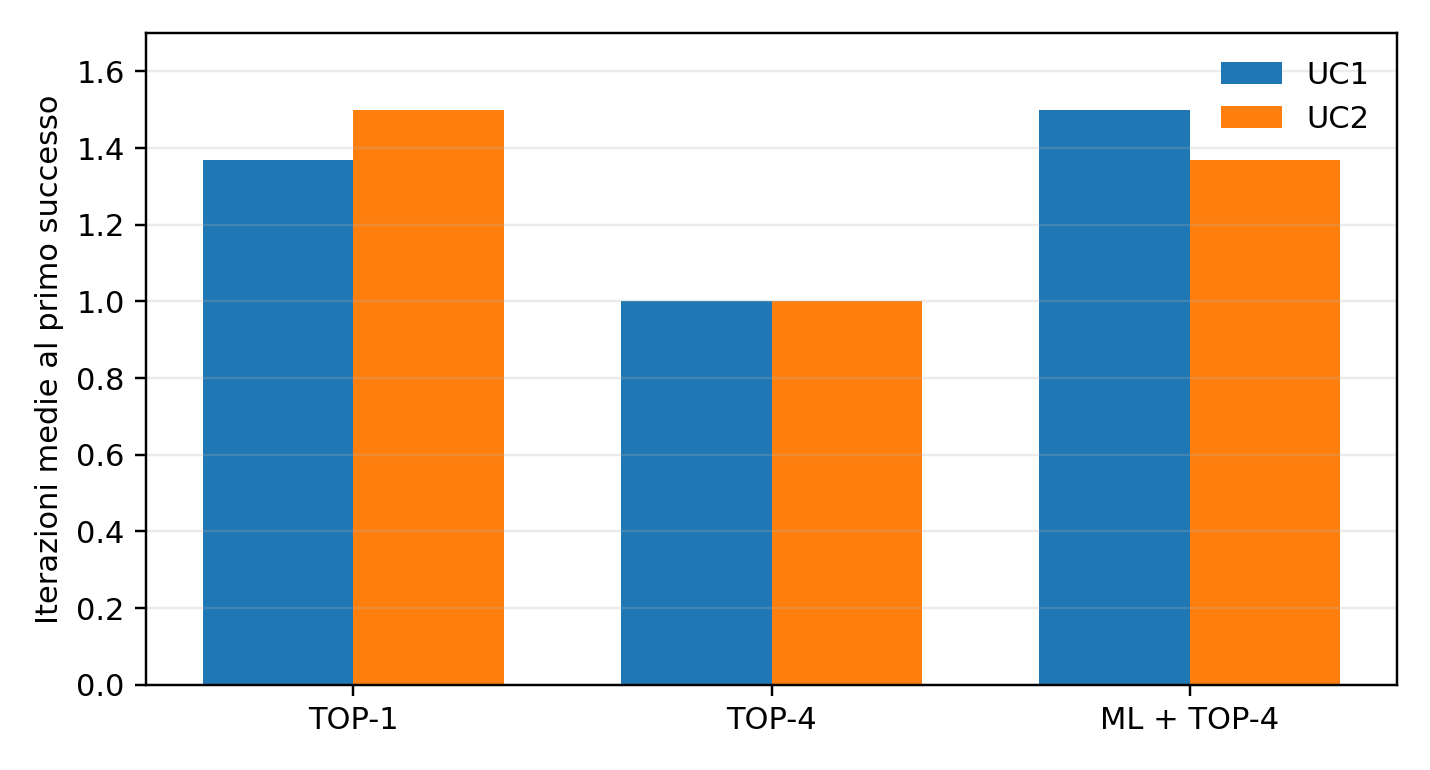
\includegraphics[width=0.85\textwidth,height=0.68\textheight,keepaspectratio]{finale_fig_5_1_iterazioni_primo_successo.png}

\caption{Numero medio di iterazioni al primo successo. L'ablazione mostra che il beneficio appartiene alla ricerca multi-candidato, non al classificatore.}\label{fig:finale_5_1}
\end{figure}

Nel perimetro dell'esperimento, l'interpretazione supportata dai dati è chiara: il classificatore è accurato, ma filtra alcuni istogrammi che TOP-4 avrebbe risolto direttamente. La prestazione predittiva è quindi reale, ma non è allineata all'obiettivo operativo. Si tratta di un risultato negativo rispetto all'ipotesi iniziale sul filtro, ma informativo sul piano metodologico: mostra perché un modello appreso debba essere confrontato con una baseline che utilizzi la stessa informazione e la stessa possibilità di verifica classica. Questo esito è coerente con la distinzione, presente anche nella letteratura recente sull'order finding rumoroso, fra riconoscibilità statistica dell'output e utilità operativa del post-processing \cite{skosana2021,yang2026,smolin2013}.

\subsection{Audit combinatorio: perché TOP-K può apparire molto robusto}\label{sec:finale_5_1_3}

L'istanza N=15 rende necessario un secondo controllo. Con otto bit di misura esistono 256 possibili valori; la procedura classica adottata restituisce fattori non banali per 63 di essi. Se gli esiti fossero uniformi, la probabilità che un singolo candidato sia utile sarebbe già 63/256=24.61\%. All'aumentare di K, la probabilità di includere almeno uno dei 63 valori utili cresce rapidamente anche in assenza di struttura quantistica. Per K=4 vale circa 67.94\%; per K=16 circa 99.07\%.

\begingroup
\small
\begin{table}[!htbp]
\centering
\small

\begin{tabular}{@{}
  >{\raggedright\arraybackslash}p{(\linewidth - 4\tabcolsep) * \real{0.0820}}
  >{\centering\arraybackslash}p{(\linewidth - 4\tabcolsep) * \real{0.4262}}
  >{\centering\arraybackslash}p{(\linewidth - 4\tabcolsep) * \real{0.4918}}@{}}
\toprule
\textbf{K} & \textbf{P(nessun esito utile)} & \textbf{P(almeno un esito utile)} \\
\midrule
1 & 75.39\% & 24.61\% \\
\addlinespace[0.3em]
2 & 56.76\% & 43.24\% \\
\addlinespace[0.3em]
4 & 32.06\% & 67.94\% \\
\addlinespace[0.3em]
16 & 0.93\% & 99.07\% \\
\bottomrule
\end{tabular}
\caption{Baseline combinatoria per una scelta di K celle senza informazione sulla distribuzione, data la specifica procedura di estrazione dei fattori.}\label{tab:finale_5_4}

\end{table}
\endgroup

\begin{figure}[H]
\centering
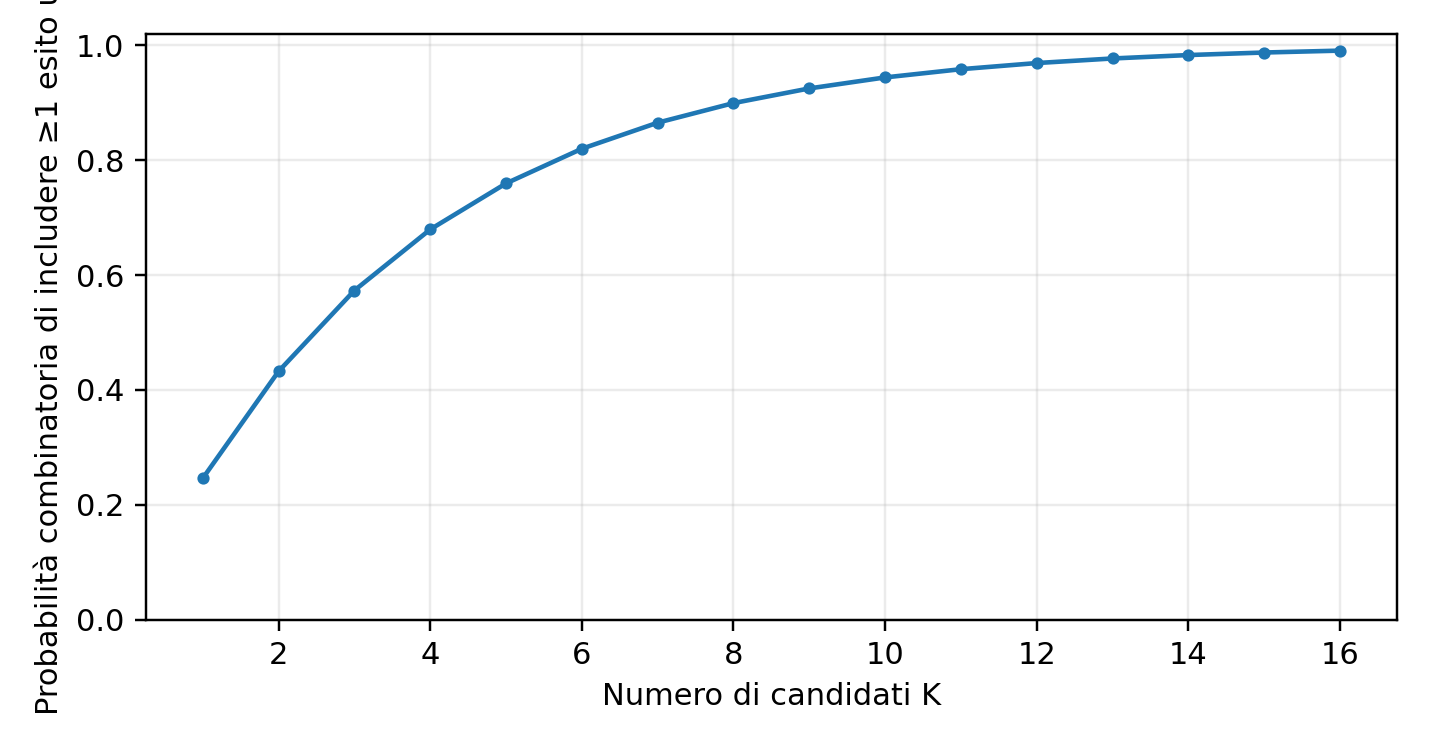
\includegraphics[width=0.75\textwidth,height=0.68\textheight,keepaspectratio]{finale_fig_5_2_baseline_combinatoria_topk.png}

\caption{Probabilità puramente combinatoria di includere almeno un esito utile fra i primi K candidati. Un elevato successo TOP-K non è, da solo, una misura di fedeltà quantistica.}\label{fig:finale_5_2}
\end{figure}

Questo controllo chiarisce anche il significato di TOP-16. Nei dataset rigenerati la regola TOP-16 produce 2 000 positivi e 0 negativi in entrambi gli scenari; non definisce quindi un problema di classificazione discriminante. Il risultato non implica che l'istogramma sia quasi ideale: riflette in larga misura la permissività combinatoria della verifica su questa piccola istanza.

\subsection{Struttura residua dell'istogramma e confronto con la ZNE}\label{sec:finale_5_1_4}\label{sec:parametri_mitigazione}

Per evitare di confondere il successo della procedura classica con la qualità della distribuzione, è stata misurata separatamente la massa sui quattro picchi QPE teorici \{0,64,128,192\}. L'indice descrittivo normalizzato f passa da 0.8036 a λ\_2q=10⁻³ a 0.0015 a λ\_2q=0.3. Il proxy di nessun evento Pauli sulle 224 porte CX decade molto più rapidamente: a λ\_2q=0.1 vale 2.65×10⁻¹⁰, mentre f è ancora 0.0421. I due oggetti non sono quindi intercambiabili: il proxy conta la probabilità di evitare una classe di eventi, mentre l'algoritmo può conservare informazione utile anche dopo alcuni errori.

\begingroup
\small
\begin{table}[!htbp]
\centering
\small

\begin{tabular}{@{}
  >{\raggedright\arraybackslash}p{(\linewidth - 4\tabcolsep) * \real{0.1356}}
  >{\centering\arraybackslash}p{(\linewidth - 4\tabcolsep) * \real{0.4068}}
  >{\centering\arraybackslash}p{(\linewidth - 4\tabcolsep) * \real{0.4576}}@{}}
\toprule
\textbf{$\lambda_{2q}$} & \textbf{Indice f sui picchi} & \textbf{Proxy nessun evento 2Q} \\
\midrule
10⁻³ & 0.8036 & 8.11×10⁻¹ \\
\addlinespace[0.3em]
5×10⁻³ & 0.7039 & 3.49×10⁻¹ \\
\addlinespace[0.3em]
10⁻² & 0.5938 & 1.21×10⁻¹ \\
\addlinespace[0.3em]
2×10⁻² & 0.4286 & 1.44×10⁻² \\
\addlinespace[0.3em]
5×10⁻² & 0.1688 & 2.14×10⁻⁵ \\
\addlinespace[0.3em]
10⁻¹ & 0.0421 & 2.65×10⁻¹⁰ \\
\addlinespace[0.3em]
2×10⁻¹ & 0.0047 & 6.32×10⁻²¹ \\
\addlinespace[0.3em]
3×10⁻¹ & 0.0015 & 7.47×10⁻³³ \\
\bottomrule
\end{tabular}
\caption{Struttura residua sui picchi QPE e proxy di nessun evento Pauli 2Q.}\label{tab:finale_5_5}\label{tab:frazione_coerente}

\par\medskip
\normalsize
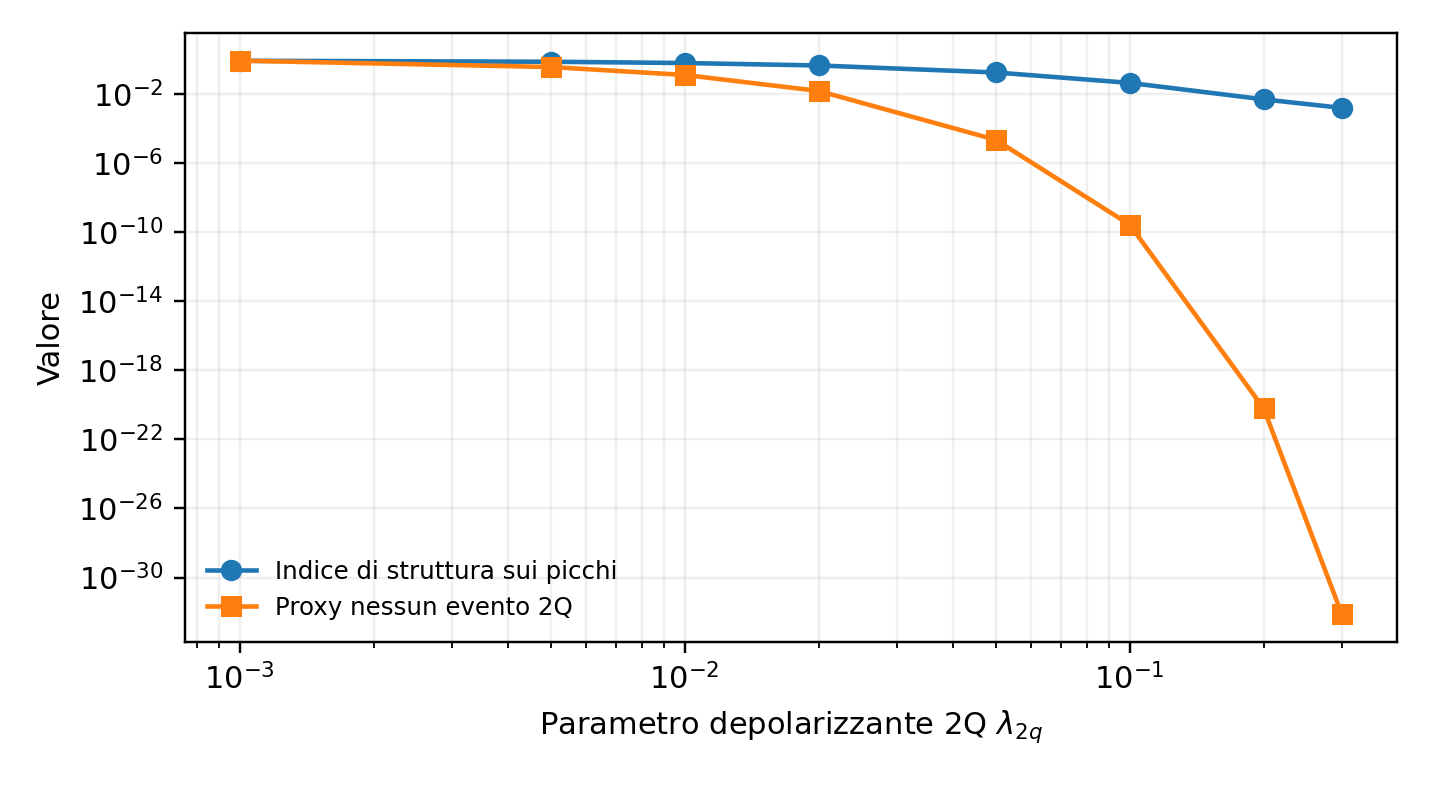
\includegraphics[width=0.70\textwidth,height=0.27\textheight,keepaspectratio]{finale_fig_5_3_struttura_picchi_proxy_2q.png}

\captionof{figure}{Il proxy moltiplicativo decade molto più rapidamente dell'indice che misura la struttura residua sui picchi QPE.}\label{fig:finale_5_3}\label{fig:frazione_coerente}
\end{table}
\endgroup

La Zero-Noise Extrapolation digitale, usata come confronto aggiuntivo nello scenario UC1, non riduce il numero di iterazioni e aumenta il costo di campionamento. ZNE-2 richiede in media 3 072 shot complessivi e ZNE-3 4 813, rispetto a 1 399 di TOP-1 e 1 024 di TOP-4. Poiché il protocollo scala i parametri depolarizzanti nel simulatore e non implementa gate folding su hardware, questo esito è locale al modello adottato e non costituisce una valutazione generale della ZNE. Il confronto è volutamente locale: la ZNE ha fondamenti generali consolidati, ma la sua efficacia dipende dalla realizzazione del noise scaling e dall'osservabile considerato \cite{temme2017,liBenjamin2017}. La tabella appaiata completa e il contratto della campagna sono conservati nell'Appendice~\ref{app:parametrica}.

Gli sweep su K, numero di shot, T1/T2, errore 1Q/2Q, readout e livello di ottimizzazione confermano che TOP-4 rimane molto efficace nell'istanza N=15 lungo gli intervalli esplorati. Tale robustezza non va però generalizzata: con 63 esiti accettabili su 256 e soli quattro picchi ideali, l'istanza offre condizioni combinatorie particolarmente favorevoli. Intervalli, griglie ed esiti per ciascuna famiglia sono riportati nelle Tabelle D.3--D.10 dell'Appendice~\ref{app:parametrica}.

La tabella va letta come mappa di stabilità locale, non come prova di insensibilità. In particolare, l'assenza di variazione osservata con 30 repliche non autorizza a concludere che readout, coerenza o livello di ottimizzazione siano irrilevanti in generale. Il risultato è specifico della piccola istanza N=15 e della sua struttura di picchi.

\par\medskip\noindent\rule{\linewidth}{0.6pt}\par\nopagebreak
{\small\setstretch{1.15}\noindent \textbf{Risposta a DR1.} La ricerca multi-candidato riduce in modo significativo il costo della fattorizzazione rispetto a TOP-1. Il classificatore considerato non aggiunge un beneficio rispetto alla stessa TOP-4 senza filtro, nonostante F1 e AUC elevate. Nel perimetro studiato, la complessità appresa è quindi non necessaria a valle dell'istogramma; il risultato utile è l'ablazione che identifica la vera sorgente del guadagno.\par}
\nopagebreak\noindent\rule{\linewidth}{0.6pt}\par\medskip

\section{DR2 - Correzione quantistica: dalla soppressione elementare alla soglia del surface code}\label{sec:finale_5_2}

La seconda domanda di ricerca riguarda un problema diverso: non come utilizzare meglio gli esiti già misurati, ma se la codifica possa ridurre la probabilità di errore dell'informazione logica durante la conservazione dello stato. La progressione sperimentale usa il codice a ripetizione come controllo elementare, il codice di Steane come primo codice capace di correggere un errore arbitrario su un qubit e il surface code per studiare il ruolo della distanza e della soglia.

\subsection{Codice a ripetizione: verifica della legge analitica}\label{sec:finale_5_2_1}\label{sec:repetition}

Per il codice a ripetizione a tre qubit, un fallimento logico si verifica quando almeno due qubit subiscono l'errore considerato. La probabilità teorica è

p\_L = 3p²(1-p) + p³ = 3p² - 2p³.

La simulazione Monte Carlo usa 20 000 campioni per punto e riproduce la curva analitica entro l'incertezza statistica, sia per la protezione da bit flip sia per il duale in base di Hadamard. A p=0.10 si osserva p\_L=0.0288±0.0012, contro 0.0280 teorico; a p=0.20 si osserva 0.1026±0.0021, contro 0.1040. Sotto p=0.5 il codice riduce l'errore da O(p) a O(p²); a p=0.5 si raggiunge il break-even. Il risultato ha valore soprattutto come validazione della pipeline di sindrome e decodifica: il codice protegge da una sola classe di errore per volta e non è una soluzione generale.

\subsection{Codice di Steane: soppressione quadratica e pseudo-soglia}\label{sec:finale_5_2_2}\label{sec:steane}

Nel codice di Steane \ensuremath{[[7,1,3]]} vengono prima verificati il code space e la corrispondenza sindrome-errore. La preparazione di \textbar0\_L⟩ produce sindrome nulla in 2 000 campioni; l'iniezione deterministica di X, Z e Y su ciascuno dei sette qubit copre 21 casi e restituisce sindromi distinte e coerenti con la lookup table.

La campagna quantitativa, con 200 000 campioni per punto, mostra p\_L∝p\^{}γ con pendenza log-log γ=1.94, in accordo con la soppressione quadratica attesa per un codice di distanza tre quando i fallimenti iniziano al secondo errore. Il confronto con il qubit fisico individua una pseudo-soglia intorno a p≈0.08: a p=0.01 si osserva p\_L=1.67×10⁻³, a p=0.05 p\_L=3.4×10⁻², mentre a p=0.10 p\_L=0.116 e la codifica non è più conveniente.

\begingroup
\small
\begin{table}[!htbp]
\centering
\small

\begin{tabular}{@{}
  >{\raggedright\arraybackslash}p{(\linewidth - 6\tabcolsep) * \real{0.1528}}
  >{\centering\arraybackslash}p{(\linewidth - 6\tabcolsep) * \real{0.2118}}
  >{\centering\arraybackslash}p{(\linewidth - 6\tabcolsep) * \real{0.2300}}
  >{\centering\arraybackslash}p{(\linewidth - 6\tabcolsep) * \real{0.4054}}@{}}
\toprule
\textbf{p fisico} & \textbf{$p_L$ osservato} & \textbf{Confronto con p} & \textbf{Interpretazione} \\
\midrule
0.01 & 1.67×10⁻³ & $p_L$ \textless{} p & soppressione marcata \\
\addlinespace[0.3em]
0.05 & 3.4×10⁻² & $p_L$ \textless{} p & codifica ancora conveniente \\
\addlinespace[0.3em]
0.10 & 0.116 & $p_L$ \textgreater{} p & oltre la pseudo-soglia \\
\bottomrule
\end{tabular}
\caption{Punti rappresentativi della campagna Steane.}\label{tab:finale_5_8}

\end{table}
\endgroup

La parola pseudo-soglia è essenziale. Nel modello implementato gli errori agiscono sui qubit dati e l'estrazione della sindrome è assunta ideale; non vengono simulate tutte le location di guasto di un protocollo fault-tolerant. L'intersezione p\_L=p caratterizza quindi questo specifico memory experiment, non la soglia fault-tolerant del codice in un'architettura completa.

\subsection{Surface code: comportamento di soglia e fit di scala}\label{sec:finale_5_2_3}\label{sec:surface_concetto}\label{sec:surface_risultati}

Il surface code introduce un parametro di scala reale: la distanza d. La campagna usa d=3,5,7,9, memorie nelle basi X e Z, rounds=d e rumore circuit-level. Sotto soglia, aumentando d deve diminuire p\_L; sopra soglia l'ordine delle curve si inverte. L'esperimento riproduce precisamente questo comportamento.

\begin{figure}[H]
\centering
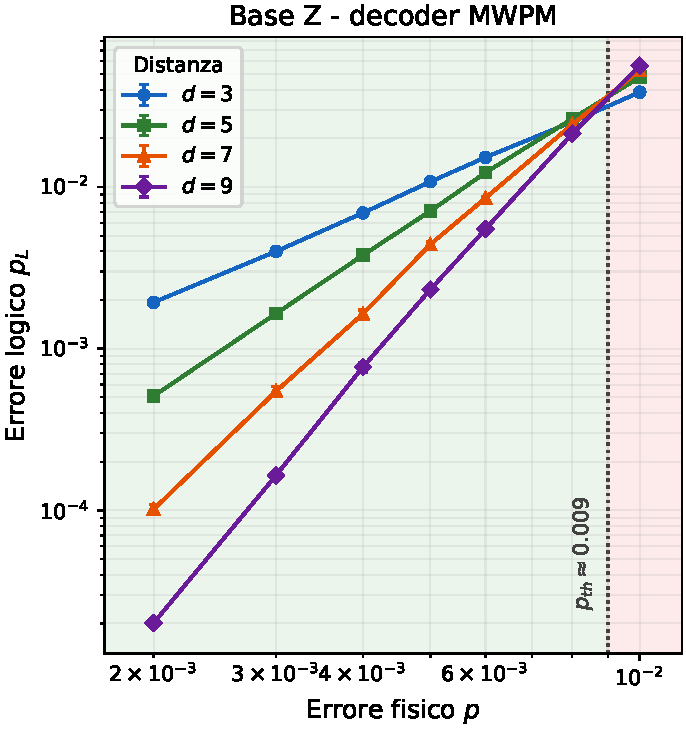
\includegraphics[width=0.49\textwidth]{finale_fig_5_4_surface_code_z.pdf}\hfill
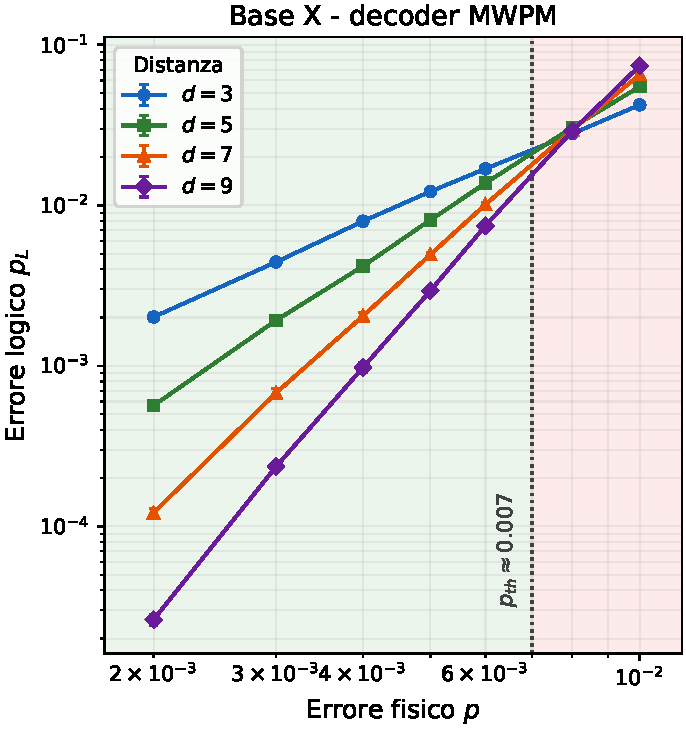
\includegraphics[width=0.49\textwidth]{finale_fig_5_4_surface_code_x.pdf}

\caption{Errore logico del surface code ruotato al variare dell'errore fisico e della distanza. Il grafico è ripreso dalla campagna M7 della tesi e mostra l'inversione dell'ordine delle curve sopra soglia.}\label{fig:finale_5_4}
\end{figure}

A p=2×10⁻³, nella memoria Z, p\_L scende da 1.94×10⁻³ a d=3 a 5.10×10⁻⁴ a d=5, 1.02×10⁻⁴ a d=7 e 2.01×10⁻⁵ a d=9. Il miglioramento è quindi progressivo e, fra d=5 e d=9, compatibile con una riduzione circa geometrica. A p=10⁻² l'ordine si inverte: p\_L è circa 3.9\% a d=3 e 5.6\% a d=9. L'incrocio visuale si colloca intorno a 0.9\% in base Z e 0.7\% in base X.

Un fit nel regime sotto soglia usa la legge p\_L(d,p)=A(p/p\_th)\^{}\{⌊(d+1)/2⌋\}. Con i punti p≤6×10⁻³ restituisce p\_th=0.86\% in base Z e 0.81\% in base X, con residuo quadratico medio 0.08 in ln(p\_L). L'accordo fra fit e incrocio è un controllo interno, ma non rende universale la soglia: essa dipende dal circuito di memoria, dal modello di rumore e dal decoder MWPM utilizzati. L'interpretazione del crossing e dello scaling con la distanza è coerente con la teoria del surface code e con dimostrazioni sperimentali recenti di soppressione logica sotto soglia \cite{fowler2012,googleQECBelowThreshold2025,googleSurfaceCode2023,dennis2002topological}.

\begingroup
\small
\begin{table}[!htbp]
\centering
\small

\begin{tabular}{@{}
  >{\raggedright\arraybackslash}p{(\linewidth - 8\tabcolsep) * \real{0.1129}}
  >{\centering\arraybackslash}p{(\linewidth - 8\tabcolsep) * \real{0.2047}}
  >{\centering\arraybackslash}p{(\linewidth - 8\tabcolsep) * \real{0.1340}}
  >{\centering\arraybackslash}p{(\linewidth - 8\tabcolsep) * \real{0.1613}}
  >{\centering\arraybackslash}p{(\linewidth - 8\tabcolsep) * \real{0.3871}}@{}}
\toprule
\textbf{Base} & \textbf{Stima da incrocio} & \textbf{Fit $p_{\mathrm{th}}$} & \textbf{A} & \textbf{Nota} \\
\midrule
Z & ≈0.9\% & 0.86\% & 3.5×10⁻² & fit sui punti p≤6×10⁻³ \\
\addlinespace[0.3em]
X & ≈0.7\% & 0.81\% & 3.4×10⁻² & stesso protocollo \\
\bottomrule
\end{tabular}
\caption{Stime della soglia del surface code nel modello adottato.}\label{tab:finale_5_9}

\end{table}
\endgroup

\subsection{Implicazione ingegneristica: distanza e overhead della memoria}\label{sec:finale_5_2_4}

Invertendo il fit è possibile stimare, nel solo modello di memoria utilizzato, quale distanza sarebbe necessaria per raggiungere un dato p\_L. Per un surface code ruotato il numero di qubit fisici per qubit logico è approssimativamente 2d²-1. Il risultato quantifica il valore della qualità dei gate: dimezzare l'errore fisico da 2×10⁻³ a 10⁻³ riduce sensibilmente la distanza richiesta.

\begingroup
\small
\begin{table}[!htbp]
\centering
\small

\begin{tabular}{@{}
  >{\raggedright\arraybackslash}p{(\linewidth - 8\tabcolsep) * \real{0.2212}}
  >{\centering\arraybackslash}p{(\linewidth - 8\tabcolsep) * \real{0.2120}}
  >{\centering\arraybackslash}p{(\linewidth - 8\tabcolsep) * \real{0.1935}}
  >{\centering\arraybackslash}p{(\linewidth - 8\tabcolsep) * \real{0.1797}}
  >{\centering\arraybackslash}p{(\linewidth - 8\tabcolsep) * \real{0.1935}}@{}}
\toprule
\textbf{$p_L$ richiesto} & \textbf{d a p=2×10⁻³} & \textbf{qubit fisici} & \textbf{d a p=10⁻³} & \textbf{qubit fisici} \\
\midrule
10⁻⁴ & 9 & 161 & 5 & 49 \\
\addlinespace[0.3em]
10⁻⁶ & 15 & 449 & 9 & 161 \\
\addlinespace[0.3em]
10⁻⁹ & 23 & 1 057 & 17 & 577 \\
\addlinespace[0.3em]
10⁻¹² & 33 & 2 177 & 23 & 1 057 \\
\bottomrule
\end{tabular}
\caption{Estrapolazione del fit di memoria. Per distanze superiori a quelle simulate i valori sono stime di modello, non misure hardware.}\label{tab:finale_5_10}

\end{table}
\endgroup

Questa tabella non è una stima del costo di Shor fault-tolerant. Proteggere una memoria e realizzare un gate logico non sono lo stesso problema: un'esecuzione completa richiederebbe operazioni logiche, cicli di sindrome, routing, feed-forward, gestione delle operazioni non-Clifford e correlazioni residue. Il risultato utile è più circoscritto: sotto soglia, la qualità fisica del dispositivo si traduce direttamente in overhead di codifica.

\subsection{Controllo oltre il modello Pauli}\label{sec:finale_5_2_5}\label{sec:oltre_pauli}

Un controllo full-state a d=3 confronta il modello Pauli con sovrarotazioni coerenti. A p=3×10⁻² si osservano meno flip grezzi sotto sovrarotazione, 0.237 contro 0.262, ma un errore MWPM leggermente maggiore, 0.0789 contro 0.0767, pari a circa +2.9\%. Per il decoder ibrido, le differenze di guadagno fra rumore Pauli e coerente sono dell'ordine di una deviazione standard e non risultano statisticamente risolte. Questo controllo non dimostra equivalenza fra canali: mostra che, nel regime studiato, il risultato appreso discusso più avanti non dipende semplicemente dal carattere non-Pauli del rumore.

\par\medskip\noindent\rule{\linewidth}{0.6pt}\par\nopagebreak
{\small\setstretch{1.15}\noindent \textbf{Risposta a DR2.} I tre livelli di codifica mostrano una progressione coerente: il repetition code riproduce la legge analitica di soppressione, Steane riduce l'errore da O(p) a O(p²) nel modello con sindrome ideale, e il surface code mostra un comportamento di soglia con soppressione crescente all'aumentare della distanza sotto p\_th. Le soglie e le stime di overhead restano proprietà del memory experiment adottato e non possono essere trasferite direttamente a Shor fault-tolerant.\par}
\nopagebreak\noindent\rule{\linewidth}{0.6pt}\par\medskip

\section{DR3 - Decoder analitici, appresi e ibridi}\label{sec:finale_5_3}\label{sec:decodifica_appresa}

La terza domanda di ricerca verifica dove il machine learning possa aggiungere informazione a un decoder analitico. È la parte più delicata della campagna, perché una rete può apparire vantaggiosa semplicemente se la baseline scelta è debole. Per questo il percorso sperimentale non si arresta al confronto rete-MWPM: vengono verificati il costo in dati, il rumore correlato, l'uso della rete come validatore, un decoder ibrido residuale, la robustezza alla mis-calibrazione, il confronto con BP+OSD, la non additività dei guadagni e la trasferibilità fra profili simulati.

\subsection{Sostituire MWPM con una rete: risultato negativo a modello corretto}\label{sec:finale_5_3_1}

Quando MWPM riceve il detector error model corretto, la rete densa non lo supera con significatività statistica in nessuna delle quattordici configurazioni iniziali, costituite da d=3 e d=5 su sette valori di p. A d=3 la rete si avvicina progressivamente al matching; a d=5 resta invece nettamente peggiore. Un esperimento dedicato varia soltanto la numerosità del training set a d=3, p=3×10⁻³: il rapporto fra errore MWPM e errore della rete cresce da 0.50 con 2.5×10⁴ campioni a 1.02 con 8×10⁵. Nell'ultimo punto, p\_L è 3.98×10⁻³ per la rete e 4.04×10⁻³ per MWPM, ma lo scarto vale soltanto 0.2 deviazioni standard e non è significativo.

Il dato più informativo non è quindi che la rete ``fallisca'', ma il costo per arrivare al pareggio: nell'architettura densa adottata servono circa 10⁵--10⁶ campioni soltanto per raggiungere MWPM a d=3. Aumentare il volume dei dati aiuta, ma non risolve il problema di scala quando la rappresentazione della sindrome cresce.

\subsection{Rumore correlato: quando la struttura del decoder diventa il collo di bottiglia}\label{sec:finale_5_3_2}

La situazione cambia introducendo un errore correlato fra qubit dati adiacenti, usato come modello elementare di crosstalk. L'errore fisico di base rimane p=3×10⁻³. A d=3, la rete appresa dai campioni supera MWPM in tutte e quattro le intensità considerate; a d=5 il quadro si inverte. Nel modello simulato, il risultato indica che una buona stima dei parametri del rumore non è sufficiente quando la struttura del decoder non rappresenta adeguatamente la classe di correlazioni osservata.

\begingroup
\small
\begin{table}[!htbp]
\centering
\small

\begin{tabular}{@{}
  >{\raggedright\arraybackslash}p{(\linewidth - 8\tabcolsep) * \real{0.0806}}
  >{\centering\arraybackslash}p{(\linewidth - 8\tabcolsep) * \real{0.1935}}
  >{\centering\arraybackslash}p{(\linewidth - 8\tabcolsep) * \real{0.2514}}
  >{\centering\arraybackslash}p{(\linewidth - 8\tabcolsep) * \real{0.3292}}
  >{\centering\arraybackslash}p{(\linewidth - 8\tabcolsep) * \real{0.1452}}@{}}
\toprule
\textbf{d} & \textbf{crosstalk} & \textbf{MWPM nominale} & \textbf{MWPM con crosstalk} & \textbf{Rete} \\
\midrule
3 & 0.005 & 0.03097 & 0.05656 & 0.02707 \\
\addlinespace[0.3em]
3 & 0.010 & 0.05966 & 0.08975 & 0.05012 \\
\addlinespace[0.3em]
3 & 0.020 & 0.11184 & 0.15107 & 0.09547 \\
\addlinespace[0.3em]
3 & 0.040 & 0.20806 & 0.25481 & 0.17568 \\
\addlinespace[0.7em]
5 & 0.005 & 0.03521 & 0.02796 & 0.08266 \\
\addlinespace[0.3em]
5 & 0.010 & 0.08655 & 0.06526 & 0.13957 \\
\addlinespace[0.3em]
5 & 0.020 & 0.19933 & 0.15662 & 0.28906 \\
\addlinespace[0.3em]
5 & 0.040 & 0.37458 & 0.32515 & 0.44634 \\
\bottomrule
\end{tabular}
\caption{Errore logico in presenza di crosstalk. ``MWPM con crosstalk'' usa un DEM che tenta di rappresentare il canale correlato; le etichette descrivono modelli simulati, non misure hardware.}\label{tab:finale_5_11}

\end{table}
\endgroup

\begin{figure}[H]
\centering
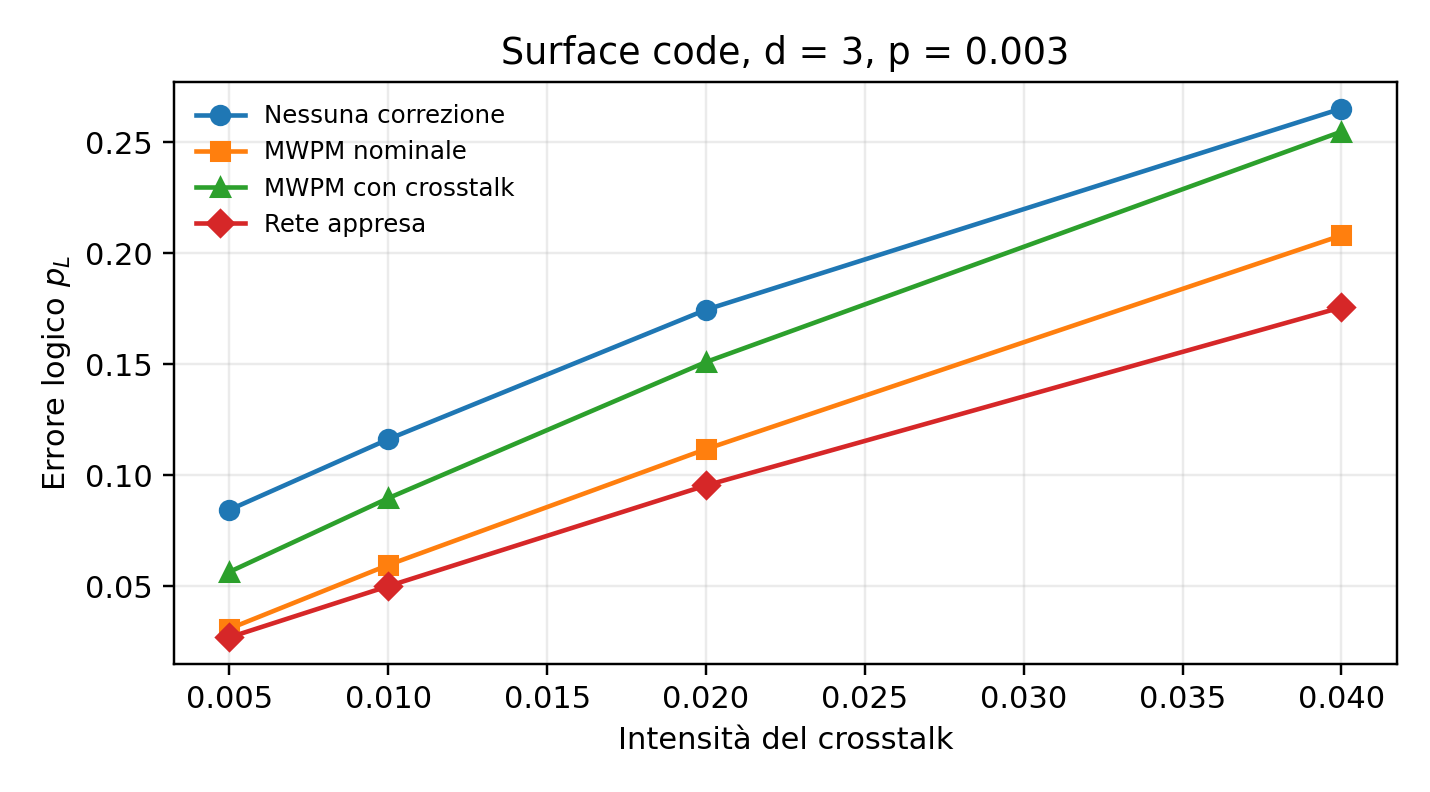
\includegraphics[width=0.85\textwidth,height=0.68\textheight,keepaspectratio]{finale_fig_5_5_decoder_crosstalk.png}

\caption{A distanza 3 la rete supera il matching nel regime di crosstalk simulato; il vantaggio non si trasferisce automaticamente a distanza 5.}\label{fig:finale_5_5}
\end{figure}

Un esito controintuitivo è che fornire a MWPM un modello che include il crosstalk non migliora sempre la decodifica. A d=3 e crosstalk 0.005, l'errore passa da 0.03097 con modello nominale a 0.05656 con il modello che tenta di includere il crosstalk. Nel modello adottato, questo comportamento è coerente con un limite di rappresentazione: l'errore correlato può attivare più detection event e la decomposizione richiesta dal grafo del matching può diventare inadeguata. A d=5, invece, il modello che include il crosstalk torna a essere il migliore dei due matching. Il dato richiede quindi di distinguere fra accuratezza della stima del canale e rappresentabilità del canale nel decoder.

\subsection{Dalla sostituzione al correttore residuale}\label{sec:finale_5_3_3}

La rete viene quindi usata per un compito più circoscritto: riconoscere quando MWPM ha sbagliato. A d=3 e crosstalk 0.01, il segnale appreso discrimina i fallimenti del matching con AUC=0.941. Alla soglia più restrittiva vengono segnalati solo lo 0.59\% degli shot, ma l'85.9\% delle segnalazioni è corretto; la recall è 0.085. La distinzione fra precision e recall è importante: il modello non intercetta la maggioranza degli errori, ma identifica un piccolo sottoinsieme sufficientemente puro da rendere conveniente l'intervento.

\begingroup
\small
\begin{table}[!htbp]
\centering
\small

\begin{tabular}{@{}
  >{\raggedright\arraybackslash}p{(\linewidth - 6\tabcolsep) * \real{0.1875}}
  >{\centering\arraybackslash}p{(\linewidth - 6\tabcolsep) * \real{0.3750}}
  >{\centering\arraybackslash}p{(\linewidth - 6\tabcolsep) * \real{0.2500}}
  >{\centering\arraybackslash}p{(\linewidth - 6\tabcolsep) * \real{0.1875}}@{}}
\toprule
\textbf{Soglia} & \textbf{Shot segnalati} & \textbf{Precision} & \textbf{Recall} \\
\midrule
0.5 & 2.92\% & 0.664 & 0.324 \\
\addlinespace[0.3em]
0.3 & 1.54\% & 0.783 & 0.202 \\
\addlinespace[0.3em]
0.2 & 1.16\% & 0.825 & 0.160 \\
\addlinespace[0.3em]
0.1 & 0.59\% & 0.859 & 0.085 \\
\bottomrule
\end{tabular}
\caption{Capacità della rete di segnalare i fallimenti di MWPM a d=3 e crosstalk 0.01.}\label{tab:finale_5_12}

\end{table}
\endgroup

Il decoder ibrido applica quindi la decisione di MWPM e la inverte soltanto quando la probabilità stimata di errore supera una soglia scelta su validation. La soglia può anche corrispondere a non intervenire mai; in tal caso il metodo ricade su MWPM. Il confronto è appaiato sugli stessi shot e viene valutato con il test di McNemar.

\begingroup
\small
\begin{table}[!htbp]
\centering
\small

\begin{tabular}{@{}
  >{\raggedright\arraybackslash}p{(\linewidth - 10\tabcolsep) * \real{0.0833}}
  >{\centering\arraybackslash}p{(\linewidth - 10\tabcolsep) * \real{0.2000}}
  >{\centering\arraybackslash}p{(\linewidth - 10\tabcolsep) * \real{0.1500}}
  >{\centering\arraybackslash}p{(\linewidth - 10\tabcolsep) * \real{0.1587}}
  >{\centering\arraybackslash}p{(\linewidth - 10\tabcolsep) * \real{0.1500}}
  >{\centering\arraybackslash}p{(\linewidth - 10\tabcolsep) * \real{0.2580}}@{}}
\toprule
\textbf{d} & \textbf{crosstalk} & \textbf{MWPM} & \textbf{Rete sola} & \textbf{Ibrido} & \textbf{Riduzione relativa vs MWPM} \\
\midrule
3 & 0.005 & 0.03089 & 0.02680 & 0.02607 & 15.6\% \\
\addlinespace[0.3em]
3 & 0.010 & 0.05829 & 0.04917 & 0.04851 & 16.8\% \\
\addlinespace[0.3em]
3 & 0.020 & 0.11144 & 0.09248 & 0.09183 & 17.6\% \\
\addlinespace[0.3em]
3 & 0.040 & 0.20750 & 0.17615 & 0.17455 & 15.9\% \\
\addlinespace[0.7em]
5 & 0.005 & 0.03561 & 0.06311 & 0.03521 & 1.1\% \\
\addlinespace[0.3em]
5 & 0.010 & 0.08704 & 0.12874 & 0.08428 & 3.2\% \\
\addlinespace[0.3em]
5 & 0.020 & 0.20231 & 0.25198 & 0.19662 & 2.8\% \\
\addlinespace[0.3em]
5 & 0.040 & 0.37581 & 0.44182 & 0.37385 & 0.5\% \\
\bottomrule
\end{tabular}
\caption{Decoder ibrido. La colonna finale riporta la riduzione relativa ($p_L^{\mathrm{MWPM}}-p_L^{\mathrm{ibrido}}$)/$p_L^{\mathrm{MWPM}}$; è distinta dal rapporto di guadagno $p_L^{\mathrm{MWPM}}/p_L^{\mathrm{ibrido}}$ usato negli artefatti originari.}\label{tab:finale_5_13}\label{tab:neural_ibrido}

\end{table}
\endgroup

Questa distinzione è importante perché il rapporto di guadagno e la riduzione relativa dell'errore non esprimono la stessa percentuale. Nei dati a d=3 il rapporto G=p\_L\^{}MWPM/p\_L\^{}ibrido varia fra circa 1.185 e 1.213, cioè un eccesso del 18--21\% rispetto a 1; espresso invece come riduzione relativa dell'errore, il miglioramento è 15.6--17.6\%. A d=5 la riduzione relativa è 0.5--3.2\%. Entrambe le metriche sono legittime, purché siano denominate e interpretate in modo distinto.

\subsection{Perché il vantaggio si riduce con la scala}\label{sec:finale_5_3_4}

A d=7 il correttore residuale tende ad astenersi anche quando il training set contiene molti fallimenti di MWPM. Il controllo E9 separa due variabili che in precedenza crescevano insieme: distanza del codice e numero di detector. Variando il numero di round a distanza fissa, il comportamento segue soprattutto la larghezza dell'ingresso. Con 336 detector il residuo si astiene sia a d=7 sia a d=5; con 120--144 detector interviene anche a distanza 7 quando dispone di un numero sufficiente di esempi. La matrice completa, con round, detector ed esempi positivi, è riportata nella Tabella E.6 dell'Appendice~\ref{app:decodifica}.

Un secondo controllo, E12, mostra che il problema non è soltanto la soglia di decisione. Con 336 detector l'AUC resta fra 0.57 e 0.77, quindi la rete conserva capacità di ranking; tuttavia persino una soglia oracolo scelta sul test produce un guadagno di circa 1.000. Perché invertire una decisione di MWPM sia vantaggioso, più della metà degli shot selezionati deve essere realmente errata: con input molto ampi la discriminazione non concentra abbastanza i fallimenti da superare questa soglia di precisione. Il risultato suggerisce quindi un limite legato anche alla rappresentazione e alla scala dell'architettura, non soltanto alla calibrazione statistica della soglia.

\subsection{Una baseline analitica più forte: BP+OSD}\label{sec:finale_5_3_5}

Il controllo più severo consiste nel sostituire MWPM con un decoder analitico più espressivo nel modello considerato, BP+OSD \cite{roffe2020,panteleev2021}. Entrambi i decoder analitici ricevono lo stesso modello nominale, privo di crosstalk, così la differenza dipende dalla regola di decodifica e non da un vantaggio informativo. Il risultato modifica l'interpretazione del confronto: a modello corretto BP+OSD sfrutta meglio la struttura disponibile; quando il crosstalk rende incompleta la descrizione nominale, il suo vantaggio si erode mentre quello del residuo appreso cresce.

\begingroup
\scriptsize
\begin{table}[!htbp]
\centering
\small

\begin{tabular}{@{}
  >{\raggedright\arraybackslash}p{(\linewidth - 10\tabcolsep) * \real{0.0909}}
  >{\centering\arraybackslash}p{(\linewidth - 10\tabcolsep) * \real{0.2182}}
  >{\centering\arraybackslash}p{(\linewidth - 10\tabcolsep) * \real{0.1636}}
  >{\centering\arraybackslash}p{(\linewidth - 10\tabcolsep) * \real{0.1636}}
  >{\centering\arraybackslash}p{(\linewidth - 10\tabcolsep) * \real{0.1818}}
  >{\centering\arraybackslash}p{(\linewidth - 10\tabcolsep) * \real{0.1818}}@{}}
\toprule
\textbf{d} & \textbf{crosstalk} & \textbf{MWPM} & \textbf{BP+OSD} & \textbf{$G_{\mathrm{BP+OSD}}$} & \textbf{$G_{\mathrm{ibrido}}$} \\
\midrule
3 & 0 & 0.00428 & 0.00374 & 1.146 & 0.993 \\
\addlinespace[0.3em]
3 & 0.005 & 0.03193 & 0.03286 & 0.972 & 1.185 \\
\addlinespace[0.3em]
3 & 0.010 & 0.05912 & 0.06034 & 0.980 & 1.202 \\
\addlinespace[0.3em]
3 & 0.020 & 0.11176 & 0.11340 & 0.986 & 1.213 \\
\addlinespace[0.3em]
3 & 0.040 & 0.20811 & 0.20826 & 0.999 & 1.189 \\
\addlinespace[0.7em]
5 & 0 & 0.00192 & 0.00143 & 1.339 & 1.000 \\
\addlinespace[0.3em]
5 & 0.005 & 0.03565 & 0.02807 & 1.270 & 1.011 \\
\addlinespace[0.3em]
5 & 0.010 & 0.08638 & 0.07348 & 1.176 & 1.033 \\
\addlinespace[0.3em]
5 & 0.020 & 0.19998 & 0.18288 & 1.094 & 1.029 \\
\addlinespace[0.3em]
5 & 0.040 & 0.37561 & 0.36788 & 1.021 & 1.005 \\
\bottomrule
\end{tabular}
\caption{Confronto con BP+OSD. G è il rapporto $p_L^{\mathrm{MWPM}}/p_L^{\mathrm{metodo}}$; G\textgreater1 indica errore inferiore a MWPM.}\label{tab:finale_5_15}

\end{table}
\endgroup

\begin{figure}[H]
\centering
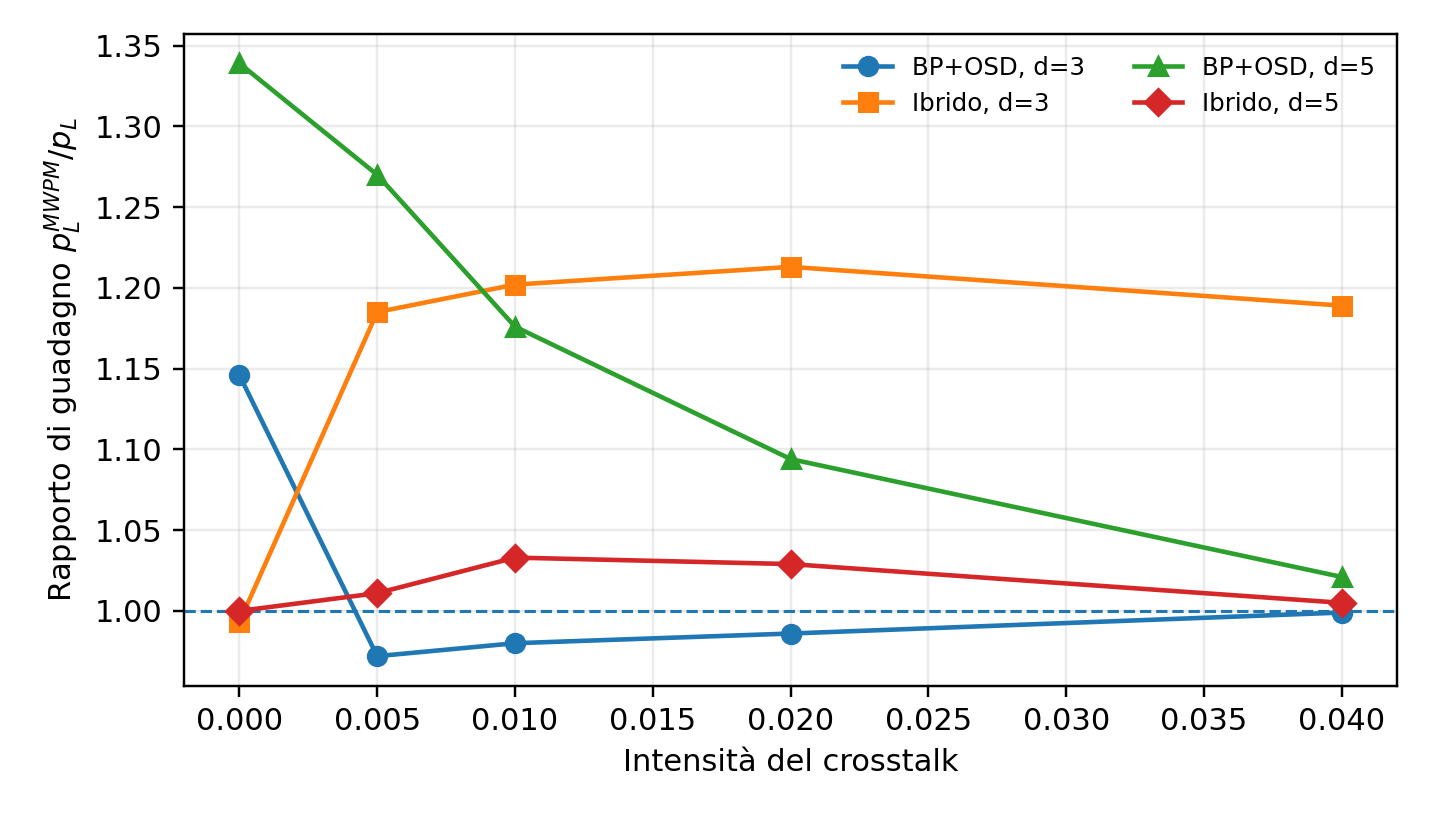
\includegraphics[width=0.85\textwidth,height=0.68\textheight,keepaspectratio]{finale_fig_5_6_decoder_bposd_ibrido.png}

\caption{Due sorgenti di guadagno: BP+OSD sfrutta meglio un modello rappresentabile; il residuo appreso recupera parte della struttura che il modello nominale non rappresenta.}\label{fig:finale_5_6}
\end{figure}

Nel caso senza crosstalk, a d=5 BP+OSD porta p\_L da 0.00192 a 0.00143: il rapporto di guadagno è 1.339, mentre la riduzione relativa dell'errore è 25.5\%. Con crosstalk 0.005 la riduzione relativa è 21.3\%; a 0.04 scende a circa 2.1\%. A d=3 il quadro opposto è evidente: appena compare il crosstalk, BP+OSD non supera più MWPM, mentre il residuo appreso mantiene un rapporto di guadagno fra 1.185 e 1.213. Ne consegue che il valore del machine learning va misurato contro il miglior decoder analitico plausibile nel regime considerato, non contro una baseline scelta per convenzione. Il confronto con decoder analitici più forti è essenziale per non attribuire al machine learning un margine dovuto soltanto a una baseline subottimale \cite{roffe2020,panteleev2021}.

\subsection{I guadagni sono additivi? Controlli E8--E11}\label{sec:finale_5_3_6}

Se BP+OSD e il residuo appreso agissero su errori indipendenti, il loro guadagno potrebbe essere moltiplicativo. E8 mette direttamente alla prova questa ipotesi costruendo il residuo sopra BP+OSD. Il combinato non raggiunge il prodotto previsto quando entrambi i componenti possiedono un guadagno reale; a distanza 5 lo scarto dal prodotto è sempre negativo, fra -0.007 e -0.027, e il residuo migliora BP+OSD in modo significativo in una sola configurazione, di circa l'1\%. Il combinato tende quindi a eguagliare il migliore dei due metodi, non a moltiplicarne i benefici. Le matrici complete di E8 ed E10 sono riportate nelle Tabelle E.10 ed E.11 dell'Appendice~\ref{app:decodifica}.

E10 chiarisce la ragione. In presenza di crosstalk, rete sola, MWPM+residuo e BP+OSD+residuo convergono entro circa 0.9--2.0\% l'uno dall'altro pur partendo da decoder differenti. Per crosstalk 0.01, ad esempio, i tre errori sono 0.04965, 0.04885 e 0.04982. Il risultato è compatibile con un pavimento comune associato all'informazione estraibile dalla sindrome nel modello adottato. E11 controlla che tale pavimento non sia semplicemente il limite della rete densa (128,64): una rete circa quaranta volte più grande raggiunge praticamente lo stesso livello, mentre una tabella empirica non parametrica non lo supera. Il dato non dimostra un limite informativo assoluto, ma rende poco plausibile che il risultato sia un artefatto della capacità del solo MLP utilizzato.

\subsection{Mis-calibrazione e trasferimento fra profili simulati}\label{sec:finale_5_3_7}

Due controlli delimitano ulteriormente il risultato. E6 perturba il rapporto fra errore di misura ed errore di gate nel modello fornito a MWPM. Il matching risulta robusto: errori di calibrazione anche molto ampi modificano in genere p\_L dell'ordine dell'1--3\%; soltanto a d=5 e con errore di misura sovrastimato del 900\% il costo sale di circa il 20\%. La rete non supera MWPM in nessuna delle dodici configurazioni. Nel perimetro studiato, il dato è quindi coerente con l'ipotesi che il margine appreso richieda un disallineamento strutturale, cioè una classe di correlazioni che il decoder non rappresenta, e non una semplice mis-calibrazione parametrica.

E5 valuta invece il trasferimento fra quattro intensità simulate di crosstalk. Tutte le dodici combinazioni fuori diagonale mantengono un vantaggio su MWPM e il costo medio del trasferimento, rispetto all'addestramento sul profilo di test, è circa 1.6\%. Il risultato mostra trasferibilità fra profili di intensità dello stesso modello simulato e della stessa geometria di codice; non dimostra trasferimento fra dispositivi fisici differenti o fra famiglie di rumore diverse. La matrice completa dei sedici incroci, insieme al confronto MWPM, è riportata nella Tabella~\ref{tab:neural_trasferimento} dell'Appendice~\ref{app:decodifica}.

Il trasferimento non elimina il problema di generalizzazione alla scala. La stessa architettura che si trasferisce bene fra intensità di crosstalk perde infatti efficacia quando aumenta il numero di detector. I due risultati non sono contraddittori: il primo riguarda la stabilità della regola appresa rispetto all'intensità di un meccanismo già rappresentato nei dati; il secondo riguarda la capacità del modello di rappresentare una sindrome di dimensione crescente. Questo limite di scala è coerente con la letteratura sui decoder neurali, che ricorre a architetture strutturate e dataset molto più ampi quando cresce la distanza del codice \cite{alphaqubit2024,torlaiMelko2017,yan2026}.

\subsection{Oltre il surface code: il Gross code nel modello code-capacity}\label{sec:finale_5_3_8}

Le sezioni precedenti confrontano decoder diversi sullo stesso codice. Il confronto esplorativo M16 cambia invece il codice: il Gross code \ensuremath{[[144,12,12]]} \cite{bravyi2024} viene messo a confronto con 12 patch indipendenti di surface code, che proteggono lo stesso numero di qubit logici, nel modello code-capacity descritto nella Sezione~\ref{sec:finale_3_5_4}. Prima dei confronti sono stati superati i controlli di costruzione: parametri \(n\), \(k\) e ranghi delle matrici coincidono con quelli pubblicati, la ricerca della distanza ritrova 12 per il Gross code e i valori attesi per gli altri quattro codici della famiglia e per il surface code, e nessuna correzione viola la sindrome in alcuna corsa. Sul surface code MWPM e BP+OSD coincidono entro l'incertezza, per cui il riferimento non è penalizzato dal proprio decoder.

\paragraph{Il decoder conta quanto il codice.} Nelle prime corse il Gross code, decodificato con BP+OSD ad aggiornamento parallelo dei messaggi, risultava peggiore di 12 patch a distanza 9 per \(q \le 1\%\). Uno sweep di dodici varianti del decoder sugli stessi shot ha mostrato che la sola schedulazione seriale riduce il fallimento logico di un ordine di grandezza o più a \(q = 1\)--2\% e di circa 2.5 volte a 3\%, con p di McNemar compresi fra 10⁻⁹ e 10⁻¹⁵⁰. Un secondo sweep attorno alla nuova configurazione non ha trovato varianti che la migliorassero di oltre il 10\%: a \(q = 1\%\) nove decoder diversi sbagliano esattamente gli stessi cinque shot su quattro milioni, segno che il margine residuo appartiene al codice più che alla regola di decodifica. La Tabella~\ref{tab:finale_5_gross_fw} mostra la causa: il decoder parallelo falliva già con tre errori, pur avendo il codice distanza 12; quello seriale non fallisce mai con meno di sei.

\begin{table}[!htbp]
\centering
\small

\begin{tabular}{@{}rcccc@{}}
\toprule
\(w\) & Gross, parallelo & Gross, seriale & surface \(d=9\) & surface \(d=11\) \\
\midrule
3 & \(1.9\times10^{-4}\) & 0 & 0 & 0 \\
\addlinespace[0.3em]
4 & \(8.4\times10^{-4}\) & 0 & 0 & 0 \\
\addlinespace[0.3em]
5 & \(2.0\times10^{-3}\) & 0 & \(2.8\times10^{-3}\) & 0 \\
\addlinespace[0.3em]
6 & \(3.6\times10^{-3}\) & \(7.1\times10^{-5}\) & \(1.5\times10^{-2}\) & \(2.7\times10^{-4}\) \\
\addlinespace[0.3em]
7 & \(5.8\times10^{-3}\) & \(5.4\times10^{-4}\) & \(4.1\times10^{-2}\) & \(1.7\times10^{-3}\) \\
\addlinespace[0.3em]
8 & \(8.9\times10^{-3}\) & \(2.7\times10^{-3}\) & \(8.7\times10^{-2}\) & \(6.1\times10^{-3}\) \\
\bottomrule
\end{tabular}
\caption{Probabilità di fallimento con esattamente \(w\) errori, \(f(w)\), fino a \(2\times10^{6}\) prove per peso. Per il Gross code seriale i pesi fino a 5 sono enumerati in modo esaustivo; per il surface code MWPM corregge per costruzione ogni errore di peso \(\le (d-1)/2\).}\label{tab:finale_5_gross_fw}

\end{table}

Lo zero del decoder seriale fino a peso 5 non è una stima: tutte le 498 685 189 configurazioni di errore di peso compreso fra 0 e 5 sono state decodificate senza alcun fallimento. Il decoder raggiunge quindi la capacità di correzione garantita dalla distanza, \(\lfloor(12-1)/2\rfloor = 5\). Un'analisi dei fallimenti ne chiarisce il meccanismo: nelle configurazioni parallele peggiori l'89--98\% degli errori nasce quando la belief propagation non converge e l'OSD, guidato da stime di probabilità fuorvianti, sceglie la correzione sbagliata. La schedulazione seriale converge molto più spesso (non convergenza 0.07\% contro 0.77\% a \(q = 2\%\)) e lascia all'OSD pochissimi casi. A \(q = 1\%\) il fallimento del blocco scende così da circa \(9.8\times10^{-5}\) a \(1.0\times10^{-6}\), circa cento volte.

\paragraph{Confronto con il surface code.} La Tabella~\ref{tab:finale_5_gross_confronto} riporta il confronto finale con il decoder seriale. Per \(q \le 2\%\) i valori derivano dalla decomposizione per peso, validata da due controlli diretti: per il Gross code a \(q = 1\%\) la simulazione diretta dà \(9.4\times10^{-7}\) (94 fallimenti su 10⁸ shot) contro \(1.01\times10^{-6}\) ricostruito, scarto del 7\%; per il surface code a distanza 13 dà \(1.350\times10^{-7}\) (135 su 10⁹) contro \(1.357\times10^{-7}\), scarto dello 0.5\%. Per \(q \ge 3\%\) i valori provengono da simulazione diretta.

\begin{table}[!htbp]
\centering
\small

\begin{tabular}{@{}lcccl@{}}
\toprule
\(q\) & Gross (144) & \(12\times d{=}11\) (1452) & \(12\times d{=}13\) (2028) & Esito rispetto a \(d=13\) \\
\midrule
0.2\% & \(5.3\times10^{-11}\) & \(8.4\times10^{-10}\) & \(2.3\times10^{-11}\) & peggiore \\
\addlinespace[0.3em]
0.3\% & \(6.2\times10^{-10}\) & \(9.4\times10^{-9}\) & \(3.9\times10^{-10}\) & peggiore \\
\addlinespace[0.3em]
0.5\% & \(1.39\times10^{-8}\) & \(1.95\times10^{-7}\) & \(1.35\times10^{-8}\) & compatibile \\
\addlinespace[0.3em]
0.75\% & \(1.68\times10^{-7}\) & \(2.1\times10^{-6}\) & \(2.2\times10^{-7}\) & migliore \\
\addlinespace[0.3em]
1\% & \(1.01\times10^{-6}\) & \(1.15\times10^{-5}\) & \(1.63\times10^{-6}\) & migliore \\
\addlinespace[0.3em]
2\% & \(8.4\times10^{-5}\) & \(6.2\times10^{-4}\) & \(1.77\times10^{-4}\) & migliore \\
\addlinespace[0.3em]
3\% & \(1.0\times10^{-3}\) & \(5.7\times10^{-3}\) & \(2.8\times10^{-3}\) & migliore \\
\addlinespace[0.3em]
5\% & \(2.8\times10^{-2}\) & \(8.0\times10^{-2}\) & \(5.2\times10^{-2}\) & migliore \\
\bottomrule
\end{tabular}
\caption{Probabilità che almeno uno dei 12 qubit logici fallisca, nel modello code-capacity. Fra parentesi i qubit di dato. ``Migliore'' e ``peggiore'' richiedono intervalli al 95\% non sovrapposti.}\label{tab:finale_5_gross_confronto}

\end{table}

Il Gross code protegge i 12 qubit logici meglio di 12 patch a distanza 11, che usano dieci volte i suoi qubit di dato, a tutti i livelli di rumore studiati, e meglio di 12 patch a distanza 13, con oltre quattordici volte i qubit di dato, per \(q \ge 0.75\%\). A rumore molto basso l'ordine si inverte rispetto alla distanza 13, come atteso: il Gross code fallisce a partire da sei errori, la patch a distanza 13 da sette, quindi il primo scala come \(q^6\) e la seconda come \(q^7\). In quel regime il Gross code si colloca fra le distanze 11 e 13, coerentemente con la sua distanza 12.

Lo stesso comportamento si ritrova nella famiglia bivariate bicycle, simulata con semi indipendenti che replicano anche il Gross code entro il 10\%. Tutti i codici con distanza almeno 10 battono le patch di surface code che usano lo stesso numero di qubit di dato o più. Il codice \ensuremath{[[288,12,18]]}, per \(q \ge 2\%\), batte 12 patch fino a distanza 17, che richiedono 3468 qubit di dato contro 288, con un margine di circa 250 volte a \(q = 2\%\) e 45 volte a 3\%. I codici \ensuremath{[[90,8,10]]} e \ensuremath{[[108,8,10]]}, con uguali \(k\) e \(d\), differiscono invece di circa cinque volte a \(q = 1\%\): la distanza non è l'unico fattore che conta. Tabelle complete, sweep del decoder e controlli sono nell'Appendice~\ref{app:gross}.

Il risultato va letto nel suo perimetro. Il modello code-capacity non include errori di misura né il circuito che estrae le sindromi; il confronto conta i soli qubit di dato, mentre includendo le ancille il Gross code usa 288 qubit e 12 patch a distanza 13 ne usano 4044; i numeri non sono confrontabili con le soglie circuit-level della Sezione~\ref{sec:finale_5_2_3} né con quelle pubblicate da IBM a livello di circuito. Il confronto mostra che struttura del codice e decoder determinano insieme il rapporto fra protezione e qubit impiegati; non costituisce una misura del miglioramento di Shor.

\par\medskip\noindent\rule{\linewidth}{0.6pt}\par\nopagebreak
{\small\setstretch{1.15}\noindent \textbf{Risposta a DR3.} Nel perimetro studiato, sostituire il decoder analitico con una rete non conviene. Il machine learning produce invece un beneficio come correttore residuale quando la sindrome contiene correlazioni non rappresentabili dalla struttura del decoder di riferimento. Il vantaggio è reale a piccola distanza, si riduce con la crescita dell'ingresso e deve essere confrontato con decoder analitici più forti come BP+OSD. I controlli mostrano inoltre che il guadagno appreso e quello analitico non sono semplicemente additivi. Cambiando codice, infine, il Gross code protegge 12 qubit logici con 144 qubit di dato meglio di 12 patch di surface code a distanza 13 per \(p \ge 0.75\%\) nel modello code-capacity, ma solo con un decoder adeguato: la schedulazione dei messaggi di BP+OSD sposta il suo errore logico di circa due ordini di grandezza.\par}
\nopagebreak\noindent\rule{\linewidth}{0.6pt}\par\medskip

\section{DR4 - Sensibilità dell'algoritmo di Shor al rumore per gate}\label{sec:finale_5_4}

La quarta domanda di ricerca è il punto di partenza concettuale dello studio: misura quanto rapidamente la specifica implementazione di Shor perde la capacità di fattorizzare al crescere dell'errore per gate, ed è questa fragilità a motivare le tre strategie di intervento. Viene presentata qui, dopo le campagne QEC, per mantenere l'ordine delle domande di ricerca. L'analisi collega il comportamento algoritmico al rumore senza identificare impropriamente le metriche QEC con gli errori di una computazione fault-tolerant. Nell'artefatto originario M8 il parametro veniva denominato p\_L; nella versione revisionata viene indicato p\_g per distinguerlo dal logical error rate dei memory experiment. p\_g è la probabilità totale di applicare un Pauli non identità dopo ciascun gate compilato incluso nel modello.

\subsection{Probabilità di fattorizzazione per singola misura}\label{sec:finale_5_4_1}\label{sec:risultati_logico}

Ogni punto aggrega 20 repliche da 4 096 shot, pari a 81 920 misure. In assenza di rumore il successo osservato è 0.7489, con IC Wilson 95\% {[}0.7459;0.7518{]}, coerente con il 75\% atteso dalla specifica procedura di post-processing. All'aumentare di p\_g la curva è compatibile con una funzione non crescente: a p\_g=0.01 il successo è 0.5651, a 0.02 è 0.4518 e a 0.05 scende a 0.2953.

\begingroup
\small
\begin{table}[!htbp]
\centering
\small

\begin{tabular}{@{}
  >{\raggedright\arraybackslash}p{(\linewidth - 4\tabcolsep) * \real{0.2564}}
  >{\centering\arraybackslash}p{(\linewidth - 4\tabcolsep) * \real{0.2821}}
  >{\centering\arraybackslash}p{(\linewidth - 4\tabcolsep) * \real{0.4615}}@{}}
\toprule
\textbf{$p_g$} & \textbf{$P_{\mathrm{success}}$} & \textbf{IC 95\%} \\
\midrule
0 & 0.7489 & {[}0.7459; 0.7518{]} \\
\addlinespace[0.3em]
10⁻⁴ & 0.7469 & {[}0.7439; 0.7498{]} \\
\addlinespace[0.3em]
5×10⁻⁴ & 0.7373 & {[}0.7343; 0.7403{]} \\
\addlinespace[0.3em]
10⁻³ & 0.7250 & {[}0.7219; 0.7280{]} \\
\addlinespace[0.3em]
1.7×10⁻³ & 0.7083 & {[}0.7051; 0.7114{]} \\
\addlinespace[0.3em]
2×10⁻³ & 0.6992 & {[}0.6961; 0.7024{]} \\
\addlinespace[0.3em]
5×10⁻³ & 0.6450 & {[}0.6417; 0.6483{]} \\
\addlinespace[0.3em]
10⁻² & 0.5651 & {[}0.5617; 0.5685{]} \\
\addlinespace[0.3em]
2×10⁻² & 0.4518 & {[}0.4484; 0.4552{]} \\
\addlinespace[0.3em]
5×10⁻² & 0.2953 & {[}0.2921; 0.2984{]} \\
\addlinespace[0.3em]
10⁻¹ & 0.2503 & {[}0.2474; 0.2533{]} \\
\addlinespace[0.3em]
2×10⁻¹ & 0.2441 & {[}0.2412; 0.2471{]} \\
\addlinespace[0.3em]
5×10⁻¹ & 0.2459 & {[}0.2430; 0.2489{]} \\
\bottomrule
\end{tabular}
\caption{Sensibilità M8: probabilità di ricavare i fattori per singola misura.}\label{tab:finale_5_19}\label{tab:m8_griglia_completa}

\end{table}
\endgroup

\begin{figure}[H]
\centering
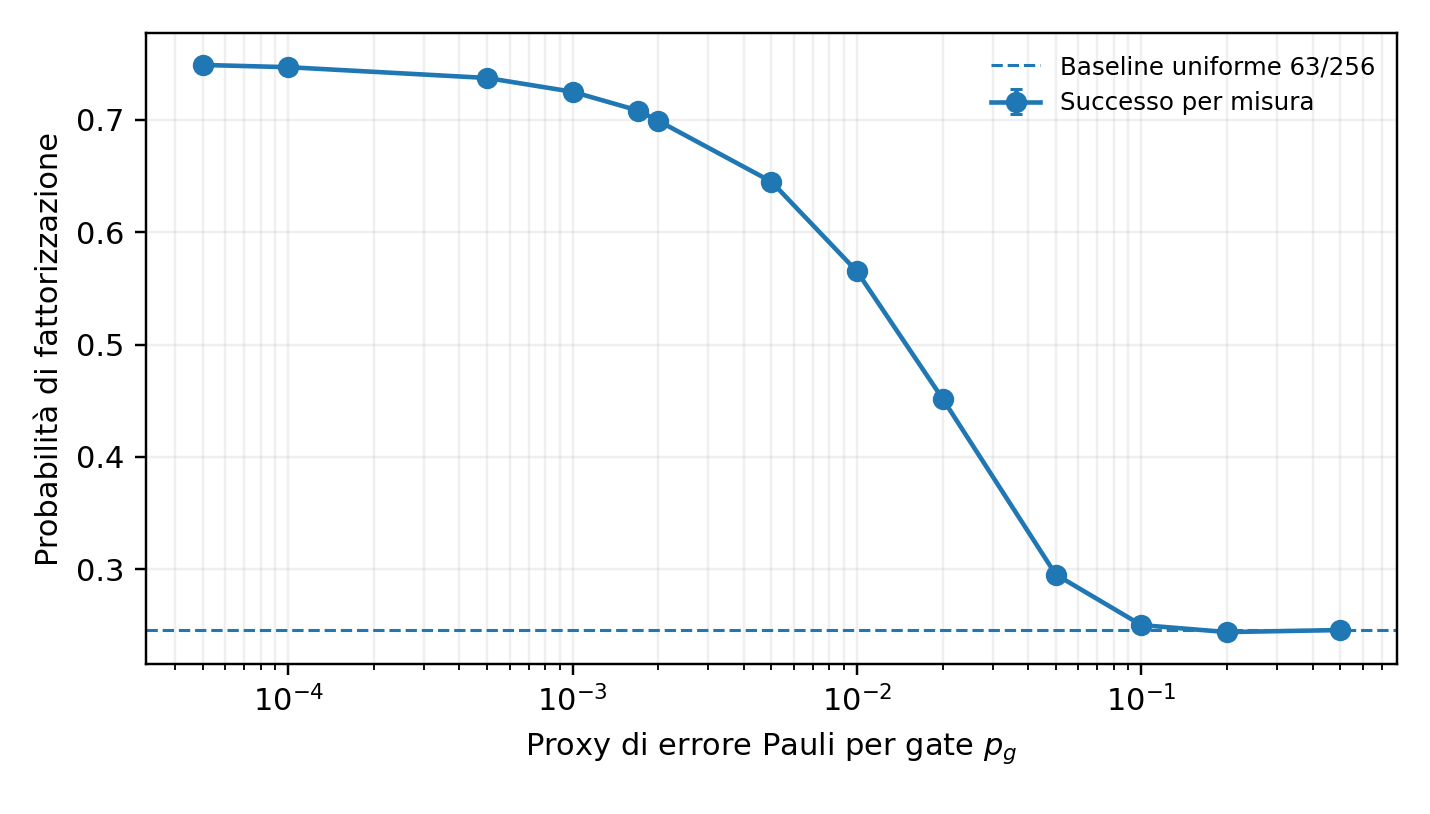
\includegraphics[width=0.85\textwidth,height=0.68\textheight,keepaspectratio]{finale_fig_5_7_shor_successo_proxy_gate.png}

\caption{Probabilità di fattorizzazione in funzione del proxy per gate p\_g. La linea orizzontale indica la baseline uniforme 63/256.}\label{fig:finale_5_7}
\end{figure}

\subsection{Il plateau vicino a 63/256 e il significato del successo residuo}\label{sec:finale_5_4_2}

Per p\_g≥0.1 il successo si stabilizza intorno a 0.245, praticamente coincidente con 63/256=0.2461. Questo comportamento è coerente con la perdita della struttura quantistica utile e con il fatto che la procedura classica accetta comunque 63 dei 256 possibili valori. Il plateau non è quindi una soglia universale di Shor, né prova la presenza di informazione quantistica residua: è una proprietà congiunta dell'istanza N=15, del registro a otto bit e della funzione di estrazione dei fattori.

Questa distinzione è cruciale per interpretare correttamente le metriche. Una percentuale di fattorizzazioni corrette può rimanere non nulla anche quando la distribuzione si avvicina a un fondo quasi uniforme. Per questo, nella tesi il successo per misura viene letto insieme alla struttura dell'istogramma e alle baseline combinatorie, non come proxy di fedeltà dello stato.

\subsection{Ripetizioni indipendenti e robustezza di TOP-4}\label{sec:finale_5_4_3}

Per tentativi indipendenti, la probabilità cumulativa di ottenere almeno un successo dopo k esecuzioni è P(k)=1-(1-P\_s)\^{}k. Il numero di tentativi richiesto cresce rapidamente quando il successo per singola misura degrada. Con P\_s=0.7489, due tentativi portano a circa 0.937; con p\_g=0.01, due tentativi danno circa 0.811; con p\_g=0.05 servono cinque tentativi per superare l'80\%, e con p\_g=0.2 ne servono sei.

\begin{figure}[H]
\centering
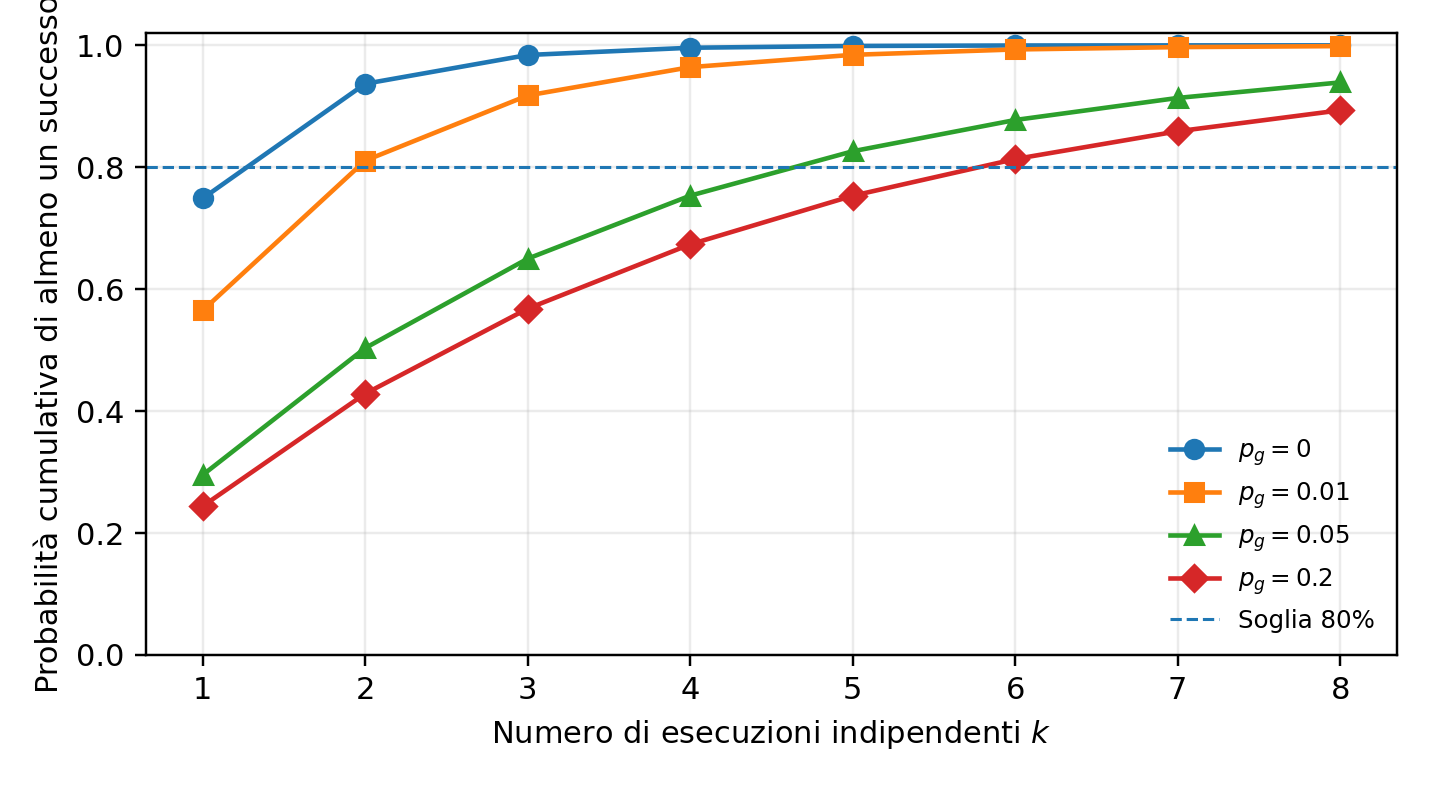
\includegraphics[width=0.85\textwidth,height=0.68\textheight,keepaspectratio]{finale_fig_5_8_shor_probabilita_cumulativa.png}

\caption{Probabilità cumulativa di almeno una fattorizzazione riuscita dopo k esecuzioni indipendenti.}\label{fig:finale_5_8}\label{fig:qec_shor_pk}
\end{figure}

M13 verifica separatamente TOP-4 lungo lo stesso asse di rumore, usando 200 repliche da 1 024 shot. TOP-4 rimane pari a 1.000 fino a p\_g=0.05, benché la massa utile per singola misura scenda da circa 0.7512 a 0.2979. A p\_g=0.2 il successo TOP-4 scende a 0.670; l'intervallo identificato {[}0.535;0.860{]} riflette la gestione dei pareggi al confine del quarto candidato. Il contrasto predefinito nel protocollo rispetto a p\_g=0 mostra una diminuzione di 0.330 con IC Newcombe 95\% {[}0.266;0.398{]}. Il risultato conferma che TOP-4 è operativo anche quando la distribuzione è degradata, ma proprio per questo non può essere usato come misura di fedeltà del circuito.

\begingroup
\small
\begin{table}[!htbp]
\centering
\small

\begin{tabular}{@{}
  >{\raggedright\arraybackslash}p{(\linewidth - 8\tabcolsep) * \real{0.1613}}
  >{\centering\arraybackslash}p{(\linewidth - 8\tabcolsep) * \real{0.2204}}
  >{\centering\arraybackslash}p{(\linewidth - 8\tabcolsep) * \real{0.1290}}
  >{\centering\arraybackslash}p{(\linewidth - 8\tabcolsep) * \real{0.1683}}
  >{\centering\arraybackslash}p{(\linewidth - 8\tabcolsep) * \real{0.3209}}@{}}
\toprule
\textbf{$p_g$} & \textbf{Successo per misura} & \textbf{TOP-1} & \textbf{TOP-4 seeded} & \textbf{Intervallo identificato TOP-4} \\
\midrule
0 & 0.7512 & 0.805 & 1.000 & {[}1.000;1.000{]} \\
\addlinespace[0.3em]
10⁻⁴ & 0.7459 & 0.730 & 1.000 & {[}1.000;1.000{]} \\
\addlinespace[0.3em]
5×10⁻⁴ & 0.7377 & 0.690 & 1.000 & {[}1.000;1.000{]} \\
\addlinespace[0.3em]
10⁻³ & 0.7229 & 0.620 & 1.000 & {[}1.000;1.000{]} \\
\addlinespace[0.3em]
1.7×10⁻³ & 0.7080 & 0.620 & 1.000 & {[}1.000;1.000{]} \\
\addlinespace[0.3em]
2×10⁻³ & 0.7003 & 0.650 & 1.000 & {[}1.000;1.000{]} \\
\addlinespace[0.3em]
5×10⁻³ & 0.6396 & 0.505 & 1.000 & {[}1.000;1.000{]} \\
\addlinespace[0.3em]
10⁻² & 0.5652 & 0.645 & 1.000 & {[}1.000;1.000{]} \\
\addlinespace[0.3em]
2×10⁻² & 0.4528 & 0.695 & 1.000 & {[}1.000;1.000{]} \\
\addlinespace[0.3em]
5×10⁻² & 0.2979 & 0.760 & 1.000 & {[}1.000;1.000{]} \\
\addlinespace[0.3em]
10⁻¹ & 0.2506 & 0.535 & 0.915 & {[}0.855;0.940{]} \\
\addlinespace[0.3em]
2×10⁻¹ & 0.2469 & 0.245 & 0.670 & {[}0.535;0.860{]} \\
\bottomrule
\end{tabular}
\caption{M13: TOP-4 sotto il proxy $p_g$. Il successo TOP-K deve essere letto insieme alla massa utile per misura e all'incertezza dei pareggi.}\label{tab:finale_5_20}

\end{table}
\endgroup

\subsection{Controlli hardware-aware: layout e readout}\label{sec:finale_5_4_4}

Due analisi esplorative usano una snapshot offline di FakeSherbrooke per verificare se parametri hardware-aware possano ordinare il successo simulato. In M11, 40 dei 60 layout richiesti rientrano nel dominio del modello. La correlazione di Spearman fra un punteggio aggregato di calibrazione e il successo holdout è ρ\_s=-0.184, con IC bootstrap 95\% {[}-0.456;0.124{]}: il campione non supporta una capacità predittiva conclusiva del punteggio aggregato. La regola che sceglie il layout con punteggio minimo ottiene P\_holdout=0.451; quella che sceglie il massimo successo sui dati di selezione ottiene 0.516, differenza descrittiva di 0.065 senza intervallo dedicato. Questi controlli restano osservazionali e non sostituiscono una validazione hardware. La scelta di valutare layout e readout come variabili di controllo è coerente con la letteratura sulla compilazione noise-adaptive e sulle politiche di mapping sensibili all'eterogeneità dei qubit \cite{murali2019,tannu2019}.

M11b analizza nove sottografi e misura il readout dei qubit effettivamente misurati dopo il routing. Condizionando per sottografo, numero di ECR e profondità, la correlazione parziale con il successo è ρ\_s=-0.605 con IC cluster bootstrap 95\% {[}-0.826;-0.190{]}. Un readout peggiore si associa quindi a un successo inferiore nel campione, ma nove cluster non consentono di trasformare questa associazione in una relazione causale né di validare una strategia generale di placement.

\begingroup
\small
\begin{table}[!htbp]
\centering
\small

\begin{tabular}{@{}
  >{\raggedright\arraybackslash}p{(\linewidth - 6\tabcolsep) * \real{0.2857}}
  >{\raggedright\arraybackslash}p{(\linewidth - 6\tabcolsep) * \real{0.2338}}
  >{\raggedright\arraybackslash}p{(\linewidth - 6\tabcolsep) * \real{0.2338}}
  >{\raggedright\arraybackslash}p{(\linewidth - 6\tabcolsep) * \real{0.2468}}@{}}
\toprule
\textbf{Controllo} & \textbf{Campione} & \textbf{Stima principale} & \textbf{Interpretazione ammessa} \\
\midrule
M11: score aggregato & 40 layout validi & $\rho_s$=-0.184; IC {[}-0.456;0.124{]} & nessuna capacità predittiva conclusiva \\
\addlinespace[0.3em]
M11b: readout post-routing & 9 sottografi, 45 osservazioni & $\rho_s$ parziale=-0.605; IC {[}-0.826;-0.190{]} & associazione osservata, non prova causale \\
\bottomrule
\end{tabular}
\caption{Controlli hardware-aware su snapshot offline FakeSherbrooke.}\label{tab:finale_5_21}

\end{table}
\endgroup

\par\medskip\noindent\rule{\linewidth}{0.6pt}\par\nopagebreak
{\small\setstretch{1.15}\noindent \textbf{Risposta a DR4.} Nel modello M8, la probabilità di fattorizzazione diminuisce al crescere del proxy per gate p\_g e converge verso la baseline uniforme specifica della procedura di estrazione. Le ripetizioni indipendenti compensano probabilisticamente un singolo run meno affidabile, ma non eliminano il costo del rumore. Le metriche QEC non vengono proiettate su questa curva: trasformare p\_L di una memoria in p\_g di una computazione richiederebbe una compilazione fault-tolerant esplicita.\par}
\nopagebreak\noindent\rule{\linewidth}{0.6pt}\par\medskip

\section{DR5 - QFT approssimata: quando meno porte producono più informazione utile}\label{sec:finale_5_5}\label{sec:qft_topologia}

La quinta domanda di ricerca studia un compromesso diverso: eliminare rotazioni controllate di piccolo angolo riduce il numero di porte e la profondità, ma introduce un errore algoritmico. Il beneficio esiste soltanto se il rumore evitato compensa l'informazione di fase persa. Per evitare una conclusione unica su circuiti molto differenti, la campagna distingue tre casi: Shor su N=15, Shor con aritmetica Beauregard su N=21 e Quantum Phase Estimation isolata. L'idea di eliminare rotazioni di piccolo angolo ha una tradizione teorica consolidata nell'AQFT; il punto qui è verificarne il beneficio sulla metrica algoritmica effettiva \cite{barencoAQFT1996,akoramurthy2026}.

\subsection{Shor su N=15: miglioramento misurato su holdout}\label{sec:finale_5_5_1}

Per N=15, a=7, il grado di troncamento k\_QPE viene scelto sui batch di selezione e valutato su holdout disgiunti. Ogni configurazione usa 8 192 shot, divisi in otto batch. La selezione sceglie k\_QPE=1. Sull'holdout, la probabilità di successo sale da 0.4792 con la QFT piena a 0.6279 con la variante troncata: +0.1487, con IC Newcombe 95\% {[}0.1273;0.1699{]}. Contemporaneamente, le porte ECR scendono da 362 a 279 e la profondità da 1 351 a 1 141.

\begingroup
\small
\begin{table}[!htbp]
\centering
\small

\begin{tabular}{@{}
  >{\raggedright\arraybackslash}p{(\linewidth - 6\tabcolsep) * \real{0.2200}}
  >{\centering\arraybackslash}p{(\linewidth - 6\tabcolsep) * \real{0.1000}}
  >{\centering\arraybackslash}p{(\linewidth - 6\tabcolsep) * \real{0.2800}}
  >{\centering\arraybackslash}p{(\linewidth - 6\tabcolsep) * \real{0.4000}}@{}}
\toprule
\textbf{$k_{\mathrm{QPE}}$} & \textbf{ECR} & \textbf{Profondità} & \textbf{$P_{\mathrm{success}}$ holdout} \\
\midrule
1 & 279 & 1 141 & 0.6279 \\
\addlinespace[0.3em]
2 & 305 & 1 242 & 0.5422 \\
\addlinespace[0.3em]
3 & 328 & 1 330 & 0.5210 \\
\addlinespace[0.3em]
4 & 360 & 1 414 & 0.4771 \\
\addlinespace[0.3em]
5 & 365 & 1 391 & 0.4607 \\
\addlinespace[0.3em]
6 & 360 & 1 306 & 0.4749 \\
\addlinespace[0.3em]
7 (piena) & 362 & 1 351 & 0.4792 \\
\bottomrule
\end{tabular}
\caption{Griglia AQFT su Shor N=15. La configurazione $k_{\mathrm{QPE}}=1$ è scelta sui dati di selezione e valutata sull'holdout.}\label{tab:finale_5_22}

\end{table}
\endgroup

\begin{figure}[H]
\centering
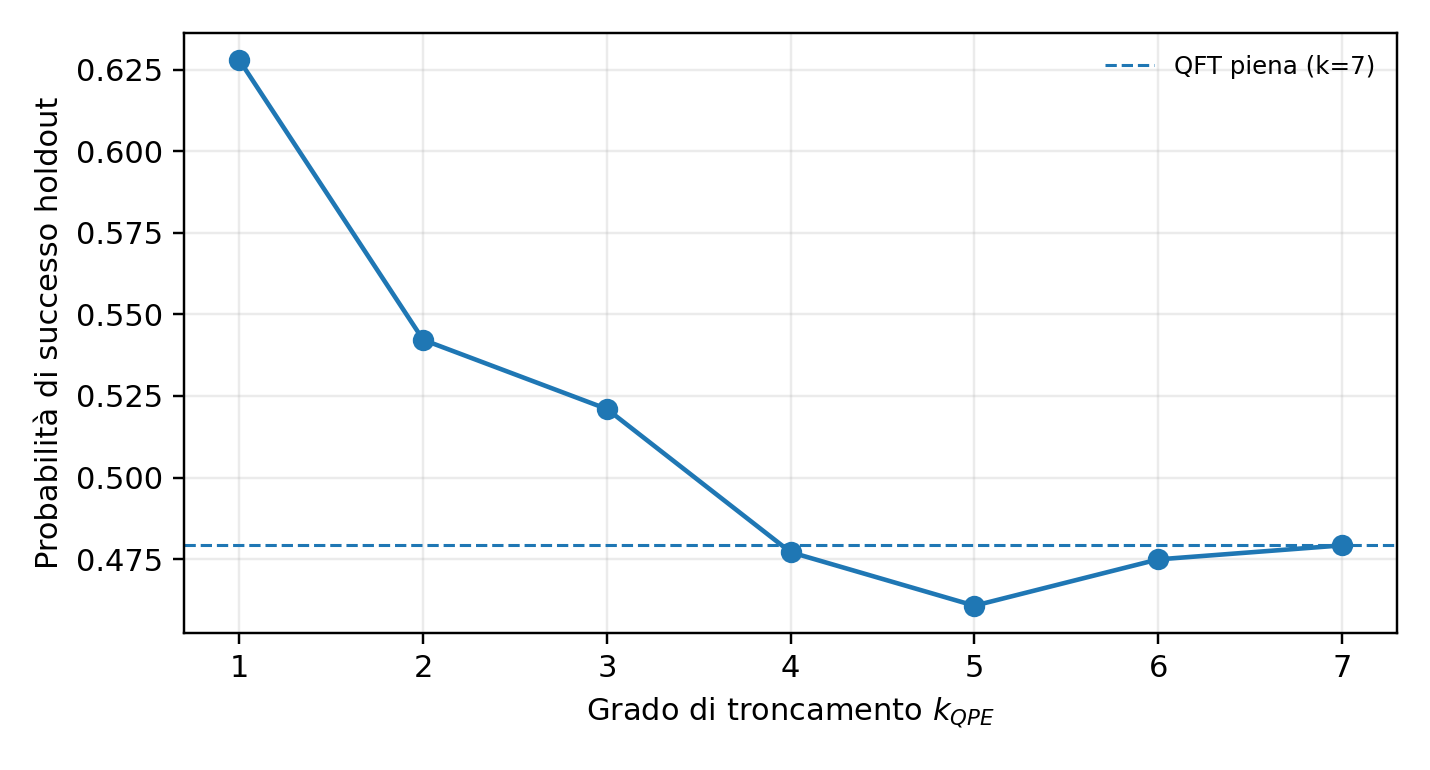
\includegraphics[width=0.85\textwidth,height=0.68\textheight,keepaspectratio]{finale_fig_5_9_aqft_n15_holdout.png}

\caption{Successo holdout al variare del grado di troncamento della QFT inversa finale per N=15.}\label{fig:finale_5_9}
\end{figure}

Il miglioramento è rilevante sia in termini assoluti sia ingegneristici: +14.87 punti percentuali di successo, circa +31\% in termini relativi; -83 porte ECR, circa -22.9\%; profondità ridotta di circa 15.5\%. Nel perimetro dell'istanza N=15, il risultato è positivo anche sulla metrica finale di fattorizzazione, non soltanto su una subroutine isolata.

\begingroup
\small
\begin{table}[!htbp]
\centering
\small

\begin{tabular}{@{}
  >{\raggedright\arraybackslash}p{(\linewidth - 6\tabcolsep) * \real{0.2812}}
  >{\centering\arraybackslash}p{(\linewidth - 6\tabcolsep) * \real{0.1656}}
  >{\centering\arraybackslash}p{(\linewidth - 6\tabcolsep) * \real{0.2016}}
  >{\centering\arraybackslash}p{(\linewidth - 6\tabcolsep) * \real{0.3516}}@{}}
\toprule
\textbf{Indicatore} & \textbf{QFT piena} & \textbf{AQFT scelta} & \textbf{Variazione} \\
\midrule
$P_{\mathrm{success}}$ holdout & 0.4792 & 0.6279 & +14.87 punti percentuali \\
\addlinespace[0.3em]
Porte ECR & 362 & 279 & -83 (-22.9\%) \\
\addlinespace[0.3em]
Profondità & 1 351 & 1 141 & -210 (-15.5\%) \\
\bottomrule
\end{tabular}
\caption{Sintesi del beneficio AQFT misurato su N=15.}\label{tab:finale_5_23}

\end{table}
\endgroup

La generalizzazione deve però essere limitata. L'ordine r=4 genera fasi 0, 1/4, 1/2 e 3/4, rappresentabili esattamente con due bit. Le rotazioni più fini sono quindi meno informative in questa specifica istanza e la riduzione di rumore può dominare la perdita di precisione. La stessa condizione non vale automaticamente per ordini diversi.

\subsection{Shor su N=21: grande riduzione di porte, beneficio non dimostrato}\label{sec:finale_5_5_2}

Nel circuito Beauregard per N=21 la maggior parte del costo non è nella QFT finale della QPE, ma nelle trasformate interne agli addizionatori modulari. Nella compilazione utilizzata per la sensibilità rumorosa, il troncamento porta le ECR da 49 661 a 23 178, una riduzione di circa il 53.3\%. Il prezzo algoritmico è però visibile già senza rumore: il successo ideale scende da 0.4667 a 0.4013, cioè di 6.54 punti percentuali.

\begingroup
\small
\begin{table}[!htbp]
\centering
\small

\begin{tabular}{@{}
  >{\raggedright\arraybackslash}p{(\linewidth - 6\tabcolsep) * \real{0.2752}}
  >{\centering\arraybackslash}p{(\linewidth - 6\tabcolsep) * \real{0.2212}}
  >{\centering\arraybackslash}p{(\linewidth - 6\tabcolsep) * \real{0.2386}}
  >{\centering\arraybackslash}p{(\linewidth - 6\tabcolsep) * \real{0.2650}}@{}}
\toprule
\textbf{Voce} & \textbf{Versione piena} & \textbf{Versione troncata} & \textbf{Variazione} \\
\midrule
ECR nella compilazione rumorosa & 49 661 & 23 178 & -53.3\% \\
\addlinespace[0.3em]
Successo ideale & 0.4667 & 0.4013 & -0.0654 \\
\addlinespace[0.3em]
QFT finale QPE & 28 rotazioni & non dominante & costo marginale rispetto all'aritmetica \\
\bottomrule
\end{tabular}
\caption{Bilancio strutturale dell'AQFT su N=21.}\label{tab:finale_5_24}

\end{table}
\endgroup

\begingroup
\small
\begin{table}[!htbp]
\centering
\small

\begin{tabular}{@{}
  >{\raggedright\arraybackslash}p{(\linewidth - 8\tabcolsep) * \real{0.1389}}
  >{\centering\arraybackslash}p{(\linewidth - 8\tabcolsep) * \real{0.1944}}
  >{\centering\arraybackslash}p{(\linewidth - 8\tabcolsep) * \real{0.1944}}
  >{\centering\arraybackslash}p{(\linewidth - 8\tabcolsep) * \real{0.1944}}
  >{\centering\arraybackslash}p{(\linewidth - 8\tabcolsep) * \real{0.2778}}@{}}
\toprule
\textbf{Fattore di rumore} & \textbf{QFT/\allowbreak{}arithmetic full} & \textbf{Aritmetica troncata} & \textbf{Differenza} & \textbf{IC 95\%} \\
\midrule
0.03 & 0.2813 & 0.2891 & +0.0078 & {[}-0.1020; +0.1174{]} \\
\addlinespace[0.3em]
0.01 & 0.2734 & 0.2734 & 0.0000 & {[}-0.1084; +0.1084{]} \\
\addlinespace[0.3em]
0.003 & 0.3828 & 0.2734 & -0.1094 & {[}-0.2205; +0.0056{]} \\
\bottomrule
\end{tabular}
\caption{Test rumorosi esplorativi su N=21. Tutti gli intervalli includono lo zero.}\label{tab:finale_5_25}

\end{table}
\endgroup

Nelle prove rumorose a budget ridotto nessun confronto dimostra un vantaggio della variante troncata: gli intervalli includono sempre lo zero e, al fattore 0.003, la QFT piena è quella con successo maggiore. Un modello ausiliario a miscela stima che, in condizioni di porte molto migliori, il risparmio di operazioni potrebbe generare un margine dell'ordine di tre punti percentuali; la stessa stima richiede errori 2Q circa duecento volte inferiori a quelli della calibrazione considerata. È quindi un'ipotesi di progetto, non un risultato misurato.

\subsection{Quantum Phase Estimation isolata: evidenza favorevole ma esplorativa}\label{sec:finale_5_5_3}

Per separare l'effetto dell'AQFT dal costo dell'aritmetica modulare, la campagna ripete il confronto sulla sola stima di fase. Vengono considerate tre dimensioni del registro, n=6,8,10, e tre fasi per dimensione. Il grado di troncamento viene scelto sui batch di selezione; la differenza viene misurata su holdout usando lo stesso layout e la stessa sequenza dei seed per i due bracci.

\begingroup
\small
\begin{table}[!htbp]
\centering
\small

\begin{tabular}{@{}
  >{\raggedright\arraybackslash}p{(\linewidth - 12\tabcolsep) * \real{0.0735}}
  >{\centering\arraybackslash}p{(\linewidth - 12\tabcolsep) * \real{0.1324}}
  >{\centering\arraybackslash}p{(\linewidth - 12\tabcolsep) * \real{0.1324}}
  >{\centering\arraybackslash}p{(\linewidth - 12\tabcolsep) * \real{0.1176}}
  >{\centering\arraybackslash}p{(\linewidth - 12\tabcolsep) * \real{0.1176}}
  >{\centering\arraybackslash}p{(\linewidth - 12\tabcolsep) * \real{0.1324}}
  >{\centering\arraybackslash}p{(\linewidth - 12\tabcolsep) * \real{0.2941}}@{}}
\toprule
\textbf{n} & \textbf{Fase} & \textbf{k scelto} & \textbf{AQFT} & \textbf{QFT piena} & \textbf{Δ} & \textbf{IC 95\%} \\
\midrule
6 & 1/6 & 2 & 0.3755 & 0.3599 & +0.0156 & {[}-0.0139; +0.0451{]} \\
\addlinespace[0.3em]
6 & 21/2⁶ & 2 & 0.5576 & 0.5059 & +0.0518 & {[}+0.0212; +0.0822{]} \\
\addlinespace[0.3em]
6 & 1/3 & 2 & 0.3564 & 0.3418 & +0.0146 & {[}-0.0145; +0.0438{]} \\
\addlinespace[0.7em]
8 & 1/6 & 3 & 0.2861 & 0.2598 & +0.0264 & {[}-0.0009; +0.0536{]} \\
\addlinespace[0.3em]
8 & 85/2⁸ & 3 & 0.4014 & 0.3545 & +0.0469 & {[}+0.0172; +0.0765{]} \\
\addlinespace[0.3em]
8 & 1/3 & 3 & 0.2930 & 0.2500 & +0.0430 & {[}+0.0157; +0.0701{]} \\
\addlinespace[0.7em]
10 & 1/6 & 2 & 0.2354 & 0.1641 & +0.0713 & {[}+0.0469; +0.0956{]} \\
\addlinespace[0.3em]
10 & 341/2¹⁰ & 2 & 0.3564 & 0.2310 & +0.1255 & {[}+0.0977; +0.1530{]} \\
\addlinespace[0.3em]
10 & 1/3 & 2 & 0.2280 & 0.1733 & +0.0547 & {[}+0.0302; +0.0791{]} \\
\bottomrule
\end{tabular}
\caption{Benchmark QPE: differenza holdout fra variante selezionata e QFT piena. Gli intervalli sono individuali; la campagna non applica una correzione simultanea ai nove confronti.}\label{tab:finale_5_26}

\end{table}
\endgroup

\begin{figure}[H]
\centering
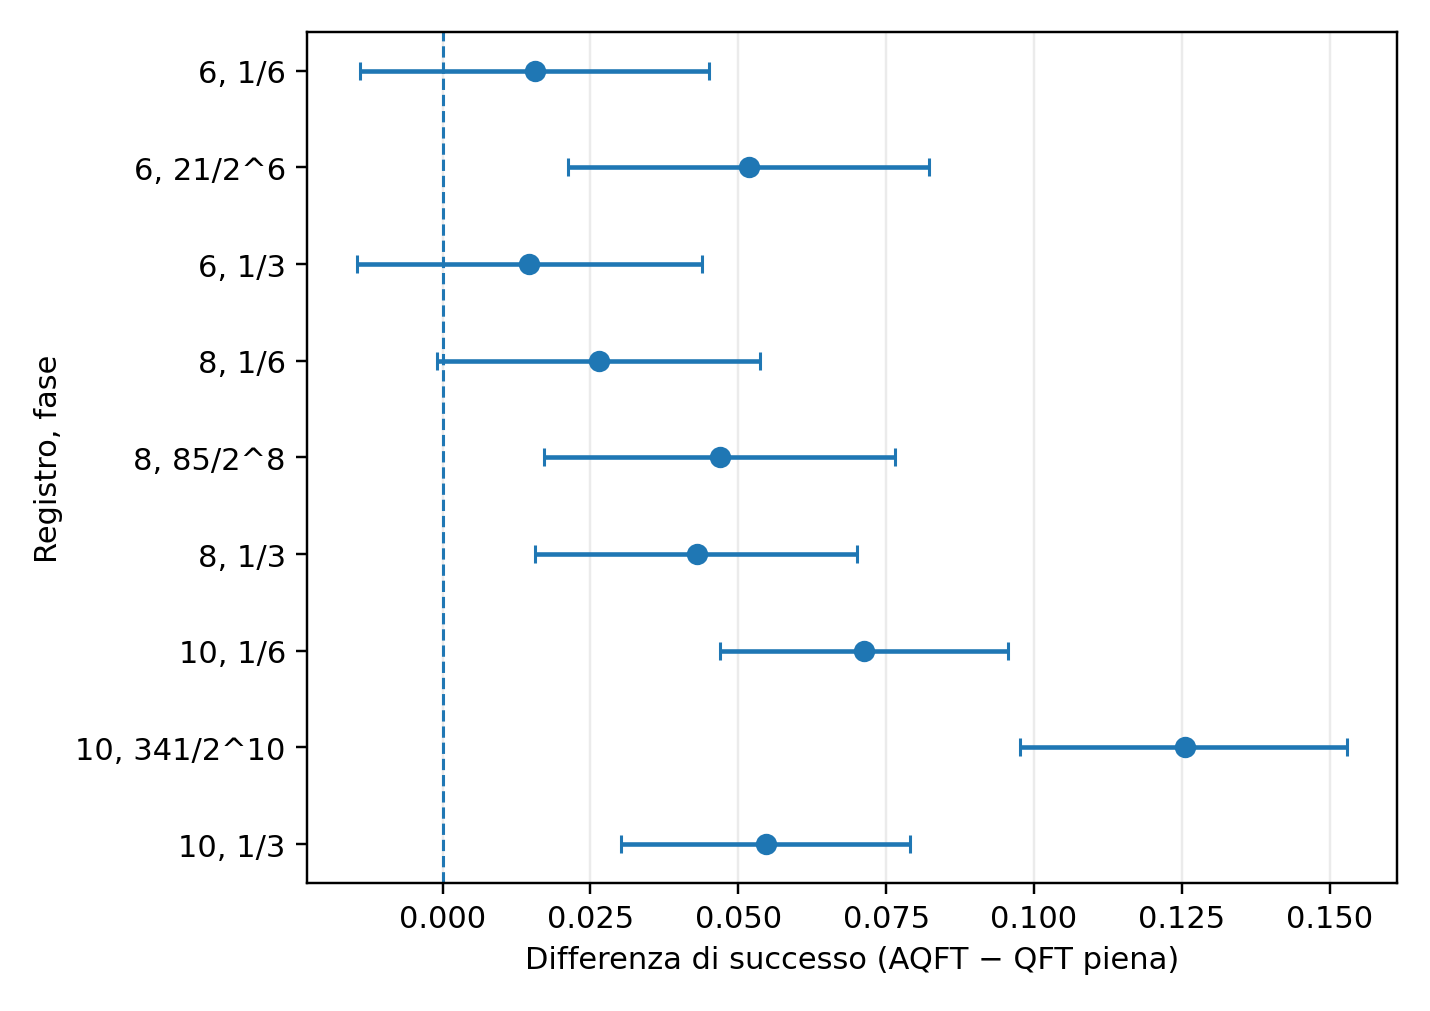
\includegraphics[width=0.85\textwidth,height=0.68\textheight,keepaspectratio]{finale_fig_5_10_aqft_qpe_holdout.png}

\caption{Differenze di successo AQFT-QFT piena nei nove benchmark QPE, con IC Newcombe individuali al 95\%.}\label{fig:finale_5_10}
\end{figure}

Le stime sono positive in tutti e nove i confronti e sei intervalli individuali escludono lo zero. Il massimo incremento è +0.1255 su dieci qubit, con IC {[}0.0977;0.1530{]}. Il grado più favorevole fra quelli provati è 2 o 3, mentre la QFT piena utilizza n-1 livelli di rotazione; i risparmi di ECR crescono da 25 a n=6 a 78 a n=10. La tendenza è quindi coerente con l'idea che, in circuiti relativamente corti, eliminare rotazioni fini possa ridurre più rumore di quanto perda informazione.

\subsection{Interpretazione: il grado ottimo dipende dall'informazione di fase}\label{sec:finale_5_5_4}

I tre esperimenti convergono su un criterio più utile di una semplice etichetta ``AQFT sì/no''. Per N=15 il periodo r=4 produce fasi esattamente rappresentabili con pochi bit e il troncamento è favorevole. Per N=21, r=6 produce fasi j/6, non tutte rappresentabili esattamente nel registro finito: le rotazioni più fini conservano quindi informazione utile e la perdita algoritmica può superare il vantaggio circuitale. Nel benchmark QPE le fasi esattamente rappresentabili sono, in generale, quelle che beneficiano maggiormente del troncamento.

Il limite teorico discusso in letteratura \cite{barencoAQFT1996,akoramurthy2026} fornisce inoltre una cautela alla scala: la distanza in variazione totale fra QPE esatta e troncata può essere limitata da un termine proporzionale a π(m-d)/2\^{}d. Per mantenere controllato tale errore, il grado di troncamento deve crescere circa logaritmicamente con la dimensione del registro. Il fatto che k=2 o 3 sia favorevole nelle taglie provate non autorizza quindi a considerare costante il grado ottimo per registri arbitrariamente grandi.

\par\medskip\noindent\rule{\linewidth}{0.6pt}\par\nopagebreak
{\small\setstretch{1.15}\noindent \textbf{Risposta a DR5.} L'AQFT è efficace quando il risparmio di porte supera la perdita di precisione di fase. Questo avviene in modo netto su Shor N=15 e in diversi benchmark di QPE; non è invece dimostrato nelle prove rumorose su N=21, dove l'aritmetica è molto più profonda e le fasi richiedono maggiore precisione. Il risultato scientifico è quindi un criterio di progetto dipendente da istanza, fase e regime di rumore, non una sostituzione universale della QFT completa.\par}
\nopagebreak\noindent\rule{\linewidth}{0.6pt}\par\medskip

\section{Discussione integrata dei risultati}\label{sec:finale_5_6}

Le cinque domande di ricerca descrivono interventi collocati in punti diversi della catena computazionale. La loro lettura congiunta permette di separare tre concetti che, se osservati isolatamente, possono essere facilmente confusi: utilizzare meglio l'informazione residua, proteggere l'informazione durante l'evoluzione e ridurre il costo fisico necessario a produrla. Le metriche non sono convertibili fra loro, ma il principio sperimentale che le governa è comune.

\subsection{Una gerarchia delle evidenze}\label{sec:finale_5_6_1}

Il primo risultato è metodologico. Una metrica intermedia elevata non basta a dimostrare un vantaggio sul compito finale. La SVM della fase NISQ raggiunge AUC superiore a 0.95, ma TOP-4 senza classificatore richiede meno iterazioni. Analogamente, un TOP-K vicino al 100\% non implica uno stato quantistico fedele, perché la verifica classica dell'istanza N=15 accetta 63 risultati su 256. L'ablazione e la baseline combinatoria impediscono quindi due conclusioni apparentemente plausibili ma scorrette.

Il secondo risultato riguarda la QEC. Qui il beneficio non è post-processing: sotto soglia la codifica modifica effettivamente l'ordine dell'errore. Il repetition code e Steane mostrano soppressione quadratica nel rispettivo modello; il surface code aggiunge la dipendenza dalla distanza e un comportamento di soglia. Il costo è l'overhead fisico, e le estrapolazioni mostrano quanto la qualità dei qubit influenzi direttamente il numero di risorse necessarie a proteggere una memoria.

Il terzo risultato riguarda l'apprendimento nella decodifica. La rete non è superiore per definizione. Quando il decoder analitico dispone di un modello rappresentabile e viene scelto bene, l'analitico rimane competitivo o migliore. Quando compaiono correlazioni che la struttura del decoder non sa rappresentare, il modello appreso può recuperare una parte del margine. Questa conclusione è più informativa di una semplice dicotomia ``ML funziona/non funziona'', perché identifica la condizione informativa che rende utile la complessità aggiuntiva.

Il quarto risultato riguarda l'ottimizzazione del circuito. L'AQFT dimostra che una trasformazione algoritmicamente approssimata può produrre un risultato finale migliore quando elimina abbastanza operazioni rumorose. Ma il vantaggio dipende dalla struttura di fase: su N=15 è misurato e statisticamente netto; su N=21 non emerge; nella QPE isolata ricompare in modo consistente. La profondità del circuito non è quindi un semplice costo accessorio: può modificare quale approssimazione sia ottimale per il compito.

\subsection{Il criterio unificante: la complessità deve agire sul collo di bottiglia reale}\label{sec:finale_5_6_2}

I risultati suggeriscono un criterio comune. Una componente aggiuntiva è giustificata quando utilizza informazione che la baseline non sfrutta oppure quando elimina un costo fisico superiore alla perdita algoritmica introdotta. TOP-4 soddisfa il primo criterio perché prova candidati già presenti nell'istogramma; il classificatore a valle no, perché non aggiunge informazione utile rispetto alla stessa ricerca. Il decoder ibrido soddisfa il criterio soltanto quando la sindrome contiene correlazioni non rappresentate dal decoder analitico. BP+OSD mostra invece che, quando il modello è rappresentabile, migliorare prima la baseline analitica può essere la scelta più efficiente. L'AQFT soddisfa il secondo criterio quando la riduzione delle porte compensa l'errore di troncamento.

Anche i risultati negativi sono informativi. Il mancato vantaggio del filtro ML, l'assenza di guadagno AQFT su N=21 e la non additività fra BP+OSD e residuo delimitano il dominio di validità delle tecniche e riducono il rischio di attribuire il miglioramento alla causa sbagliata. In una tesi sperimentale, stabilire dove una tecnica non produce un beneficio misurabile è parte dell'evidenza, purché baseline, metriche e protocollo siano definiti prima dell'interpretazione.

\subsection{Cosa i risultati dimostrano e cosa rimane aperto}\label{sec:finale_5_6_3}

Nel perimetro simulativo adottato, i risultati mostrano che la ricerca multi-candidato può ridurre il costo operativo su N=15; che codici di distanza crescente mostrano soppressione e comportamento di soglia nei memory experiment; che un correttore residuale appreso può ridurre l'errore quando la struttura del decoder è incompleta; che il successo della specifica implementazione di Shor degrada fino al pavimento uniforme al crescere del proxy per gate; e che una QFT troncata può aumentare il successo quando il risparmio circuitale domina la perdita di precisione.

Non viene invece dimostrata un'esecuzione end-to-end fault-tolerant di Shor. I tassi p\_L dei memory experiment non sono errori di porte logiche e non vengono convertiti in p\_g. Le campagne principali non sono eseguite su hardware reale; FakeSherbrooke è una snapshot offline e i modelli uniformi non riproducono deriva, leakage, crosstalk e routing nello stesso esperimento. L'istanza rumorosa principale è N=15, che ha caratteristiche particolarmente favorevoli sia al TOP-K sia all'AQFT. Le estensioni a moduli maggiori devono quindi variare separatamente dimensione di N, ordine r, topologia, calibrazione e aritmetica.

Questi limiti non riducono il valore del lavoro; ne definiscono correttamente il livello di evidenza. Il contributo non è una previsione di quando Shor diventerà crittograficamente praticabile, ma un insieme di verifiche controllate che mostrano come distinguere beneficio reale, beneficio apparente e costo nascosto quando rumore, post-processing, correzione d'errore, decoder e approssimazione circuitale interagiscono.

\subsection{Sintesi del capitolo}\label{sec:finale_5_6_4}


Il Capitolo 6 riprende questi risultati per rispondere in forma conclusiva alle domande di ricerca, distinguendo contributi, limiti e sviluppi futuri. La conclusione generale non è che una singola tecnica risolva il problema del rumore, ma che l'efficacia di ogni intervento dipende dalla posizione in cui agisce e dall'informazione o dal costo che riesce realmente a modificare.

\chapter{Conclusioni e sviluppi futuri}
\label{chap:conclusioni}
\label{chap:sviluppi}

% Generato dalla versione Word revisionata e dalla bozza auditata.
% Le citazioni numeriche originali sono state convertite in chiavi BibLaTeX.

% Conclusioni compatte: le evidenze numeriche complete restano nel Capitolo 5
% e nelle appendici sperimentali.

Questo capitolo risponde alle cinque domande di ricerca senza duplicare le tabelle del Capitolo~\ref{chap:risultati}. I risultati sono interpretati entro il perimetro dichiarato nei Capitoli 3 e 4: simulazioni controllate, istanze di piccola scala e separazione esplicita fra errore fisico, errore logico e proxy applicato al circuito di Shor.

\section{Risposte alle domande di ricerca}\label{sec:finale_6_1}

La Tabella~\ref{tab:finale_6_1} riporta per ogni domanda risposta, evidenza e limite. Numerosità, intervalli e controlli completi rimangono nelle rispettive sezioni del Capitolo~\ref{chap:risultati}.

\begingroup
\footnotesize
\begin{spacing}{1.0}
\begin{table}[!htbp]
\centering
\small

\begin{tabular}{@{}
  >{\raggedright\arraybackslash}p{(\linewidth - 6\tabcolsep) * \real{0.08}}
  >{\raggedright\arraybackslash}p{(\linewidth - 6\tabcolsep) * \real{0.32}}
  >{\raggedright\arraybackslash}p{(\linewidth - 6\tabcolsep) * \real{0.3}}
  >{\raggedright\arraybackslash}p{(\linewidth - 6\tabcolsep) * \real{0.3}}@{}}
\toprule
\textbf{DR} & \textbf{Risposta} & \textbf{Evidenza} & \textbf{Limite} \\
\midrule
DR1 & TOP-$K$ è utile; il filtro ML considerato non aggiunge valore operativo. & TOP-4 raggiunge 1.00 iterazioni medie nei due scenari; M2 perde contro la propria ablazione. & $N=15$ e post-processing specifico. \\
\addlinespace[0.3em]
DR2 & La QEC sopprime l'errore sotto soglia e il beneficio cresce con la distanza. & Steane: pendenza 1.94; surface code: $p_{th}\simeq0.86\%$ (Z) e $0.81\%$ (X). & Memory experiment, non Shor fault-tolerant. \\
\addlinespace[0.3em]
DR3 & Il ML è utile come correttore residuale quando il decoder è strutturalmente incompleto; il decoder conta anche nel confronto fra codici. & A $d=3$ la riduzione relativa è 15.6--17.6\% con crosstalk; BP+OSD resta una baseline forte; il Gross code batte 12 patch a $d=13$ per $p\ge0.75\%$. & MLP denso; nessun vantaggio significativo a $d=7$; Gross code solo in code-capacity. \\
\addlinespace[0.3em]
DR4 & Il successo di Shor decresce con $p_g$ e tende al pavimento del post-processing. & Da 0.7489 a $p_g=0$ a circa 0.245 per rumore elevato. & Proxy fenomenologico, non tasso logico QEC. \\
\addlinespace[0.3em]
DR5 & AQFT aiuta quando le porte evitate compensano la perdita di fase. & $N=15$: 0.4792$\to$0.6279 ed ECR 362$\to$279; QPE: 9/9 stime positive, con 6/9 IC individuali $>0$. & Beneficio non dimostrato su $N=21$. \\
\bottomrule
\end{tabular}
\caption{Risposte conclusive alle cinque domande di ricerca.}\label{tab:finale_6_1}

\end{table}
\end{spacing}
\endgroup

\phantomsection\label{sec:finale_6_1_1}
\textbf{DR1 - Post-processing e machine learning.}
TOP-4 riduce le iterazioni rispetto a TOP-1, mentre M2 non migliora significativamente TOP-1 ed è peggiore della propria ablazione. F1 e AUC elevati descrivono la predizione di TOP-1, non il costo della fattorizzazione. L'audit combinatorio mostra inoltre che TOP-$K$ non è una misura di fedeltà: il vantaggio operativo deriva dall'esaminare più candidati già disponibili, non dal classificatore.

\phantomsection\label{sec:finale_6_1_2}
\textbf{DR2 - Codici di correzione e soglia.}
Repetition code, Steane e surface code formano una catena coerente di verifica. Nel surface code l'aumento della distanza riduce $p_L$ soltanto sotto soglia; sopra soglia aumenta l'overhead senza proteggere l'informazione. Le soglie stimate appartengono al circuito di memoria, al modello circuit-level e a MWPM: non sono soglie universali né probabilità delle porte logiche di Shor \cite{steane1996,fowler2012,googleQECBelowThreshold2025,dennis2002topological}.

\phantomsection\label{sec:finale_6_1_3}
\textbf{DR3 - Decoder analitici, appresi e ibridi.}
Con un modello rappresentabile, la rete non supera stabilmente MWPM; con crosstalk non rappresentato dal grafo, il correttore residuale recupera parte degli errori. BP+OSD mostra però che il confronto deve usare la migliore baseline analitica plausibile: dove il modello è corretto conviene migliorare prima il decoder; dove è incompleto il residuo appreso può aggiungere informazione \cite{roffe2020,panteleev2021,alphaqubit2024}. Il confronto con il Gross code porta la stessa lezione dal decoder al codice: nel modello code-capacity 144 qubit di dato proteggono 12 qubit logici meglio di 12 patch di surface code a distanza 11 a ogni rumore studiato e a distanza 13 per $p \ge 0.75\%$, ma solo con un BP+OSD a schedulazione seriale, che corregge tutti gli errori fino a cinque qubit; la configurazione parallela falliva già con tre \cite{bravyi2024}. Struttura del codice e decoder determinano insieme il rapporto fra protezione e qubit impiegati.

\phantomsection\label{sec:finale_6_1_4}
\textbf{DR4 - Sensibilità di Shor.}
La probabilità di fattorizzazione diminuisce regolarmente con $p_g$ e converge verso $63/256\simeq0.2461$, valore imposto dalla procedura classica su una distribuzione uniforme. Il plateau non indica periodicità residua e $p_g$ non viene convertito in $p_L$: tale passaggio richiederebbe operazioni logiche, cicli di sindrome e decodifica fault-tolerant espliciti.

\phantomsection\label{sec:finale_6_1_5}
\textbf{DR5 - QFT approssimata.}
Su $N=15$ la configurazione scelta sui dati di selezione migliora l'holdout e riduce ECR e profondità; su $N=21$ il risparmio di porte non produce un beneficio dimostrato; nella QPE isolata le stime sono favorevoli ma esplorative. Il grado AQFT deve quindi essere scelto per istanza e regime di rumore, verificando che il costo evitato superi l'informazione di fase persa \cite{barencoAQFT1996,akoramurthy2026}.

\section{Contributi scientifici e metodologici del lavoro}\label{sec:finale_6_2}

Il contributo è soprattutto metodologico: (i) l'ablazione separa il beneficio di TOP-4 da quello attribuibile al classificatore; (ii) $p$, $p_L$ e $p_g$ restano distinti; (iii) il decoder residuale identifica il regime in cui l'apprendimento aggiunge struttura non disponibile alla baseline, e il confronto con il Gross code mostra che anche la scelta del codice va valutata insieme al decoder; (iv) l'AQFT è valutata sulla probabilità finale e su holdout, non soltanto sul conteggio delle porte; (v) seed, manifest, hash della netlist e partizioni dei dati rendono auditabili risultati e correzioni. Risultati positivi e negativi concorrono così a definire il dominio di validità delle tecniche.

\section{Limiti dello studio}\label{sec:finale_6_3}

\phantomsection\label{sec:finale_6_3_1}
\textbf{Scala e validità esterna.} Le campagne sono simulate e l'istanza principale $N=15$, con $r=4$, è favorevole a TOP-$K$ e AQFT. $N=21$ amplia il controllo ma non autorizza estrapolazioni crittografiche.

\phantomsection\label{sec:finale_6_3_2}
\textbf{Rumore e hardware.} Il modello uniforme è stazionario; i controlli hardware-aware usano una snapshot offline, non una QPU live. Topologia, leakage e deriva temporale restano solo parzialmente rappresentati.

\phantomsection\label{sec:finale_6_3_3}
\textbf{QEC e decoder.} Steane usa una sindrome ideale e il surface code è studiato come memoria. Il decoder appreso è un MLP denso; il risultato non misura il limite di architetture a grafo, ricorrenti o transformer \cite{alphaqubit2024,torlaiMelko2017,yan2026}. Il Gross code è confrontato nel solo modello code-capacity, senza errori di misura né circuito di estrazione delle sindromi, e contando i soli qubit di dato.

\phantomsection\label{sec:finale_6_3_4}
\textbf{Inferenza.} I confronti primari sono appaiati, ma sweep e benchmark QPE sono esplorativi e non ricevono una correzione simultanea. Su $N=21$ il budget ridotto produce intervalli ampi.

\section{Sviluppi futuri}\label{sec:finale_6_4}

La priorità non è aggiungere tecniche indiscriminatamente, ma rimuovere i limiti in ordine verificabile:

\begin{enumerate}
\item \phantomsection\label{sec:finale_6_4_1}\textbf{Hardware:} ripetere Shor e AQFT registrando calibrazione, layout e job, confrontandoli con una simulazione coeva.
\item \phantomsection\label{sec:finale_6_4_2}\textbf{Scala:} variare separatamente $N$, ordine $r$, qubit di conteggio e aritmetica, misurando porte, profondità e successo \cite{chevignard2025,gidney2021,shuklaqpe2026}.
\item \phantomsection\label{sec:finale_6_4_3}\textbf{Fault tolerance:} sostituire $p_g$ con gate logici, cicli QEC, decoder, feed-forward e costo non-Clifford espliciti.
\item \phantomsection\label{sec:finale_6_4_4}\textbf{Decoder e codici:} confrontare modelli strutturali con BP+OSD, includendo latenza, memoria e sample efficiency, e portare il confronto fra Gross code e surface code a livello di circuito, con estrazione delle sindromi e ancille.
\item \phantomsection\label{sec:finale_6_4_5}\textbf{Costo circuitale:} privilegiare la riduzione controllata del costo del circuito, preservando l'informazione necessaria alla ricerca dell'ordine. Oltre all'AQFT \cite{barencoAQFT1996}, andrebbero studiate ottimizzazioni dell'aritmetica modulare e della sintesi delle operazioni \cite{gidney2021}, verificandone la qualità sull'accuratezza della stima di fase e sul successo della fattorizzazione, non sul solo numero di porte. Il grado AQFT va scelto su selection/holdout e gli eventuali filtri addestrati sul costo finale, non sulla sola accuratezza TOP-1. Nessuna di queste ottimizzazioni modifica la complessità asintotica di Shor.
\end{enumerate}

\phantomsection\label{tab:finale_6_2}

\section{Conclusione generale}\label{sec:finale_6_5}

Nessuna delle tecniche considerate risolve, da sola, il problema del rumore. TOP-$K$ utilizza meglio informazione già disponibile; la QEC cambia l'ordine dell'errore soltanto sotto soglia; il decoder appreso è utile quando recupera struttura assente dal modello analitico; l'AQFT aiuta quando il costo fisico evitato supera la perdita algoritmica. La conclusione centrale è quindi che la complessità aggiuntiva è giustificata soltanto quando agisce sul collo di bottiglia effettivo e produce un beneficio misurabile rispetto a una baseline adeguata. La validazione su hardware e una catena fault-tolerant end-to-end restano necessarie per trasformare questi criteri in stime architetturali affidabili. Ottimizzazione del circuito e QEC sono complementari: la prima contiene le risorse richieste, la seconda protegge l'esecuzione dal rumore.


\appendix
\chapter{Trattazione teorica estesa}
\captionsetup[figure]{font=small,labelfont=bf}
\label{app:teoria}

\section{Fondamenti del calcolo quantistico}
\label{app:fondamenti}
\begin{onehalfspace}

Questa sezione sviluppa in forma estesa i richiami di meccanica quantistica che la
Sezione~\ref{chap:fondamenti} del Capitolo~\ref{chap:shor} usa nella misura
minima necessaria a seguire l'algoritmo.

\subsection{Dalla Meccanica Classica alla Meccanica Quantistica}

La meccanica quantistica descrive il comportamento della materia e dell'energia alle scale atomiche e subatomiche, dove i principi della fisica classica cessano di essere validi. I suoi postulati, formulati nella prima metà del Novecento da Heisenberg, Schrödinger, Dirac e Bohr, introducono concetti radicalmente diversi da quelli classici: lo stato di un sistema fisico non è determinato in modo assoluto, ma è descritto da una \textbf{funzione d'onda} la cui evoluzione è governata dall'equazione di Schrödinger.

Il calcolo quantistico traduce questi principi fisici in risorse computazionali. La \textbf{sovrapposizione} consente a un bit quantistico di trovarsi in una combinazione lineare di 0 e 1 simultaneamente; l'\textbf{entanglement} crea correlazioni non classiche tra qubit distinti; l'\textbf{interferenza} permette di amplificare le soluzioni corrette e cancellare quelle errate.

\clearpage
\subsection{I Postulati della Meccanica Quantistica}

Il formalismo matematico della meccanica quantistica poggia su quattro postulati fondamentali, che costituiscono l'assiomatica della teoria e il punto di partenza rigoroso per la descrizione di qualsiasi sistema quantistico \cite{nielsenChuang2000}.

\begin{enumerate}
    \item \textbf{Postulato dello spazio degli stati.} Ad ogni sistema fisico isolato è associato uno \textbf{spazio di Hilbert} $\mathcal{H}$, detto \textit{spazio degli stati} del sistema. Lo stato del sistema è completamente descritto da un vettore unitario $\ket{\psi} \in \mathcal{H}$, detto \textit{vettore di stato} o \textit{ket}. Per un sistema a due livelli (qubit), $\mathcal{H} = \mathbb{C}^2$ e lo stato generale è $\ket{\psi} = \alpha\ket{0} + \beta\ket{1}$ con $|\alpha|^2 + |\beta|^2 = 1$.

    \item \textbf{Postulato dell'evoluzione.} L'evoluzione di un sistema quantistico chiuso è descritta da una \textbf{trasformazione unitaria}: se lo stato del sistema all'istante $t_1$ è $\ket{\psi(t_1)}$, allora all'istante $t_2$ esso si trova nello stato
    \begin{equation}
        \ket{\psi(t_2)} = U(t_1, t_2)\ket{\psi(t_1)}
    \end{equation}
    dove $U(t_1, t_2)$ è un operatore unitario ($U^\dagger U = I$) che dipende dagli istanti $t_1$ e $t_2$. In forma differenziale, l'evoluzione è governata dall'\textbf{equazione di Schrödinger}:
    \begin{equation}
        i\hbar \frac{d}{dt}\ket{\psi(t)} = \hat{H}\ket{\psi(t)}
    \end{equation}
    dove $\hat{H}$ è l'\textbf{Hamiltoniano} del sistema --- un operatore hermitiano ($\hat{H} = \hat{H}^\dagger$) che rappresenta l'energia totale --- e $\hbar = h/(2\pi)$ è la costante di Planck ridotta.\footnote{Nel calcolo quantistico a porte, ogni porta è la realizzazione discreta di questo postulato: la matrice unitaria $U$ descrive l'evoluzione del registro di qubit in un passo computazionale. L'Hamiltoniano fisico che implementa una porta specifica dipende dall'architettura hardware (impulsi a microonde per qubit superconduttori, impulsi laser per ioni intrappolati, ecc.).}

    \item \textbf{Postulato della misura.} Le misure quantistiche sono descritte da un insieme $\{M_m\}$ di \textbf{operatori di misura}, indicizzati dagli esiti $m$, soggetti alla relazione di completezza:
    \begin{equation}
        \sum_m M_m^\dagger M_m = I
    \end{equation}
    Se il sistema si trova nello stato $\ket{\psi}$ prima della misura, la probabilità di ottenere l'esito $m$ è:
    \begin{equation}
        p(m) = \bra{\psi} M_m^\dagger M_m \ket{\psi}
    \end{equation}
    e lo stato immediatamente dopo la misura con esito $m$ è il vettore normalizzato:
    \begin{equation}
        \ket{\psi'} = \frac{M_m\ket{\psi}}{\sqrt{p(m)}}
    \end{equation}
    Nel caso della \textbf{misura proiettiva in base computazionale} --- il caso standard nel calcolo quantistico --- gli operatori sono i proiettori $M_m = \ket{m}\bra{m}$, e la probabilità di ottenere $m$ si riduce alla \textbf{regola di Born}: $p(m) = |\braket{m|\psi}|^2$. La misura è un'operazione \textit{non unitaria} e \textit{irreversibile}: il collasso dello stato distrugge irrecuperabilmente le ampiezze che non corrispondono all'esito osservato.

    \item \textbf{Postulato dei sistemi composti.} Lo spazio degli stati di un sistema fisico composto da $n$ sottosistemi con spazi $\mathcal{H}_1, \ldots, \mathcal{H}_n$ è il \textbf{prodotto tensoriale}:
    \begin{equation}
        \mathcal{H} = \mathcal{H}_1 \otimes \mathcal{H}_2 \otimes \cdots \otimes \mathcal{H}_n
    \end{equation}
    Se ciascun sottosistema $i$ si trova nello stato $\ket{\psi_i}$, lo stato del sistema composto è $\ket{\psi_1} \otimes \ket{\psi_2} \otimes \cdots \otimes \ket{\psi_n}$. Esistono tuttavia stati del sistema composto --- gli stati \textbf{entangled} --- che non possono essere scritti in questa forma fattorizzata per nessuna scelta degli stati individuali: gli esiti delle misure sui due sottosistemi risultano correlati, indipendentemente dalla distanza fisica tra i due.
\end{enumerate}

Questi quattro postulati forniscono il quadro assiomatico completo entro cui si collocano tutti i concetti che seguono: il qubit (Postulato~1), le porte quantistiche come trasformazioni unitarie (Postulato~2), la misura e il collasso dello stato (Postulato~3), i registri multi-qubit e l'entanglement (Postulato~4).

\clearpage
\subsection{Il Qubit}

\subsubsection{Definizione Matematica}

L'unità fondamentale del calcolo quantistico è il \textbf{qubit} (\textit{quantum bit}). Mentre un bit classico assume uno dei due valori $\{0, 1\}$, un qubit è descritto da un vettore unitario nello spazio di Hilbert bidimensionale $\mathcal{H} = \mathbb{C}^2$, cioè uno spazio vettoriale complesso dotato di prodotto interno.

Nella \textbf{notazione di Dirac}, in cui $\ket{\psi}$ è detto \textit{ket}, $\bra{\psi}$ \textit{bra} e il prodotto interno $\braket{\phi|\psi}$ \textit{bracket}, i due stati base computazionali sono:
\begin{equation}
    \ket{0} = \begin{pmatrix} 1 \\ 0 \end{pmatrix}, \qquad
    \ket{1} = \begin{pmatrix} 0 \\ 1 \end{pmatrix}
\end{equation}

Lo stato generico di un qubit è la \textbf{sovrapposizione}:
\begin{equation}
    \ket{\psi} = \alpha\ket{0} + \beta\ket{1}, \qquad \alpha, \beta \in \mathbb{C}, \quad |\alpha|^2 + |\beta|^2 = 1
\end{equation}

dove $|\alpha|^2$ e $|\beta|^2$ rappresentano le probabilità di ottenere rispettivamente $0$ e $1$ al momento della misura. Il vincolo di normalizzazione $|\alpha|^2 + |\beta|^2 = 1$ garantisce che le probabilità sommino a 1.

\subsubsection{La Sfera di Bloch}

Ogni stato puro di un qubit può essere visualizzato come un punto sulla superficie della \textbf{sfera di Bloch}, una sfera unitaria in $\mathbb{R}^3$. Parametrizzando le ampiezze complesse tramite angoli reali $\theta \in [0, \pi]$ e $\phi \in [0, 2\pi)$:
\begin{equation}
    \ket{\psi} = \cos\!\left(\frac{\theta}{2}\right)\ket{0} + e^{i\phi}\sin\!\left(\frac{\theta}{2}\right)\ket{1}
\end{equation}

I poli nord e sud corrispondono agli stati $\ket{0}$ e $\ket{1}$, mentre i punti sull'equatore rappresentano sovrapposizioni equiprobabili con fasi diverse.

\subsection{Sistemi Multi-Qubit e Prodotto Tensoriale}

Un sistema di $n$ qubit è descritto da un vettore nello spazio di Hilbert $\mathcal{H}^{\otimes n} = \mathbb{C}^{2^n}$, ottenuto come prodotto tensoriale degli spazi individuali. Uno stato generico di $n$ qubit è:
\begin{equation}
    \ket{\psi} = \sum_{x \in \{0,1\}^n} \alpha_x \ket{x}, \qquad \sum_{x} |\alpha_x|^2 = 1
\end{equation}

La dimensione esponenziale $2^n$ dello spazio di Hilbert rende disponibili
ampiezze e correlazioni che non compaiono in un registro classico di $n$ bit:
con $n = 300$ qubit, lo spazio degli stati ha dimensione $2^{300}$, superiore
al numero di atomi nell'universo osservabile. Questa dimensione, tuttavia, non
implica da sola un vantaggio computazionale: esistono famiglie di stati e
circuiti quantistici descrivibili classicamente in modo efficiente. Il vantaggio
richiede che preparazione, interferenza e misura sfruttino la struttura del
problema, come avviene nel period finding di Shor.

\subsubsection{Entanglement}

Due qubit sono detti \textbf{entangled} quando il loro stato congiunto non può essere scritto come prodotto tensoriale degli stati individuali. Gli stati di Bell costituiscono la base canonica degli stati entangled a due qubit:
\begin{align}
    \ket{\Phi^+} &= \frac{1}{\sqrt{2}}(\ket{00} + \ket{11}) \\
    \ket{\Phi^-} &= \frac{1}{\sqrt{2}}(\ket{00} - \ket{11}) \\
    \ket{\Psi^+} &= \frac{1}{\sqrt{2}}(\ket{01} + \ket{10}) \\
    \ket{\Psi^-} &= \frac{1}{\sqrt{2}}(\ket{01} - \ket{10})
\end{align}

Lo stato $\ket{\Phi^+}$ non può essere fattorizzato come $\ket{\psi_A} \otimes \ket{\psi_B}$ per nessuna scelta di $\ket{\psi_A}$ e $\ket{\psi_B}$: misurare il primo qubit come $0$ garantisce che il secondo, misurato nella stessa base, dia anch'esso $0$, indipendentemente dalla distanza fisica tra i due sistemi. La correlazione non consente però di trasmettere informazione: le statistiche locali del secondo qubit non dipendono da ciò che si misura sul primo. Con opportune scelte delle basi di misura, gli stati entangled violano le disuguaglianze di Bell e producono correlazioni incompatibili con modelli a variabili nascoste locali~\cite{bell1964,aspect1982}.

Il circuito di preparazione si ottiene applicando Hadamard al primo qubit e
una CNOT fra i due qubit.

\subsubsection{L'Entanglement come Risorsa Fisica Fragile}
\label{sec:entanglement_fragile}

L'entanglement non è soltanto una proprietà astratta degli stati quantistici: è la \textbf{risorsa fisica} che gli algoritmi quantistici consumano per ottenere il loro vantaggio computazionale. Nell'algoritmo di Shor, il registro di controllo e il registro di lavoro devono restare entangled per tutta la durata della phase estimation affinché la Quantum Fourier Transform possa estrarre il periodo corretto. La perdita anche parziale di questa correlazione è sufficiente a degradare il risultato.

La fragilitá dell'entanglement ha un'origine fisica precisa. Un sistema quantistico reale non è mai perfettamente isolato dall'ambiente che lo circonda: campi elettromagnetici residui, vibrazioni termiche del reticolo cristallino e fluttuazioni di carica si accoppiano continuamente ai qubit. Quando questo accoppiamento avviene, il sistema entra in uno stato entangled \textit{con l'ambiente}, trasferendo ad esso parte dell'informazione di fase. Dal punto di vista del solo sistema, le ampiezze di interferenza si riducono: il qubit non è più in una sovrapposizione pura $\alpha\ket{0}+\beta\ket{1}$, ma in un \textbf{miscuglio statistico} in cui la fase relativa tra $\ket{0}$ e $\ket{1}$ è persa. Questo processo prende il nome di \textbf{decoerenza}~\cite{zurek2003}.

Il tempo caratteristico entro cui questa perdita di fase diventa apprezzabile è $T_2$, il \textbf{tempo di coerenza di fase} (\textit{dephasing time}). Esso misura per quanto tempo un qubit riesce a mantenere la propria sovrapposizione coerente prima che l'interazione con l'ambiente la degradi. La trattazione quantitativa è nella Sezione~\ref{app:fonti_fisiche_estese}.

\subsection{Porte Quantistiche}

Le operazioni su qubit sono rappresentate da \textbf{matrici unitarie}: $U^\dagger U = I$. La condizione di unitarietà garantisce la reversibilità del calcolo e la conservazione della norma (delle probabilità).

\subsubsection{Porte a Singolo Qubit}

Le tre \textbf{matrici di Pauli} $X$, $Y$, $Z$ costituiscono una base per lo spazio delle matrici $2\times 2$ hermitiane a traccia nulla; aggiungendo l'identità $I$ si ottiene una base di tutte le matrici hermitiane $2\times 2$. Giocano un ruolo centrale sia nella descrizione degli stati del qubit sia nella caratterizzazione dei canali di rumore.

\textbf{Porta di Pauli-X (NOT quantistico / Bit Flip):}
\begin{equation}
    X = \begin{pmatrix} 0 & 1 \\ 1 & 0 \end{pmatrix}, \qquad X\ket{0} = \ket{1}, \quad X\ket{1} = \ket{0}
\end{equation}
È l'analogo quantistico del NOT classico: inverte i valori di $\ket{0}$ e $\ket{1}$.

\textbf{Porta di Pauli-Y:}
\begin{equation}
    Y = \begin{pmatrix} 0 & -i \\ i & 0 \end{pmatrix}, \qquad Y\ket{0} = i\ket{1}, \quad Y\ket{1} = -i\ket{0}
\end{equation}
Combina un bit flip e un phase flip: è equivalente (a meno di una fase globale) alla composizione $iXZ$. Compare naturalmente nella decomposizione di rotazioni generali su qubit e nella descrizione del canale di \textit{depolarizzazione}.

\textbf{Porta di Pauli-Z (Phase Flip):}
\begin{equation}
    Z = \begin{pmatrix} 1 & 0 \\ 0 & -1 \end{pmatrix}, \qquad Z\ket{0} = \ket{0}, \quad Z\ket{1} = -\ket{1}
\end{equation}
Lascia invariato $\ket{0}$ e aggiunge una fase $-1$ a $\ket{1}$: è un \textit{phase flip}.

Le tre matrici di Pauli soddisfano le seguenti relazioni algebriche fondamentali:
\begin{align}
    X^2 = Y^2 = Z^2 &= I \\
    XY = iZ, \quad YZ = iX, &\quad ZX = iY \\
    \{X, Y\} = \{Y, Z\} &= \{X, Z\} = 0
\end{align}
dove $\{A, B\} = AB + BA$ è l'\textbf{anticommutatore}. La seconda relazione riflette la struttura dell'algebra di Lie $\mathfrak{su}(2)$, generata da $iX/2$, $iY/2$, $iZ/2$; la terza --- l'anticommutazione --- è alla base della struttura dei codici di correzione degli errori quantistici, dove $X$ e $Z$ rappresentano rispettivamente errori di bit flip e phase flip indipendenti.

\textbf{Porta di Hadamard:}
\begin{align}
    H &= \frac{1}{\sqrt{2}}\begin{pmatrix} 1 & 1 \\ 1 & -1 \end{pmatrix} \notag \\[8pt]
    H\ket{0} &= \frac{\ket{0}+\ket{1}}{\sqrt{2}} \equiv \ket{+}, \qquad
    H\ket{1} = \frac{\ket{0}-\ket{1}}{\sqrt{2}} \equiv \ket{-}
\end{align}

La porta di Hadamard è fondamentale: applicata a $n$ qubit inizializzati in $\ket{0}^{\otimes n}$, genera la \textbf{sovrapposizione uniforme} di tutti i $2^n$ stati base:
\begin{equation}
    H^{\otimes n}\ket{0}^{\otimes n} = \frac{1}{\sqrt{2^n}}\sum_{x=0}^{2^n-1}\ket{x}
\end{equation}

\textbf{Porta di fase $R_\phi$:}
\begin{equation}
    R_\phi = \begin{pmatrix} 1 & 0 \\ 0 & e^{i\phi} \end{pmatrix}
\end{equation}
Casi particolari: $T = R_{\pi/4}$ (T-gate) e $S = R_{\pi/2}$ (S-gate o Phase gate).

\subsubsection{Porte a Due Qubit}

\textbf{Porta \ac{CNOT}:}
\begin{equation}
    \text{CNOT} = \begin{pmatrix} 1&0&0&0 \\ 0&1&0&0 \\ 0&0&0&1 \\ 0&0&1&0 \end{pmatrix}
\end{equation}
Applica una NOT sul qubit \textit{target} se e solo se il qubit \textit{control} è $\ket{1}$. È la porta a due qubit più comune e, insieme alle porte a singolo qubit, forma un insieme universale.

\textbf{Porta Toffoli (\ac{CCNOT}):} Generalizzazione a tre qubit; applica NOT sul terzo qubit solo se entrambi i qubit di controllo sono $\ket{1}$.

\begin{figure}[H]
    \centering
    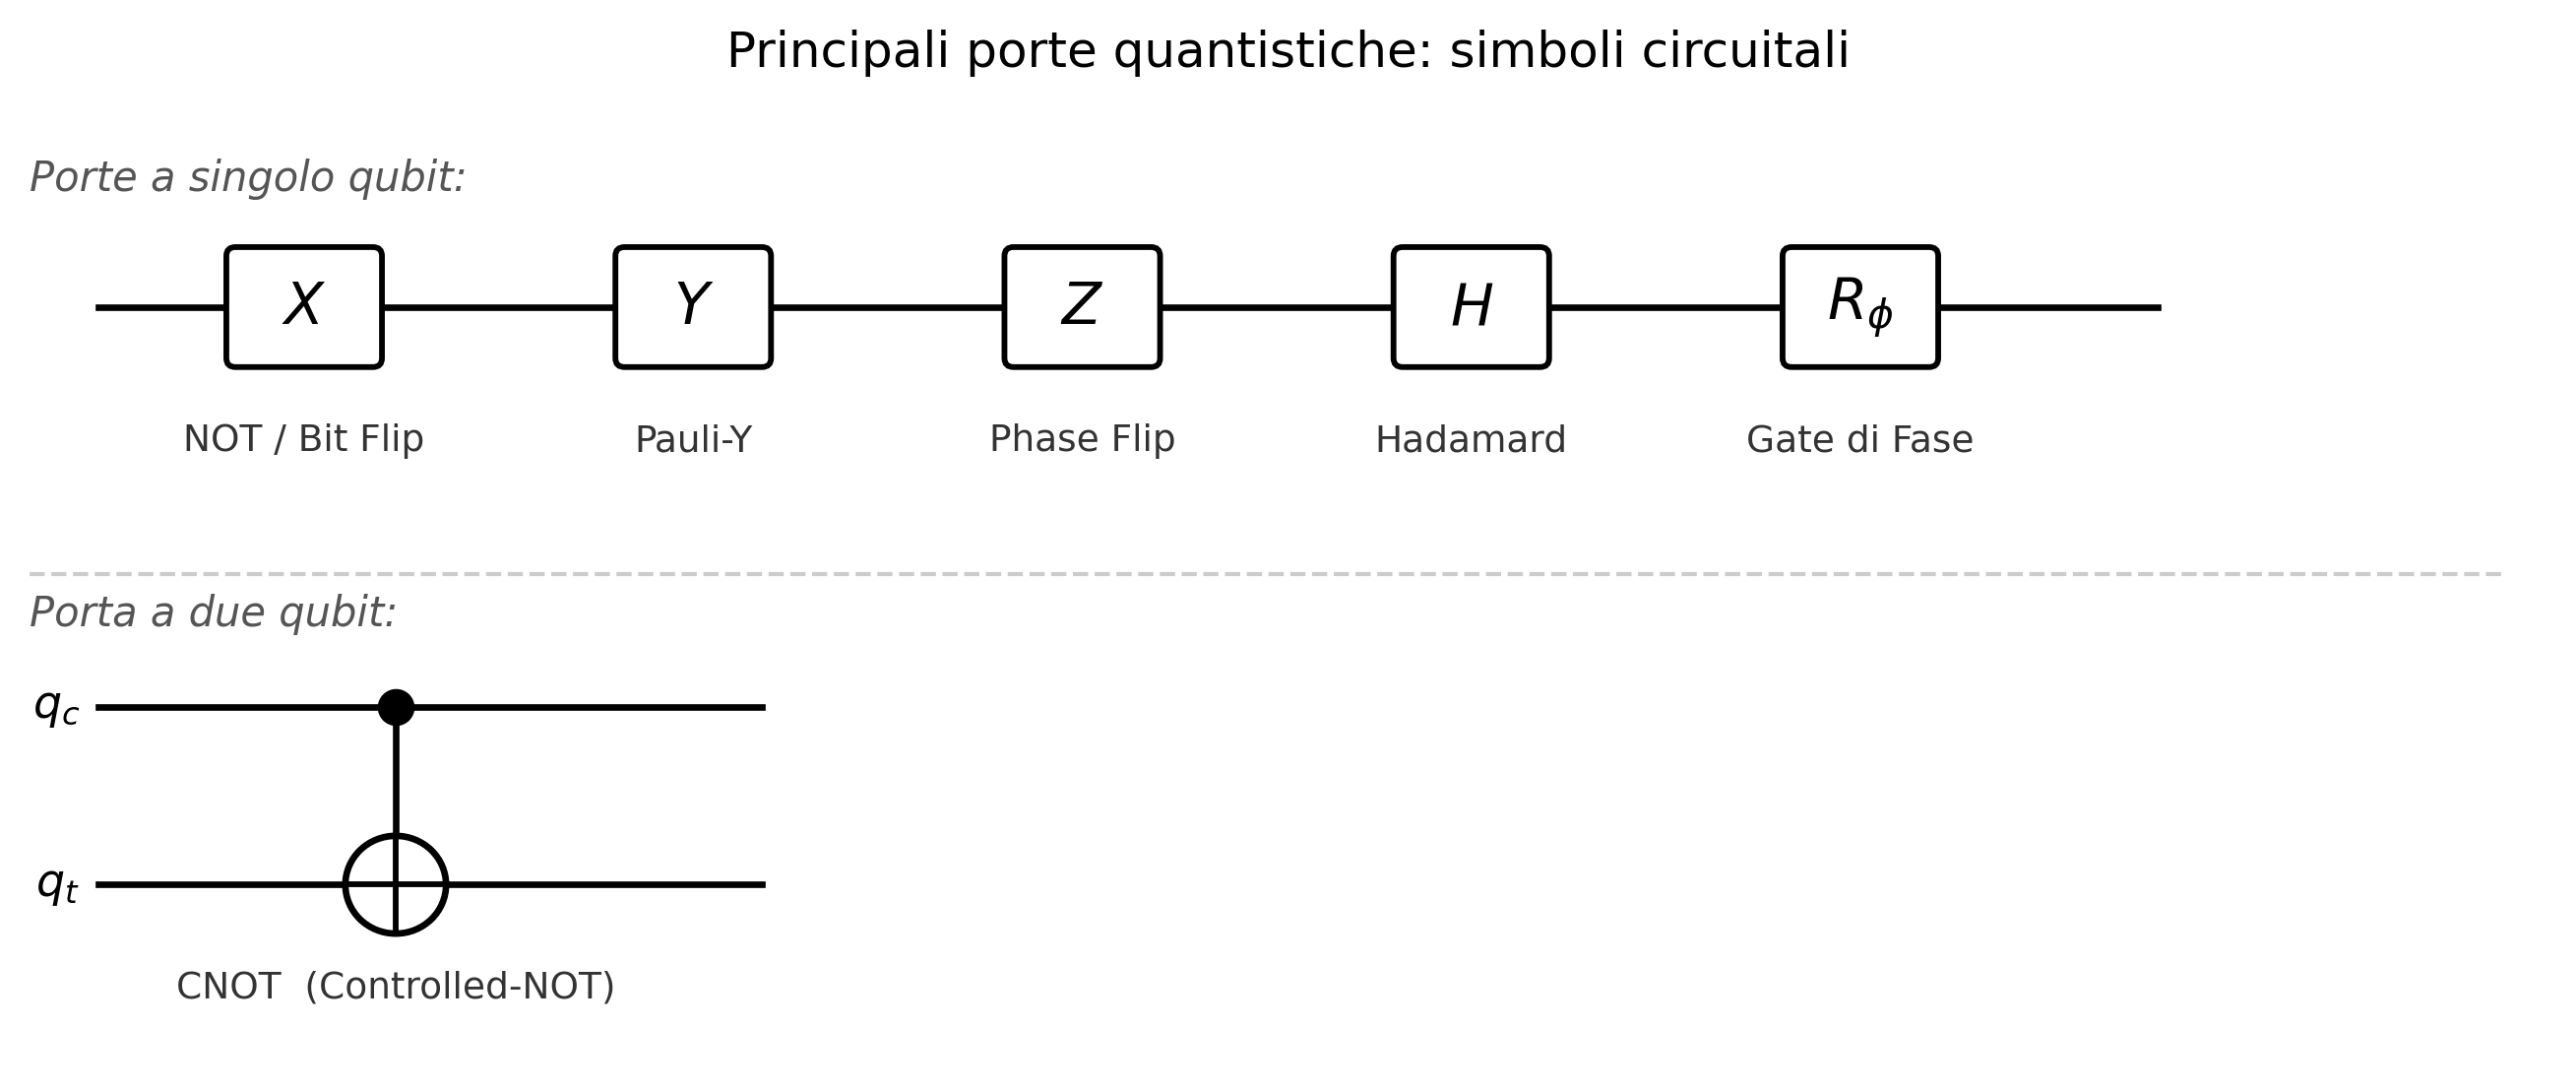
\includegraphics[width=0.88\textwidth]{circuit_gates.png}

\caption[Porte quantistiche a singolo e due qubit]{Simboli circuitali delle principali porte quantistiche a singolo qubit ($X$, $Y$, $Z$, $H$, $R_\phi$) e della porta CNOT a due qubit. Nella porta CNOT, il punto pieno indica il qubit di controllo $q_c$ e il cerchio con croce indica il qubit target $q_t$.}\label{fig:gates}
\end{figure}
\clearpage
\subsection{Circuiti Quantistici}

Un \textbf{circuito quantistico} è una sequenza ordinata di porte quantistiche applicata a un registro di qubit. I circuiti si leggono da sinistra a destra, con ogni filo orizzontale che rappresenta l'evoluzione temporale di un qubit. La composizione di porte corrisponde al prodotto matriciale degli operatori unitari associati.

L'equivalente quantistico del teorema di universalità classico afferma che qualunque trasformazione unitaria su $n$ qubit può essere \textbf{approssimata con precisione arbitraria} da una sequenza finita di porte prese da un insieme universale, tipicamente $\{H, T, \text{CNOT}\}$. La distinzione fra approssimazione e decomposizione esatta non è pedanteria: le sequenze finite su un insieme di porte fissato sono numerabili, mentre le trasformazioni unitarie non lo sono, sicché una decomposizione esatta è impossibile in generale. Il teorema di Solovay--Kitaev garantisce che l'approssimazione a precisione $\varepsilon$ richiede $O(\log^c(1/\varepsilon))$ porte, con $c$ costante piccola: il costo dell'approssimazione cresce dunque solo polilogaritmicamente, ed è questa la ragione per cui l'universalità resta praticamente utile.

\subsection{Interferenza Quantistica}

Poiché la misura distrugge le ampiezze (Postulato~3), gli algoritmi quantistici devono amplificare la risposta corretta \emph{prima} della misura.

L'\textbf{interferenza} è il meccanismo fondamentale attraverso cui gli algoritmi quantistici realizzano il loro vantaggio computazionale. Le ampiezze quantistiche sono numeri complessi e possono combinarsi costruttivamente (quando hanno lo stesso segno/fase) o distruttivamente (quando hanno fase opposta).

Un algoritmo quantistico efficiente è costruito in modo che:
\begin{itemize}
    \item Le ampiezze degli stati \textbf{sbagliati} si cancellino per \textbf{interferenza distruttiva};
    \item Le ampiezze degli stati \textbf{corretti} si sommino per \textbf{interferenza costruttiva}.
\end{itemize}

Questo meccanismo è alla base sia dell'algoritmo di Grover sia dell'algoritmo di Shor (Capitolo~\ref{chap:shor}), dove la Quantum Fourier Transform realizza l'interferenza necessaria al ritrovamento del periodo.

\subsection{Modello di Complessità Quantistica}

La complessità di un algoritmo quantistico è misurata in termini di numero di porte (equivalente delle operazioni elementari classiche) e di profondità del circuito (numero di livelli di porte parallele). La classe centrale è \ac{BQP}, che contiene i problemi risolvibili da un computer quantistico in tempo polinomiale con probabilità di errore al più $1/3$.

Le inclusioni $\mathbf{P} \subseteq \mathbf{BPP} \subseteq \mathbf{BQP} \subseteq \mathbf{PSPACE}$ sono \emph{dimostrate}; ciò che resta aperto è se siano \textbf{strette}. Non è noto se BQP contenga propriamente P o BPP --- cioè se esista davvero un problema che un computer quantistico risolva efficientemente e uno classico no --- né se sia propriamente contenuto in PSPACE. Una dimostrazione di separazione stretta fra BQP e BPP implicherebbe $\mathbf{P} \neq \mathbf{PSPACE}$, un risultato che la teoria della complessità non ha ancora raggiunto: è questa la ragione per cui il vantaggio quantistico, per Shor come per gli altri algoritmi, resta una congettura ampiamente creduta e non un teorema.

\begin{figure}[H]
    \centering
    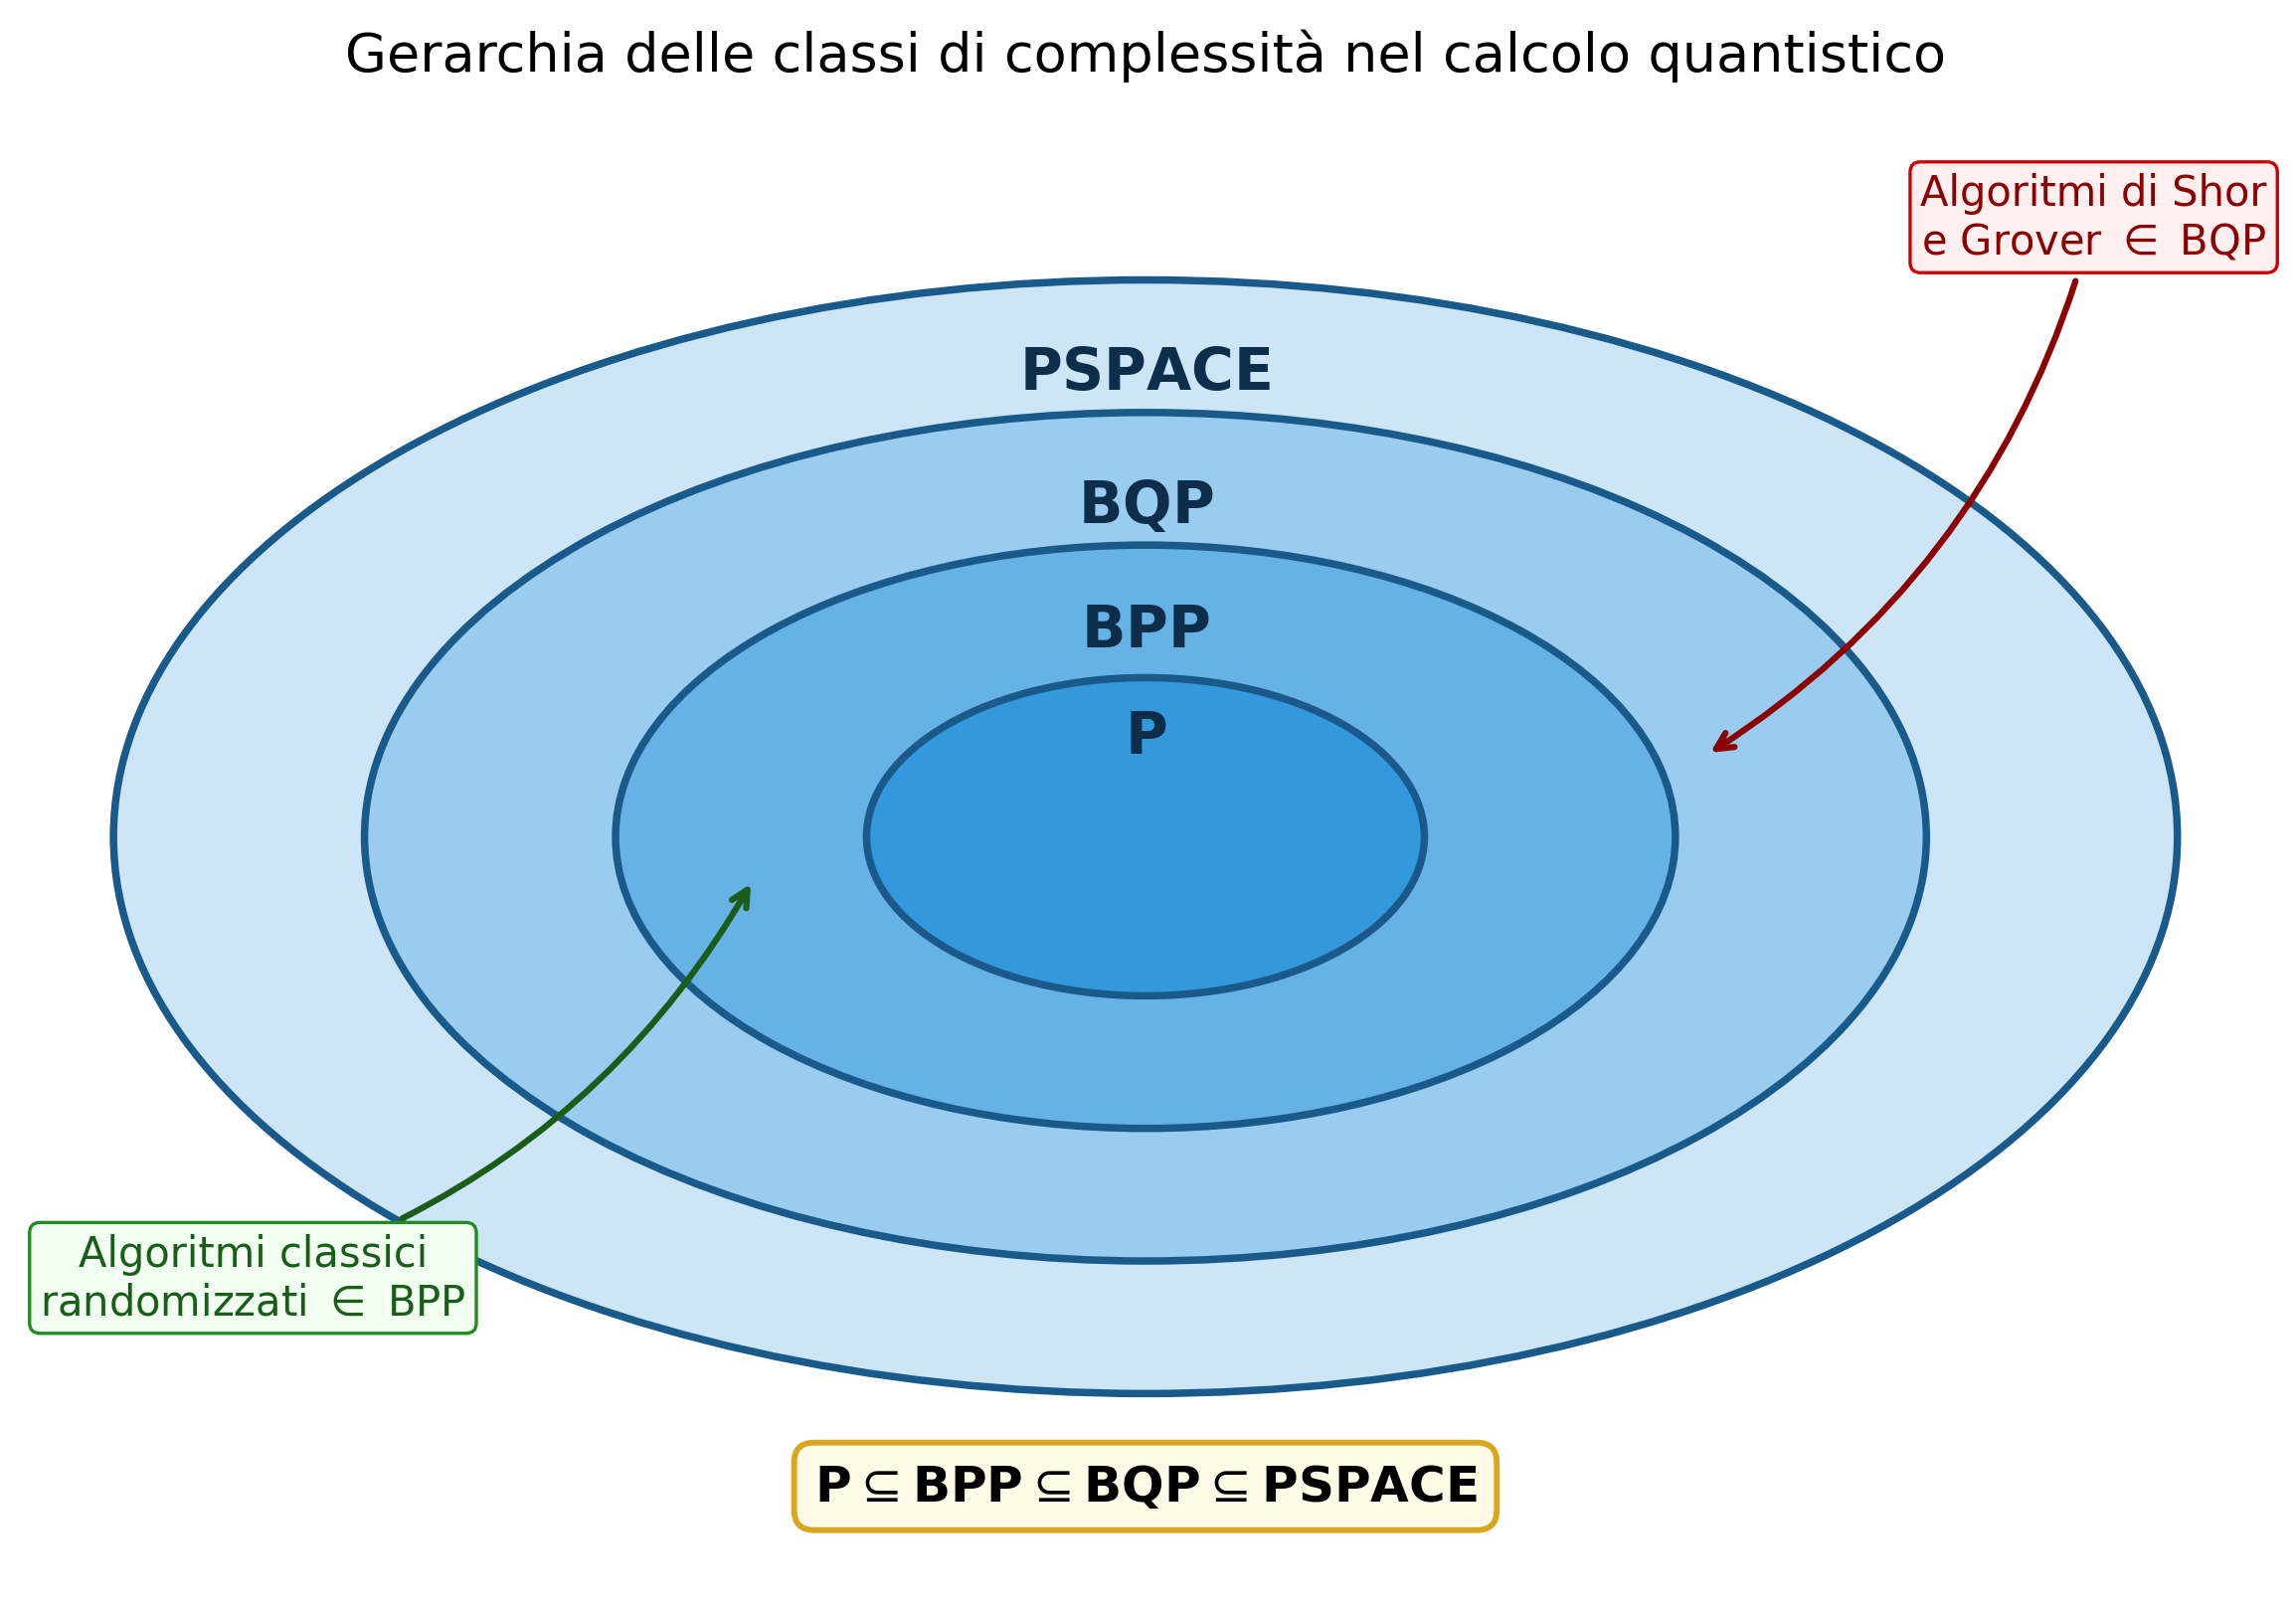
\includegraphics[width=0.68\textwidth]{complexity_classes.png}

\caption[Gerarchia delle classi di complessità quantistica]{Gerarchia delle classi di complessità nel calcolo quantistico. La classe BQP cattura i problemi efficientemente risolvibili da un computer quantistico; le inclusioni mostrate ($\mathrm{P} \subseteq \mathrm{BPP} \subseteq \mathrm{BQP} \subseteq \mathrm{PSPACE}$) sono dimostrate, mentre è congetturata --- e non dimostrata --- la loro \emph{strettezza}. Gli algoritmi di Shor e Grover risiedono in BQP; che la fattorizzazione non appartenga a P è ritenuto probabile ma non provato.}\label{fig:complexity}
\end{figure}

\end{onehalfspace}


\section{L'anatomia fisica di una QPU}
\label{app:anatomia}

Il Capitolo~\ref{chap:rumore} isola di questa materia i soli tre fatti che ricorrono nel
seguito; questa sezione ne d\`a la trattazione completa.

\subsection{Qubit, Controllo e Vincoli Fisici della QPU}

Per capire dove nascono gli errori bisogna prima capire com'è fatta la macchina. Una \ac{QPU} superconduttiva è un chip criogenico che contiene \emph{esclusivamente} i qubit e le linee fisiche che li collegano: contrariamente all'intuizione, \textbf{le porte logiche non risiedono nel chip}. Aprendo una CPU classica si trovano registri e porte logiche incise nel silicio; aprendo una QPU si trovano solo i qubit. Le operazioni sono realizzate dall'\textbf{elettronica di controllo esterna}, che invia impulsi a microonde convogliati ai qubit tramite guide d'onda: ``far passare un qubit in un gate'' significa in realtà inviargli un impulso sagomato che ne ruota lo stato sulla sfera di Bloch dell'angolo desiderato (90°, 30°, 10°, \ldots). La Figura~\ref{fig:qpu_anatomia} schematizza questa architettura per una QPU a 5 qubit con topologia a catena lineare.

\begin{figure}[H]
\centering
\begin{tikzpicture}[
  qubit/.style={circle, draw=black, thick, fill=blue!15, minimum size=9mm, font=\small},
  testq/.style={circle, draw=black, thick, dashed, fill=gray!15, minimum size=9mm, font=\small},
  wave/.style={decorate, decoration={snake, amplitude=0.5mm, segment length=2.4mm}, thick, <->, >=stealth, orange!80!black},
  coupl/.style={line width=1.6pt, gray!60}
]
\node[rectangle, draw=black, thick, fill=orange!12, minimum width=112mm, minimum height=11mm, align=center, font=\small] (E) at (4.4, 3.1)
  {\textbf{Elettronica di controllo e lettura} (temperatura ambiente)\\[-1mm] {\footnotesize è qui che ``vivono'' i gate: impulsi a microonde sagomati}};
\draw[rounded corners=3mm, thick, fill=blue!3] (-1.1,-1.9) rectangle (12.2,1.0);
\node[font=\footnotesize\itshape, anchor=south west] at (-1.0,-1.85) {chip criogenico ($\sim$15 mK) --- la QPU vera e propria};
\node[qubit] (Q0) at (0,0) {$Q_0$};
\node[qubit] (Q1) at (2.2,0) {$Q_1$};
\node[qubit] (Q2) at (4.4,0) {$Q_2$};
\node[qubit] (Q3) at (6.6,0) {$Q_3$};
\node[qubit] (Q4) at (8.8,0) {$Q_4$};
\draw[coupl] (Q0) -- (Q1);
\draw[coupl] (Q1) -- (Q2);
\draw[coupl] (Q2) -- (Q3);
\draw[coupl] (Q3) -- (Q4);
\node[font=\footnotesize, gray!50!black] at (4.4,-0.75) {accoppiatori fisici: entanglement diretto solo tra qubit \emph{adiacenti}};
\node[testq] (T0) at (11.2,0.2) {$T_0$};
\node[font=\scriptsize, align=center, gray!30!black] at (11.2,-1.0) {qubit di riferimento\\non accoppiato\\ai qubit dati};
\foreach \q in {Q0,Q1,Q2,Q3,Q4}{ \draw[wave] (E.south -| \q) -- (\q.north); }
\node[font=\footnotesize, orange!60!black, align=center] at (11.0,2.0) {microonde:\\controllo $\downarrow$ / lettura $\uparrow$};
\end{tikzpicture}

\caption[Anatomia schematica di una QPU superconduttiva a 5 qubit]{Schema didattico di una \ac{QPU} superconduttiva: cinque qubit in catena, qubit di riferimento $T_0$ ed elettronica esterna di controllo e lettura.}\label{fig:qpu_anatomia}
\end{figure}

Schema didattico di una \ac{QPU} superconduttiva a 5 qubit con topologia a catena. Nel chip criogenico risiedono qubit, risonatori e accoppiatori; le operazioni sono pilotate dall'elettronica esterna mediante linee di controllo e lettura. L'interazione a due qubit diretta è disponibile solo lungo gli accoppiamenti disegnati ($Q_1$--$Q_2$ sì, $Q_0$--$Q_2$ mediante routing). $T_0$ rappresenta un qubit di riferimento non accoppiato alla catena, ma ancora dotato delle linee necessarie a preparazione e misura: non fornisce una misura ``pura'' di $T_1$ e non elimina perdite, Purcell effect o altre sorgenti di decoerenza.


La Figura~\ref{fig:qpu_reale} mostra come questa architettura si presenta nella realtà: all'esterno il sistema integrato (criostato, elettronica e schermature racchiusi nella teca), all'interno della sala macchine i cilindri criogenici sospesi con il fascio di tubi e cavi coassiali che convogliano le microonde di controllo e lettura --- le ``guide d'onda'' dello schema precedente.

\begin{figure}[!htbp]
\centering
\subfloat[IBM Quantum System One]{\begin{minipage}{0.48\textwidth}\centering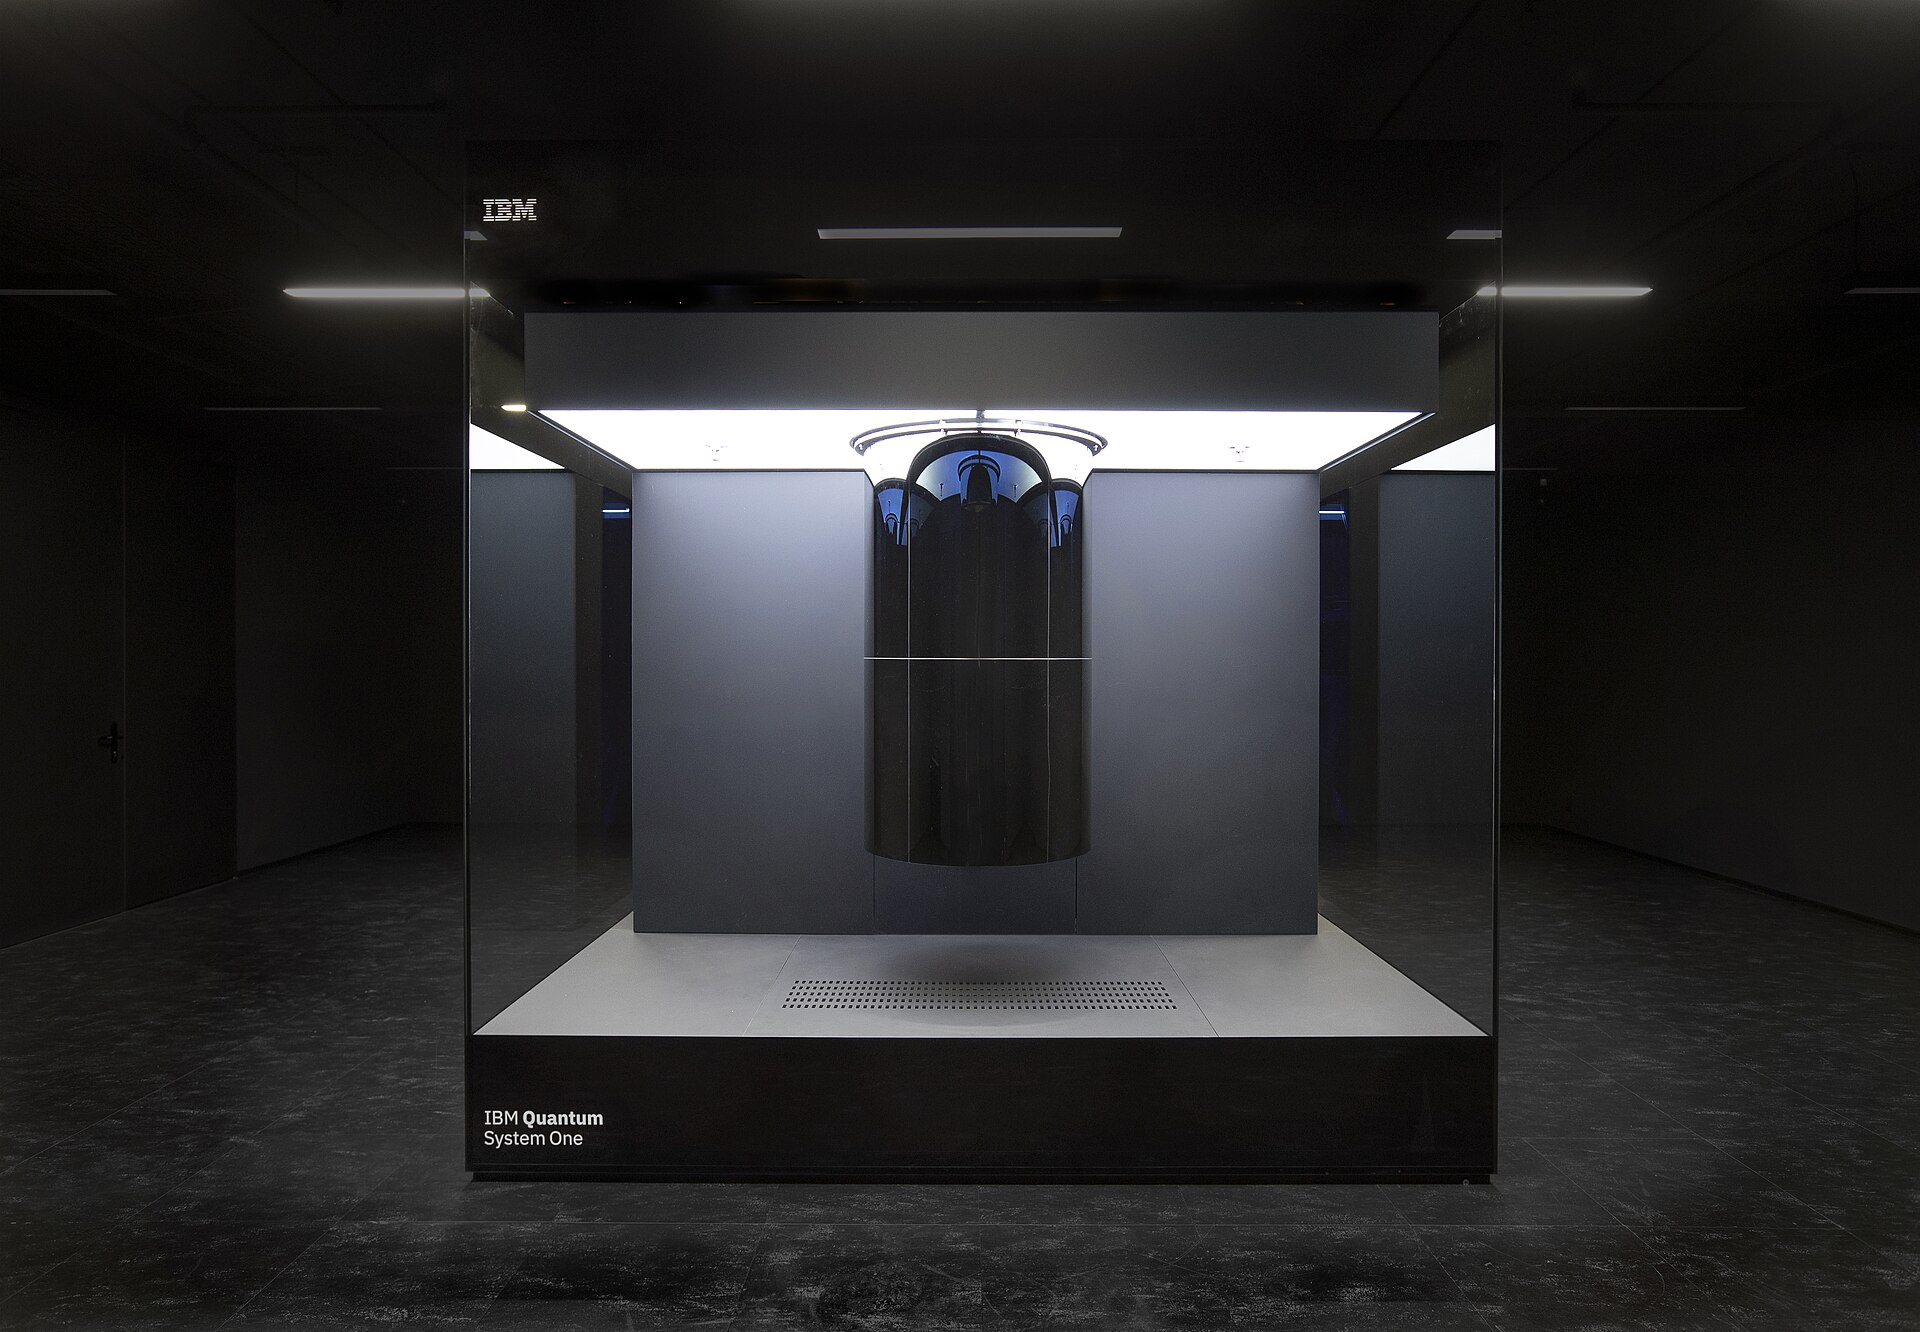
\includegraphics[width=\linewidth,height=36mm,keepaspectratio]{foto_system_one.jpg}\end{minipage}}\hfill
\subfloat[Criostati e cablaggio]{\begin{minipage}{0.48\textwidth}\centering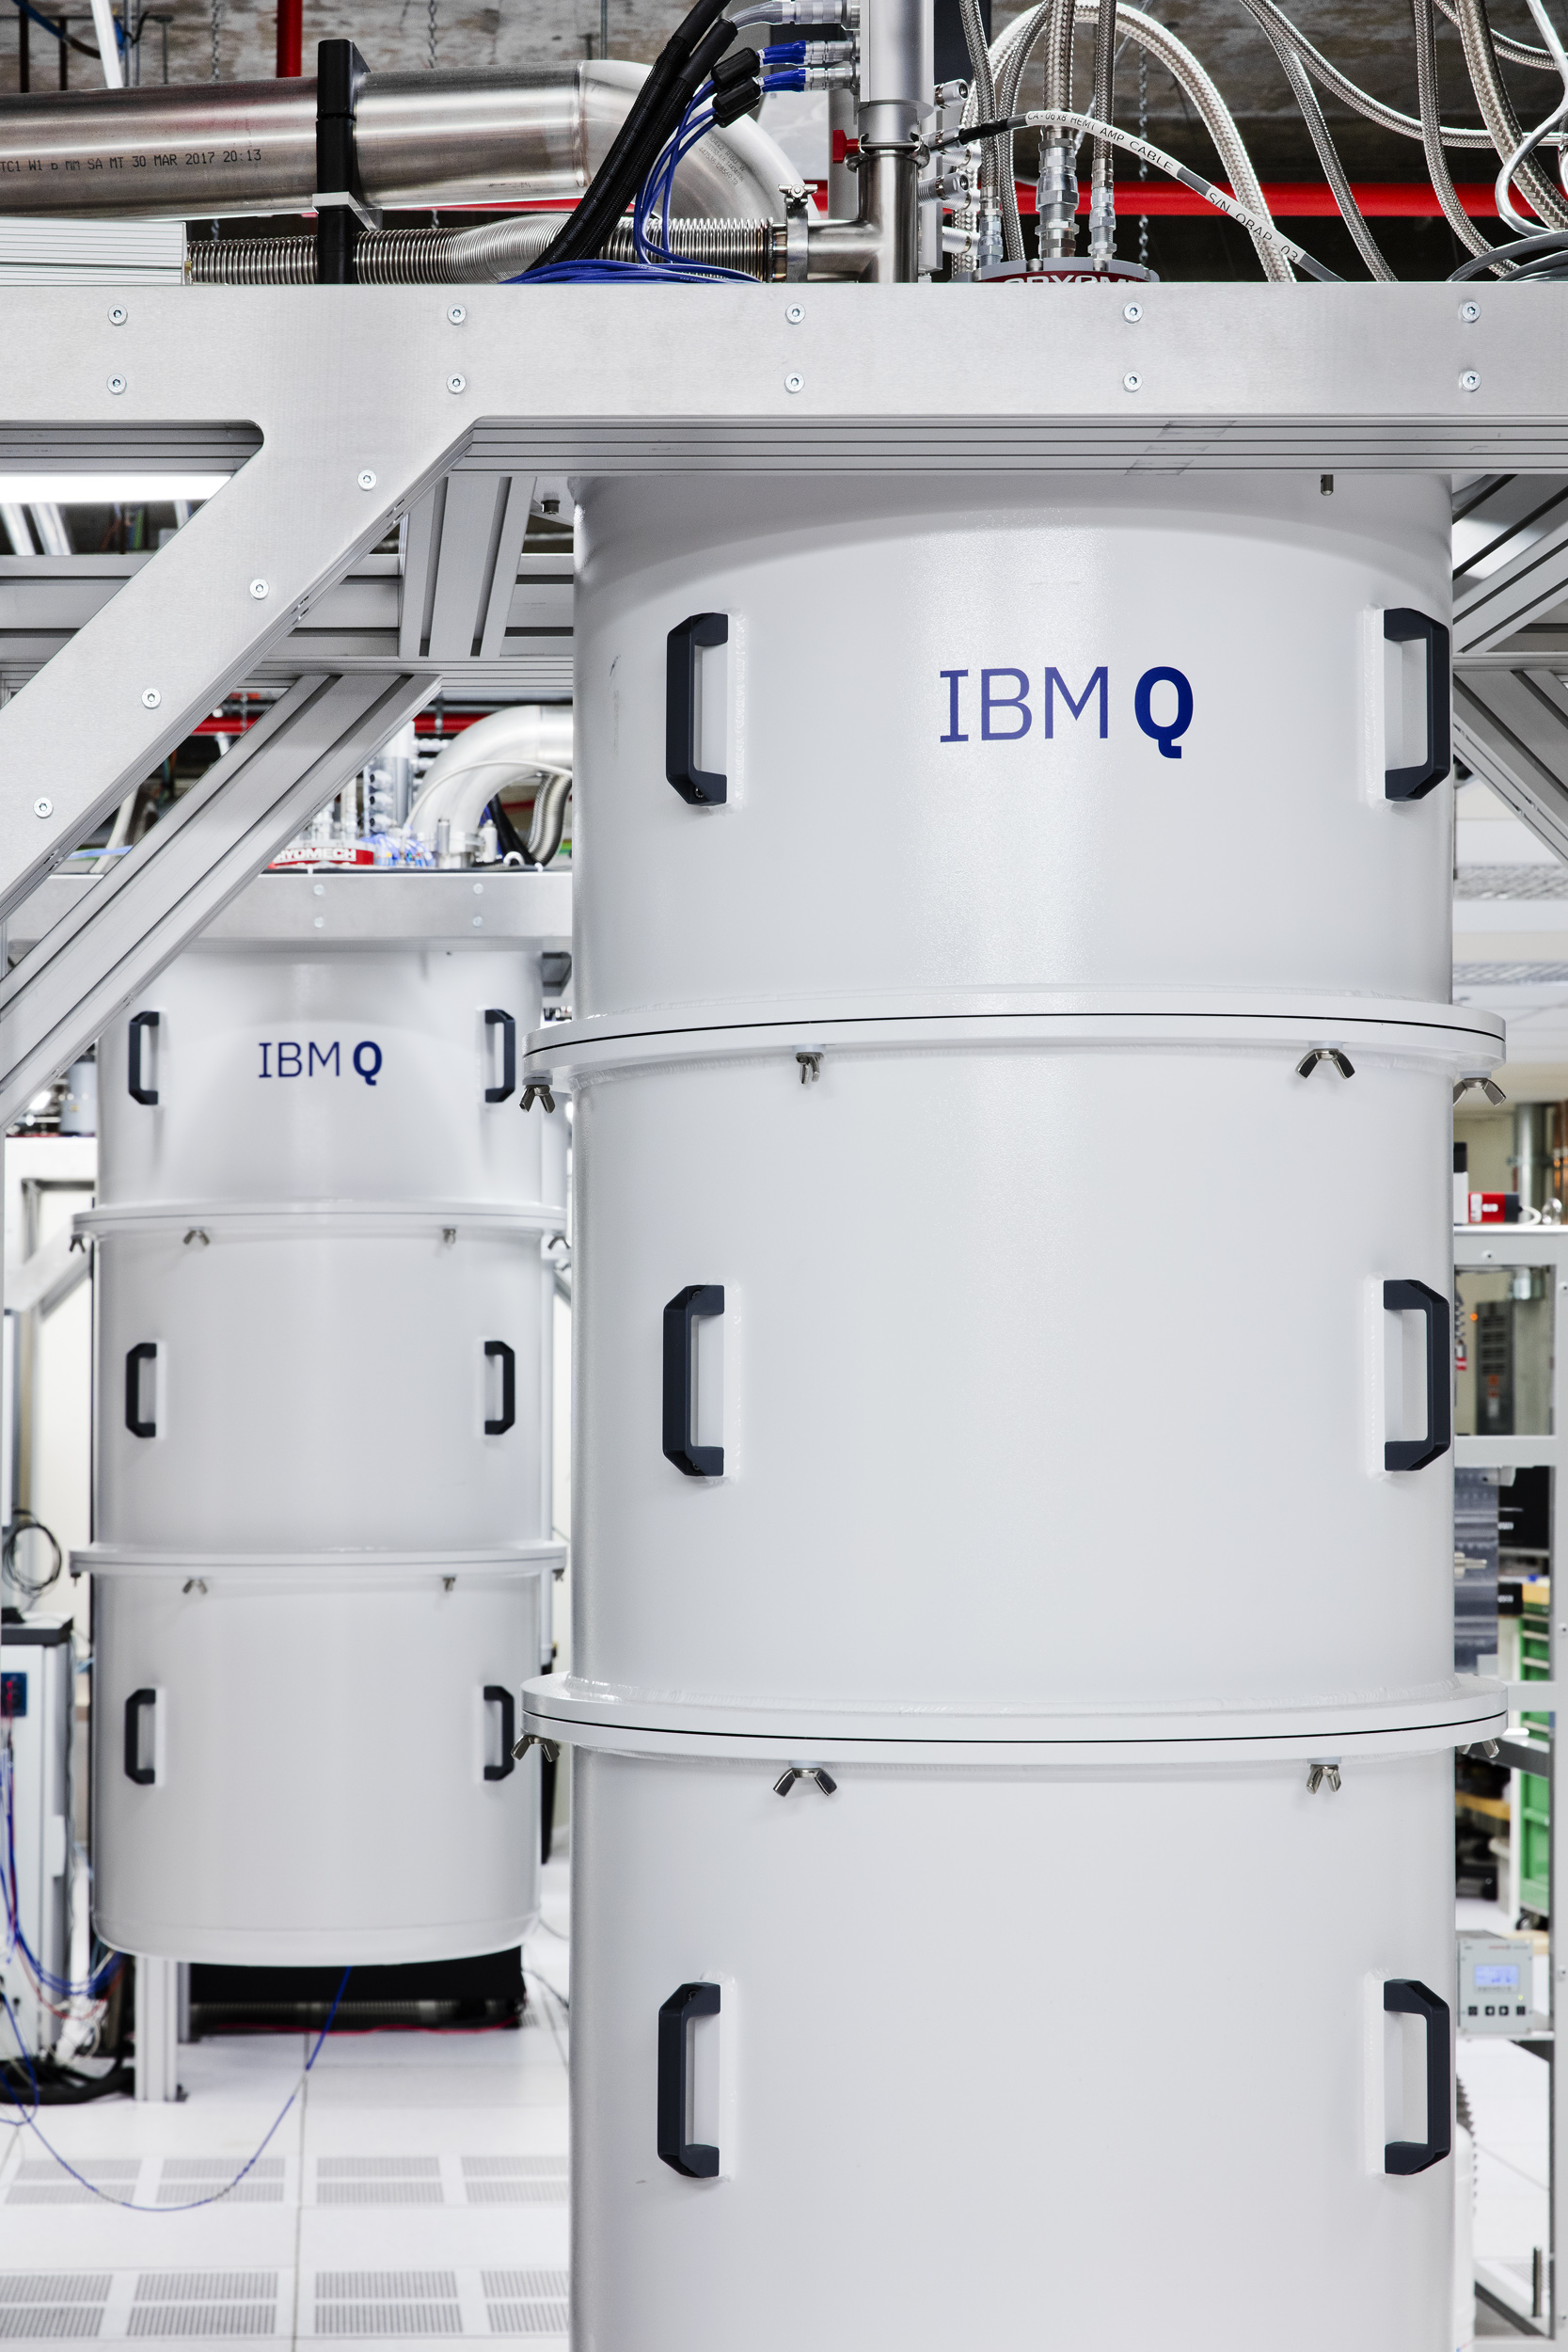
\includegraphics[width=\linewidth,height=36mm,keepaspectratio]{foto_criostato_ibm.jpg}\end{minipage}}

\caption[La QPU reale: sistema integrato e criostati con cablaggio]{IBM Quantum System One (a) e criostati IBM Q con cablaggio di controllo (b). Crediti: IBM Research, CC~BY~2.0 (a); Connie Zhou per IBM, pubblico dominio (b), via Wikimedia Commons.}\label{fig:qpu_reale}
\end{figure}

La \ac{QPU} reale. (a)~Il sistema integrato IBM Quantum System One: il cilindro nero al centro è il criostato che contiene il chip, circondato dall'elettronica di controllo. (b)~Criostati IBM Q in sala macchine: dall'alto arrivano i tubi per la refrigerazione e i cavi coassiali che convogliano le microonde di controllo e lettura verso il chip, sospeso sul fondo del cilindro a $\sim$15\,mK.


\begin{figure}[!htbp]
\centering
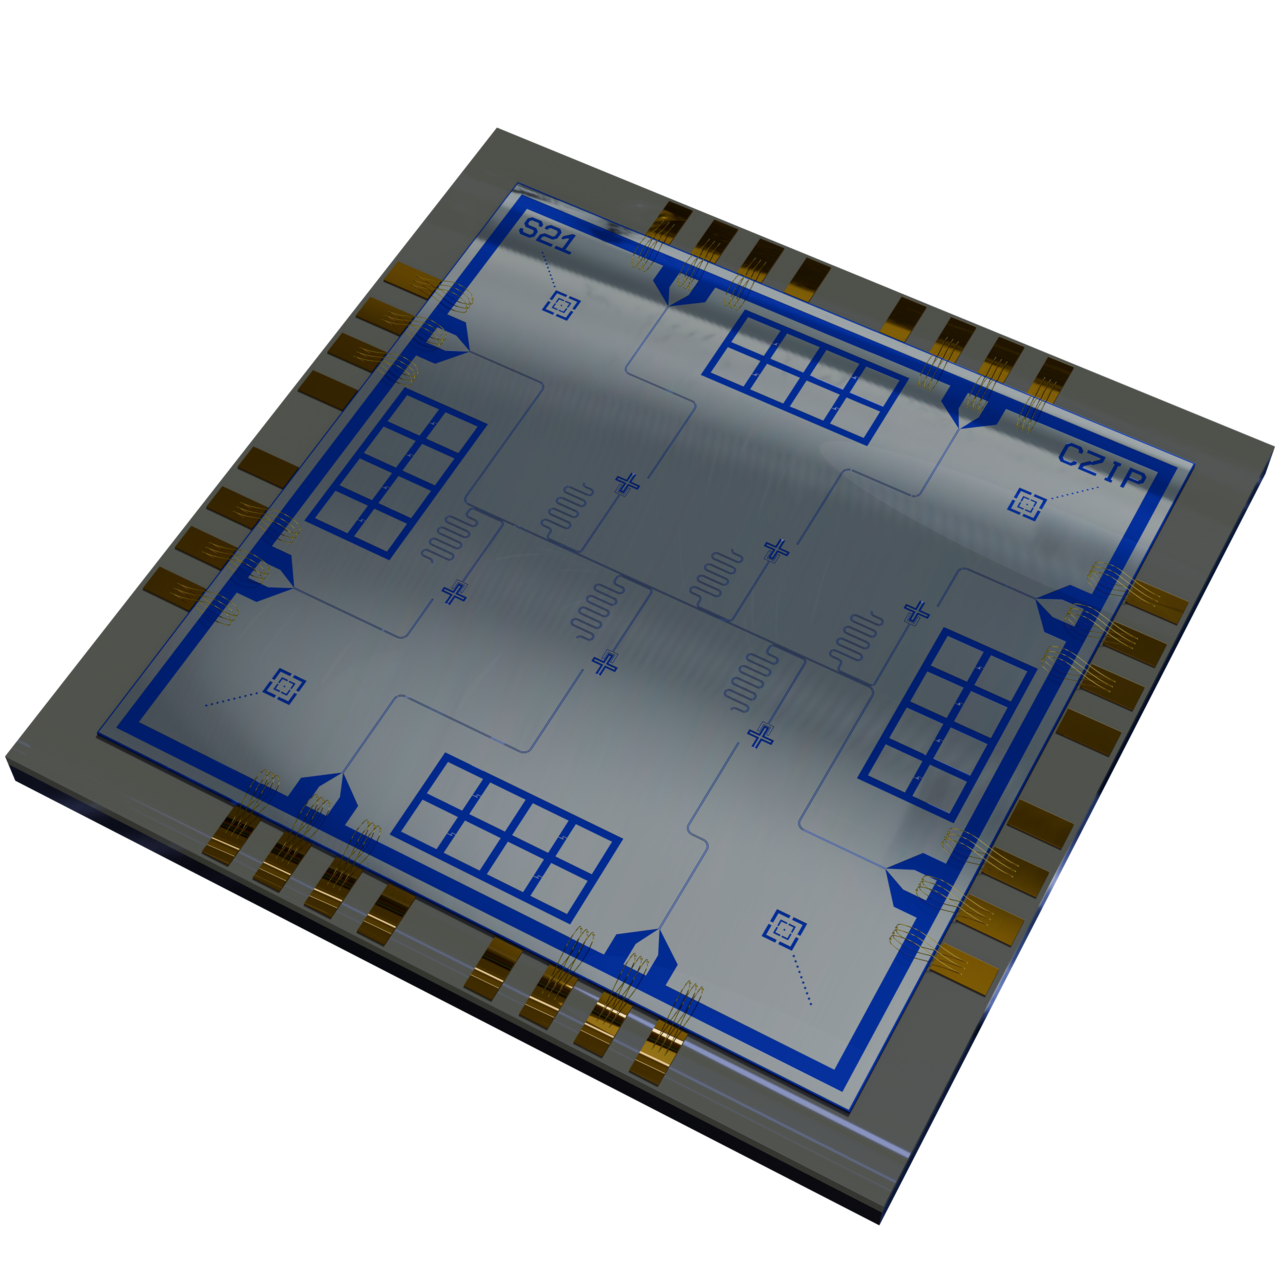
\includegraphics[width=0.48\textwidth,height=0.25\textheight,keepaspectratio]{foto_chip_transmon.png}

\caption[Chip quantistico superconduttivo a 6 transmon con giunzioni di test]{Resa tridimensionale di un chip a sei transmon e dodici giunzioni di test. Credito: Onri Jay Benally, CC~BY~4.0, via Wikimedia Commons.}\label{fig:chip_transmon}
\end{figure}

Resa tridimensionale di un chip quantistico superconduttivo con 6 qubit transmon e 12 giunzioni di test. Si riconoscono gli elementi dello schema di Figura~\ref{fig:qpu_anatomia}: i qubit con i loro risonatori, le linee di accoppiamento, le piazzole dorate per il collegamento alle guide d'onda e --- ai quattro angoli --- le strutture di test isolate, l'analogo reale del qubit $T_0$.


Questa architettura ha tre conseguenze dirette per gli errori.

\paragraph{La lettura distrugge lo stato - fisicamente.}
Anche la misura avviene tramite microonde: ogni qubit è accoppiato a un risonatore, si invia un impulso di sonda al risonatore e se ne osserva la risposta, che cambia a seconda che il qubit sia in $\ket{0}$ o in $\ket{1}$ (lettura dispersiva). L'interazione con la sonda fa collassare lo stato del qubit misurato: il collasso del Postulato~3 è un processo fisico, non soltanto una regola matematica. Il segnale di lettura può inoltre disturbare i qubit vicini; per questo le misure a metà circuito richiedono calibrazioni dedicate e, nei circuiti di questa tesi, tutte le misure sono collocate alla fine.

\paragraph{Il budget di operazioni: coerenza vs velocità dei gate.}
Le prestazioni di una QPU dipendono dal rapporto tra due tempi: quanto a lungo il qubit resta coerente e quanto dura una singola operazione. Con una finestra di coerenza di $100\,\mu$s e gate da $\sim$25\,ns, si eseguono $\sim$4\,000 operazioni; una macchina con coerenza superiore ma gate più lenti può eseguirne \emph{meno}. È il rapporto che conta, non il singolo parametro --- ed è questo rapporto a decidere se il circuito di Shor per una data istanza è fisicamente eseguibile. La Tabella~\ref{tab:tecnologie_qpu} confronta gli ordini di grandezza delle due principali tecnologie.

\begin{table}[H]
\centering

\small
\begin{tabularx}{\textwidth}{@{}lXX@{}}
\toprule
 & \textbf{Superconduttori (IBM, IQM, \ldots)} & \textbf{Ioni intrappolati (IonQ, Quantinuum, \ldots)} \\
\midrule
Tempo di coerenza          & $50$--$300\,\mu$s                      & da secondi a minuti \\
\addlinespace[0.3em]
Durata gate (1 qubit)      & $\sim$15--40\,ns                       & $\sim$1--100\,$\mu$s \\
\addlinespace[0.3em]
Durata gate (2 qubit)      & $\sim$60--500\,ns                      & $\sim$0.1--1\,ms \\
\addlinespace[0.3em]
Operazioni per finestra    & $\sim 10^{3}$--$10^{4}$                & $\sim 10^{3}$ \\
\addlinespace[0.3em]
Lettura                    & più esposta a errori e interferenze     & più stabile e affidabile \\
\addlinespace[0.3em]
Crosstalk                  & presente (accoppiamento capacitivo)     & ridotto \\
\addlinespace[0.3em]
Velocità di esecuzione     & molto alta                              & bassa (gate lenti) \\
\bottomrule
\end{tabularx}
\caption[Confronto tra tecnologie di QPU: superconduttori vs ioni intrappolati]{Ordini di grandezza indicativi delle due principali tecnologie di \ac{QPU}. La coerenza lunghissima degli ioni intrappolati non si traduce in più operazioni utili, perché i gate sono da $10^3$ a $10^4$ volte più lenti: il budget di operazioni per finestra di coerenza è simile, ma i superconduttori lo spendono molto più in fretta. Gli ioni sono invece più robusti su lettura e crosstalk.}\label{tab:tecnologie_qpu}

\end{table}

\paragraph{La durata del circuito conta.}
La perdita di coerenza si accumula con il tempo: per un decadimento esponenziale con costante $T$, la probabilità che il qubit abbia perso l'informazione dopo un tempo $t$ è $1-e^{-t/T}$, che cresce con continuità al crescere di $t$. Non esiste quindi una soglia netta oltre la quale il calcolo fallisce, ma un circuito che occupa una frazione rilevante di $\min(T_1,T_2)$, come quello di Shor, arriva alla misura con una probabilità d'errore elevata anche se la sua durata è formalmente inferiore ai tempi di coerenza.

\paragraph{La topologia decide chi parla con chi.}
Le QPU differiscono anche per geometria: catene lineari, griglie (heavy-hex di IBM), connettività completa. Su una catena, una porta fra qubit non adiacenti richiede di avvicinare l'informazione con porte SWAP attraverso i qubit intermedi: ogni SWAP costa tre porte a due qubit, e quindi tempo ed errori aggiuntivi. La topologia determina quindi sia \emph{quali} circuiti si possono mappare in modo efficiente, sia \emph{dove} il crosstalk colpirà. Questo aspetto --- insieme al fatto che i parametri di coerenza variano da qubit a qubit dello stesso chip --- è ripreso nel Capitolo~\ref{chap:surface}, dove la località delle interazioni sulla griglia è il fondamento architetturale del surface code.

\subsection{Le quattro fonti fisiche: parametri e modelli di misura}
\label{app:fonti_fisiche_estese}

Questa sottosezione completa la Sezione~\ref{sec:fonti_fisiche} con formule,
ordini di grandezza e limiti interpretativi.

\subsubsection{Decoerenza: rilassamento e perdita di fase}

La \textbf{decoerenza} nasce dall'interazione con campi elettromagnetici
parassiti, fononi e fluttuazioni termiche. Il \textbf{tempo di rilassamento}
$T_1$ descrive il decadimento spontaneo da $\ket{1}$ a $\ket{0}$ per
dissipazione energetica; su dispositivi superconduttori è tipicamente
dell'ordine di $50$--$500\,\mu$s. Il \textbf{tempo di dephasing} $T_2$
descrive invece la randomizzazione della fase relativa e combina rilassamento e
perdita pura di fase:
\begin{equation}
    \frac{1}{T_2}=\frac{1}{2T_1}+\frac{1}{T_\phi},
    \label{eq:T2_decomp}
\end{equation}
dove $T_\phi$ è il tempo di puro dephasing; vale $T_2\leq2T_1$ e sono comuni
ordini di grandezza di $50$--$200\,\mu$s.

Sul cammino critico, il criterio
\begin{equation}
    \tau_{\text{circuito}}\ll\min(T_1,T_2)
\end{equation}
è soltanto euristico. La crescita polinomiale dell'aritmetica non determina una
soglia universale in bit: compilazione, parallelismo, idle, topologia e QEC
fissano la durata fisica effettiva. In particolare, durante la phase estimation
la coerenza di fase deve sostenere l'entanglement fra i registri; confrontare
$T_2/\tau_{\text{gate}}$ con il numero totale di porte sarebbe scorretto perché
un conteggio non è una durata. Per questo il noise model usa durate esplicite e
riporta separatamente conteggi e profondità.

\subsubsection{Errori di gate}

Un gate fisico realizza $\widetilde U=U+\delta E$ anziché $U$. Una misura
ideale della discrepanza è la gate infidelity
\begin{equation}
 r(U,\widetilde U)=1-F(U,\widetilde U),\qquad
 F(U,\widetilde U)=\frac{1}{d^2}
 \left|\operatorname{Tr}(U^\dagger\widetilde U)\right|^2.
\end{equation}
Le cause includono errori di ampiezza o frequenza degli impulsi, accoppiamento
\emph{always-on} e leakage verso livelli non computazionali
($\ket{2},\ket{3},\ldots$). Gli ordini indicativi 2024--2025 sono
$r\simeq0.03$--$0.1\%$ per gate 1Q e $0.3$--$1\%$ per gate 2Q; non sono
assunti come calibrazione delle campagne di questa tesi.

\subsubsection{Readout e crosstalk}

Il readout è descritto da una matrice di confusione
\begin{equation}
 A_{ij}=P(\text{misura }i\mid\text{stato }j),\qquad
 \sum_iA_{ij}=1.
\end{equation}
Sotto l'ipotesi d'indipendenza, per $n$ qubit vale
$A=\bigotimes_{k=1}^nA_k$, con
\begin{equation}
 A_k=\begin{pmatrix}
 1-e_0^{(k)}&e_1^{(k)}\\ e_0^{(k)}&1-e_1^{(k)}
 \end{pmatrix},
\end{equation}
dove $e_0^{(k)}$ è la probabilità di leggere $1$ dato $\ket{0}$; valori
indicativi sono $1$--$3\%$.

Il \textbf{crosstalk} è invece l'interferenza fra operazioni simultanee su
qubit vicini, dovuta soprattutto all'accoppiamento capacitivo residuo. Produce
rotazioni parassite, dipende dalla topologia ed è difficile da modellare
analiticamente~\cite{sarovar2020}. Proprio le correlazioni spaziali non
rappresentate nel grafo del decoder costituiscono, nella
Sezione~\ref{sec:decodifica_appresa}, il regime in cui il correttore residuo
appreso mostra un guadagno rispetto al riferimento analitico.


\section{L'algoritmo di Shor - approfondimenti e stato dell'arte}
\label{app:shor_esteso}

Questa sezione approfondisce l'algoritmo di Shor presentato nel Capitolo~\ref{chap:shor}: lo stato delle realizzazioni sperimentali, i miglioramenti algoritmici recenti, la sensibilità delle sue componenti al rumore e il perimetro delle istanze studiate.

\subsection{Sviluppi Recenti e Stato dell'Arte}

\subsubsection{Implementazioni su Hardware Reale}

Nonostante la solidità teorica, l'esecuzione di Shor su hardware reale rimane limitata a istanze molto piccole a causa dei requisiti di profondità circuitale. I principali risultati sperimentali sono:

\begin{itemize}
    \item \textbf{2001 -- \ac{NMR} (Vandersypen et al.)}: prima dimostrazione sperimentale di Shor su un sistema a 7 spin nucleari; fattorizzazione di $N = 15$ in $3 \times 5$ \cite{vandersypen2001}.
    \item \textbf{2016 -- Ioni intrappolati (Monz et al.)}: implementazione scalabile su 5 qubit ionici; fattorizzazione di $N = 15$ con un'architettura modulare \cite{monz2016}.
    \item \textbf{2021 -- Qubit superconduttori \ac{IBM}}: dimostrazione compilata della fattorizzazione di $N = 21$ su processori \ac{IBM} Quantum utilizzando 5 qubit \cite{skosana2021}.
\end{itemize}

Queste istanze evidenziano quanto la distanza dalle chiavi crittograficamente rilevanti sia ancora enorme. Una stima classica del fabbisogno, formulata sul modello di circuito privo di correzione d'errore, riporta $5K+1$ qubit di memoria e circa $72K^3$ gate elementari per fattorizzare un numero di $K$ bit \cite{beckman1996}; costanti e overhead dipendono però dall'architettura aritmetica e, nelle stime moderne, dal protocollo fault-tolerant, rispetto al quale quel conteggio va inteso come limite inferiore ottimistico. In ogni caso, i valori per RSA-2048 restano fuori portata per i processori \ac{NISQ} attuali.

Alla distanza teorica se ne aggiunge una operativa, documentata da una campagna recente su più piattaforme cloud: le costruzioni circuitali restano specifiche per ciascun modulo, e le fedeltà delle macchine si presentano instabili, con tassi d'errore elevati e fluttuanti \cite{shor_challenges2025}. È la ragione per cui, in questo lavoro, $N=15$ è trattato come istanza illustrativa e non come misura di fattibilità.

\subsubsection{Miglioramenti Algoritmici: Regev 2023}

Un risultato teorico rilevante è stato pubblicato nel 2023 da Oded Regev \cite{regev2023}. La proposta fattorizza un intero di $n$ bit eseguendo indipendentemente circa $\sqrt n+4$ circuiti, ciascuno con $\widetilde O(n^{3/2})$ gate, seguiti da post-processing classico polinomiale. Il confronto con Shor non può quindi essere ridotto al solo conteggio di gate di una singola esecuzione: aumentano il numero di run e, nella costruzione originale, anche lo spazio quantistico; inoltre l'articolo dichiara non chiaro l'effettivo vantaggio implementativo. Il risultato è un miglioramento asintotico importante, non una dimostrazione di praticabilità su dispositivi NISQ.

\subsection{Sensibilità delle componenti di Shor al rumore}
\label{app:shor_rumore_esteso}

La seguente analisi completa la parte sul rumore del Capitolo~\ref{chap:quadro}
con derivazioni, esempio numerico e figura di scala.

\subsubsection{Errori nella Quantum Fourier Transform}

La \ac{QFT} usa rotazioni
$R_k=\operatorname{diag}(1,e^{2\pi i/2^k})$ con angoli esponenzialmente
piccoli. Per $k=10$, $2\pi/1024\simeq6\times10^{-3}$ rad. Gli errori coerenti
di calibrazione possono sommarsi in ampiezza, mentre il canale depolarizzante
produce degradazione stocastica: non è quindi corretto ricondurli a un solo
``errore di fase'' lineare. Le campagne li mantengono distinti.

\subsubsection{Errori nella Phase Estimation}

I qubit di controllo devono mantenere la coerenza lungo il cammino critico
dell'esponenziazione modulare. Come ordine di grandezza,
\begin{equation}
    T_2\gg\tau_{\text{gate}}\,O(n^3),
\end{equation}
con i limiti discussi nella Sezione~\ref{app:fonti_fisiche_estese}; in regime
fault-tolerant il confronto diretto è sostituito da un budget di errore logico.

\subsubsection{Errori nell'esponenziazione modulare}

Sotto l'ipotesi puramente illustrativa di $L$ eventi indipendenti con
probabilità $\epsilon$, il proxy di nessun evento è
\begin{equation}
    P_{0\text{-eventi}}=(1-\epsilon)^L,\qquad L\sim O(n^3).
\end{equation}
Ponendo soltanto per visualizzare la scala $L=n^3$, per $n=15$ e
$\epsilon=10^{-3}$ si ottiene
$(1-10^{-3})^{3375}\simeq0.034$. Non è una probabilità di successo di Shor:
alcuni errori possono non alterare l'esito e la formula non rappresenta
rilassamento, readout o struttura circuitale.

\begin{figure}[H]
\centering
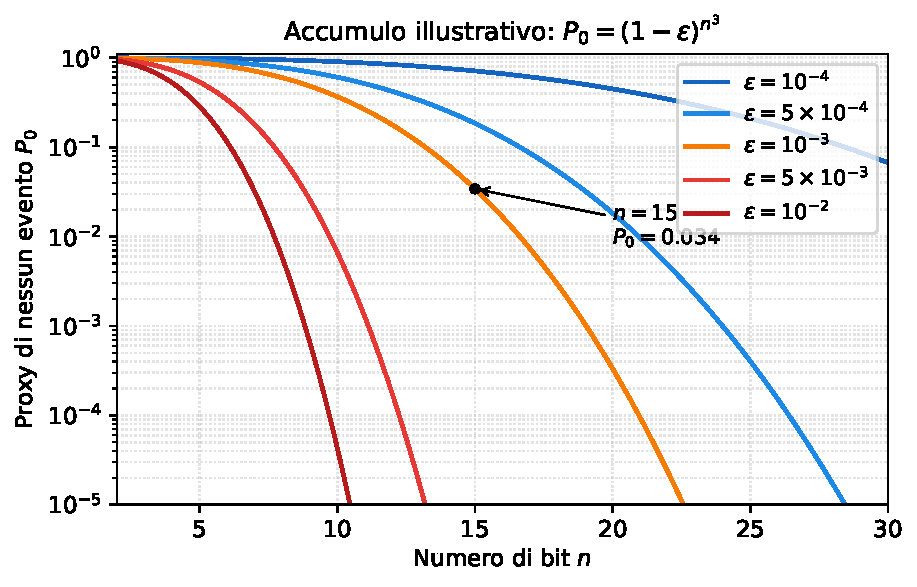
\includegraphics[width=0.74\textwidth,height=0.30\textheight,keepaspectratio]{15_psuccess_vs_n.pdf}

\caption[Proxy di nessun evento al crescere del circuito]{Proxy illustrativo
$(1-\epsilon)^{n^3}$ per cinque valori di $\epsilon$. La curva non deriva dai
circuiti sperimentali e mostra soltanto l'accumulo moltiplicativo di eventi.}\label{fig:psuccess_vs_n}
\end{figure}

\subsection{Scelta dell'aritmetica e perimetro delle istanze}
\label{app:shor_perimetro_esteso}

Sintetizzare l'esponenziazione modulare come un operatore unitario denso costa
$O(4^k)$ porte elementari su $k$ qubit~\cite{Barenco1995}. La decomposizione
di Beauregard~\cite{beauregard2002} evita tale sintesi costruendo l'aritmetica
nel dominio della \ac{QFT}, con addizionatori di Draper, e richiede
$O(n^3)$ porte su $2n+3$ qubit. Il costo resta elevato: per $N=21$, $a=2$ e
otto qubit di conteggio, la compilazione congiunta in
\texttt{rz/sx/x/cx} produce 21\,036 porte \ac{CX} e profondità 23\,081.
Il costo dominante non è la trasformata finale della \ac{QPE}, ma le
trasformate interne agli addizionatori; è lì che l'approssimazione deve agire
per incidere sul conteggio di porte.

Le campagne rumorose sono perciò limitate a $N=15$, $a=7$; le istanze
$N=21$ e $N=35$ sono validate solo idealmente (Sezione~\ref{app:fase1_contratto}).

In termini di spazio, fattorizzare un intero di $n$ bit richiede almeno
$2n$ qubit logici per la phase estimation, oltre alle ancille necessarie
all'aritmetica modulare. Il conteggio non include l'overhead fault-tolerant e
non basta a stimare la fattibilità: connettività e routing possono aumentare
profondità e numero di porte senza modificare il numero di qubit logici.


\section{I canali di rumore: derivazioni complete}
\label{app:canali}

I quattro canali quantistici che modellano il rumore sono mappe \ac{CPTP} in
rappresentazione di Kraus, secondo il formalismo richiamato nella
Sezione~\ref{sec:finale_3_1_3}. Il Capitolo~\ref{chap:rumore} ne riporta il
canale depolarizzante per esteso, essendo quello su cui poggia la campagna
sperimentale, e l'enunciato compatto degli altri tre; qui se ne danno le
derivazioni complete.

\subsection{Canale Bit Flip}

Il canale \textbf{bit flip} modella un errore di tipo $X$ discreto: con probabilità $p$ il qubit viene invertito ($\ket{0}\leftrightarrow\ket{1}$), con probabilità $1-p$ rimane invariato. Gli operatori di Kraus sono $K_0 = \sqrt{1-p}\,I$ e $K_1 = \sqrt{p}\,X$, e il canale agisce come:
\begin{equation}
    \mathcal{E}_{BF}(\rho) = (1-p)\,\rho + p\,X\rho X
    \label{eq:bitflip}
\end{equation}
Sulla sfera di Bloch, le componenti $r_y$ e $r_z$ vengono contratte di un fattore $(1-2p)$ mentre la componente $r_x$ rimane invariata. Per $p=1/2$ il canale annulla le componenti $y$ e $z$, ma conserva $r_x$: equivale a una completa dephasing nella base degli autostati di $X$, non alla distruzione completa dello stato.

\subsection{Canale Phase Flip}

Il canale \textbf{phase flip} modella la perdita di informazione di fase senza cambiamento di popolazione: la sovrapposizione decade senza che l'energia venga dissipata. Con operatori di Kraus $K_0 = \sqrt{1-p}\,I$ e $K_1 = \sqrt{p}\,Z$, il canale è:
\begin{equation}
    \mathcal{E}_{PF}(\rho) = (1-p)\,\rho + p\,Z\rho Z
    \label{eq:phaseflip}
\end{equation}
L'effetto sulla matrice densità è immediato:
\begin{equation}
    \mathcal{E}_{PF}\!\begin{pmatrix}\rho_{00} & \rho_{01} \\ \rho_{10} & \rho_{11}\end{pmatrix}
    = \begin{pmatrix}\rho_{00} & (1-2p)\,\rho_{01} \\ (1-2p)\,\rho_{10} & \rho_{11}\end{pmatrix}
\end{equation}
Le popolazioni $\rho_{00}$ e $\rho_{11}$ rimangono invariate, mentre le \textbf{coerenze} $\rho_{01}$, $\rho_{10}$ vengono soppresse di un fattore $(1-2p)$. Questo è il canale che descrive il decadimento $T_2$: parametrizzando $p(t) = \frac{1}{2}(1-e^{-t/T_2})$, si ottiene $\rho_{01}(t) = \rho_{01}(0)\,e^{-t/T_2}$.

\subsection{Canale di Amplitude Damping}

Il canale di \textbf{amplitude damping} modella il rilassamento energetico $T_1$: il qubit decade spontaneamente dallo stato eccitato $\ket{1}$ allo stato fondamentale $\ket{0}$ con probabilità $\gamma = 1-e^{-t/T_1}$. Gli operatori di Kraus sono:
\begin{equation}
    K_0 = \begin{pmatrix}1 & 0 \\ 0 & \sqrt{1-\gamma}\end{pmatrix}, \qquad
    K_1 = \begin{pmatrix}0 & \sqrt{\gamma} \\ 0 & 0\end{pmatrix}
    \label{eq:kraus_ad}
\end{equation}
Il canale agisce sulla matrice densità come:
\begin{equation}
    \mathcal{E}_{AD}\!(\rho) = \begin{pmatrix}
        \rho_{00} + \gamma\,\rho_{11} & \sqrt{1-\gamma}\,\rho_{01} \\
        \sqrt{1-\gamma}\,\rho_{10}   & (1-\gamma)\,\rho_{11}
    \end{pmatrix}
    \label{eq:amp_damping_explicit}
\end{equation}
La popolazione $\rho_{11}$ decade verso $\rho_{00}$ con tasso $\gamma$, mentre le coerenze vengono soppresse di $\sqrt{1-\gamma}$. A differenza dei canali precedenti, questo canale è \textbf{non simmetrico}: sulla sfera di Bloch contrae la sfera verso il polo nord $\ket{0}$, non verso il centro:
\begin{equation}
    r_x \to \sqrt{1-\gamma}\,r_x, \qquad r_y \to \sqrt{1-\gamma}\,r_y, \qquad r_z \to (1-\gamma)\,r_z + \gamma
\end{equation}
Per $t \to \infty$ ($\gamma \to 1$), qualsiasi stato converge a $\ket{0}\bra{0}$, indipendentemente dallo stato iniziale.

\subsection{Confronto geometrico dei quattro canali}

La visualizzazione seguente mostra che canali con probabilità d'errore simili
possono produrre geometrie molto diverse nello spazio degli stati.

Per il canale depolarizzante, l'identità
$X\rho X+Y\rho Y+Z\rho Z=2I-\rho$ (per $\operatorname{Tr}\rho=1$) conduce
dalla forma a miscela di Pauli alla forma compatta discussa nella
Sezione~\ref{sec:finale_3_3_2}. Il vettore di Bloch è moltiplicato per
$1-4p/3$ e, per $p=3/4$, lo stato diventa massimamente misto qualunque fosse
l'ingresso. Nel parametro Aer $\lambda$, invece, la probabilità aggregata di
una Pauli non identità è $3\lambda/4$ su un qubit e $15\lambda/16$ su due.
I preset uniformi compongono depolarizzazione e thermal relaxation; M8 usa il
solo proxy Pauli per gate, mentre M11 converte l'infedeltà media della snapshot
senza aggiungere nuovamente $T_1/T_2$, evitando il doppio conteggio.

\begin{figure}[H]
\centering
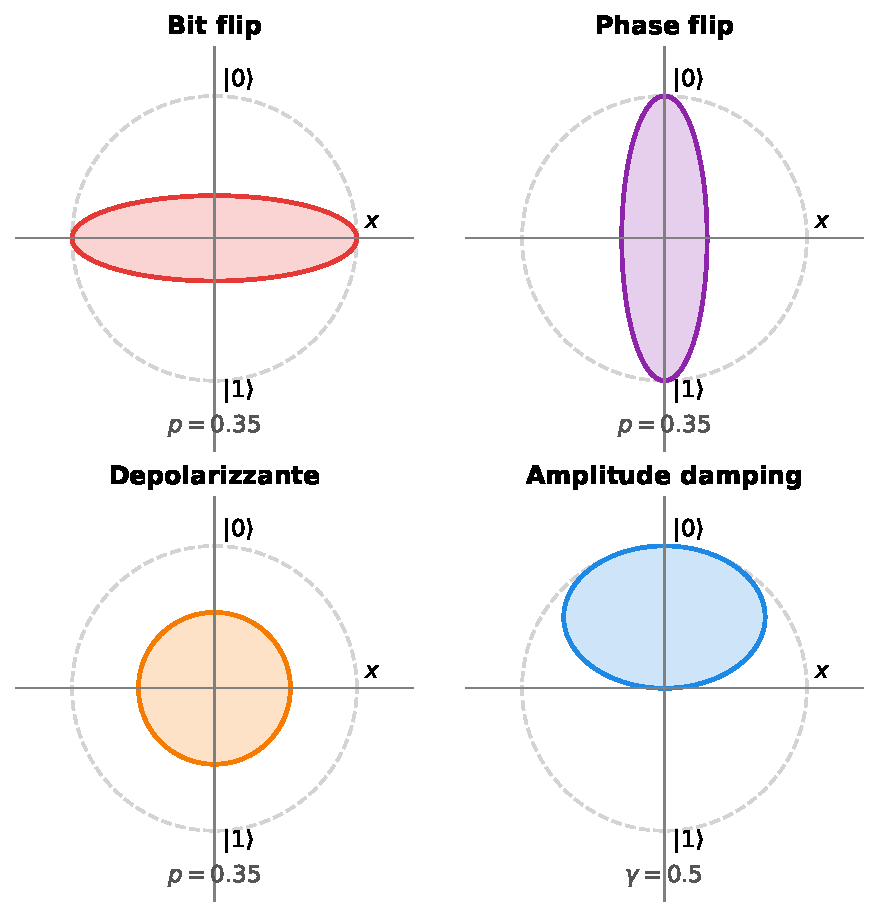
\includegraphics[width=0.78\textwidth,height=0.37\textheight,keepaspectratio]{14_bloch_channels.pdf}

\caption[Effetto dei canali di rumore sulla sfera di Bloch]{Effetto dei quattro
canali nel piano $xz$. La curva tratteggiata è la sfera ideale: bit flip e
phase flip contraggono direzioni selettive, il depolarizzante contrae
isotropicamente e l'amplitude damping sposta lo stato verso $\ket{0}$.}\label{fig:bloch_channels}
\end{figure}

\begin{table}[H]
\centering
\small

\begin{tabular}{@{}llll@{}}
\toprule
\textbf{Canale} & \textbf{Effetto sulle coerenze} & \textbf{Popolazioni} & \textbf{Modella} \\
\midrule
Bit flip & contrae $r_y,r_z$ & scambiate & errore $X$ \\
\addlinespace[0.3em]
Phase flip & sopprime $\rho_{01}$ & invariate & dephasing $T_2$ \\
\addlinespace[0.3em]
Depolarizzante & contrazione isotropa & verso $I/2$ & gate generico \\
\addlinespace[0.3em]
Amplitude damping & sopprime $\rho_{01}$ & verso $\ket{0}$ & rilassamento $T_1$ \\
\bottomrule
\end{tabular}
\caption{Confronto fra i quattro canali fondamentali~\cite{nielsenChuang2000}.}\label{tab:canali_rumore}

\end{table}

\section{Strategie anti-rumore e richiami estesi di QEC}
\label{app:strategie_estese}

Questa sezione completa la parte del Capitolo~\ref{chap:quadro} dedicata alle
strategie anti-rumore con rassegna, esempi e confronti estesi.

\subsection{I quattro livelli di intervento}

\begin{enumerate}
    \item \textbf{Soppressione del rumore.} Agisce prima o durante il calcolo
    riducendo fisicamente l'accoppiamento con l'ambiente. Comprende
    \emph{dynamical decoupling}, ottimizzazione della durata dei gate e
    isolamento criogenico ed elettromagnetico. Riduce il rumore ma è vincolata
    all'hardware disponibile.

    \item \textbf{Mitigazione degli errori.} Opera a posteriori senza
    correggere i qubit. \ac{ZNE}, \emph{probabilistic error cancellation} e
    gate twirling combinano più esecuzioni o randomizzazioni per stimare
    l'output ideale. Il limite è l'overhead di campionamento, la cui legge
    dipende dalla tecnica e può diventare esponenziale nell'errore totale,
    soprattutto per la PEC.

    \item \textbf{Tolleranza ai guasti.} Codifica ogni qubit logico in molti
    qubit fisici. Sotto le ipotesi del threshold theorem e al di sotto della
    soglia~\cite{aharonov1997fault}, l'errore logico può essere ridotto
    aumentando distanza e overhead. Le stime per algoritmi di grande scala
    possono richiedere centinaia o migliaia di qubit fisici per qubit logico,
    a seconda di codice, errore fisico e obiettivo.

    \item \textbf{Metodi appresi.} Modelli classici possono classificare
    output, stimare qualità o assistere un decoder. Non sono automaticamente
    \ac{QML}, né sostituiscono per definizione mitigazione o QEC.
\end{enumerate}

Nel perimetro della tesi la soppressione non è controllabile, la mitigazione
richiede esecuzioni aggiuntive e la fault tolerance completa eccede le risorse
disponibili. Un modello a valle non modifica il circuito, ma il suo vantaggio è
un'ipotesi da confrontare con regole semplici. Per questo TOP-1, TOP-4 e M2
usano gli stessi istogrammi, mentre la \ac{ZNE} è un controllo secondario.

\subsection{Usi possibili dei metodi appresi}

Il termine appropriato per gli esperimenti è \textbf{machine learning classico
applicato a dati quantistici}: Random Forest, \ac{SVM} e \ac{MLP} sono
addestrati ed eseguiti classicamente. Il \ac{QML} in senso stretto impiega
circuiti o modelli quantistici nell'apprendimento e non è implementato. Tre usi
distinti chiariscono il perimetro:
\begin{itemize}
    \item nella \textbf{caratterizzazione del rumore}, una regressione può
    collegare $T_1,T_2$, profondità e fedeltà per predire la qualità;
    \item nell'\textbf{ottimizzazione circuitale}, un agente può adattare
    decomposizione e routing al profilo d'errore del dispositivo;
    \item nella \textbf{decodifica QEC}, un modello usa le sindromi per
    proporre una correzione o correggere residualmente una decisione analitica.
\end{itemize}
Il terzo caso colloca il machine learning \emph{dentro una fase} della QEC,
senza ridefinire la disciplina.

\subsection{Principio, codici e decoder QEC}
\label{app:qec_richiami_teoria}

Il no-cloning impedisce di proteggere un qubit duplicandolo, ma non di
\emph{distribuire} l'informazione logica su più qubit fisici. Misurando
operatori collettivi si ottiene una sindrome dell'errore senza rivelare, e
quindi distruggere, lo stato logico. Il paradigma comprende:
\begin{enumerate}
    \item codifica di $\ket{\psi_L}$ su $n$ qubit fisici;
    \item misura di stabilizzatori che commutano con i codeword e
    anticommutano con determinate classi d'errore;
    \item decodifica della sindrome e scelta dell'operazione di recupero.
\end{enumerate}

Il \textbf{codice di Shor}~\cite{shorcorrection1995} codifica un qubit in nove
e corregge un errore singolo arbitrario:
\begin{equation}
 \ket{0_L}=\frac{(\ket{000}+\ket{111})^{\otimes3}}{2\sqrt2},\qquad
 \ket{1_L}=\frac{(\ket{000}-\ket{111})^{\otimes3}}{2\sqrt2}.
\end{equation}
La struttura combina protezione dalla fase mediante interferenza e dal bit flip
mediante ripetizione. Il \textbf{codice di Steane}~\cite{steane1996} usa sette
qubit e la struttura del codice classico di Hamming $[7,4,3]$; è un codice
\ac{CSS}~\cite{calderbankShor1996} e corregge anch'esso un errore singolo. Il
\textbf{surface code}~\cite{fowler2012} dispone invece i qubit su una griglia
2D con interazioni locali: sotto una soglia dipendente da circuito, rumore e
decoder, aumentare la distanza $d$ sopprime l'errore logico; sopra soglia lo
amplifica.

Il punto di contatto con il machine learning è la decodifica
\cite{torlaiMelko2017,alphaqubit2024}. Un modello può sostituire il decoder o
intervenire sui suoi residui, ma deve essere confrontato a parità di sindromi e
calendario. Nel protocollo studiato la sostituzione del matching non conviene;
l'affiancamento recupera invece una parte degli errori correlati assenti dal
grafo analitico. Questo è un risultato circoscritto al modello simulato, non una
superiorità generale dei decoder appresi.

\subsection{AQFT e scambio fra qubit e porte}
\label{app:aqft_estesa}

La \ac{QFT} impiega rotazioni controllate con angolo esponenzialmente più
piccolo all'aumentare della distanza fra qubit. L'\ac{AQFT} scarta quelle sotto
una soglia: perde precisione algoritmica, ma riduce il conteggio di porte. Per
$N=21$, troncare le trasformate interne agli addizionatori porta le porte a due
qubit da 49\,661 a 23\,178; nelle tre dimensioni del registro di phase
estimation la variante troncata ha una stima positiva in tutti i nove
confronti, sei dei quali con intervallo che esclude lo zero
(Sezione~\ref{sec:app_aqft}). Ridurre la profondità è una strategia anti-rumore perché accorcia il
cammino critico rispetto a $T_1$ e $T_2$, indipendentemente dal numero di qubit
disponibili.

Chevignard, Fouque e Schrottenloher~\cite{chevignard2025} perseguono uno scambio
diverso: l'aritmetica modulare approssimata in un sistema di residui riduce i
qubit logici da circa $2n$ a $n/2+o(n)$; per RSA-2048 stima 1730 qubit contro i
6144 del riferimento. Gli autori riportano però $2^{35.5}$ porte Toffoli e in
media quaranta esecuzioni, $2^{40.9}$ complessive, contro $2^{31.3}$ per una
singola esecuzione di riferimento. Un lavoro successivo~\cite{gidney2025}
riduce il costo e arriva a 1399 qubit logici. Nel regime fault-tolerant domina
il costo dei qubit; nel regime NISQ simulato qui domina la profondità rispetto
alla coerenza. Le due strategie rispondono quindi a vincoli diversi.


\chapter{Strumenti, ambiente e codice}
\label{app:strumentiecodice}

\section{Strumenti e ambiente di simulazione - trattazione estesa}
\label{app:strumenti}
\begin{onehalfspace}

La scelta degli strumenti di simulazione non è neutrale. In informatica quantistica, il framework adottato determina quali modelli di rumore sono disponibili, verso quale hardware è possibile traslare i circuiti e con quali risultati della letteratura è possibile confrontarsi direttamente. Questa sezione descrive gli strumenti utilizzati nella parte sperimentale di questa tesi, motivando ciascuna scelta e collocandola rispetto alle alternative disponibili.

% -----------------------------------------------
\subsection{Qiskit: il Framework Quantistico di Riferimento}
\label{sec:qiskit}

\textbf{Qiskit} (\textit{Quantum Information Science Kit}) è un \ac{SDK} open-source sviluppato da \ac{IBM} Quantum per la programmazione, la simulazione e l'esecuzione di algoritmi quantistici \cite{qiskit2023}. Rilasciato pubblicamente nel 2017, offre integrazione diretta con l'hardware \ac{IBM} ed è uno dei framework ampiamente usati nella ricerca su circuiti quantistici a corto termine \cite{skosana2021, shor_hpec2023}.

\subsubsection{Architettura del Framework}

Qiskit è organizzato in tre componenti principali, ciascuno con un ruolo distinto nel ciclo di vita di un esperimento quantistico:

\begin{itemize}

    \item \textbf{Qiskit (core)} — il nucleo del framework, già noto come Qiskit Terra. Fornisce le primitive per costruire i circuiti, compilarli verso un backend target tramite \texttt{transpile} e accedere alle interfacce \texttt{Sampler} ed \texttt{Estimator}. Gestisce la pipeline dalla descrizione astratta fino all'invio al simulatore o all'hardware reale.

    \item \textbf{Qiskit Aer} — il modulo di simulazione classica ad alte prestazioni. Implementa diversi metodi di simulazione esatta e approssimata, con supporto nativo per modelli di rumore configurabili. È il componente centrale di questa tesi e viene descritto in dettaglio nella Sezione~\ref{sec:qiskit_aer}.

    \item \textbf{Qiskit IBM Runtime} — l'interfaccia per l'esecuzione su processori \ac{IBM} Quantum reali tramite cloud (\texttt{qiskit-ibm-runtime}). Fornisce le primitive \texttt{Sampler} e \texttt{Estimator} ottimizzate per l'hardware reale, con supporto per tecniche di soppressione del rumore come il \textit{Dynamical Decoupling} e il \textit{Gate Twirling} \cite{ibm_shor_tutorial}.

\end{itemize}

\subsubsection{Perché Qiskit e non un'alternativa}
\label{sec:confronto_framework}

La scelta di Qiskit, maturata anche dall'analisi del tutorial ufficiale \ac{IBM} per l'algoritmo di Shor~\cite{ibm_shor_tutorial}, è motivata da quattro ragioni convergenti.

\textbf{Prima ragione: controllo esplicito del modello.} Qiskit Aer permette di comporre canali depolarizzanti, termici e di readout e di legarli a un gate set dichiarato. Questa flessibilità consente esperimenti controllati e riproducibili; non rende però i preset uniformi della tesi direttamente equivalenti alla calibrazione di una QPU reale.

\textbf{Seconda ragione: copertura delle primitive necessarie.} Qiskit Aer espone nello stesso ambiente i canali depolarizzanti, termici, di readout e coerenti richiesti dal disegno. Altri framework, fra cui Cirq \cite{cirq2024} e PennyLane \cite{pennylane2022}, offrono anch'essi simulazione rumorosa; la scelta non pretende di stabilire una graduatoria generale, ma riduce le conversioni rispetto al codice Qiskit adottato.

\textbf{Terza ragione: disponibilità dell'implementazione di riferimento.} Il circuito dell'algoritmo di Shor utilizzato in questa tesi è tratto da un'implementazione open-source in Qiskit \cite{github_shor}. Questo punto di partenza, validato dalla letteratura \cite{skosana2021}, ha reso naturale mantenere Qiskit come framework unico lungo l'intero pipeline sperimentale.

\textbf{Quarta ragione: allineamento con le fonti implementative.} Diversi lavori usati come riferimento adottano Qiskit \cite{skosana2021, shor_hpec2023, ml_mitigation2023}. Condividere il framework facilita il confronto delle API e dei circuiti, ma non rende direttamente comparabili risultati ottenuti con gate set, versioni, transpiler o noise model differenti.

\begin{table}[H]
\centering

\small
\begin{tabularx}{\textwidth}{@{}>{\raggedright\arraybackslash}p{2.5cm}XXX@{}}
\toprule
\textbf{Framework} & \textbf{Sviluppatore} & \textbf{Simulatore con rumore} & \textbf{Target hardware primario} \\
\midrule
Qiskit + Aer        & IBM Quantum           & Completo (T1, T2, depolarz., readout) & IBM superconduttori \\
\addlinespace[0.3em]
Cirq                & Google Quantum AI     & Parziale                               & Google superconduttori \\
\addlinespace[0.3em]
PennyLane           & Xanadu                & Limitato                               & Vari (plug-in) \\
\addlinespace[0.3em]
Forest / PyQuil     & Rigetti               & Parziale                               & Rigetti superconduttori \\
\bottomrule
\end{tabularx}
\caption{Confronto tra i principali framework per la simulazione quantistica con rumore.}\label{tab:framework_confronto}

\end{table}

% -----------------------------------------------
\subsection{Qiskit Aer: il Simulatore}
\label{sec:qiskit_aer}

Qiskit Aer è il modulo di simulazione classica di Qiskit. Il suo componente principale è \texttt{AerSimulator}, un simulatore ad alte prestazioni che supporta più metodi di simulazione selezionabili a seconda della dimensione del circuito e del tipo di analisi richiesta.

\subsubsection{Metodi di Simulazione}

\texttt{AerSimulator} espone i seguenti metodi principali tramite il parametro \texttt{method}:

\begin{itemize}
    \item \texttt{statevector} — simulazione del vettore di stato completo. Richiede $2^n$ ampiezze complesse in memoria ed è il metodo usato dalla campagna rumorosa principale su $N=15$.

    \item \texttt{density\_matrix} — evolve la matrice densità $\rho$ anziché il vettore di stato, permettendo di modellare canali di rumore non unitari in modo esatto. Richiede $4^n$ elementi e riduce il limite pratico a circa 25 qubit.

    \item \texttt{stabilizer} — simulazione efficiente di circuiti Clifford puri (senza porte non-Clifford come $T$ o $R_z$ arbitrarie). Scala a migliaia di qubit ma non è applicabile all'algoritmo di Shor, che utilizza rotazioni di fase arbitrarie.

    \item \texttt{matrix\_product\_state} — rappresenta lo stato come rete di tensori; senza troncamenti imposti resta una rappresentazione controllata, ma il costo cresce con l'entanglement. È usato in M8/M13 per contenere il costo delle molte repliche.
\end{itemize}

La scelta è quindi per campagna, non globale: \texttt{statevector} per la prima fase N15 e \texttt{matrix\_product\_state} per la sensibilità M8/M13. Le istanze N21/N35 sono validate idealmente ma escluse dalle campagne rumorose generali.

\subsubsection{Modelli di Rumore}

Il modulo \texttt{qiskit\_aer.noise} fornisce le primitive per costruire modelli di rumore compositi. Ogni errore è rappresentato come un canale quantistico che viene applicato ai gate specificati, con la possibilità di assegnare errori diversi a qubit diversi (rumore eterogeneo) o un errore uniforme a tutti i qubit (\textit{all-qubit error}). I tipi di errore disponibili includono:

\begin{itemize}
    \item \texttt{depolarizing\_error} — errore depolarizzante su gate a 1 o 2 qubit, parametrizzato da $\lambda$ nella convenzione Aer; la probabilità Pauli non-identità è $3\lambda/4$ o $15\lambda/16$.
    \item \texttt{thermal\_relaxation\_error} — modella il rilassamento verso lo stato fondamentale ($T_1$) e la perdita di coerenza di fase ($T_2$), con un tempo di gate configurabile.
    \item \texttt{ReadoutError} — matrice di confusione che descrive la probabilità di misurare $\ket{0}$ come $\ket{1}$ e viceversa.
    \item Errori coerenti — applicazione di una rotazione indesiderata su ogni gate, modellabile tramite operatori unitari arbitrari.
\end{itemize}

Il modello di rumore usato nella prima fase combina errori depolarizzanti, rilassamento termico e readout error con parametri uniformi. È un modello illustrativo per isolare i meccanismi, non uno snapshot di \texttt{ibm\_marrakesh}: non include coupling map, routing, errori per qubit, crosstalk o deriva temporale. La configurazione dettagliata è riportata nel Capitolo~\ref{chap:obiettivi}.

\subsubsection{Transpilazione}

Prima dell'esecuzione, la funzione \texttt{transpile} riscrive il circuito nella base esplicita \texttt{rz/sx/x/cx} e applica ottimizzazioni strutturali. La campagna usa il livello di ottimizzazione 2 e il seed del transpiler 20260819; questa coppia, insieme all'hash della sequenza compilata, è registrata in ogni artefatto. La base esplicita impedisce che porte composte restino opache e sfuggano al canale di rumore previsto.

% -----------------------------------------------
\subsection{Accelerazione GPU con Qiskit Aer}
\label{sec:gpu}

L'accelerazione tramite \ac{GPU} NVIDIA (libreria \texttt{qiskit-aer-gpu}, scheda
GeForce RTX 4070 da 12 GB) era stata pianificata per la generazione dei dataset e per
le campagne replicate. Su \ac{WSL} il driver CUDA riconosceva la scheda, ma il backend
di Aer sollevava a runtime l'errore \texttt{Simulation device "GPU" is not supported on
this system}. \textbf{Tutti gli esperimenti riportati nella tesi sono quindi stati
eseguiti su \ac{CPU}}, e il backend effettivo è registrato nei metadati di ogni
artefatto (Sezione~\ref{sec:gpu_limit}).

% -----------------------------------------------
\subsection{scikit-learn: la Libreria per il Classificatore}
\label{sec:scikit}

Il Metodo 2 richiede l'addestramento di un classificatore binario. La libreria scelta è scikit-learn \cite{scikit_learn}, una delle librerie di machine learning più consolidate nell'ecosistema Python scientifico.

La motivazione principale è pragmatica: scikit-learn espone un'interfaccia unificata (\texttt{fit} / \texttt{predict}) per un ampio catalogo di classificatori — Random Forest, \ac{SVM}, \ac{MLP}, e altri — permettendo di confrontarli sullo stesso dataset con minime modifiche al codice. Questo facilita la selezione sperimentale del modello migliore senza dover introdurre dipendenze da framework più pesanti (TensorFlow, PyTorch) per un classificatore che, per il problema in esame, si prevede non richieda architetture profonde.

% -----------------------------------------------
\subsection{Ambiente di Esecuzione: WSL con Ubuntu}
\label{sec:wsl}

Le simulazioni vengono eseguite in ambiente Linux tramite \ac{WSL} (versione 2) su Windows 11. La scelta è motivata dalla necessità di mantenere la compatibilità con l'ecosistema Linux di Qiskit e delle librerie scientifiche Python, garantendo al contempo l'integrazione con i driver CUDA per \ac{WSL} forniti da NVIDIA.

\ac{WSL} 2 esegue un kernel Linux completo in una macchina virtuale leggera.

\subsubsection{Configurazione riproducibile e versioni}
\label{app:ambiente_versioni}

La campagna canonica usa Windows~11 come sistema ospite, \ac{WSL}2 con Ubuntu~24.04,
Python~3.12 e Qiskit~2.5; Stim~1.16.0 e PyMatching~2.4.0 sono impiegati nella parte
surface-code. L'ambiente virtuale è creato e popolato dal file
\texttt{requirements.txt} come nel
Listato~\ref{lst:installazione_dellambiente_python_e}. Ogni artefatto registra inoltre
le versioni effettivamente importate di Qiskit, Aer, NumPy, SciPy e scikit-learn, così
che il file dei requisiti e il manifest dell'esecuzione svolgano ruoli complementari:
il primo prescrive l'ambiente, il secondo certifica quello realmente usato. Tutte le
campagne riportate sono state orchestrate su CPU.

\end{onehalfspace}

% -----------------------------------------------

\section{Codice sorgente dei componenti implementati}
\label{app:codice}
% Listati della pipeline sperimentale. I sorgenti eseguibili restano l'autorità;
% gli estratti mostrano il contratto versione 2 senza incorporare risultati.

\begin{onehalfspace}

Questa sezione documenta il contratto di esecuzione, l'organizzazione dei moduli, i
dettagli dei codici QEC e gli estratti dei sorgenti. Gli output numerici non sono codificati
nei listati: ogni campagna li salva in un artefatto JSON schema~2 corredato di manifest.

\subsection{Contratto implementativo e riproducibilità}
\label{app:contratto_codice}

\subsubsection{Netlist compilata e manifest}
\label{app:netlist_manifest}

La compilazione è centralizzata e condivisa da training, baseline e sweep. Il contratto
fissa \texttt{optimization\_level=2}, seed del transpiler e base nativa
\texttt{rz/sx/x/cx}. Con Qiskit~2.5, $N=15$, $a=7$ e otto qubit di conteggio, la
netlist ha profondità 412 e contiene 224 porte \texttt{cx}; il costo molto maggiore
delle istanze $N=21$ e $N=35$ è riportato nella Sezione~\ref{app:fase1_contratto}.

Per ogni compilazione il manifest conserva dimensione, profondità, conteggio completo
delle operazioni, base, livello e seed di transpiler, versione delle librerie e SHA-256
della sequenza compilata. Modelli e risultati dichiarano inoltre schema, revisione,
preset, seed e definizione dell'etichetta; l'inferenza rifiuta un classificatore con
manifest incompatibile. In tal modo un artefatto non può essere associato per errore a
una revisione differente del circuito.

\subsubsection{Seed, tie-break e confronto appaiato}

Per le campagne N15, una sola simulazione fornisce l'istogramma comune a M1, TOP-4 e M2.
Il seed è separato fra repliche e iterazioni secondo
\begin{equation}
\texttt{seed\_simulator}=\texttt{rep}\cdot1\,000\,000+
\texttt{iteration}\cdot10\,000,
\end{equation}
una distanza superiore al numero di shot che evita la sovrapposizione degli stream
Aer fra semi consecutivi. La prima iterazione di successo è registrata separatamente per
ciascuna strategia; pareggi, codifica dei fallimenti e test appaiati seguono il protocollo
della Sezione~\ref{app:obiettivi:protocollo}. Il JSON schema~2 conserva input completi,
vettori appaiati, seed, test, versioni software, hash e manifest; figure e tabelle
leggono questi artefatti senza trascrizione manuale.

\subsection{Dettagli implementativi dei componenti QEC}
\label{app:dettagli_qec}

\subsubsection{M5: codice a ripetizione}

Gli stabilizzatori sono misurati indirettamente copiandone la parità su qubit ancillari,
senza misurare i dati e collassare l'informazione logica. Porte identità collocate nel
punto di iniezione costituiscono l'aggancio a cui Aer associa il canale senza modificare
lo stato ideale. Le varianti in base $Z$ e $X$ condividono lo stesso schema, con i cambi
di base necessari alla rilevazione, rispettivamente, di bit-flip e phase-flip
(Listato~\ref{lst:qec_repetition}).

\subsubsection{M6: codice di Steane}

Lo stato $\ket{0_L}$ è preparato ponendo tre qubit seme in sovrapposizione e
propagandone il supporto con CNOT. Gli stabilizzatori CSS di tipo $X$ e $Z$ alimentano
una lookup table di correzione a peso minimo. La stima di $p_L$ usa un modello di Pauli;
l'estrazione di sindrome è ideale e non costituisce un protocollo fault-tolerant
completo (Listato~\ref{lst:qec_steane}).

\subsubsection{M7: surface code}

Stim genera il circuito di memoria e campiona i detection event; PyMatching costruisce
dal detector error model il decoder \ac{MWPM}. Nell'esperimento sul crosstalk, il canale
fra dati adiacenti è inserito ricorsivamente anche nei blocchi \texttt{REPEAT}; i qubit
di misura sono identificati dal primo \texttt{MR}, non dalla misura finale che comprende
anche i dati. I Listati~\ref{lst:crosstalk} e~\ref{lst:stim_pymatching} mostrano i due
passaggi.

\subsubsection{M8/M13 e M10: proxy di Shor e decoder appreso}

Nel proxy a livelli, $p_L$ è la probabilità totale del Pauli non-identità applicato dopo
ogni gate incluso nel modello. Prima dell'esecuzione Aer viene convertito in
$\lambda_1=4p_L/3$ per i gate 1Q e $\lambda_2=16p_L/15$ per quelli 2Q; le \texttt{rz}
restano virtuali e i canali agiscono su \texttt{sx/x} e \texttt{cx}. Questo parametro
per gate non coincide con il logical error rate per round o memoria di M6/M7 senza una
compilazione fault-tolerant e un mapping esplicito. In M10, decoder appreso e
\ac{MWPM} ricevono esattamente gli stessi detection event, così il confronto riguarda la
regola di decodifica e non i campioni osservati.

\end{onehalfspace}

\subsection{Estratti dei sorgenti}

\begin{lstlisting}[caption={Installazione dell'ambiente Python e delle librerie necessarie}, label={lst:installazione_dellambiente_python_e}]
python3 -m venv ~/quantum-env
source ~/quantum-env/bin/activate
python -m pip install -r requirements.txt
python -c "import qiskit, qiskit_aer; print(qiskit.__version__)"
\end{lstlisting}

\begin{lstlisting}[caption={Implementazione della Quantum Fourier Transform inversa}, label={lst:implementazione_della_quantum_fourier}]
def inverse_qft(n_qubits):
    qc = QuantumCircuit(n_qubits, name='QFT_dagger')
    for q in range(n_qubits // 2):
        qc.swap(q, n_qubits - q - 1)
    for j in range(n_qubits):
        for m in range(j):
            qc.cp(-np.pi / 2 ** (j - m), m, j)
        qc.h(j)
    return qc
\end{lstlisting}

\begin{lstlisting}[caption={Moltiplicazione modulare N15 corretta: l'operazione $\times a$ viene ripetuta \texttt{power} volte}, label={lst:modular_exponentiation_per_n15}]
def c_amod15(a, power):
    if a not in [2, 7, 8, 11, 13]:
        raise ValueError("base non supportata per N=15")
    U = QuantumCircuit(4)
    for _ in range(power):
        if a in [2, 13]:
            U.swap(0, 1); U.swap(1, 2); U.swap(2, 3)
        if a in [7, 8]:
            U.swap(2, 3); U.swap(1, 2); U.swap(0, 1)
        if a == 11:
            U.swap(1, 3); U.swap(0, 2)
        if a in [7, 11, 13]:
            U.x(range(4))
    return U.control(annotated=False)
\end{lstlisting}

\begin{lstlisting}[caption={Circuito N15 e post-processing classico}, label={lst:circuito_completo_di_shor}]
def shor_circuit(N, a, n_count):
    if N != 15:
        return shor_circuit_beauregard(N, a, n_count)
    n_work = 4
    qc = QuantumCircuit(n_count + n_work, n_count)
    qc.h(range(n_count))
    qc.x(n_count + 3)   # |1> nella convenzione del registro textbook
    for j in range(n_count):
        power = 2 ** j
        if power % 4 != 0:       # U^4 = I per a=7 mod 15
            qc.append(c_amod15(a, power),
                      [j] + list(range(n_count, n_count + n_work)))
    qc.barrier()
    qc.append(inverse_qft(n_count), range(n_count))
    qc.measure(range(n_count), range(n_count))
    return qc

def extract_factors(measured_value, n_count, N, a):
    if measured_value == 0:
        return None, None
    phase = measured_value / 2 ** n_count
    r = Fraction(phase).limit_denominator(N).denominator
    if r % 2:
        return None, None
    for candidate in (gcd(a ** (r // 2) - 1, N),
                      gcd(a ** (r // 2) + 1, N)):
        if 1 < candidate < N:
            return candidate, N // candidate
    return None, None
\end{lstlisting}

\begin{lstlisting}[caption={Noise model uniforme illustrativo: RZ virtuale, durate 1Q/2Q separate}, label={lst:costruzione_del_noise_model}]
BASIS_GATES = ('rz', 'sx', 'x', 'cx')
GATE_TIME_1Q_NS = 50.0
GATE_TIME_2Q_NS = 300.0

def compose_errors(errors):
    out = None
    for error in errors:
        if error is not None:
            out = error if out is None else out.compose(error)
    return out

def build_noise_model(eps_1q, eps_2q, t1_ns, t2_ns, p_ro=0.02):
    # eps_1q ed eps_2q sono i lambda di depolarizing_error.
    thermal_1q = thermal_relaxation_error(
        t1_ns, t2_ns, GATE_TIME_1Q_NS)
    thermal_one_2q = thermal_relaxation_error(
        t1_ns, t2_ns, GATE_TIME_2Q_NS)
    thermal_2q = thermal_one_2q.tensor(thermal_one_2q)
    error_1q = compose_errors([
        depolarizing_error(eps_1q, 1) if eps_1q else None,
        thermal_1q,
    ])
    error_2q = compose_errors([
        depolarizing_error(eps_2q, 2) if eps_2q else None,
        thermal_2q,
    ])
    nm = NoiseModel()
    nm.add_all_qubit_quantum_error(error_1q, ['sx', 'x'])
    nm.add_all_qubit_quantum_error(error_2q, ['cx'])
    if p_ro:
        nm.add_all_qubit_readout_error(
            ReadoutError([[1-p_ro, p_ro], [p_ro, 1-p_ro]]))
    return nm
\end{lstlisting}

\begin{lstlisting}[caption={Compilazione deterministica, tie-break SHA-256 e baseline TOP-1}, label={lst:pipeline_del_metodo_1}]
def compile_shor_circuit(N, a, n_count):
    return transpile(
        shor_circuit(N, a, n_count),
        basis_gates=['rz', 'sx', 'x', 'cx'],
        optimization_level=2,
        seed_transpiler=20260819,
    )

def rank_measurements(counts, tie_seed):
    def priority(bitstring):
        payload = f'{int(tie_seed)}:{bitstring}'.encode('ascii')
        return hashlib.sha256(payload).digest()
    return sorted(counts.items(),
                  key=lambda item: (-item[1], priority(item[0])))

def method1_from_counts(counts, tie_seed, n_count, N, a):
    bitstring = rank_measurements(counts, tie_seed)[0][0]
    return extract_factors(int(bitstring, 2), n_count, N, a)
\end{lstlisting}

\begin{lstlisting}[caption={Dataset condiviso per l'audit delle etichette TOP-1 e TOP-16}, label={lst:generazione_del_dataset_con}]
LABEL_TOP_KS = (1, 16)
labels = {top_k: [] for top_k in LABEL_TOP_KS}

for sample_index in range(n_samples):
    sample_seed = seed * 1_000_000 + sample_index * 10_000
    counts = simulator.run(
        compiled, noise_model=sample_noise, shots=shots,
        seed_simulator=sample_seed,
    ).result().get_counts()
    ranked = rank_measurements(counts, tie_seed=sample_seed)
    for top_k in LABEL_TOP_KS:
        useful = any(
            extract_factors(int(bits, 2), n_count, N, a)[0] is not None
            for bits, _ in ranked[:top_k]
        )
        labels[top_k].append(int(useful))
    X.append(normalized_histogram(counts, n_count, shots))

# Ogni modello salva schema_version=2.0, label_top_k e manifest.
\end{lstlisting}

\begin{lstlisting}[caption={Decisione M2 sullo stesso istogramma usato da M1 e TOP-4}, label={lst:loop_di_inferenza_del}]
def evaluate_same_histogram(counts, simulation_seed, classifier,
                            n_count, N, a, shots):
    ranked = rank_measurements(counts, simulation_seed)
    valid = [
        extract_factors(int(bits, 2), n_count, N, a)[0] is not None
        for bits, _ in ranked[:4]
    ]
    m1_success = valid[0]
    top4_success = any(valid)
    feature = normalized_histogram(counts, n_count, shots)
    m2_success = bool(classifier.predict([feature])[0]) and top4_success
    return m1_success, top4_success, m2_success
\end{lstlisting}

\begin{lstlisting}[caption={Orchestrazione appaiata delle sole campagne rumorose N15}, label={lst:schema_di_orchestrazione_degli}]
PRESETS = {
    'reference': dict(N=15, a=7, n_count=8,
                      eps_1q=1e-3, eps_2q=1e-2,
                      t1_ns=100_000, t2_ns=80_000, p_ro=0.02),
    'stress':    dict(N=15, a=7, n_count=8,
                      eps_1q=5e-3, eps_2q=5e-2,
                      t1_ns=50_000, t2_ns=30_000, p_ro=0.05),
}
K_REPETITIONS, SHOTS, MAX_ITER = 30, 1024, 50

for rep in range(K_REPETITIONS):
    first = {'m1': None, 'top4': None, 'm2': None}
    for iteration in range(1, MAX_ITER + 1):
        simulation_seed = rep * 1_000_000 + iteration * 10_000
        counts = simulator.run(compiled, shots=SHOTS,
             seed_simulator=simulation_seed).result().get_counts()
        flags = evaluate_same_histogram(counts, simulation_seed, ...)
        update_first_success(first, flags, iteration)
    encoded = {name: value if value is not None else MAX_ITER + 1
               for name, value in first.items()}

# Inferenza: wilcoxon(paired_a, paired_b,
#                     zero_method='pratt', alternative=...)
# Output: schema_version='2.0', input espliciti e manifest/hash.
\end{lstlisting}

\begin{lstlisting}[caption={Codifica ed estrazione di sindrome del codice a ripetizione.}, label={lst:qec_repetition}]
if logical_value == 1:
    qc.x(0)
qc.cx(0, 1); qc.cx(0, 2)
if basis == 'X':
    qc.h(DATA)
for q in DATA:
    qc.id(q)                       # punto di iniezione del rumore
if basis == 'Z':
    qc.cx(0, 3); qc.cx(1, 3)
    qc.cx(1, 4); qc.cx(2, 4)
else:
    qc.h(3); qc.cx(3, 0); qc.cx(3, 1); qc.h(3)
    qc.h(4); qc.cx(4, 1); qc.cx(4, 2); qc.h(4)
qc.measure(ANC[0], 0); qc.measure(ANC[1], 1)
\end{lstlisting}

\begin{lstlisting}[caption={Preparazione di $\ket{0_L}$ e misura degli stabilizzatori di Steane.}, label={lst:qec_steane}]
def encode_zero_L(qc):
    for seed in SEED:
        qc.h(seed)
    for seed, support in SEED.items():
        for data in support:
            if data != seed:
                qc.cx(seed, data)

def measure_syndrome(qc):
    for k, support in enumerate(GZ):
        for data in support:
            qc.cx(data, ANC_Z[k])
    for k, support in enumerate(GX):
        qc.h(ANC_X[k])
        for data in support:
            qc.cx(ANC_X[k], data)
        qc.h(ANC_X[k])
\end{lstlisting}

\begin{lstlisting}[caption={Iniezione ricorsiva del crosstalk nel circuito del surface code.}, label={lst:crosstalk}]
def inject(block, pairs, p_ct):
    out = stim.Circuit()
    first = True
    for inst in block:
        if isinstance(inst, stim.CircuitRepeatBlock):
            out += inject(inst.body_copy(), pairs, p_ct) * inst.repeat_count
            continue
        out.append(inst)
        if inst.name == 'DEPOLARIZE1':
            if first:
                out.append('DEPOLARIZE2', pairs, p_ct)
            first = not first
    return out
\end{lstlisting}

\begin{lstlisting}[caption={Stima di $p_L$ con Stim e PyMatching.}, label={lst:stim_pymatching}]
circuit = stim.Circuit.generated(
    'surface_code:rotated_memory_x', distance=d, rounds=rounds,
    after_clifford_depolarization=p,
    after_reset_flip_probability=p,
    before_measure_flip_probability=p,
)
sampler = circuit.compile_detector_sampler()
events, observables = sampler.sample(shots, separate_observables=True)
model = circuit.detector_error_model(decompose_errors=True)
matching = pymatching.Matching.from_detector_error_model(model)
predictions = matching.decode_batch(events)
p_L = (predictions != observables).any(axis=1).mean()
\end{lstlisting}

\chapter{Contesto e motivazione}
\captionsetup[figure]{font=small,labelfont=bf}
\label{app:contesto}

\section{Contesto esteso dell'introduzione}
\label{app:introduzione}
\begin{onehalfspace}

Questa sezione approfondisce il contesto del Capitolo~\ref{chap:introduzione}: l'origine del paradigma quantistico, la vulnerabilità di RSA all'algoritmo di Shor, la risposta della crittografia post-quantistica e il divario fra i dispositivi attuali e il calcolo fault-tolerant.

\subsection{Dal Limite Classico al Paradigma Quantistico}
\label{app:intro:origini}
\label{app:intro:algoritmi}

La crescita esponenziale del numero di transistor per chip, descritta nel 1965 da Gordon Moore come previsione industriale, si avvicina a limiti fisici: i transistor moderni misurano pochi nanometri, una scala alla quale gli effetti quantistici diventano inevitabili. A questo limite se ne affianca uno matematico: per alcuni problemi, come la fattorizzazione di grandi interi, nessun aumento di potenza di calcolo compensa algoritmi la cui richiesta di risorse cresce troppo rapidamente con la dimensione dell'input.

Il calcolo quantistico nasce dall'idea di usare sovrapposizione, entanglement e interferenza come risorse computazionali. Richard Feynman osservò nel 1982 che la simulazione classica di sistemi quantistici può richiedere risorse esponenziali e propose una macchina governata dalle stesse leggi dei sistemi da simulare~\cite{feynman1982}; David Deutsch formalizzò nel 1985 il primo modello di computer quantistico universale~\cite{deutsch1985}. Nel 1994 Daniel Simon individuò un problema oracle con separazione esponenziale rispetto agli algoritmi classici probabilistici, e nello stesso anno Peter Shor pubblicò algoritmi polinomiali per fattorizzazione e logaritmo discreto~\cite{shor1994}: una macchina quantistica sufficientemente grande comprometterebbe quindi RSA, Diffie--Hellman ed \ac{ECDSA}. Nel 1996 Lov Grover mostrò che la ricerca non strutturata richiede $O(\sqrt{N})$ interrogazioni anziché $O(N)$~\cite{grover1996}: uno speedup quadratico che sulla crittografia simmetrica si compensa raddoppiando la lunghezza delle chiavi, mentre per RSA non esiste un rimedio analogo.

% -----------------------------------------------
\subsection{RSA e le Implicazioni Crittografiche dell'Algoritmo di Shor}
\label{app:intro:rsa}

Il sistema \textbf{RSA}, proposto nel 1977 da Rivest, Shamir e Adleman~\cite{rsa1978}, si fonda sull'asimmetria fra moltiplicare due primi grandi $p$ e $q$, operazione elementare, e ricavarli dal prodotto $N=pq$. Si calcola $\phi(N)=(p-1)(q-1)$, si sceglie $e$ coprimo con $\phi(N)$ (di solito $e=65537$) e si ricava $d\equiv e^{-1}\pmod{\phi(N)}$. La chiave pubblica è $(N,e)$, quella privata $d$: un messaggio $m<N$ si cifra come $c=m^e\bmod N$ e si decifra come $m=c^d\bmod N$, correttezza garantita dal teorema di Eulero. Calcolare $d$ da $(N,e)$ senza conoscere la fattorizzazione di $N$ è ritenuto intrattabile.

Il miglior algoritmo classico noto, il \textit{General Number Field Sieve}~\cite{lenstra1993gnfs}, ha complessità sub-esponenziale:
\begin{equation}
    T_{\text{GNFS}}(N) = O\!\left(\exp\!\left[c\cdot(\log N)^{1/3}(\log\log N)^{2/3}\right]\right).
    \label{eq:gnfs_complexity_intro}
\end{equation}
Per $N$ a 2048 bit ciò corrisponde a circa $2^{112}$ operazioni; il record pratico, RSA-250 (829 bit), ha richiesto circa 2700 anni-CPU~\cite{rsa250_2020}. Shor porta il costo a $O(n^3)$, polinomiale: le stime più recenti indicano per RSA-2048 meno di un milione di qubit fisici e meno di una settimana di calcolo~\cite{gidney2025}, sotto ipotesi architetturali precise (Sezione~\ref{app:shor_risorse}).

Le primitive vulnerabili compaiono in TLS, nei certificati X.509, in SSH e nelle firme digitali. Il rischio \textit{``harvest now, decrypt later''} consiste nel conservare oggi dati cifrati ancora sensibili in attesa di una futura macchina capace di decifrarli. Il \ac{NIST} sottolinea che non esiste una data affidabile per la comparsa di tale macchina: le scadenze 2030--2035 delle roadmap istituzionali sono obiettivi di migrazione, non previsioni~\cite{nist_pqc_explainer2026}.

% -----------------------------------------------
\subsection{Crittografia Post-Quantistica}
\label{app:intro:pqc}

Nel 2016 il \ac{NIST} ha avviato la standardizzazione della \textbf{crittografia post-quantistica} (\ac{PQC}), cioè di algoritmi eseguibili su hardware classico e resistenti agli attacchi quantistici. Nell'agosto 2024 sono stati pubblicati i primi tre standard~\cite{nist2024pqc}: \textbf{ML-KEM} (FIPS~203) per lo scambio di chiavi e \textbf{ML-DSA} (FIPS~204) per le firme, entrambi basati su reticoli, e \textbf{SLH-DSA} (FIPS~205), firma basata solo su funzioni hash. Per questi problemi non sono noti algoritmi quantistici con speedup esponenziale. La migrazione è però lenta: molti sistemi hanno cicli di vita lunghi, il materiale crittografico è più voluminoso (800 byte per la chiave ML-KEM-512 contro circa 256 per una chiave pubblica RSA-2048) e nella fase transitoria si adottano schemi ibridi, classici e post-quantistici in parallelo.

% -----------------------------------------------
\subsection{Dall'Era NISQ al Calcolo Fault-Tolerant}
\label{app:intro:nisq}

I processori attuali sono descritti come \ac{NISQ}, termine introdotto da Preskill nel 2018~\cite{preskill2018}: il numero di qubit fisici, da solo, non li rende fault-tolerant, perché decoerenza, errori di gate, readout e connettività limitano la profondità affidabile. Un qubit non può inoltre essere copiato (teorema del no-cloning~\cite{wootters1982}) né letto senza perturbarlo, per cui la protezione dagli errori non può seguire le strategie classiche di ridondanza. Anche risultati simbolici come la dimostrazione di vantaggio computazionale di Google nel 2019~\cite{arute2019}, peraltro contestata, riguardano compiti specifici e non l'esecuzione di Shor su istanze crittografiche. La ricerca procede quindi su due direzioni complementari: la \ac{QEC}, che codifica qubit logici in molti qubit fisici al costo di un overhead elevato, e la mitigazione del rumore, che riduce gli effetti degli errori senza codifica ma con costi di campionamento.

\end{onehalfspace}

% -----------------------------------------------

\section{Dettaglio degli obiettivi e del piano sperimentale}
\label{app:obiettivi}
\begin{onehalfspace}

Obiettivi, domande di ricerca, metriche e contributi sono definiti nel Capitolo~\ref{chap:obiettivi}. Questa sezione ne riporta i dettagli operativi: le campagne con i relativi preset e il protocollo statistico del confronto appaiato.

\subsection{Campagne e Validazioni}
\label{app:obiettivi:usecase}

Il disegno separa le campagne rumorose dalle validazioni ideali:

\begin{itemize}
    \item \textbf{Campagne rumorose N15}: stesso $N=15$, stessa base $a=7$, stesso circuito e due preset, \emph{riferimento} e \emph{stress}. Sono scenari uniformi illustrativi, non calibrazioni di una \ac{QPU} reale.
    \item \textbf{Validazioni ideali N21/N35}: i moltiplicatori modulari di Beauregard sono verificati senza rumore mediante truth table, ripristino dei registri ausiliari e prove QPE ideali. Il loro costo esclude una campagna Aer rumorosa equivalente; l'assenza di tale campagna non viene interpretata come probabilità rumorosa nulla.
\end{itemize}

\subsubsection{Preset delle campagne rumorose}

La Tabella~\ref{tab:finale_3_8} riporta le sole configurazioni rumorose. I simboli $\epsilon_{1q}$ e $\epsilon_{2q}$ indicano esattamente il parametro $\lambda$ passato da Aer a \texttt{depolarizing\_error}; non sono probabilità Pauli aggregate né dati di calibrazione hardware. Il modello è uniforme su tutti i qubit.


\subsubsection{Razionale per la scelta delle istanze}
\label{subsec:razionale_istanze}

\textbf{N15 --- riferimento e stress.} La base $a=7$ ha periodo $r=4$ e consente di estrarre i fattori 3 e 5. Il moltiplicatore controllato implementa $y\mapsto7y\bmod15$ ripetendo l'operazione elementare \texttt{power} volte. Compilazione, durate dei gate e composizione dei canali sono descritte nella Sezione~\ref{app:fase1_contratto}.

\textbf{N21 e N35 --- validazione ideale.} Per $N=21$, $a=2$, e $N=35$, $a=6$, si usa l'aritmetica reversibile di Beauregard. La verifica controlla l'azione sui vettori di base validi, il ritorno a zero degli ancilla e la QPE ideale; il costo circuitale che esclude queste istanze dalla campagna rumorosa è riportato nella stessa sezione. L'esclusione dal rumore è una scelta di validità e costo, non un risultato sulla robustezza delle due istanze.

\subsection{Protocollo Statistico e Test}
\label{app:obiettivi:protocollo}

\subsubsection{Appaiamento, fallimenti e pareggi}

Ogni replica genera un unico calendario di istogrammi: M1, $M_{\mathrm{TOP4}}$ e M2 analizzano gli stessi conteggi nello stesso ordine. Un fallimento entro $M_{\max}=50$ è codificato con la sentinella $M_{\max}+1$, così rimane distinto dal successo all'ultima iterazione e non scompare dai vettori inferenziali. Il confronto usa il test dei ranghi con segno di Wilcoxon con \texttt{zero\_method='pratt'} e soglia $\alpha=0.05$: M1$>$TOP-4 e M1$>$M2 sono unilaterali, TOP-4--M2 è bilaterale. Quando sono riportati più confronti della stessa famiglia, i valori $p$ vengono corretti con Holm.

In caso di conteggi uguali, l'ordine dei candidati non dipende né dall'ordine del dizionario né dal valore numerico della bitstring: è stabilito da una priorità SHA-256 dipendente dal seed della coppia replica--iterazione. Seed base, calendari distinti per simulatore e tie-breaking, configurazione e hash degli artefatti sono registrati nel manifest.

Nelle tabelle dell'Appendice~\ref{app:fase1} il fattore $\rho$ è il rapporto fra il numero medio di iterazioni di M1 e quello della strategia confrontata: $\rho>1$ indica soltanto una media inferiore per quest'ultima, mentre la significatività è stabilita sulle differenze appaiate e non dedotta dal rapporto fra medie.

\subsubsection{Mitigazione e regole decisionali}

Il readout error è incorporato nel simulatore come matrice di confusione simmetrica parametrizzata da $p_{\mathrm{ro}}$; non viene applicata una correzione post-hoc. La sensibilità a $p_{\mathrm{ro}}$ è misurata nella campagna parametrica (Sezione~\ref{subsec:sweep_secondari}).

M1 seleziona la sola moda dell'istogramma, senza sogliatura preliminare, e applica direttamente \texttt{extract\_factors}. TOP-4 estende il tentativo ai quattro esiti più frequenti. M2 usa l'etichetta TOP-1 per decidere se accettare l'istogramma e, in caso positivo, applica TOP-4: proprio il confronto con TOP-4 privo di filtro isola l'effetto del classificatore.

\end{onehalfspace}

\chapter{Fase 1: la campagna classica nel dettaglio}
\label{app:fase1}

\section{Campagna parametrica e confronto con la Zero-Noise Extrapolation}
\label{app:parametrica}
\begin{onehalfspace}

Questa sezione riporta la campagna parametrica schema~2 sulla
strategia TOP-K, di cui il Capitolo~\ref{chap:risultati} riporta la sintesi. Il protocollo usa $N=15$, $a=7$,
$n_{\mathrm{count}}=8$, 30 repliche, budget massimo 50 e, salvo diversa
indicazione, $1\,024$ shot. Il preset di riferimento è
$\lambda_{1q}=10^{-3}$, $\lambda_{2q}=10^{-2}$,
$T_1/T_2=100/80\,\mu$s e readout simmetrico $2\%$.

Il materiale approfondisce le Sezioni~\ref{sec:setup_m1}--\ref{sec:parametri_mitigazione}
con il contratto riproducibile, le validazioni accessorie e le diagnostiche. Poiché non è
applicata una correzione globale fra le otto famiglie di sweep, i $p$ di questa sezione
hanno finalità esplorativa.

% -----------------------------------------------
\subsection{Contratto sperimentale e perimetro delle validazioni}
\label{app:fase1_contratto}

Il percorso rumoroso è limitato a $N=15$, $a=7$ e otto qubit di
controllo. Smolin, Smith e Vargo hanno mostrato che una versione compilata
di Shor costruita sfruttando la conoscenza della risposta può fattorizzare
prodotti di due primi in tempo costante e con due soli qubit coerenti;
l'istanza non è quindi presentata come evidenza di scalabilità, ma come
banco di prova comune per strategie di post-processing sul medesimo
istogramma~\cite{smolin2013}.

Il circuito è compilato nella base \texttt{rz/sx/x/cx} con
\texttt{optimization\_level=2} e seed del transpiler 20260819. I gate RZ
sono virtuali; SX/X hanno durata illustrativa di 50\,ns e CX di 300\,ns.
Il modello uniforme combina depolarizzazione a uno e due qubit,
rilassamento/dephasing e readout: non riproduce una calibrazione né la
topologia di una QPU specifica. Le strategie della stessa replica ricevono il
medesimo istogramma; pareggi, sentinella di fallimento (51) e test di Wilcoxon--Pratt,
con correzione di Holm entro ciascuna famiglia, seguono il protocollo della
Sezione~\ref{app:obiettivi:protocollo}. Il JSON registra seed, manifest, revisione del
rumore e revisione del post-processing.

\begin{table}[H]
\centering

\begin{tabular}{lr}
\toprule
\textbf{Grandezza} & \textbf{Valore} \\
\midrule
Qubit totali & 12 \\
\addlinespace[0.3em]
Profondità / size & $412/604$ \\
\addlinespace[0.3em]
RZ / SX / CX & $302/70/224$ \\
\addlinespace[0.3em]
Misure & 8 \\
\addlinespace[0.3em]
SHA-256 circuito & \texttt{c7f4cf3bc1735dce9d5b56d8e09686e...} \\
\addlinespace[0.3em]
Qiskit / Aer & $2.5.0/0.17.2$ \\
\bottomrule
\end{tabular}
\caption[Contratto riproducibile della campagna N=15]{Invarianti del
circuito compilato impiegato da training, baseline, sweep e ZNE.}\label{tab:correzione_seed}\label{tab:circuit_depth}

\end{table}

L'aritmetica Beauregard per $N=21$ e $N=35$ è stata verificata
separatamente nel caso ideale mediante truth table esaustive dei
moltiplicatori controllati, pulizia delle ancille e confronto della legge
QPE con quella teorica. La distanza di variazione totale è
$1.38\times10^{-9}$ per $N=21$, $a=2$, $r=6$ e
$2.50\times10^{-13}$ per $N=35$, $a=6$, $r=2$. Per $N=21$, otto
controlli e compilazione congiunta nella base esecutiva producono 21\,036
CX e profondità 23\,081. Al valore diagnostico
$\lambda_{2q}=10^{-3}$, la probabilità che nessuna CX applichi un Pauli
non-identità è
\[
  \left(1-\frac{15}{16}\lambda_{2q}\right)^{21036}
  =2.70\times10^{-9};
\]
non è una fedeltà né una probabilità di fattorizzazione.

\begin{table}[H]
\centering

\begin{tabular}{lcc}
\toprule
\textbf{Istanza} & \textbf{Ideale} & \textbf{Rumorosa} \\
\midrule
$N=15$, $a=7$ & truth table e QPE & campagna completa \\
\addlinespace[0.3em]
$N=21$, $a=2$ & truth table e QPE & esclusa per costo \\
\addlinespace[0.3em]
$N=35$, $a=6$ & truth table e QPE & esclusa per costo \\
\bottomrule
\end{tabular}
\caption[Perimetro delle validazioni]{Separazione fra validazione ideale
e campagna rumorosa. Nel corpo è mantenuto il solo confronto centrale su
$N=15$ e la sintesi delle verifiche ideali su $N=21/35$; qui ne resta
il contratto esteso. Le prove AQFT rumorose su $N=21$ sono separate
e documentate nella Sezione~\ref{sec:app_aqft}.}\label{tab:costo_simulazione}

\end{table}

% -----------------------------------------------
\subsection{Variazione di K}
\label{subsec:sweep_k}

\begin{table}[H]
\centering

\begin{tabular}{cccccc}
\toprule
$K$ & $\bar M_1$ & $\bar M_{\mathrm{TOP}K}$ & successo & $\rho$ & $p$ \\
\midrule
1 & 1.37 & 1.37 & $100\%$ & 1.000 & 1.000 \\
\addlinespace[0.3em]
2 & 1.37 & 1.00 & $100\%$ & 1.367 & $<0.001$ \\
\addlinespace[0.3em]
3 & 1.37 & 1.00 & $100\%$ & 1.367 & $<0.001$ \\
\addlinespace[0.3em]
4 & 1.37 & 1.00 & $100\%$ & 1.367 & $<0.001$ \\
\addlinespace[0.3em]
6 & 1.37 & 1.00 & $100\%$ & 1.367 & $<0.001$ \\
\addlinespace[0.3em]
8 & 1.37 & 1.00 & $100\%$ & 1.367 & $<0.001$ \\
\bottomrule
\end{tabular}
\caption[Sweep del numero di candidati]{M1 e TOP-K sui medesimi 30
vettori di iterazioni. $K=1$ coincide con il controllo M1.}\label{tab:sweep_k}

\end{table}

La soglia osservata è $K=2$, non $K=r=4$. Questo risultato dipende
dalla banda di esiti che la post-elaborazione mappa su un periodo utile e
non costituisce una regola generale per altre istanze.

% -----------------------------------------------
\subsection{Variazione di
\texorpdfstring{$\lambda_{2q}$}{lambda 2q}}
\label{subsec:sweep_eps}

Per il canale Aer a due qubit,
$\mathcal E(\rho)=(1-\lambda)\rho+\lambda I/4$, la probabilità
aggregata della componente Pauli non-identità è $15\lambda/16$. Sul
circuito da 224 CX il proxy di nessun evento è quindi
$(1-15\lambda_{2q}/16)^{224}$; non è una probabilità di successo.

\begin{table}[H]
\centering

\begin{tabular}{cccccc}
\toprule
$\lambda_{2q}$ & proxy & $\bar M_1$ & $\bar M_{\mathrm{TOP4}}$ & $\rho$ & $p$ \\
\midrule
$10^{-3}$ & $8.11\times10^{-1}$ & 1.93 & 1.00 & 1.933 & $<0.001$ \\
\addlinespace[0.3em]
$5\times10^{-3}$ & $3.49\times10^{-1}$ & 1.90 & 1.00 & 1.900 & $<0.001$ \\
\addlinespace[0.3em]
$10^{-2}$ & $1.21\times10^{-1}$ & 1.37 & 1.00 & 1.367 & $<0.001$ \\
\addlinespace[0.3em]
$2\times10^{-2}$ & $1.44\times10^{-2}$ & 1.33 & 1.00 & 1.333 & 0.001 \\
\addlinespace[0.3em]
$5\times10^{-2}$ & $2.14\times10^{-5}$ & 1.33 & 1.00 & 1.333 & $<0.001$ \\
\addlinespace[0.3em]
$10^{-1}$ & $2.65\times10^{-10}$ & 1.57 & 1.07 & 1.469 & 0.001 \\
\bottomrule
\end{tabular}
\caption[Sweep del parametro Aer $\lambda_{2q}$]{Il tasso di successo è
$100\%$ per tutte le 30 repliche di ciascun punto.}\label{tab:sweep_eps}\label{tab:sweep_eps2q}

\end{table}

Al punto estremo TOP-4 richiede in media 1.07 iterazioni: la robustezza
non è assoluta, pur restando il successo $30/30$ entro il budget.

% -----------------------------------------------
\subsection{Variazione degli Shot}
\label{subsec:sweep_shots}

\begin{table}[H]
\centering

\begin{tabular}{ccccc}
\toprule
shot & $\bar M_1$ & $\bar M_{\mathrm{TOP4}}$ & $\rho$ & $p$ \\
\midrule
128  & 1.37 & 1.00 & 1.367 & 0.001 \\
\addlinespace[0.3em]
256  & 1.57 & 1.00 & 1.567 & $<0.001$ \\
\addlinespace[0.3em]
512  & 1.57 & 1.00 & 1.567 & 0.001 \\
\addlinespace[0.3em]
1\,024 & 1.37 & 1.00 & 1.367 & $<0.001$ \\
\addlinespace[0.3em]
2\,048 & 1.70 & 1.00 & 1.700 & $<0.001$ \\
\bottomrule
\end{tabular}
\caption[Sweep degli shot]{Risultati su 30 repliche per punto.}\label{tab:sweep_shots}

\end{table}

TOP-4 è stabile già a 128 shot; M1 oscilla senza andamento monotono,
coerentemente con una competizione campionaria fra quattro picchi.

% -----------------------------------------------
\subsection{Analisi Congiunta
\texorpdfstring{$K\times\lambda_{2q}$}{K x lambda 2q}}
\label{subsec:sweep_joint}

Sulla griglia $K\in\{2,4,6,8\}\times\lambda_{2q}\in\{5\times10^{-3},
10^{-2},2\times10^{-2},5\times10^{-2}\}$ TOP-$K$ ottiene
$\bar M_{\mathrm{TOP}K}=1.00$ con successo $100\%$ su 30 repliche in tutte
le sedici celle.

% -----------------------------------------------
\subsection{Parametri Secondari}
\label{subsec:sweep_secondari}

RZ è virtuale (0\,ns), SX/X dura 50\,ns e CX 300\,ns. $T_2$ viene
variato insieme a $T_1$ mantenendo $T_2=0.8T_1$.

\begin{table}[H]
\centering

\begin{tabular}{ccccc}
\toprule
$T_1/T_2$ ($\mu$s) & $\bar M_1$ & $\bar M_{\mathrm{TOP4}}$ & $\rho$ & $p$ \\
\midrule
20/16 & 1.47 & 1.00 & 1.467 & $<0.001$ \\
\addlinespace[0.3em]
50/40 & 2.20 & 1.00 & 2.200 & $<0.001$ \\
\addlinespace[0.3em]
100/80 & 1.37 & 1.00 & 1.367 & $<0.001$ \\
\addlinespace[0.3em]
200/160 & 1.60 & 1.00 & 1.600 & 0.001 \\
\addlinespace[0.3em]
500/400 & 1.80 & 1.00 & 1.800 & $<0.001$ \\
\bottomrule
\end{tabular}
\caption[Sweep di $T_1/T_2$]{TOP-4 ottiene $\bar M=1.00$ e successo
$100\%$ in tutti i punti.}\label{tab:sweep_t1}

\end{table}

\begin{table}[H]
\centering

\begin{tabular}{cccc}
\toprule
$\lambda_{1q}$ & $\bar M_1$ & $\rho$ & $p$ \\
\midrule
$10^{-4}$ & 1.60 & 1.600 & $<0.001$ \\
\addlinespace[0.3em]
$5\times10^{-4}$ & 1.43 & 1.433 & $<0.001$ \\
\addlinespace[0.3em]
$10^{-3}$ & 1.37 & 1.367 & $<0.001$ \\
\addlinespace[0.3em]
$5\times10^{-3}$ & 1.67 & 1.667 & $<0.001$ \\
\addlinespace[0.3em]
$10^{-2}$ & 1.57 & 1.567 & $<0.001$ \\
\addlinespace[0.3em]
$2\times10^{-2}$ & 1.47 & 1.467 & $<0.001$ \\
\bottomrule
\end{tabular}
\caption[Sweep di $\lambda_{1q}$]{TOP-4 ottiene $\bar M=1.00$ e
successo $100\%$ in tutti i punti.}\label{tab:sweep_eps1q}

\end{table}

\begin{table}[H]
\centering

\begin{tabular}{cccc}
\toprule
$p_{\mathrm{ro}}$ & $\bar M_1$ & $\rho$ & $p$ \\
\midrule
$0\%$ & 1.33 & 1.333 & 0.004 \\
\addlinespace[0.3em]
$1\%$ & 1.50 & 1.500 & $<0.001$ \\
\addlinespace[0.3em]
$2\%$ & 1.37 & 1.367 & $<0.001$ \\
\addlinespace[0.3em]
$5\%$ & 1.47 & 1.467 & $<0.001$ \\
\addlinespace[0.3em]
$10\%$ & 1.30 & 1.300 & 0.002 \\
\addlinespace[0.3em]
$20\%$ & 1.47 & 1.467 & $<0.001$ \\
\bottomrule
\end{tabular}
\caption[Sweep del readout simmetrico]{TOP-4 ottiene $\bar M=1.00$ e
successo $100\%$ in tutti i punti.}\label{tab:sweep_pro}

\end{table}

Le oscillazioni non monotone di M1 sconsigliano inferenze causali sui
singoli parametri con questa numerosità. Il risultato supportato è più
limitato: TOP-4 non varia nei punti osservati.

% -----------------------------------------------
\subsection{Livello di Ottimizzazione}
\label{subsec:sensibilita_metodo}

\begin{table}[H]
\centering

\begin{tabular}{cccccc}
\toprule
livello & CX & profondità & $\bar M_1$ & $\bar M_{\mathrm{TOP4}}$ & $\rho$ \\
\midrule
0 & 242 & 427 & 1.47 & 1.00 & 1.467 \\
\addlinespace[0.3em]
1 & 236 & 421 & 1.50 & 1.00 & 1.500 \\
\addlinespace[0.3em]
2 & 224 & 412 & 1.37 & 1.00 & 1.367 \\
\addlinespace[0.3em]
3 & 224 & 412 & 1.37 & 1.00 & 1.367 \\
\bottomrule
\end{tabular}
\caption[Sweep di \texttt{optimization\_level}]{Conteggi della
compilazione effettiva e metriche su 30 repliche.}\label{tab:sweep_optlevel}\label{tab:sensitivity}

\end{table}

% -----------------------------------------------
\subsection{Confronto con Zero-Noise Extrapolation}
\label{sec:app_zne}

La ZNE digitale scala $\lambda_{1q}$ e $\lambda_{2q}$, mantenendo fissi
coerenza e readout. ZNE-2 usa due livelli e ZNE-3 tre livelli condivisi;
non è gate folding su hardware.

\begin{table}[H]
\centering

\begin{tabular}{lccccc}
\toprule
strategia & successo & $\bar M$ & shot/iter. & shot medi totali & $p_{\mathrm{Holm}}$ \\
\midrule
M1 & $100\%$ & 1.37 & 1\,024 & 1\,399 & --- \\
\addlinespace[0.3em]
ZNE-2 & $100\%$ & 1.50 & 2\,048 & 3\,072 & 1.000 \\
\addlinespace[0.3em]
ZNE-3 & $100\%$ & 1.57 & 3\,072 & 4\,813 & 1.000 \\
\addlinespace[0.3em]
TOP-4 & $100\%$ & 1.00 & 1\,024 & 1\,024 & 0.0024 \\
\bottomrule
\end{tabular}
\caption[Confronto ZNE appaiato]{I $p$ sono corretti con Holm nella
famiglia M1 contro ZNE-2, ZNE-3 e TOP-4.}\label{tab:confronto_zne}

\end{table}

\end{onehalfspace}

% -----------------------------------------------

\section{Il classificatore ML: architettura, addestramento e metriche}
\label{app:classificatore}
\begin{onehalfspace}

Questa sezione documenta il classificatore valutato nella prima fase
sperimentale (Capitolo~\ref{chap:risultati}) e separa due domande distinte:
\emph{il candidato più frequente conduce ai fattori?} (TOP-1) e
\emph{esiste un candidato utile fra i primi sedici?} (TOP-16). Tutti i
numeri provengono dagli artefatti schema~2, con il medesimo manifest del
circuito e seed deterministici.

\subsection{L'Ipotesi alla Prova: il Classificatore ML}
\label{sec:risultati_uc_m2}
\label{sec:valutazione_clf}

Il Metodo~2 usa un classificatore come \emph{gate di qualità}: riceve la
distribuzione normalizzata sui $2^8=256$ esiti e, se approva
l'istogramma, tenta l'estrazione dei fattori dai quattro candidati più
frequenti. L'ablazione $M_{\mathrm{TOP4}}$ applica la stessa ricerca senza
filtro e consente quindi di distinguere l'effetto del classificatore da
quello della ricerca multi-candidato.

Per ciascuno dei due scenari sono stati generati $2\,000$ istogrammi da
$1\,024$ shot. I cinque parametri del modello uniforme
($\lambda_{1q}$, $\lambda_{2q}$, $T_1$, $T_2$ e readout) sono stati
campionati indipendentemente in un intervallo relativo del $\pm50\%$
attorno al preset. Il dataset è stato separato in train, validation e
test con proporzioni $60/20/20$: la scelta dell'architettura usa soltanto
la validation; il test viene valutato una sola volta dopo il refit su
train+validation.

La regola TOP-1 produce $1\,262$ positivi e $738$ negativi in UC1
($63.1\%/36.9\%$), e $1\,453$ positivi e $547$ negativi in UC2
($72.7\%/27.3\%$). Random Forest, \ac{SVM} RBF calibrata e \ac{MLP}
$(256,128)$ sono state confrontate mediante F1 sulla validation. La
Tabella~\ref{tab:finale_5_2} riporta la valutazione indipendente del
modello selezionato.


Sulla validation l'\ac{SVM} ottiene F1 pari a $0.908$ in UC1 e $0.929$
in UC2, contro $0.811/0.842$ della Random Forest e $0.874/0.906$
dell'\ac{MLP}. Queste metriche mostrano che il modello riproduce bene la
regola TOP-1; non dimostrano però che il filtro riduca il costo operativo.
Quel confronto richiede gli stessi istogrammi per M1, TOP-4 e M2 ed è
riportato nella Sezione~\ref{sec:confronto}.

\begin{figure}[H]
    \centering
    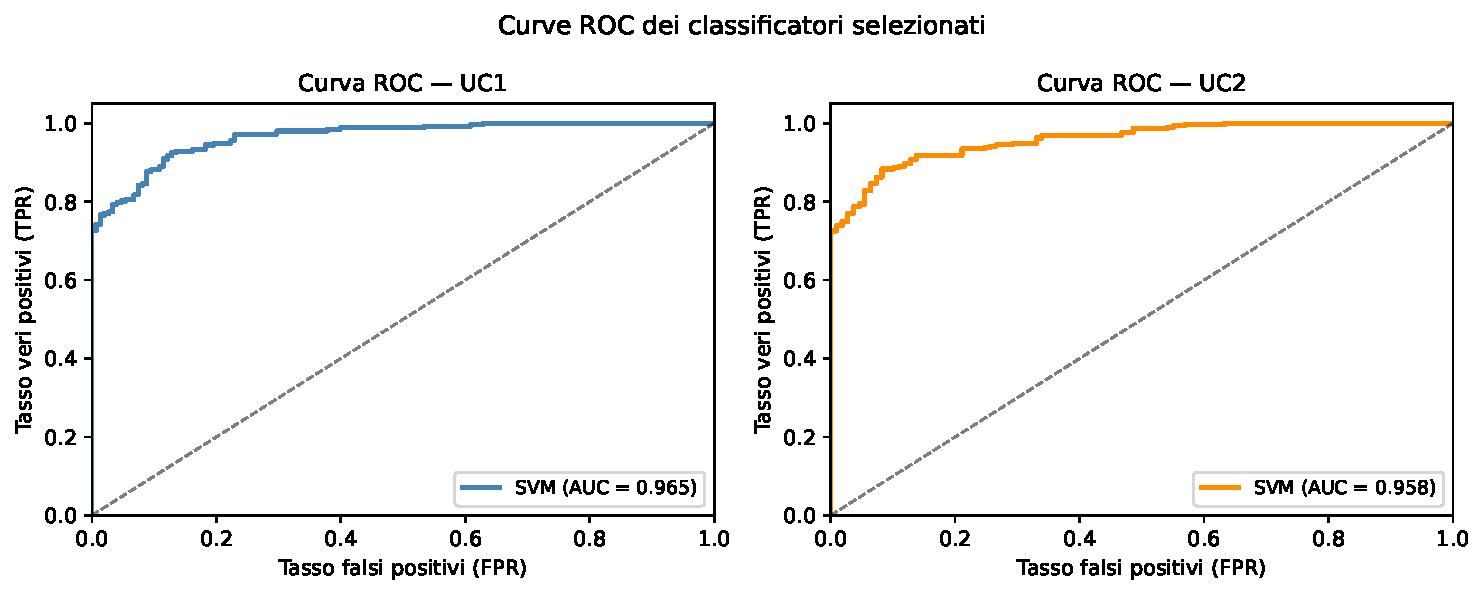
\includegraphics[width=0.85\textwidth]{fig_roc_curve.pdf}

\caption[Curve ROC dei classificatori TOP-1 selezionati]{Curve ROC
    sul test set indipendente dei due classificatori \acs{SVM} selezionati
    mediante validation. Le aree sono $0.965$ (UC1) e $0.958$ (UC2); la
    diagonale rappresenta un classificatore casuale.}\label{fig:roc_curve}
\end{figure}

% -----------------------------------------------
\subsection[Audit delle etichette TOP-1 e TOP-16]{Audit delle Etichette: TOP-1 e TOP-16 Sono Problemi Diversi}
\label{sec:audit_etichette}

La campagna calcola entrambe le etichette sullo \emph{stesso}
istogramma. L'esito è
riassunto nella Tabella~\ref{tab:audit_etichette}.

\begin{table}[H]
\centering

\begin{tabular}{lrr}
\toprule
\textbf{Regola} & \textbf{UC1: positivi/negativi} &
\textbf{UC2: positivi/negativi} \\
\midrule
TOP-1  & $1\,262/738$ & $1\,453/547$ \\
\addlinespace[0.3em]
TOP-16 & $2\,000/0$   & $2\,000/0$ \\
\bottomrule
\end{tabular}
\caption[Audit delle etichette TOP-1 e TOP-16]{Bilanciamento delle due
regole sul dataset completo. TOP-16 è a classe unica e non consente un
addestramento discriminante.}\label{tab:audit_etichette}

\end{table}

Il runner non forza un modello sul dataset TOP-16: registra
esplicitamente \texttt{single-class-dataset} e interrompe
l'addestramento per quella regola. M2 usa perciò soltanto i modelli TOP-1
e conserva nel payload \texttt{label\_top\_k=1}. Questo controllo evita
di attribuire capacità predittiva a un classificatore costante.

Una diagnostica separata su 60 esecuzioni nominali UC1 chiarisce la
struttura della classe TOP-1. La moda è $y=0$ in $30/60$ casi e conduce
ai fattori negli altri $30/60$; i primi quattro candidati contengono
invece almeno un esito utile in $60/60$ casi. La Tabella
\ref{tab:struttura_negativi} riporta la distribuzione della moda.

\begin{table}[H]
\centering

\begin{tabular}{lrr}
\toprule
\textbf{Valore della moda} & \textbf{Occorrenze} & \textbf{Frazione} \\
\midrule
$0$   & 30 & $50.0\%$ \\
\addlinespace[0.3em]
$64$  &  5 & $8.3\%$ \\
\addlinespace[0.3em]
$128$ & 15 & $25.0\%$ \\
\addlinespace[0.3em]
$192$ & 10 & $16.7\%$ \\
\bottomrule
\end{tabular}
\caption[Distribuzione della moda su UC1]{Distribuzione della misura più
frequente su 60 istogrammi nominali indipendenti.}\label{tab:struttura_negativi}

\end{table}

L'esito $y=0$ rappresenta la fase nulla e non fornisce il periodo, ma
non implica che l'istogramma sia privo di segnale. Nel campione
rappresentativo della Figura~\ref{fig:audit_istogramma_negativo}, la
moda $y=0$ raccoglie 176 conteggi, mentre $y=64$, $192$ e $128$ ne
raccolgono rispettivamente 160, 141 e 131: tutti e tre conducono ai
fattori. La massa complessiva sui quattro picchi è $0.594$.

\begin{figure}[H]
    \centering
    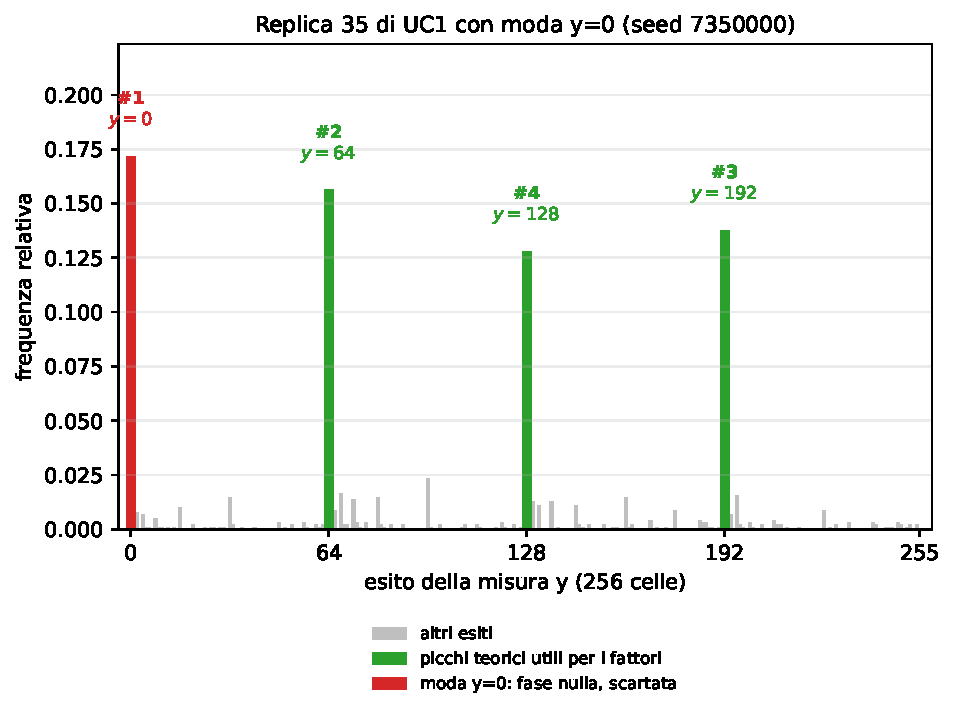
\includegraphics[width=0.86\textwidth]{audit_istogramma_negativo.pdf}

\caption[Istogramma TOP-1 negativo ma recuperabile con TOP-4]{Esempio
    nominale UC1 in cui TOP-1 fallisce perché la moda è $y=0$, mentre i
    successivi tre picchi conducono ai fattori. Il classificatore TOP-1
    apprende quindi una regola sul candidato dominante, non una misura
    generale della presenza di segnale quantistico.}\label{fig:audit_istogramma_negativo}
\end{figure}

\subsubsection{Perché TOP-16 Produce una Classe Quasi Sempre Positiva}
\label{subsec:soglia_classe_negativa}

Per $N=15$, $a=7$ e otto bit di controllo, 63 dei 256 esiti conducono ai
fattori tramite la procedura di frazioni continue adottata. Anche per un
istogramma uniforme, la probabilità che nessuno dei primi $K$ candidati
sia utile è quindi
\begin{equation}
    P_{\mathrm{neg}}(K)=
    \frac{\binom{256-63}{K}}{\binom{256}{K}}.
    \label{eq:tetto_negativi}
\end{equation}
Per $K=16$ essa vale soltanto $0.9275\%$: la regola assegna dunque
un'etichetta positiva a oltre il $99\%$ degli istogrammi uniformi per
puro effetto combinatorio. Il risultato $2\,000/0$ osservato nei due
dataset è coerente con questo limite e non autorizza a concludere che il
segnale sia perfetto.


\begin{figure}[H]
    \centering
    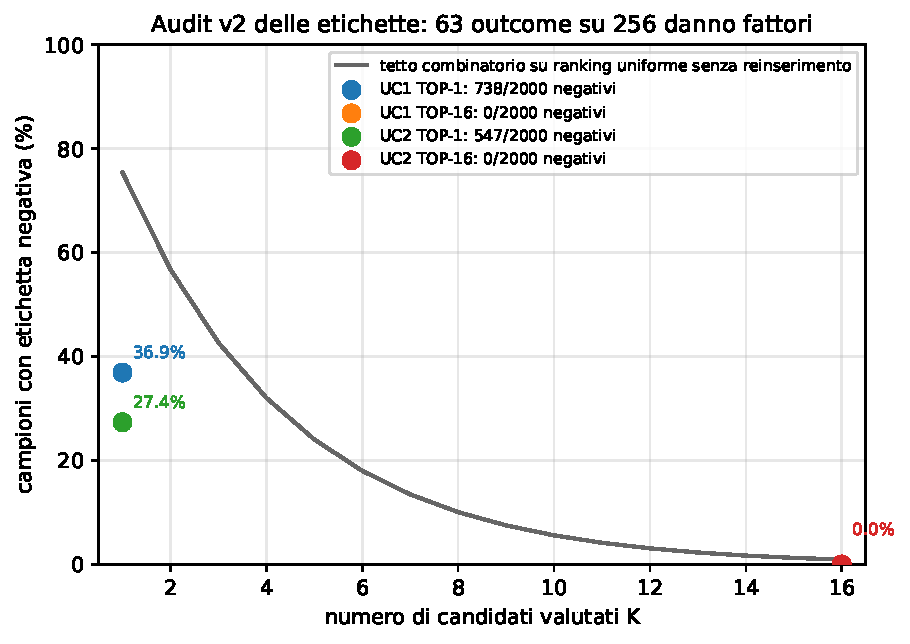
\includegraphics[width=0.78\textwidth]{tetto_classe_negativa.pdf}

\caption[Tetto combinatorio alla classe negativa]{Decadimento di
    $P_{\mathrm{neg}}(K)$ al crescere del numero di candidati. La figura
    è rigenerata dai dati schema~2 e rende visibile perché TOP-16 non
    definisce un problema di classificazione bilanciato su questa
    istanza.}\label{fig:tetto_classe_negativa}
\end{figure}

Il verdetto ha un perimetro preciso: non mostra che l'apprendimento
automatico sia inutile in generale, ma che un filtro a valle addestrato
su TOP-1 replica una decisione già superata da TOP-4, mentre la regola
TOP-16 è quasi sempre positiva per costruzione. Questo motiva lo
spostamento dell'apprendimento dalla distribuzione finale alla sindrome
di errore nelle sezioni del Capitolo~\ref{chap:risultati} dedicate alla \ac{QEC}.

\end{onehalfspace}

\chapter{Fase 2: la campagna QEC nel dettaglio}
\captionsetup[figure]{font=small,labelfont=bf}
\label{app:fase2}

\section{Laboratori preliminari QEC: codici a ripetizione e di Steane}
\label{app:laboratori_qec}
\begin{onehalfspace}

Questa sezione riporta i protocolli dei laboratori sul codice a ripetizione e
sul codice di Steane (Sezioni~\ref{sec:repetition} e~\ref{sec:steane}): gli
strumenti concettuali, le lookup table e le assunzioni necessarie a verificarne
i risultati.

\subsection{Dalla ridondanza alla codifica per stabilizzatori}
\label{app:qec_richiami}

L'idea classica di trasmettere tre copie di un bit e decidere a maggioranza
non si trasferisce direttamente al caso quantistico. Il teorema di
no-cloning~\cite{wootters1982} impedisce di copiare uno stato ignoto e la
misura diretta distruggerebbe la sovrapposizione da proteggere. La
\ac{QEC} codifica invece l'informazione di un qubit logico nelle
correlazioni di più qubit fisici~\cite{shorcorrection1995,steane1996,roffe2019}.
Operatori ausiliari rivelano quale classe di errore si è verificata senza
rivelare i coefficienti dello stato logico.

Il ciclo generale comprende: (i) codifica di $\ket{\psi_L}$; (ii) azione
del rumore; (iii) estrazione della sindrome mediante ancille; (iv)
decodifica classica; (v) correzione fisica o aggiornamento del \emph{Pauli
frame}. Uno stabilizzatore $S$ lascia invariati gli stati del codice,
$S\ket{\psi_L}=\ket{\psi_L}$: un esito $-1$ segnala l'uscita dal
sottospazio valido senza distinguere gli stati logici che lo compongono.

Un codice $[[n,k,d]]$ usa $n$ qubit fisici per $k$ qubit logici e ha
distanza $d$, pari al peso minimo di un errore logico non rilevato. Può
correggere
\begin{equation}
 t=\left\lfloor\frac{d-1}{2}\right\rfloor
 \label{eq:distanza_t}
\end{equation}
errori arbitrari. Il teorema della soglia garantisce in linea di principio
un regime in cui l'aumento della distanza riduce l'errore
logico~\cite{aharonov1997fault}; la sua osservazione quantitativa è oggetto
della Sezione~\ref{sec:surface_risultati}.

\begin{table}[H]

\centering
\small
\begin{tabularx}{\textwidth}{@{}>{\raggedright\arraybackslash}p{2.0cm}>{\raggedright\arraybackslash}p{1.9cm}XXX@{}}
\toprule
\textbf{Codice} & \textbf{Parametri} & \textbf{Corregge} & \textbf{Pro / Contro} & \textbf{Uso nella tesi} \\
\midrule
Repetition (bit-flip) & $[[3,1,1]]$ su X & solo bit-flip & semplice / non corregge phase-flip & primo laboratorio \\
\addlinespace[0.3em]
Repetition (phase-flip) & 3 qubit, base H & solo phase-flip & mostra dualità X/Z / parziale & controllo duale \\
\addlinespace[0.3em]
Shor code & $[[9,1,3]]$ & errore arbitrario singolo & storico, intuitivo / più pesante & richiamo didattico~\cite{shorcorrection1995} \\
\addlinespace[0.3em]
Steane code & $[[7,1,3]]$ & errore arbitrario singolo & \ac{CSS}, compatto / distanza bassa & secondo laboratorio~\cite{steane1996} \\
\addlinespace[0.3em]
Five-qubit & $[[5,1,3]]$ & errore arbitrario singolo & minimo / non \ac{CSS} & confronto teorico \\
\addlinespace[0.3em]
Surface code & $d^2$ dati $+O(d^2)$ ancille & errori locali su griglia 2D & scalabile / overhead elevato & campagna principale~\cite{fowler2012} \\
\bottomrule
\end{tabularx}
\caption[Confronto tra codici correttori quantistici]{Confronto esteso e
progressione metodologica: repetition per introdurre la sindrome, Steane
per un errore arbitrario, surface code per soglia e scalabilità.}\label{tab:confronto_codici}

\end{table}

\subsection{Protocollo completo del codice a ripetizione}
\label{app:qec_repetition}

Il codice contro errori X codifica $\ket{0_L}=\ket{000}$ e
$\ket{1_L}=\ket{111}$: lo stato
$\alpha\ket{0}+\beta\ket{1}$ diventa
$\alpha\ket{000}+\beta\ket{111}$, uno stato entangled e non tre copie.
Gli stabilizzatori $Z_1Z_2$ e $Z_2Z_3$ misurano la parità tramite due
ancille. Il duale nella base di Hadamard usa $X_1X_2$ e $X_2X_3$ e
protegge dagli errori Z; la concatenazione delle due protezioni conduce
al codice di Shor a nove qubit.

Il primo controllo inietta deterministicamente un errore su ciascun qubit
dato e verifica che la sindrome identifichi la posizione senza misurare
l'informazione logica.

\begin{table}[H]

\centering
\begin{tabular}{lccc}
\toprule
\textbf{Errore iniettato} & \textbf{Sindrome $(a_0,a_1)$} & \textbf{Qubit dedotto} & \textbf{Esito} \\
\midrule
nessuno & $(0,0)$ & --- & $\surd$ \\
\addlinespace[0.3em]
su $q_0$ & $(1,0)$ & $q_0$ & $\surd$ \\
\addlinespace[0.3em]
su $q_1$ & $(1,1)$ & $q_1$ & $\surd$ \\
\addlinespace[0.3em]
su $q_2$ & $(0,1)$ & $q_2$ & $\surd$ \\
\bottomrule
\end{tabular}
\caption[Verifica della sindrome del codice a ripetizione]{Lookup table
verificata per il codice bit-flip e per il duale phase-flip. L'ancilla
$a_0$ misura la parità di $\{0,1\}$ e $a_1$ quella di $\{1,2\}$. La
coincidenza cifra per cifra a parità di seed verifica l'implementazione
della dualità, non costituisce una conferma indipendente del fatto
algebrico.}\label{tab:sindrome_repetition}

\end{table}

Il secondo controllo prepara lo stato logico, applica a ciascun qubit un
errore indipendente con probabilità $p$, estrae la sindrome, corregge e
decodifica. I $20\,000$ campioni per punto (seed 42) producono la curva
discussa nella Sezione~\ref{sec:repetition}. Un errore Z resta
invisibile al codice bit-flip, e viceversa per il duale: è il limite che
motiva il passaggio allo Steane.

\subsection{Struttura e protocollo completo del codice di Steane}
\label{app:qec_steane}

Lo Steane~\cite{steane1996} è un codice \ac{CSS} derivato dal codice di
Hamming $[7,4,3]$: codifica un qubit in sette, ha distanza 3 e corregge
un errore X, Z o Y su un singolo qubit.

\begin{table}[H]

\centering
\begin{tabular}{lcl}
\toprule
\textbf{Parametro} & \textbf{Valore} & \textbf{Significato} \\
\midrule
$n$ & 7 & qubit fisici \\
\addlinespace[0.3em]
$k$ & 1 & qubit logici \\
\addlinespace[0.3em]
$d$ & 3 & distanza \\
\addlinespace[0.3em]
$t$ & 1 & errori arbitrari correggibili (Eq.~\ref{eq:distanza_t}) \\
\addlinespace[0.3em]
Tipo & \ac{CSS} & sindromi X e Z separate \\
\bottomrule
\end{tabular}
\caption[Parametri del codice di Steane]{Parametri del codice di Steane $[[7,1,3]]$.}\label{tab:steane_parametri}

\end{table}

Nella convenzione adottata i generatori sono
\begin{equation}
\begin{aligned}
\text{tipo X:}\quad & IIIXXXX,\quad IXXIIXX,\quad XIXIXIX,\\
\text{tipo Z:}\quad & IIIZZZZ,\quad IZZIIZZ,\quad ZIZIZIZ.
\end{aligned}
\label{eq:steane_stabilizzatori}
\end{equation}
Gli stabilizzatori Z rilevano gli errori X, quelli X rilevano gli errori
Z e un errore Y accende entrambe le famiglie. I tre bit di sindrome,
letti come numero binario, indicano la posizione del qubit colpito.

Il protocollo comprende: preparazione di $\ket{0_L}$ o $\ket{+_L}$;
iniezione manuale di X, Z e Y su ciascuno dei sette qubit; misura della
sindrome; costruzione della lookup table; stima della correzione al
variare di $p$; distinzione fra errori sui dati e sulle ancille. La
preparazione di $\ket{0_L}$ usa tre qubit seme in sovrapposizione e una
rete CNOT; i sei stabilizzatori restituiscono $000000$ su tutti i
$2\,000$ campioni, verificando l'appartenenza al code space.

\begin{table}[H]

\centering
\begin{tabular}{cccc}
\toprule
\textbf{Qubit} & \textbf{Sindrome} & \textbf{Valore} & \textbf{Correzione} \\
\midrule
$q_0$ & $001$ & 1 & applica $X$ (o $Z$) su $q_0$ \\
\addlinespace[0.3em]
$q_1$ & $010$ & 2 & applica su $q_1$ \\
\addlinespace[0.3em]
$q_2$ & $011$ & 3 & applica su $q_2$ \\
\addlinespace[0.3em]
$q_3$ & $100$ & 4 & applica su $q_3$ \\
\addlinespace[0.3em]
$q_4$ & $101$ & 5 & applica su $q_4$ \\
\addlinespace[0.3em]
$q_5$ & $110$ & 6 & applica su $q_5$ \\
\addlinespace[0.3em]
$q_6$ & $111$ & 7 & applica su $q_6$ \\
\bottomrule
\end{tabular}
\caption[Syndrome table del codice di Steane]{Tabella
sindrome--qubit--correzione verificata per tutti i 21 casi: X, Z e Y su
ciascuno dei sette qubit.}\label{tab:steane_sindrome}

\end{table}

La simulazione Monte Carlo usa $200\,000$ campioni per punto (seed 42),
applica la correzione a peso minimo e verifica il residuo logico. La
versione implementata assume errori sui qubit dati e sindrome ideale:
l'estrazione non è fault-tolerant. Un guasto sulle ancille può corrompere
la sindrome e indurre una correzione errata; i cicli rumorosi e ripetuti
del surface code affrontano precisamente questo limite.

\end{onehalfspace}

% -----------------------------------------------

\section{Surface code: protocollo e controlli sul modello}
\label{app:surface_protocollo_generale}
\begin{onehalfspace}

Questa sezione approfondisce le Sezioni~\ref{sec:surface_concetto}--\ref{sec:oltre_pauli}
con il funzionamento del codice, la griglia sperimentale, le verifiche di
riproducibilità e il controllo sui canali non-Pauli.

\subsection{Surface code e decodifica MWPM}
\label{app:surface_teoria}

Il surface code~\cite{kitaev2003,fowler2012} dispone su una griglia
bidimensionale qubit dati e qubit di misura. Gli stabilizzatori sono locali
e un patch planare ruotato di distanza $d$ usa $d^2$ dati, oltre a un
numero dello stesso ordine di ancille. Le misure sono ripetute per più
round perché anche la sindrome è rumorosa; una variazione fra due cicli
costituisce un \emph{detection event}.

Nel bulk, una catena d'errore produce tipicamente detection events in
coppie; al bordo uno dei due estremi può terminare sul confine. Il
\ac{MWPM} associa gli eventi minimizzando un peso collegato alla
probabilità delle catene~\cite{pymatching2021}. Se errore reale e
correzione differiscono per un ciclo che attraversa il patch, si verifica
un errore logico silenzioso: la sua frequenza è $p_L$.

La stima richiede milioni di circuiti con centinaia di qubit, ma i memory
experiment sono circuiti stabilizer. Stim~\cite{stim2021} sfrutta il
teorema di Gottesman--Knill per campionare detection events; PyMatching
costruisce il grafo dal \ac{DEM} e decodifica. Il Listato~\ref{lst:stim_pymatching}
nella Sezione~\ref{app:codice} documenta l'implementazione. Shor non è un
circuito stabilizer: per questo i tassi del memory experiment non sono
trasferiti direttamente alla successiva analisi di sensibilità.

\subsection{Griglia sperimentale e riproducibilità}
\label{app:surface_protocollo}

\begin{table}[H]

\centering
\begin{tabularx}{\textwidth}{llX}
\toprule
\textbf{Variabile} & \textbf{Valori} & \textbf{Osservazione attesa} \\
\midrule
distanza $d$ & 3, 5, 7, 9 & $p_L$ diminuisce con $d$ sotto soglia \\
\addlinespace[0.3em]
rounds & $d$ e $2d$ & cicli di memoria quantistica \\
\addlinespace[0.3em]
$p$ fisico & $10^{-4}$ \dots $2\times10^{-2}$ & curva $p$--$p_L$ \\
\addlinespace[0.3em]
shot & $\geq10^4$ per punto & intervalli di confidenza stabili \\
\addlinespace[0.3em]
base & memory X e memory Z & controllo delle due protezioni \\
\bottomrule
\end{tabularx}
\caption[Disegno sperimentale surface code]{Griglia prescritta. La
campagna eseguita copre le quattro distanze, entrambe le basi,
$\mathrm{rounds}=d$ e $p\in[2\times10^{-3},10^{-2}]$; lo scaling a
$2d$ resta un'estensione.}\label{tab:surface_esperimento}

\end{table}

Il modello è circuit-level: depolarizzazione dopo ogni Clifford e flip di
reset e misura con probabilità $p$. Il campione è dimensionato punto per
punto per raccogliere circa duecento eventi logici, da $2\times10^5$ a
$4\times10^7$ shot. Una prima passata da $2\times10^5$ stima l'ordine di
grandezza di $p_L$; la seconda fissa la numerosità. A $d=9$ e
$p=2\times10^{-3}$ una numerosità fissa darebbe due soli eventi e il
$70\%$ di incertezza relativa, mentre il campionamento adattivo la porta
al $3.5\%$. Seed e numerosità sono registrati per ogni punto. Una
ripetizione indipendente ha riprodotto tutte le stime entro l'errore
statistico e le stesse soglie.

\subsection{Errori coerenti, leakage e controllo full-state}
\label{app:surface_non_pauli}

Stim rappresenta gate Clifford ed errori Pauli casuali. L'hardware può
però produrre sovrarotazioni coerenti, leakage verso $\ket{2}$ e
correlazioni temporali; una simulazione solo Clifford--Pauli può quindi
essere ottimistica~\cite{plaquette2026}. In una sovrarotazione
$U=e^{-i\varepsilon H}$ le ampiezze si sommano coerentemente, mentre un
errore stocastico accumula probabilità.

Il divario è illustrato da un qubit soggetto a $N$ operazioni con
$p=10^{-2}$, modellate come X stocastico oppure come
$R_X(\theta)$ con $\sin^2(\theta/2)=p$. Le probabilità esatte sono
$[1-(1-2p)^N]/2$ e $\sin^2(N\theta/2)$; nel tratto iniziale crescono
come $Np$ e $N^2p$. A $N=8$ il secondo errore è circa sette volte il
primo per i parametri scelti.

\begin{figure}[H]
\centering
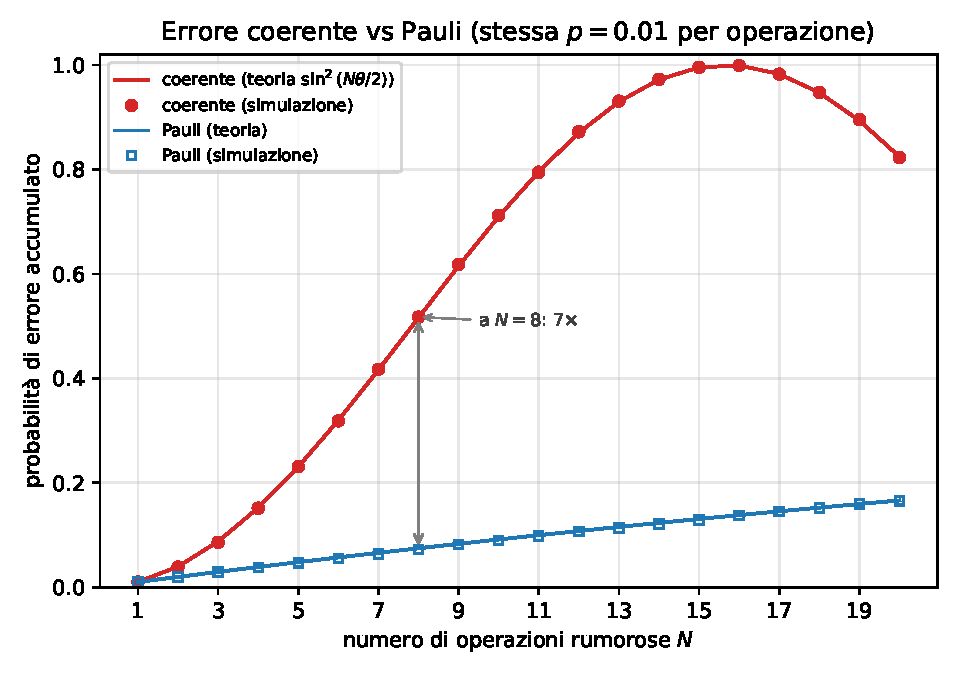
\includegraphics[width=0.72\textwidth,height=0.30\textheight,keepaspectratio]{qec_coherent.pdf}

\caption[Errore coerente vs errore di Pauli]{Accumulo su un qubit a
parità di probabilità marginale per operazione. La simulazione full-state
(marcatori) coincide con le espressioni teoriche; il fattore osservato non
è universale.}\label{fig:qec_coherent}
\end{figure}

Lo studio di riferimento riporta, in altri regimi, errori logici
$1.7\%$ contro $23.5\%$ in presenza di leakage e $18.1\%$ contro
$38.7\%$ con errori coerenti; per un surface code a distanza 9 il divario
può raggiungere un fattore 25--56 e spostare la soglia di circa il
$20\%$~\cite{plaquette2026}. Questi valori non sono trasferiti alla
campagna della tesi: motivano un approccio channel-first, nel quale il
canale fisico è definito una volta e approssimato solo dopo aver stabilito
quale informazione preservare.

Il controllo interno usa un codice a distanza 3 simulato full-state per
quattro cicli, confrontando X di Pauli e $R_X$ coerente a pari
probabilità marginale. A $p=3\times10^{-2}$ il canale coerente produce
meno flip grezzi ($0.237$ contro $0.262$) ma un errore MWPM leggermente
maggiore ($0.0789$ contro $0.0767$, $+2.9\%$). Le misure ripetute
interrompono parte dell'accumulo coerente, senza equivalere a un twirling
Pauli completo.

Il decoder ibrido ottiene guadagni $1.019$, $1.036$, $1.041$ sotto Pauli
e $1.029$, $1.048$, $1.052$ sotto sovrarotazione, per
$p=1,2,3\times10^{-2}$. Lo scarto è circa una deviazione standard e non
è significativo. Il risultato esclude quindi la regola semplicistica
``non-Pauli implica vantaggio appreso'': ciò che il matching non
rappresenta è la non decomponibilità in archi, come nel crosstalk che
accende più di due detector. Le soglie del corpo restano baseline entro
il modello Pauli; leakage e canali più ricchi sono sviluppi futuri.

\end{onehalfspace}

% -----------------------------------------------

\section{La decodifica appresa: la campagna completa}
\label{app:decodifica}

Questa sezione completa le evidenze E1--E4 presentate nella
Sezione~\ref{sec:decodifica_appresa} con i controlli di scala, trasferibilità,
calibrazione e scelta della baseline, che rendono verificabili i limiti del
decoder ibrido.

\paragraph{Il limite: il vantaggio non sopravvive alla distanza 7.}
Il dato più importante della Tabella~\ref{tab:neural_ibrido} è però l'ultimo blocco, e va enunciato senza attenuazioni. A distanza 7 l'ibrido \textbf{non ribalta alcuno shot} in nessuna delle cinque configurazioni: la soglia scelta in validazione è ogni volta quella corrispondente a ``non ribaltare mai'', e il decoder ibrido coincide con il \ac{MWPM} cifra per cifra. Il guadagno svanisce, e la progressione lungo le tre distanze è inequivocabile: $18$--$21\%$ a $d=3$, $1$--$3\%$ a $d=5$, esattamente zero a $d=7$.

Due meccanismi possono spiegarlo, e vanno separati perché conducono a rimedi diversi. Il primo è la \textbf{scarsità di esempi}: l'evento da riconoscere è il fallimento del matching, la cui frequenza \emph{è} $p_L$, e $p_L$ decresce esponenzialmente con $d$. In assenza di crosstalk, a $d=7$ si hanno $p_L = 5.5\times10^{-4}$ e $8\times10^5$ shot, ossia $264$ esempi positivi nella partizione di addestramento, per un ingresso a $336$ dimensioni. Il secondo è la \textbf{capacità rappresentativa}: la rete densa impiegata tratta i detector come dimensioni indipendenti, e ciò che distingue le due classi di errore su un reticolo grande è una correlazione a lungo raggio fra detector distanti.

Un primo indizio viene dal semplice conteggio. La spiegazione per scarsità è esatta nella configurazione senza crosstalk, dove i fallimenti del matching sono effettivamente poche centinaia; ma nelle altre quattro configurazioni a $d=7$ la rete dispone da $1.8\times10^4$ a $2.2\times10^5$ esempi positivi --- fino a duecentomila --- e continua a non ribaltare alcuno shot. La spiegazione copre dunque una configurazione su cinque.

L'indizio non basta però a stabilire la causa, perché fra $d=5$ (che funziona) e $d=7$ (che non funziona) cambiano \emph{due} cose insieme: la distanza del codice e il numero di detector. L'esperimento E9 le separa, sfruttando il fatto che il numero di detector è il prodotto fra gli stabilizzatori per ciclo e il numero di cicli, e può quindi essere variato a distanza fissa. Ne risulta un incrocio $2\times2$ le cui celle diagonali distinguono le due ipotesi, riportato nella Tabella~\ref{tab:neural_esempi}.

\begin{table}[H]

\centering
\small
\begin{tabular}{ccc rc rc}
\toprule
& & & \multicolumn{2}{c}{$p_{ct} = 0.005$} & \multicolumn{2}{c}{$p_{ct} = 0.02$} \\
\cmidrule(lr){4-5}\cmidrule(lr){6-7}
$d$ & \textbf{cicli} & \textbf{detector} & \textbf{es.\ pos.} & \textbf{residuo} & \textbf{es.\ pos.} & \textbf{residuo} \\
\midrule
7 & \phantom{0}3 & \textbf{144} & \phantom{00}5\,933 & si astiene & \phantom{0}61\,900 & \textbf{interviene} \\
\addlinespace[0.3em]
7 & \phantom{0}7 & 336 & \phantom{0}17\,665 & si astiene & 139\,275 & si astiene \\
\addlinespace[0.3em]
5 & 14 & 336 & \phantom{0}48\,657 & si astiene & 188\,582 & si astiene \\
\addlinespace[0.3em]
5 & \phantom{0}5 & \textbf{120} & \phantom{0}17\,235 & \textbf{interviene} & \phantom{0}96\,167 & \textbf{interviene} \\
\bottomrule
\end{tabular}
\caption[Larghezza dell'ingresso contro distanza del codice]{Esperimento E9: incrocio fra distanza del codice e numero di detector, ottenuto variando il numero di cicli di estrazione della sindrome. ``Es.\ pos.'' è il numero di fallimenti del \ac{MWPM} disponibili all'addestramento su $4.8\times10^5$ shot; ``residuo'' indica se il criterio di validazione seleziona una soglia che ribalta almeno uno shot su diecimila. Le righe centrali sono le celle diagonali, quelle che distinguono le ipotesi: a distanza 5 con $336$ detector e $1.9\times10^5$ esempi il residuo si astiene, a distanza 7 con $144$ detector e tre volte meno esempi interviene. Il comportamento segue la colonna, non la riga.}\label{tab:neural_esempi}

\end{table}

L'esito è netto su entrambe le diagonali e va letto per colonne. A $336$ detector il residuo si astiene sempre, a qualunque distanza e con qualunque numerosità --- fino a $1.9\times10^5$ esempi positivi; a $120$ e $144$ detector interviene, anche a distanza 7 e anche con tre volte meno esempi. \textbf{L'ipotesi della distanza è confutata, quella della larghezza dell'ingresso è confermata.}

Una sfumatura completa l'enunciato e lo rende più preciso. A $144$ detector con soli $5\,933$ esempi positivi il residuo si astiene: la numerosità \emph{è} dunque un vincolo reale, al margine inferiore. Non è però il vincolo che opera nell'esperimento E4 a distanza 7, dove gli esempi erano $1.4\times10^5$ e la rete si asteneva comunque. La formulazione corretta è che disporre di abbastanza esempi è \emph{necessario ma non sufficiente}, e che a parità di numerosità sufficiente è la larghezza dell'ingresso a decidere.

\paragraph{Che cosa significhi esattamente ``si astiene'' (E12).}
Il verbo va però disinnescato, perché astenersi è l'esito di una \emph{selezione}: fra le soglie candidate figura quella corrispondente a ``non ribaltare mai'', e che vinca in validazione significa che agire non conviene, non che non vi sia nulla da vedere. La distinzione non è oziosa, perché le due letture conducono a rimedi opposti --- un'architettura diversa nella prima, una regola di decisione diversa nella seconda. L'esperimento E12 la risolve misurando l'\ac{AUC} del residuo, che quantifica quanto la rete \emph{ordini} i fallimenti del matching indipendentemente da qualunque soglia, e affiancando alla soglia scelta onestamente in validazione una soglia \emph{oracolo}, la migliore sul test set stesso: inutilizzabile in pratica, ma limite superiore assoluto di ciò che qualunque regola di decisione potrebbe ottenere.

\begin{table}[H]

\centering
\small
\begin{tabular}{rcc cc c}
\toprule
\textbf{detector} & $d$ & \textbf{cicli} & \textbf{AUC} & \textbf{guadagno onesto} & \textbf{guadagno oracolo} \\
\midrule
\phantom{0}24 & 3 & \phantom{0}3 & 0.912 & 1.2215 & 1.2233 \\
\addlinespace[0.3em]
120 & 5 & \phantom{0}5 & 0.769 & 1.0206 & 1.0215 \\
\addlinespace[0.3em]
144 & 7 & \phantom{0}3 & 0.788 & 1.0066 & 1.0066 \\
\addlinespace[0.3em]
336 & 7 & \phantom{0}7 & 0.621 & 1.0000 & 1.0000 \\
\addlinespace[0.3em]
336 & 5 & 14 & 0.573 & 1.0000 & 1.0003 \\
\bottomrule
\end{tabular}
\caption[Discriminazione e guadagno al crescere della larghezza dell'ingresso]{Esperimento E12 a $p_{ct} = 2\times10^{-2}$. L'\ac{AUC} è calcolata sul test set con bersaglio ``il \ac{MWPM} ha sbagliato''. Il guadagno oracolo usa la soglia migliore sul test set stesso e non è quindi realizzabile: serve unicamente a stabilire quanto del divario sia imputabile alla calibrazione. Ai livelli di crosstalk più bassi il quadro è il medesimo, con \ac{AUC} sistematicamente più alte ($0.958$ a $24$ detector, $0.771$ a $336$).}\label{tab:neural_auc}

\end{table}

Il risultato smentisce entrambe le letture immediate. \textbf{La rete non è cieca}: a $336$ detector l'\ac{AUC} vale $0.57$--$0.77$, ben sopra il caso, e la rete ordina dunque i fallimenti del matching assai meglio del lancio di una moneta. \textbf{Ma non si tratta neppure di calibrazione}: il guadagno oracolo è $1.0000$, sicché nemmeno scegliendo la soglia sui dati di valutazione si otterrebbe alcunché.

La spiegazione sta nella forma stessa della correzione residuale, ed è quantitativa. Il ribaltamento è \emph{simmetrico}: ribaltare uno shot che il matching aveva risolto costa esattamente quanto ribaltarne uno che aveva sbagliato rende. Perché l'operazione sia in attivo occorre dunque che fra gli shot ribaltati la \textbf{precisione superi il cinquanta per cento} --- una soglia netta, non un ottimo graduale. L'\ac{AUC} necessaria a raggiungerla dipende dal tasso di base: a $24$ detector e crosstalk $5\times10^{-3}$ il tasso di base è del $3.1\%$ e un'\ac{AUC} di $0.958$ concentra i fallimenti abbastanza da superare la soglia, con un guadagno del $19\%$; a $336$ detector, a parità di tasso di base, un'\ac{AUC} di $0.771$ richiederebbe un fattore di concentrazione quattordici volte superiore a quello che produce. Nessuna soglia porta la precisione sopra il cinquanta per cento, e il guadagno è allora \emph{esattamente} $1.000$ --- non approssimativamente: è questa discontinuità a spiegare il salto brusco osservato lungo la Tabella~\ref{tab:neural_esempi}.

Ne discendono due conseguenze. La prima è che \textbf{l'astensione del criterio di validazione è corretta e non conservativa}: la soglia oracolo conferma che intervenire non converrebbe, e il metodo si comporta esattamente come dichiarato al momento della sua costruzione. La seconda riguarda il rimedio, e ne precisa il criterio di successo: un'architettura convoluzionale o a grafo è utile se e soltanto se innalza l'\ac{AUC} quanto basta a riportare la precisione sopra la soglia del cinquanta per cento, che è una condizione verificabile in anticipo su una rete addestrata --- assai più informativa dell'osservazione che il modello ``non regge''.

Questa è la delimitazione del risultato di M10, e conviene formularla in positivo. Il guadagno del decoder ibrido è supportato da un valore nominale del test di McNemar praticamente nullo a $d=3$ (inferiore a $10^{-300}$), ma vive nel regime in cui la sindrome è stretta abbastanza da lasciare alla rete densa una discriminazione sufficiente a superare la soglia di precisione. Il valore $p$ quantifica l'incompatibilità con l'ipotesi nulla nel modello del test, non la dimensione pratica dell'effetto, riportata separatamente tramite la riduzione di $p_L$. Poiché è proprio la crescita della distanza a costituire la strategia della correzione d'errore scalabile, il metodo così com'è non accompagna il codice nel regime che conta. Il rimedio indicato dalla diagnosi non è raccogliere più campioni --- ne bastavano già --- ma innalzare la discriminazione a parità di larghezza dell'ingresso, il che significa cambiare architettura: una rete convoluzionale o a grafo, che condivida i pesi fra regioni equivalenti del reticolo anziché trattare i $336$ detector come dimensioni indipendenti, sfrutta la simmetria traslazionale del problema e rappresenta con pochi parametri le correlazioni locali che la rete densa deve stimare una per una. È l'estensione naturale, e la si indica fra gli sviluppi futuri (Capitolo~\ref{chap:sviluppi}).

\subsection[E6 - modello del decoder errato?]{E6 - e se il modello del decoder fosse semplicemente sbagliato?}
\label{subsec:neural_miscalibrato}

Gli esperimenti fin qui condotti concedono al \ac{MWPM} un vantaggio che l'hardware non offre: il detector error model che ne pesa gli archi è generato da Stim \emph{dal circuito stesso}, ed è quindi una descrizione esatta del rumore. Un decoder in produzione lavora invece su un modello ricavato dalla calibrazione del dispositivo --- misurata a intervalli, soggetta a deriva, inevitabilmente diversa dal rumore del momento. Se il vantaggio del modello appreso nascesse da questa discrepanza, sarebbe un vantaggio molto più generale di quello osservato con il crosstalk, perché la mis-calibrazione è la condizione ordinaria di ogni \ac{QPU}.

L'esperimento la isola: il circuito viene campionato con il rumore reale, mentre il matching è costruito su un modello in cui l'errore di \emph{misura} è sbagliato di un fattore $(1+\delta)$ e quello di gate resta corretto.

\begin{table}[H]

\centering
\footnotesize
\setlength{\tabcolsep}{4pt}
\begin{tabular}{crccccc}
\toprule
$d$ & $\delta$ & \textbf{MWPM esatto} & \textbf{MWPM sbagliato} & \textbf{costo} & \textbf{rete} & \textbf{rete/MWPM} \\
\midrule
\multirow{6}{*}{3} & $-80\%$  & 0.00407 & 0.00415 & 1.018 & 0.00525 & 0.79 \\
\addlinespace[0.3em]
                   & $-50\%$  & 0.00435 & 0.00435 & 1.000 & 0.00493 & 0.88 \\
\addlinespace[0.3em]
                   & $0$      & 0.00427 & 0.00427 & 1.000 & 0.00558 & 0.77 \\
\addlinespace[0.3em]
                   & $+100\%$ & 0.00387 & 0.00382 & 0.987 & 0.00443 & 0.86 \\
\addlinespace[0.3em]
                   & $+300\%$ & 0.00388 & 0.00362 & 0.931 & 0.00429 & 0.84 \\
\addlinespace[0.3em]
                   & $+900\%$ & 0.00385 & 0.00392 & 1.017 & 0.00463 & 0.85 \\
\midrule
\multirow{6}{*}{5} & $-80\%$  & 0.00147 & 0.00153 & 1.034 & 0.02982 & 0.05 \\
\addlinespace[0.3em]
                   & $-50\%$  & 0.00172 & 0.00173 & 1.010 & 0.02855 & 0.06 \\
\addlinespace[0.3em]
                   & $0$      & 0.00163 & 0.00163 & 1.000 & 0.02784 & 0.06 \\
\addlinespace[0.3em]
                   & $+100\%$ & 0.00174 & 0.00175 & 1.005 & 0.02774 & 0.06 \\
\addlinespace[0.3em]
                   & $+300\%$ & 0.00169 & 0.00167 & 0.985 & 0.02888 & 0.06 \\
\addlinespace[0.3em]
                   & $+900\%$ & 0.00159 & 0.00191 & \textbf{1.199} & 0.03052 & 0.06 \\
\bottomrule
\end{tabular}
\caption[Effetto di un modello di rumore mis-calibrato sul MWPM]{Errore logico del \ac{MWPM} quando il modello che ne pesa gli archi attribuisce all'errore di misura il valore $p\,(1+\delta)$ anziché quello vero. La colonna ``costo'' è il rapporto fra l'errore logico con modello sbagliato e quello con modello esatto; ``rete/MWPM'' confronta il decoder appreso con il matching mis-calibrato --- valori inferiori a $1$ indicano che la rete è peggiore. Errore fisico reale $p = 3\times10^{-3}$, $4\times10^{5}$ campioni per configurazione.}\label{tab:neural_miscalibrato}

\end{table}

\begin{samepage}
\paragraph{Perché la perturbazione dev'essere sbilanciata.} Un primo tentativo scalava tutte le probabilità di errore dello stesso fattore, e non produceva alcun effetto misurabile: il costo rilevato era $1.000$, $1.004$ e $1.000$ per $\delta$ pari a $0$, $+100\%$ e $-50\%$. La ragione è istruttiva e merita di essere esplicitata, perché delimita ciò che una calibrazione errata può e non può fare. Il \ac{MWPM} minimizza il peso totale del matching, e il peso di un arco vale $\log\frac{1-p_e}{p_e} \approx -\log p_e$ per $p_e$ piccolo: moltiplicare tutte le $p_e$ per una costante trasla \emph{tutti} i pesi della stessa quantità, e un matching di peso minimo è invariante rispetto a una traslazione uniforme. Ciò che rende il matching vulnerabile non è dunque sbagliare la \emph{scala} del rumore, ma il suo \emph{bilanciamento}: il rapporto fra archi temporali, che rappresentano errori di misura, e archi spaziali, che rappresentano errori sui dati. È questo rapporto che l'esperimento perturba.
\end{samepage}



L'esito è netto in entrambe le direzioni. Il \ac{MWPM} si rivela \textbf{notevolmente robusto}: sbagliando l'errore di misura di un fattore cinque in difetto o dieci in eccesso, l'errore logico cambia tipicamente dell'$1$--$3\%$, e in due configurazioni \emph{migliora} leggermente. L'unico caso in cui la mis-calibrazione morde davvero è $d=5$ con $\delta = +900\%$, dove il costo sale al $20\%$: sovrastimare di un ordine di grandezza l'errore di misura induce il matching a preferire spiegazioni temporali degli eventi rilevati anche quando la spiegazione corretta è spaziale. Ma occorre appunto un errore di calibrazione di un ordine di grandezza perché l'effetto sia visibile.

La rete, dal canto suo, \textbf{non batte il matching in nessuna delle dodici configurazioni}, neppure quelle in cui esso lavora sul modello sbagliato. A $d=3$ resta indietro del $15$--$25\%$; a $d=5$ è peggiore di un fattore venti, in coerenza con il crollo osservato nell'esperimento precedente.

\paragraph{Che cosa questo precisa del criterio.}
Il risultato è negativo, ma corregge un'imprecisione nel modo in cui il criterio della tesi era stato finora formulato. Si era detto che il modello appreso produce valore dove il metodo analitico è ``cieco'' rispetto a una parte dell'informazione; questo esperimento mostra che la cecità rilevante non è quella dei \emph{parametri} ma quella della \emph{struttura}. Un modello con i parametri sbagliati continua a rappresentare le stesse classi di errore, e il matching che ne deriva resta quasi ottimale perché la geometria del problema --- quali eventi rilevati siano plausibilmente connessi --- non cambia. Un modello che non contempla affatto una classe di errore, come il crosstalk fra qubit di dato adiacenti dell'esperimento E2, sbaglia invece la geometria stessa, e lì il margine esiste. La formulazione corretta del criterio è dunque: \emph{l'apprendimento paga quando la classe di errore non è rappresentabile nella struttura del decoder, non quando è rappresentata con parametri imprecisi}.

Ne discende anche un'indicazione pratica, da leggere entro il perimetro dell'esperimento: quando a essere sbagliato è soltanto l'errore di misura attribuito al decoder, una calibrazione più accurata entro un ordine di grandezza non produce guadagni apprezzabili sulla decodifica. La conclusione non si estende ad altre forme di mis-calibrazione, come errori sbagliati in modo diverso da qubit a qubit o derive temporali.

\subsection[E7 - confronto con un decoder analitico migliore]{E7 - e se si scegliesse semplicemente un decoder analitico migliore?}
\label{subsec:neural_bposd}

Resta l'obiezione più severa che si possa muovere a tutto l'impianto della sezione. Il \ac{MWPM} è lo standard di fatto, ma non è il miglior decoder analitico disponibile: esso richiede che ogni meccanismo di errore sia decomponibile in archi di un grafo, e il crosstalk fra qubit di dato adiacenti viola precisamente questa ipotesi. Un decoder che non la richieda --- \textbf{BP+OSD}, ossia \textit{belief propagation} seguita da \textit{ordered statistics decoding}, che opera direttamente sulla matrice di parità del detector error model \cite{panteleev2021, roffe2020} --- potrebbe catturare da solo il margine attribuito all'apprendimento. Se così fosse, il risultato di E4 non misurerebbe il valore di un modello appreso ma il costo di una scelta subottimale del decoder di riferimento.

Il confronto è condotto sugli stessi circuiti e con la stessa mis-informazione: entrambi i decoder analitici ricevono il \ac{DEM} \emph{nominale}, privo di crosstalk, che è quanto un decoder reale avrebbe a disposizione. La significatività è valutata con il test di McNemar, appaiato sugli stessi shot.

\begin{table}[H]

\centering
\footnotesize
\setlength{\tabcolsep}{4pt}
\begin{tabular}{clccccc}
\toprule
$d$ & $p_{ct}$ & \textbf{MWPM} & \textbf{BP+OSD} & \textbf{BP+OSD/MWPM} & \textbf{ibrido/MWPM} & \textbf{McNemar} \\
\midrule
\multirow{5}{*}{3} & $0$              & 0.00428 & 0.00374 & \textbf{1.146} & 0.993 & $1\times10^{-9}$ \\
\addlinespace[0.3em]
                   & $5\times10^{-3}$ & 0.03193 & 0.03286 & 0.972          & \textbf{1.185} & $3\times10^{-7}$ \\
\addlinespace[0.3em]
                   & $1\times10^{-2}$ & 0.05912 & 0.06034 & 0.980          & \textbf{1.202} & $5\times10^{-7}$ \\
\addlinespace[0.3em]
                   & $2\times10^{-2}$ & 0.11176 & 0.11340 & 0.986          & \textbf{1.213} & $2\times10^{-6}$ \\
\addlinespace[0.3em]
                   & $4\times10^{-2}$ & 0.20811 & 0.20826 & 0.999          & \textbf{1.189} & $p = 0.77$ \\
\midrule
\multirow{5}{*}{5} & $0$              & 0.00192 & 0.00143 & \textbf{1.339} & 1.000 & $2\times10^{-7}$ \\
\addlinespace[0.3em]
                   & $5\times10^{-3}$ & 0.03565 & 0.02807 & \textbf{1.270} & 1.011 & $2\times10^{-113}$ \\
\addlinespace[0.3em]
                   & $1\times10^{-2}$ & 0.08638 & 0.07348 & \textbf{1.176} & 1.033 & $3\times10^{-140}$ \\
\addlinespace[0.3em]
                   & $2\times10^{-2}$ & 0.19998 & 0.18288 & \textbf{1.094} & 1.029 & $6\times10^{-108}$ \\
\addlinespace[0.3em]
                   & $4\times10^{-2}$ & 0.37561 & 0.36788 & \textbf{1.021} & 1.005 & $2\times10^{-12}$ \\
\bottomrule
\end{tabular}
\caption[BP+OSD contro MWPM e contro il decoder ibrido]{Confronto fra il \ac{MWPM}, il decoder BP+OSD e il decoder ibrido appreso, tutti sul medesimo modello di rumore nominale. Le due colonne di guadagno sono rapporti rispetto al \ac{MWPM}: valori superiori a $1$ indicano un errore logico minore. In grassetto, per ciascuna riga, il migliore fra i due approcci alternativi. Il valore di significatività si riferisce al confronto BP+OSD contro \ac{MWPM}. Errore fisico $p = 3\times10^{-3}$, $2\times10^{5}$ campioni per configurazione.}\label{tab:confronto_bposd}

\end{table}

Il primo dato da registrare è che \textbf{BP+OSD è effettivamente un decoder migliore}: sul rumore nominale, quello per cui il modello è corretto, riduce l'errore logico del $14.6\%$ a distanza 3 e del $33.9\%$ a distanza 5, con significatività schiacciante. Il vantaggio cresce con la distanza, come atteso: più il codice è grande, più numerose sono le configurazioni di errore degeneri che il matching, vincolato alla decomposizione in archi, non sa distinguere.

Il secondo dato è però quello che conta, ed è la struttura delle due colonne di guadagno letta lungo la colonna $p_{ct}$.

\begin{quote}
\emph{Il guadagno di BP+OSD \textbf{decresce} al crescere del crosstalk; quello del decoder ibrido \textbf{cresce}.}
\end{quote}

\begin{figure}[H]
\centering
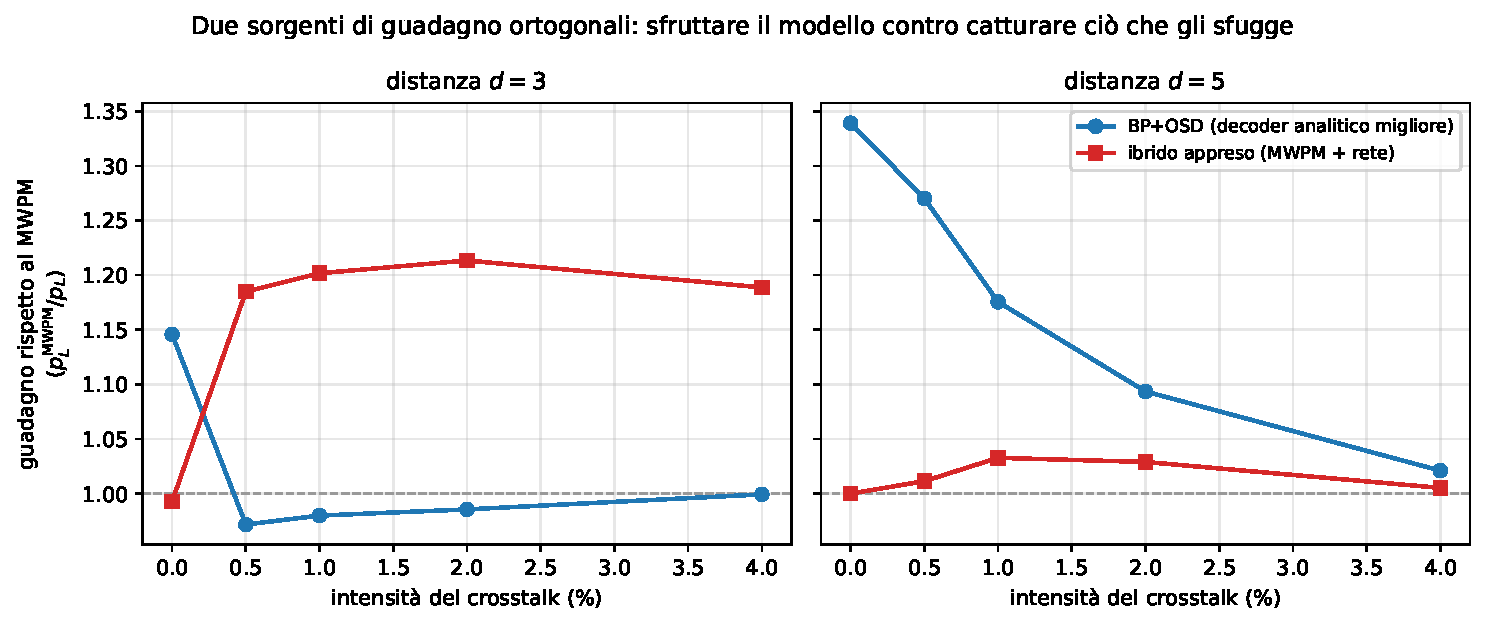
\includegraphics[width=0.95\textwidth,height=0.32\textheight,keepaspectratio]{confronto_decoder.pdf}

\caption[Ortogonalità delle due sorgenti di guadagno]{Guadagno di BP+OSD (blu) e del decoder ibrido (rosso) rispetto al \ac{MWPM}, al variare del crosstalk. La linea tratteggiata indica il guadagno unitario; i pannelli distinguono le distanze 3 e 5.}\label{fig:confronto_decoder}
\end{figure}

La Figura~\ref{fig:confronto_decoder} evidenzia il diverso andamento dei due approcci: BP+OSD perde vantaggio quando il crosstalk rende incompleto il modello di rumore, mentre il decoder ibrido recupera una parte degli errori non rappresentati. Il codice di generazione è \texttt{figure\_src/gen\_confronto\_decoder.py}.


A distanza 5 il vantaggio di BP+OSD scende monotonamente da $1.339$ a $1.021$ mentre il crosstalk aumenta; a distanza 3 esso si annulla immediatamente, e il decoder diventa lievemente \emph{peggiore} del matching. Specularmente, il guadagno dell'ibrido è nullo in assenza di crosstalk e sale fino a $1.213$. I due metodi non competono sullo stesso asse: \textbf{BP+OSD sfrutta meglio il modello che riceve, il decoder appreso cattura ciò che al modello sfugge}. Il primo rende al massimo quando il modello è corretto e si degrada man mano che diventa incompleto --- perché fidarsi più a fondo di una descrizione sbagliata è un danno, non un vantaggio; il secondo rende zero quando il modello è corretto, perché non c'è nulla da aggiungere, e cresce esattamente nella misura in cui il modello si allontana dal dispositivo.

Ne discende una conclusione più articolata di quella che l'esperimento si proponeva di verificare, e va enunciata riconoscendo entrambi i suoi lati. Da un lato l'obiezione è \textbf{in parte fondata}: a distanza 5, dove il vantaggio di partenza di BP+OSD è ampio, esso resta superiore all'ibrido in tutte le configurazioni, e adottare un decoder analitico migliore rende più che addestrare una rete. Chi disponga di un budget di ingegneria limitato dovrebbe spenderlo lì per primo, ed è una raccomandazione pratica che questa tesi non avrebbe potuto formulare senza l'esperimento. Dall'altro lato l'obiezione \textbf{non elimina il risultato}: a distanza 3 l'ibrido guadagna $18$--$21\%$ proprio dove BP+OSD perde.

Resta da chiarire che cosa significhi ``agire su assi ortogonali''. L'inferenza immediata è che i due guadagni siano \emph{sommabili}, e che costruire il residuo appreso sopra BP+OSD anziché sopra il matching debba produrre il prodotto dei due --- ossia, a distanza 5 e crosstalk $5\times10^{-3}$, un guadagno di $1.289 \times 1.010 = 1.302$. È una previsione quantitativa, e l'esperimento successivo la mette alla prova anziché darla per buona.

\subsection[E8/E10 - rumori combinati e pavimento comune]{E8 - le due sorgenti si sommano davvero? E10 - il pavimento comune}
\label{subsec:neural_pavimento}

\begin{table}[H]

\centering
\small
\begin{tabular}{ccccc c}
\toprule
$d$ & $p_{ct}$ & \textbf{BP+OSD} & \textbf{MWPM+res} & \textbf{combinato} & \textbf{prodotto previsto} \\
\midrule
3 & 0      & 1.181 & 1.079 & 1.190 & 1.274 \\
\addlinespace[0.15em]
3 & 0.005  & 0.985 & 1.192 & 1.183 & 1.173 \\
\addlinespace[0.15em]
3 & 0.01   & 0.982 & 1.205 & 1.203 & 1.183 \\
\addlinespace[0.15em]
3 & 0.02   & 0.985 & 1.211 & 1.200 & 1.193 \\
\addlinespace[0.15em]
3 & 0.04   & 0.997 & 1.184 & 1.177 & 1.180 \\
\midrule
5 & 0      & 1.180 & 1.000 & 1.180 & 1.180 \\
\addlinespace[0.15em]
5 & 0.005  & 1.289 & 1.010 & 1.289 & 1.302 \\
\addlinespace[0.15em]
5 & 0.01   & 1.196 & 1.026 & 1.200 & 1.228 \\
\addlinespace[0.15em]
5 & 0.02   & 1.093 & 1.028 & 1.104 & 1.123 \\
\addlinespace[0.15em]
5 & 0.04   & 1.024 & 1.007 & 1.024 & 1.032 \\
\bottomrule
\end{tabular}
\caption[Il residuo appreso costruito sopra BP+OSD]{Esperimento E8: guadagni $p_L^{\text{MWPM}}/p_L^{\text{metodo}}$ sugli stessi $8\times10^5$ campioni per configurazione, di cui $2\times10^5$ di test.}\label{tab:neural_e8}

\end{table}

\paragraph{La previsione e il suo esito.}
Nella Tabella~\ref{tab:neural_e8}, ``combinato'' indica il residuo appreso costruito sopra BP+OSD; ``prodotto previsto'' è il valore richiesto dall'ipotesi moltiplicativa. Il combinato non lo raggiunge quando entrambi i componenti hanno un guadagno reale, e coincide invece con il migliore dei due singoli.

L'esperimento E8 sostituisce il decoder di base del metodo ibrido descritto
nella Sezione~\ref{sec:decodifica_appresa}: il residuo appreso viene costruito
sopra BP+OSD anziché sopra il matching, e i quattro bracci --- \ac{MWPM},
BP+OSD, ciascuno con e senza residuo --- sono misurati \emph{sui medesimi
campioni}, il che rende ogni confronto appaiato ed elimina il disallineamento
fra le campagne precedenti. Le due ipotesi in gioco erano dichiarate prima
dell'esecuzione: quella \emph{moltiplicativa}, per cui il combinato approssima
il prodotto; e quella di \emph{saturazione}, per cui il residuo trova sopra
BP+OSD assai meno di quanto trovasse sopra il matching, perché una parte di ciò
che recuperava era semplicemente il costo di un decoder analitico subottimale.
La seconda è l'ipotesi sfavorevole al risultato di questa sezione, ed è quella
che i dati sostengono.



Il confronto decisivo è nelle righe in cui \emph{entrambi} i componenti guadagnano. A distanza 3 ve n'è una sola, quella senza crosstalk: il prodotto richiede $1.274$, il combinato si ferma a $1.190$, ossia esattamente il guadagno di BP+OSD da solo --- e il residuo, sopra BP+OSD e senza crosstalk, ribalta lo $0.04\%$ delle predizioni con $p = 0.58$, cioè non trova nulla. Nelle altre righe di quel blocco il ``prodotto'' è soddisfatto soltanto perché degenere: con BP+OSD a $0.98$ esso coincide per costruzione con il guadagno del residuo. A distanza 5, dove BP+OSD conserva un vantaggio ampio anche sotto crosstalk, tutte e cinque le righe sono informative e tutte e cinque smentiscono la previsione: lo scarto dal prodotto è negativo ovunque, da $-0.007$ a $-0.027$, e il residuo migliora BP+OSD in modo statisticamente significativo in \emph{una sola} configurazione su cinque, e ivi dell'uno per cento.

\begin{quote}
\emph{Il decoder combinato eguaglia sempre il migliore dei due singoli, mai il loro prodotto. Le due sorgenti di guadagno non sono sommabili: sono alternative.}
\end{quote}

\paragraph{Perché: esiste un pavimento comune.}
L'esperimento E10 individua la ragione. Sei bracci sono misurati sui medesimi campioni a distanza 3, in ordine crescente di informazione utilizzata: il decoder \emph{banale} che predice sempre l'assenza di flip logico, la rete usata \emph{da sola} senza alcun modello analitico, il \ac{MWPM}, BP+OSD, e i due residui costruiti sui due decoder analitici.

\begin{table}[H]

\centering
\footnotesize
\setlength{\tabcolsep}{4pt}
\begin{tabular}{c ccc ccc c}
\toprule
$p_{ct}$ & \textbf{banale} & \textbf{MWPM} & \textbf{BP+OSD} & \textbf{rete sola} & \textbf{MWPM+res} & \textbf{BP+OSD+res} & \textbf{disp.} \\
\midrule
0     & 0.04863 & 0.00432 & 0.00367 & 0.00431 & 0.00405 & 0.00354 & $19.4\%$ \\
\addlinespace[0.3em]
0.005 & 0.08369 & 0.03106 & 0.03195 & 0.02704 & 0.02676 & 0.02677 & $1.0\%$ \\
\addlinespace[0.3em]
0.01  & 0.11611 & 0.05928 & 0.06035 & 0.04965 & 0.04885 & 0.04982 & $2.0\%$ \\
\addlinespace[0.3em]
0.02  & 0.17464 & 0.11169 & 0.11292 & 0.09222 & 0.09108 & 0.09156 & $1.2\%$ \\
\addlinespace[0.3em]
0.04  & 0.26492 & 0.20753 & 0.20819 & 0.17565 & 0.17413 & 0.17536 & $0.9\%$ \\
\bottomrule
\end{tabular}
\caption[Sei decoder, un solo pavimento]{Esperimento E10: errore logico dei sei bracci a distanza 3, tutti sugli stessi $8\times10^5$ campioni. La colonna ``disp.'' è la dispersione relativa fra i tre bracci di fondo --- rete sola, \ac{MWPM}+residuo, BP+OSD+residuo. In presenza di crosstalk essi convergono entro il $2\%$ pur partendo da metodi radicalmente diversi; in sua assenza divergono del $19\%$ e si ordinano per qualità intrinseca del decoder.}\label{tab:neural_pavimento}

\end{table}

Il quadro si legge in due regimi, ed è la struttura stessa del risultato.

\emph{A modello corretto} (prima riga) il pavimento non esiste: i metodi si ordinano per qualità, BP+OSD davanti a tutti con $3.54\times10^{-3}$ e la rete sola ultima con $4.31\times10^{-3}$, e la dispersione fra i bracci di fondo è del $19\%$. Qui l'unica cosa che conta è quanto bene si sfrutti il modello, e il residuo appreso non ha nulla da aggiungere.

\emph{A modello strutturalmente incompleto} (le altre quattro righe) i tre bracci di fondo collassano entro lo $0.9$--$2.0\%$ l'uno dall'altro, mentre i due decoder analitici da cui provengono restano il $16$--$18\%$ sopra. Vi arriva anche la rete usata da sola, che non dispone di alcun decoder analitico: il pavimento non è dunque una proprietà del metodo di decodifica, ma \textbf{dell'informazione contenuta nella sindrome}. Sotto crosstalk ciascuno di questi metodi la estrae per intero, e incontra lo stesso limite.

L'onestà richiede una precisazione sulla parola ``coincidono''. Il test di McNemar fra la rete sola e il \ac{MWPM}+residuo dà $p = 7.8\times10^{-4}$, $8.2\times10^{-4}$ e $2.6\times10^{-3}$ ai tre livelli superiori di crosstalk: con $2\times10^{5}$ campioni di test si risolve anche uno scarto dell'uno per cento, e quelle differenze residue sono \emph{reali}. Ciò che si afferma è più debole e più preciso: i tre metodi atterrano entro l'$1$--$2\%$ l'uno dall'altro, e tale scarto è un ordine di grandezza inferiore al divario che separa tutti e tre dal decoder analitico da cui partono.

Il fallimento di E8 discende allora da E10 senza bisogno di ulteriori ipotesi: impilare i due metodi non porta sotto il pavimento, perché il pavimento non appartiene a nessuno dei due.

\paragraph{Il pavimento è del problema o del modello? (E11)}
Alla lettura appena data si può muovere un'obiezione che va presa sul serio, perché è la stessa che questa sezione muove agli altri risultati. I tre bracci che convergono contengono \emph{tutti e tre la medesima rete}, un percettrone $(128, 64)$ addestrato sugli stessi $4.8\times10^5$ campioni: che convergano potrebbe significare soltanto ``questo è quanto estrae questa rete'', e il pavimento sarebbe una proprietà del modello, non del problema. Per distinguere le due letture occorrono metodi più potenti di quel percettrone. L'esperimento E11 ne mette due alla prova, a distanza 3 e sui medesimi campioni.

Il primo è una rete con la stessa ricetta ma architettura $(512, 256, 128)$, ossia circa quaranta volte i parametri. Il secondo è il \textbf{decoder empirico a massima verosimiglianza}: per ogni sindrome osservata in addestramento si predice l'osservabile di maggioranza, con ricaduta sul \ac{MWPM} per le sindromi mai viste. Quest'ultimo non stima parametri --- memorizza --- e non ha dunque alcun limite di capacità.

\begin{table}[H]

\centering
\small
\begin{tabular}{c c ccc c}
\toprule
$p_{ct}$ & \textbf{pavimento} & \textbf{rete $40\times$} & \textbf{residuo $40\times$} & \textbf{tabella empirica} & \textbf{copertura} \\
\midrule
0.005 & 0.02688 & 0.02687 & 0.02617 & 0.02765 & $98.1\%$ \\
\addlinespace[0.3em]
0.01  & 0.04935 & 0.04920 & 0.04850 & 0.05032 & $97.4\%$ \\
\addlinespace[0.3em]
0.02  & 0.09251 & 0.09222 & 0.09169 & 0.09499 & $95.6\%$ \\
\addlinespace[0.3em]
0.04  & 0.17602 & 0.17463 & 0.17377 & 0.18324 & $91.3\%$ \\
\bottomrule
\end{tabular}
\caption[Il pavimento alla prova di modelli più potenti]{Esperimento E11, distanza 3. ``Pavimento'' è il valore di E10 ricalcolato sugli stessi campioni. ``Copertura'' è la frazione di shot di test la cui sindrome era già stata osservata in addestramento, e misura quanto la tabella empirica sia effettivamente una tabella anziché un \ac{MWPM} travestito.}\label{tab:neural_e11}

\end{table}

L'obiezione è \textbf{respinta}: la rete con quaranta volte i parametri atterra sul pavimento entro lo $0.8\%$, e la tabella empirica --- che di capacità ne ha infinita --- risulta addirittura dal $2$ al $4\%$ \emph{peggiore}. Il pavimento non è dunque il tetto dell'architettura scelta.

Sarebbe però scorretto concluderne che esso coincida con il limite informativo della sindrome, e la ragione sta nella tabella stessa. La sua copertura è alta ($91$--$98\%$) ma la sua \emph{profondità} non lo è: a crosstalk $4\times10^{-2}$ le sindromi distinte osservate sono $63\,180$ su $4.8\times10^5$ campioni di addestramento, ossia circa sette osservazioni per sindrome, e un voto di maggioranza su sette campioni è in larga parte rumore. La tabella non fallisce perché l'informazione manchi, ma perché a questa numerosità non riesce a stimarla; essa mette dunque alla prova l'ipotesi della capacità --- e la scarta --- senza stabilire alcun limite superiore informativo. Nella stessa direzione va notato che il residuo costruito sulla rete grande scende dell'$1$--$3\%$ sotto il pavimento in tutti e quattro i punti, in modo piccolo ma sistematico: il pavimento non è perfettamente duro.

L'enunciato che i dati sostengono è pertanto il seguente, e va tenuto entro questi limiti: \emph{il pavimento è robusto a un aumento di quaranta volte della capacità del modello e a un'alternativa non parametrica, e non è quindi un artefatto dell'architettura; se esso coincida con il limite informativo della sindrome resta una questione aperta, che solo una decodifica esatta a massima verosimiglianza potrebbe chiudere.}

\subsection{E5 - il decoder è trasferibile fra profili di rumore?}
\label{subsec:neural_generalizzazione}

Gli esperimenti precedenti addestrano e valutano il decoder sul \emph{medesimo} profilo di rumore. È una scelta che lascia aperta l'obiezione più concreta che si possa muovere a un decoder appreso: se il modello funzionasse soltanto sul profilo su cui è stato addestrato, andrebbe riaddestrato per ogni esemplare di \ac{QPU} e a ogni deriva di calibrazione, e il costo pratico ne annullerebbe il vantaggio. La domanda decisiva è dunque se la rete abbia appreso una \emph{regola} o le idiosincrasie di un profilo.

La verifica consiste nell'addestrare su un'intensità di rumore correlato e valutare su un'altra, senza alcun riaddestramento. Il confronto ha due termini di riferimento: il \ac{MWPM}, che non si addestra e resta quindi invariante, e la rete addestrata sullo stesso profilo di test, che rappresenta il limite superiore ottenibile conoscendo perfettamente il dominio.

\begin{table}[H]

\centering
\small
\begin{tabular}{lcccc}
\toprule
\textbf{Addestrata su} & \multicolumn{4}{c}{\textbf{Valutata su} $p_{ct}$} \\
\cmidrule(lr){2-5}
 & $5\times10^{-3}$ & $10^{-2}$ & $2\times10^{-2}$ & $4\times10^{-2}$ \\
\midrule
$5\times10^{-3}$ & \textit{0.02804} & 0.05000 & 0.09684 & 0.18749 \\
\addlinespace[0.3em]
$10^{-2}$        & \textbf{0.02800} & \textit{0.04912} & 0.09492 & 0.18140 \\
\addlinespace[0.3em]
$2\times10^{-2}$ & 0.02814 & 0.04915 & \textit{0.09286} & 0.17800 \\
\addlinespace[0.3em]
$4\times10^{-2}$ & 0.02841 & \textbf{0.04878} & 0.09312 & \textit{0.17643} \\
\midrule
\ac{MWPM} (nessun addestramento) & 0.03232 & 0.05742 & 0.11172 & 0.20853 \\
\bottomrule
\end{tabular}
\caption[Trasferibilità del decoder appreso fra profili di rumore]{Errore logico dell'ibrido al variare del profilo di addestramento e di quello di valutazione. In corsivo la diagonale (addestramento e test sullo stesso profilo), in grassetto i due casi in cui una rete \emph{trasferita} supera quella addestrata in casa. Tutte e dodici le configurazioni fuori diagonale battono comunque il \ac{MWPM}.}\label{tab:neural_trasferimento}

\end{table}

L'esito è netto: \textbf{tutte e dodici} le reti trasferite mantengono il vantaggio sul decoder analitico, e il costo del trasferimento --- il peggioramento medio rispetto alla rete addestrata sul profilo di test --- è dell'$1.6\%$. In due casi la rete trasferita risulta addirittura migliore di quella addestrata in casa, differenza che rientra nella variabilità statistica ma che conferma l'assenza di una dipendenza sistematica dal profilo di addestramento.

La regola appresa non è dunque il singolo profilo di rumore, ma qualcosa di più generale: verosimilmente la struttura delle configurazioni di sindrome che il matching interpreta male, la quale dipende dalla geometria del codice e dalla natura correlata dell'errore più che dalla sua intensità. Il risultato vale però nel perimetro provato, in cui varia soltanto l'intensità del crosstalk simulato: il trasferimento fra dispositivi reali, che differiscono anche nella struttura del rumore, resta da verificare.

% -----------------------------------------------

\section{Il Gross code nel modello code-capacity}
\label{app:gross}
\begin{onehalfspace}

Questa sezione approfondisce la Sezione~\ref{sec:finale_5_3_8} con i
controlli di costruzione, gli sweep del decoder e la spiegazione del loro
comportamento, la validazione della ricostruzione a basso rumore e i
risultati sull'intera famiglia di codici. Tutti i numeri provengono dagli
artefatti della campagna M16, in formato JSON schema~2.0 con manifest, seed e
versioni software.

\subsection{Modello, metrica e criteri fissati in anticipo}
\label{app:gross_modello}

Il modello è code-capacity: in ogni shot ciascun qubit di dato subisce un
errore $X$ con probabilità $q$, indipendentemente dagli altri, e la
sindrome è misurata senza errori in un solo ciclo. Per la struttura CSS
dei codici considerati il settore $Z$ è equivalente e non viene simulato.
La metrica è la probabilità che almeno uno dei $k$ qubit logici del blocco
fallisca; per il surface code, che protegge un qubit logico per patch, si
usano $k$ patch indipendenti e $P_{\text{blocco}} = 1-(1-p_L)^k$.

Prima degli approfondimenti sono stati fissati tre criteri di
adeguatezza, pensati per rendere il confronto statisticamente solido e
non per favorire uno dei due codici:
\begin{enumerate}
\item ogni punto del confronto deve avere almeno 100 fallimenti; in caso
  contrario si riporta una stima a bassa statistica oppure, con zero
  fallimenti su $N$ shot, il limite superiore al 95\% $3/N$;
\item dove il primo criterio è soddisfatto, l'intervallo di confidenza al
  95\% deve avere larghezza relativa entro il 20\%;
\item le varianti ragionevoli del decoder devono dare risultati
  compatibili con il riferimento; se una variante lo migliora di oltre il
  10\% con p di McNemar inferiore a 0,01, diventa il nuovo riferimento.
\end{enumerate}
Un esito è dichiarato ``migliore'' o ``peggiore'' solo con intervalli al
95\% non sovrapposti. Il modello, la metrica e i punti del confronto non
sono stati modificati dopo aver visto i risultati.

\subsection{Controlli di costruzione e distanze}
\label{app:gross_controlli}

Per ciascun codice lo script verifica $n$, $k$ e i ranghi delle matrici
di parità; per il Gross code $n = 144$, $k = 12$, rango 66 per $H_X$ e
$H_Z$ e controlli di peso 6, come nella costruzione di
riferimento~\cite{bravyi2024}. La distanza è cercata con un metodo a
insiemi d'informazione casuali: si permutano le colonne, si porta la
matrice in forma ridotta e si leggono operatori logici di peso basso,
verificandoli poi in modo indipendente. Il metodo fornisce limiti
superiori alla distanza: trovare un logico del peso pubblicato conferma
la costruzione, trovarne uno più leggero la invaliderebbe.

\begin{table}[H]

\centering
\small
\begin{tabular}{@{}lccr@{}}
\toprule
\textbf{Codice} & \textbf{Distanza attesa} & \textbf{Trovata ($X$ / $Z$)} & \textbf{Tempo} \\
\midrule
surface $d = 5, 7, 9$ & 5, 7, 9 & 5, 7, 9 & 2--26 s \\
\addlinespace[0.3em]
$[[72,12,6]]$ & 6 & 6 / 6 & 26 s \\
\addlinespace[0.3em]
$[[90,8,10]]$ & 10 & 10 / 10 & 44 s \\
\addlinespace[0.3em]
$[[108,8,10]]$ & 10 & 10 / 10 & 79 s \\
\addlinespace[0.3em]
$[[144,12,12]]$ & 12 & 12 / 12 & 228 s \\
\addlinespace[0.3em]
$[[288,12,18]]$ & 18 & 18 / 18 & 2427 s \\
\bottomrule
\end{tabular}
\caption[Distanze dei codici bivariate bicycle]{Verifica delle distanze
con 40\,000 iterazioni per settore. Per le distanze 3, 5 e 7 il surface
code è stato controllato anche per forza bruta.}\label{tab:app_gross_distanze}

\end{table}

In nessuna corsa una correzione ha violato la sindrome, e sul surface
code \ac{MWPM} e \ac{BPOSD} danno lo stesso $p_L$ entro l'incertezza a
tutte le distanze (per esempio $4{,}55\times10^{-3}$ contro
$4{,}43\times10^{-3}$ a $d = 13$, $q = 5\%$): il riferimento non è
penalizzato dal proprio decoder.

\subsection{Scelta del decoder}
\label{app:gross_decoder}

Le prime corse usavano \ac{BPOSD} con belief propagation product-sum e
poi min-sum con fattore di scala 0,625, entrambe con aggiornamento
parallelo dei messaggi. Con queste configurazioni il Gross code
risultava peggiore di 12 patch a distanza 9 per $q \le 1\%$. Poiché il
terzo criterio non era soddisfatto, sono stati eseguiti due sweep sugli
stessi shot. La Tabella~\ref{tab:app_gross_sweep} riporta le varianti
più informative del primo.

\begin{table}[H]

\centering
\small
\begin{tabular}{@{}lcccc@{}}
\toprule
\textbf{Variante} & $q = 0{,}5\%$ & $1\%$ & $2\%$ & $3\%$ \\
\midrule
rif.\ min-sum 0,625 parallelo & $9{,}3\times10^{-6}$ & $9{,}2\times10^{-5}$ & $7{,}7\times10^{-4}$ & $2{,}95\times10^{-3}$ \\
\addlinespace[0.3em]
seriale (0,625) & 0 & $5\times10^{-7}$ & $8{,}0\times10^{-5}$ & $1{,}15\times10^{-3}$ \\
\addlinespace[0.3em]
min-sum 0,5, parallelo & 0 & $5\times10^{-7}$ & $8{,}0\times10^{-5}$ & $1{,}20\times10^{-3}$ \\
\addlinespace[0.3em]
OSD-CS ordine 60 & 0 & $6\times10^{-6}$ & $1{,}3\times10^{-4}$ & $1{,}3\times10^{-3}$ \\
\addlinespace[0.3em]
1000 iterazioni & $2{,}5\times10^{-5}$ & $1{,}6\times10^{-4}$ & $8{,}9\times10^{-4}$ & $3{,}1\times10^{-3}$ \\
\addlinespace[0.3em]
product-sum & $3{,}7\times10^{-5}$ & $2{,}9\times10^{-4}$ & $1{,}7\times10^{-3}$ & $4{,}6\times10^{-3}$ \\
\bottomrule
\end{tabular}
\caption[Sweep del decoder sul Gross code]{Primo sweep: $p_L$ del
blocco su $4$, $2$, $1$ e $0{,}4$ milioni di shot, identici per tutte le
varianti. Le altre sei varianti (fattori 0,75, 0,875 e 1,0, OSD-CS di
ordine 30, OSD-E di ordine 7, BP+LSD) sono nell'artefatto dello sweep;
nessuna è migliore della schedulazione seriale.}\label{tab:app_gross_sweep}

\end{table}

La schedulazione seriale e il fattore 0,5 riducono $p_L$ di un ordine di
grandezza o più a $q = 1$--$2\%$ e di circa 2,5 volte a $q = 3\%$, con p
di McNemar compresi fra $10^{-9}$ e $10^{-150}$. Il secondo sweep, con
riferimento seriale e undici varianti attorno ad esso su 4, 2, 0,8 e 0,4
milioni di shot a $q = 1$, 2, 3 e 4\%, non ha trovato miglioramenti
superiori al 10\%: le varianti migliori, con OSD di ordine 60, guadagnano
fra il 3 e il 5\%. A $q = 1\%$ nove decoder diversi sbagliano gli stessi
cinque shot. Il decoder seriale è quindi il riferimento definitivo; la
scelta, fatta sugli stessi dati del confronto, è stata confermata su semi
indipendenti, con cui il Gross code concorda entro il 10\%.

\paragraph{Perché la schedulazione conta.} Un terzo esperimento ha
variato il fattore di scala del min-sum parallelo da 0,400 a 1,000 a
passi di 0,025, su $5\times10^5$ shot identici a $q = 2\%$ e $3\%$,
registrando per ogni fallimento se la belief propagation aveva
convergito. Nelle configurazioni peggiori l'89--98\% dei fallimenti
avviene quando la belief propagation non converge e l'OSD sceglie la
correzione sbagliata; la convergenza a una soluzione errata resta
minoritaria. Il fallimento logico si scompone quindi in
$p_L \approx P(\text{non convergenza}) \times P(\text{errore OSD}\mid\text{non convergenza})$.
Al crescere del fattore il primo termine diminuisce, ma il secondo sale
bruscamente fra 0,5 e 0,525 e arriva al 10--20\%: nei casi difficili le
probabilità che la belief propagation passa all'OSD diventano
fuorvianti. Il prodotto ha un massimo intorno a 0,7, il che spiega
l'andamento apparentemente irregolare della griglia grossolana del primo
sweep. Anche fermare la belief propagation dopo 10 iterazioni invece che
dopo 100 riduce gli errori di circa tre volte, coerentemente con questa
interpretazione. Con la schedulazione seriale la belief propagation non
converge nello 0,07\% dei casi contro lo 0,77\% del parallelo, e $p_L$
resta piatto fra i fattori 0,4 e 0,9. Il parallelo nel suo punto
migliore e il seriale raggiungono lo stesso livello, segno che quel
livello appartiene al codice più che ai decoder.

\subsection{Basso rumore: decomposizione per peso e validazione}
\label{app:gross_peso}

A $q = 0{,}5\%$ il Gross code con decoder seriale fallisce circa una volta
ogni $10^8$ shot, e una stima diretta richiederebbe circa $10^{10}$ shot.
Poiché con errori indipendenti e priore uniforme le decisioni del decoder
non dipendono da $q$, vale esattamente
\begin{equation}
p_L(q) = \sum_{w=0}^{n} \binom{n}{w} q^{w} (1-q)^{n-w} f(w),
\label{eq:app_gross_peso}
\end{equation}
dove $f(w)$ è la probabilità di fallimento con esattamente $w$ errori.
Per il Gross code i pesi da 0 a 5 sono stati enumerati in modo
esaustivo: tutte le 498\,685\,189 configurazioni sono state decodificate
senza alcun fallimento, in circa 40 minuti. Per il surface code \ac{MWPM}
corregge per costruzione ogni errore di peso non superiore a $(d-1)/2$.
I pesi successivi sono stati campionati fino a $2\times10^7$ prove o 1000
fallimenti per peso.

La ricostruzione è stata accettata solo dopo due controlli diretti
indipendenti a $q = 1\%$, con soglia di accordo del 20\%: per il Gross
code $9{,}4\times10^{-7}$ (94 fallimenti su $10^8$ shot) contro
$1{,}01\times10^{-6}$ ricostruito, scarto del 7\%; per il surface code a
distanza 13 $1{,}350\times10^{-7}$ (135 su $10^9$) contro
$1{,}357\times10^{-7}$, scarto dello 0,5\%. I residui logici più leggeri
osservati hanno peso 12, 11 e 13 per il Gross code e per il surface code
a distanza 11 e 13, pari alle rispettive distanze.

\subsection{Famiglia bivariate bicycle e distanze maggiori}
\label{app:gross_famiglia}

La Tabella~\ref{tab:app_gross_famiglia} riporta i cinque codici della
famiglia, simulati con il decoder seriale e semi nuovi fino a $10^7$
shot o 300 fallimenti per punto.

\begin{table}[H]

\centering
\small
\setlength{\tabcolsep}{3pt}
\begin{tabular}{@{}lcccccl@{}}
\toprule
\textbf{Codice} & $0{,}5\%$ & $1\%$ & $2\%$ & $3\%$ & $5\%$ & \textbf{$d$ equiv.} \\
\midrule
$[[72,12,6]]$ & $1{,}1\times10^{-4}$ & $1{,}0\times10^{-3}$ & $9{,}2\times10^{-3}$ & $3{,}3\times10^{-2}$ & $0{,}15$ & 5--7 \\
\addlinespace[0.3em]
$[[90,8,10]]$ & $10^{-7}$ (1 ev.) & $1{,}0\times10^{-5}$ & $3{,}7\times10^{-4}$ & $3{,}3\times10^{-3}$ & $4{,}2\times10^{-2}$ & 9--13 \\
\addlinespace[0.3em]
$[[108,8,10]]$ & 0 su $10^7$ & $1{,}9\times10^{-6}$ & $1{,}5\times10^{-4}$ & $1{,}7\times10^{-3}$ & $2{,}9\times10^{-2}$ & $>11$ \\
\addlinespace[0.3em]
$[[144,12,12]]$ & 0 su $10^7$ & $1{,}1\times10^{-6}$ & $8{,}2\times10^{-5}$ & $1{,}0\times10^{-3}$ & $2{,}8\times10^{-2}$ & $>13$ da 2\% \\
\addlinespace[0.3em]
$[[288,12,18]]$ & 0 su $10^7$ & 0 su $10^7$ & $10^{-7}$ (1 ev.) & $9\times10^{-6}$ & $3{,}7\times10^{-3}$ & $>13$ da 1\% \\
\bottomrule
\end{tabular}
\caption[Famiglia bivariate bicycle]{Probabilità di fallimento del
blocco da $k$ qubit logici per i cinque codici bivariate bicycle, con il
decoder seriale. L'ultima colonna indica la distanza del surface code
le cui $k$ patch hanno lo stesso fallimento del blocco.}\label{tab:app_gross_famiglia}

\end{table}

Tutti i codici con distanza almeno 10 battono le patch di surface code
che usano lo stesso numero di qubit di dato o più. A parità di $k$ e $d$,
$[[108,8,10]]$ fa circa cinque volte meglio di $[[90,8,10]]$ a
$q = 1\%$: la distanza non esaurisce la descrizione del codice. Per
estendere il confronto del codice più grande, il surface code è stato
simulato anche a distanza 15 e 17, fino a $10^8$ shot per punto, e
$[[288,12,18]]$ fino a $10^8$ shot a $q = 2\%$ e $3\%$. Da $q = 2\%$ in su
$[[288,12,18]]$ batte 12 patch fino a distanza 17, che usano 3468 qubit
di dato contro 288: $5{,}0\times10^{-8}$ contro $1{,}28\times10^{-5}$ a
$q = 2\%$ e $9{,}5\times10^{-6}$ contro $4{,}2\times10^{-4}$ a $q = 3\%$.
A $q = 1\%$ batte le patch fino a distanza 13; oltre, e a $q = 0{,}5\%$,
i fallimenti osservati non bastano a decidere.

\subsection{Limiti}
\label{app:gross_limiti}

Restano i limiti del modello: niente errori di misura né circuito di
estrazione delle sindromi, errori $X$ indipendenti, distanze verificate
come limiti superiori e nessun confronto a livello di circuito con il
surface code della Sezione~\ref{sec:finale_5_2_3} o con i risultati
pubblicati da IBM. Il confronto conta inoltre i soli qubit di dato:
includendo le ancille, il Gross code usa 288 qubit e 12 patch a distanza
13 ne usano 4044.

\end{onehalfspace}

% -----------------------------------------------

\section{Analisi di sensibilità di Shor: dettagli e verifiche}
\label{app:shor_sensibilita}
\begin{onehalfspace}

Questa sezione completa l'analisi M8/M13 della
Sezione~\ref{sec:risultati_logico} con la separazione fra livelli, il
contesto delle stime fault-tolerant e il rapporto fra metriche QEC e proxy.

\subsection{Separazione dei quattro livelli}
\label{app:shor_quattro_livelli}

\begin{table}[H]

\centering
\small
\begin{tabularx}{\textwidth}{@{}cllX@{}}
\toprule
\textbf{Livello} & \textbf{Oggetto} & \textbf{Strumento} & \textbf{Domanda} \\
\midrule
1 & Shor ideale & Qiskit Aer & limite senza rumore \\
\addlinespace[0.3em]
2 & Shor rumoroso & Aer + noise model & sensibilità agli errori fisici \\
\addlinespace[0.3em]
3 & QEC isolata & Qiskit; Stim/PyMatching & soppressione dell'errore \\
\addlinespace[0.3em]
4 & proxy per gate & Aer + canale Pauli & sensibilità a un residuo uniforme \\
\bottomrule
\end{tabularx}
\caption[Architettura a quattro livelli della parte sperimentale]{I
quattro livelli isolano domande diverse. Il quarto non è una simulazione
fault-tolerant e non riceve automaticamente i tassi aggregati del terzo.}\label{tab:quattro_livelli}

\end{table}

Una simulazione esplicita incontra una barriera dimensionale --- sostituire
ognuno dei dodici qubit di $N=15$ con un blocco codificato conduce a
centinaia di qubit --- e una strutturale: Stim è efficiente sui circuiti
stabilizer, mentre aritmetica modulare e QFT rendono Shor non-Clifford.
Aer simula il circuito generale piccolo e Stim/PyMatching caratterizza la
QEC isolata; nessuno dei due equivale a una compilazione fault-tolerant.

Il manifest M8 registra 224 CX, 302 RZ, 70 SX, 8 misure e lo SHA-256 con
prefisso \texttt{c7f4cf3b} e suffisso \texttt{a50f4ba2c}. Ogni punto aggrega 20 repliche da
4096 shot, cioè $81\,920$ misure. Il successo per misura vale uno quando
frazioni continue e controlli MCD restituiscono fattori non banali.

\subsection{Contesto delle stime fault-tolerant}
\label{app:shor_risorse}

Le stime crittografiche comprendono routing, cicli di sindrome, fabbriche
di stati magici e schedulazione; non derivano dall'estrapolazione di
$N=15$. Gidney ed Eker\aa{} stimavano circa venti milioni di qubit e otto
ore per RSA-2048~\cite{gidney2021}; lavori successivi riducono il costo
grazie ad aritmetica, codifica e preparazione delle risorse, ma sotto
assunzioni architetturali differenti.

\begin{table}[H]

\centering
\small
\begin{tabular}{>{\raggedright\arraybackslash}p{0.26\textwidth}>{\raggedright\arraybackslash}p{0.08\textwidth}>{\raggedright\arraybackslash}p{0.20\textwidth}>{\raggedright\arraybackslash}p{0.30\textwidth}}
\toprule
\textbf{Lavoro} & \textbf{Anno} & \textbf{Bersaglio} & \textbf{Qubit fisici e tempo} \\
\midrule
Gidney ed Eker\aa{}~\cite{gidney2021} & 2019 & RSA-2048 & $\sim$20 milioni, 8 ore \\
\addlinespace[0.3em]
Gidney~\cite{gidney2025} & 2025 & RSA-2048 & $<$1 milione, $<$1 settimana \\
\addlinespace[0.3em]
Pinnacle, qLDPC~\cite{pinnacle2026} & 2026 & RSA-2048 & $<$100\,000 (preprint) \\
\addlinespace[0.3em]
Cain \emph{et al.}~\cite{cain2026} & 2026 & P-256; RSA-2048 & $\sim$10\,000 atomici; P-256 in giorni con 26\,000 (preprint) \\
\bottomrule
\end{tabular}
\caption[Traiettoria delle stime di risorsa per Shor su scala crittografica]{Le
righe non sono direttamente confrontabili: cambiano codice, modello
d'errore, ciclo e criterio di successo. Le due voci 2026 sono preprint e
nessun valore discende dalle curve di questa tesi.}\label{tab:traiettoria_risorse}

\end{table}

La discesa delle stime è trainata soprattutto da correzione e
compilazione, ma resta una valutazione prospettica. La curva M8 è una
sensibilità locale e non una previsione di risorse.

\subsection{Perché le metriche QEC non entrano direttamente in M8}
\label{app:shor_metriche}

\begin{table}[H]

\centering
\small
\begin{tabular}{>{\raggedright\arraybackslash}p{0.22\textwidth}>{\raggedright\arraybackslash}p{0.38\textwidth}>{\raggedright\arraybackslash}p{0.26\textwidth}}
\toprule
\textbf{Grandezza} & \textbf{Unità/contesto} & \textbf{Inseribile direttamente in M8?} \\
\midrule
$p_L$ di M8 & Pauli non-identità dopo ogni SX/X/CX & sì, per definizione \\
\addlinespace[0.3em]
errore Steane & fallimento del protocollo protetto & no \\
\addlinespace[0.3em]
errore surface code & fallimento logico per memoria/ciclo e distanza & no \\
\addlinespace[0.3em]
guadagno decoder & differenza nel benchmark correlato & no \\
\bottomrule
\end{tabular}
\caption[Contratto tra risultati QEC e curva M8]{La conversione richiede
circuito logico, cicli, operazioni fault-tolerant e correlazioni residue.}\label{tab:decoder_su_shor}

\end{table}

Una verifica recente su 114 atomi mostra che una variante pre-compilata
di Shor su qubit logici riduce fino alla metà la distanza in variazione
totale rispetto all'esecuzione fisica; ladder CX logiche
mostrano errori due--quattro volte inferiori e un codice $[[16,4,4]]$ un
fattore otto~\cite{rines2025}. Il risultato riguarda il vantaggio del
livello logico, non una fattorizzazione scalabile e resta soggetto alla
critica di Smolin~\cite{smolin2013}. Questa evidenza conferma
solo la direzione qualitativa del proxy; non fornisce la conversione
mancante.

\end{onehalfspace}

% -----------------------------------------------

% Il testo seguente era incluso con \inputdemoted: i suoi titoli sono
% stati abbassati di un livello direttamente nel sorgente.
\section[Compilazione consapevole della struttura: un'esplorazione]{Compilazione consapevole della struttura:\\ un'esplorazione}
\label{app:compilazione}
\begin{onehalfspace}

Questa sezione esamina due verifiche esterne al confronto principale M1--M2: la sensibilit\`a alla mappatura su una topologia eterogenea (M11/M11b) e il comportamento della ricerca TOP-4 nel proxy per gate (M13). Entrambe sono analisi esplorative. Il loro scopo \`e verificare se una metrica disponibile prima dell'esecuzione o una regola disponibile dopo la misura conservino potere informativo; non dimostrare prestazioni su una QPU reale. Il Capitolo~\ref{chap:integrazione} ne riporta la sintesi.

% -----------------------------------------------
\subsection{Previsione e selezione non sono la stessa domanda}
\label{sec:app_comp_previsione}

M11 usa la snapshot offline \texttt{FakeSherbrooke} distribuita con Qiskit IBM Runtime. Le propriet\`a \texttt{target.error} sono interpretate come \emph{average gate infidelity} (AGI) complessiva e convertite in un canale depolarizzante con la stessa AGI. Il readout, esposto dalla snapshot come un solo errore medio, viene modellato simmetricamente. Le direzioni native ECR sono conservate e ogni ECR compilato deve avere una calibrazione esplicita; \texttt{rz} \`e virtuale.

Non viene aggiunto un secondo canale $T_1/T_2$. L'AGI del gate \`e gi\`a una misura complessiva della sua non idealit\`a e sommarvi il rilassamento ricavato dalla stessa snapshot produrrebbe un doppio conteggio non quantificato. Di conseguenza M11 non separa il contributo della decoerenza: studia l'eterogeneit\`a della snapshot attraverso AGI e readout.

Il punteggio di calibrazione di un circuito compilato \`e
\begin{equation}
    s = 1-\prod_{g\in C}(1-e_g),
\end{equation}
dove $e_g$ \`e l'errore target dell'istruzione fisica o della misura. Un punteggio minore indica una fedelt\`a nominale maggiore. La correlazione fra $s$ e successo risponde alla domanda \emph{predittiva}; scegliere il layout con $s$ minimo e valutarlo su dati non usati per la scelta risponde alla domanda \emph{decisionale}. Le due non vanno confuse.

% -----------------------------------------------
\subsection{M11: pilota sui layout}
\label{sec:app_comp_pilota}

Si campionano 60 sottografi connessi di 12 qubit mediante crescita casuale. Il campionamento non \`e uniforme sullo spazio dei sottografi: l'esperimento resta quindi esplorativo e le incertezze non descrivono l'intera topologia Sherbrooke. Su ciascun sottografo il circuito $N=15$, $a=7$ viene compilato in \texttt{sx/rz/x/ecr} con direzioni ECR native, livello di ottimizzazione 3 e seed 42.

Gli 8192 shot per layout sono divisi in otto batch con seed comuni. Quattro batch costituiscono la partizione di selezione e quattro l'holdout. Si confrontano due regole: layout con punteggio $s$ minimo e layout con successo massimo sulla partizione di selezione; entrambe sono valutate soltanto sull'holdout. Questo evita di chiamare ``migliore'' il massimo osservato sugli stessi dati usati per stimarne la prestazione.

\begin{table}[H]

\centering
\small
\begin{tabular}{ll}
\toprule
\textbf{Voce} & \textbf{Contratto M11} \\
\midrule
backend & snapshot offline \texttt{FakeSherbrooke}, 127 qubit \\
\addlinespace[0.3em]
layout richiesti & 60 sottografi connessi, random-growth non uniforme \\
\addlinespace[0.3em]
circuito & $N=15$, $a=7$, 8 qubit di conteggio \\
\addlinespace[0.3em]
base / ottimizzazione & \texttt{sx/rz/x/ecr}, livello 3, seed 42 \\
\addlinespace[0.3em]
campionamento & 8192 shot, 8 batch, split 4/4 \\
\addlinespace[0.3em]
inferenza & Spearman + bootstrap 2000 sui layout \\
\bottomrule
\end{tabular}
\caption[Disegno del pilota sui layout]{Contratto preregistrato di M11. La snapshot \`e riproducibile tramite hash di calibrazione; non \`e una misura live di un dispositivo al momento dell'esecuzione.}\label{tab:app_comp_pilota}

\end{table}

\begin{table}[H]

\centering
\small
\begin{tabular}{>{\raggedright\arraybackslash}p{0.30\textwidth}>{\raggedright\arraybackslash}p{0.55\textwidth}}
\toprule
\textbf{Stima} & \textbf{Interpretazione ammessa} \\
\midrule
Spearman $s$--$P_{\rm holdout}$ & associazione di rango sul campione random-growth \\
\addlinespace[0.3em]
$P_{\rm holdout}$, minimo $s$ & resa della regola basata solo sulla calibrazione \\
\addlinespace[0.3em]
$P_{\rm holdout}$, massimo train & resa di una selezione empirica su dati separati \\
\addlinespace[0.3em]
differenza holdout & confronto esplorativo tra le due regole, non oracolo globale \\
\bottomrule
\end{tabular}
\caption[Stimandi del pilota M11]{La correlazione valuta capacit\`a predittiva; il confronto holdout valuta una decisione. Nessuna riga autorizza un claim causale sull'hardware.}\label{tab:app_comp_predittori}

\end{table}

% M11_RESULTS_BEGIN
Dei 60 layout richiesti, 40 producono un modello di rumore valido. I 20
fallimenti non sono simulazioni con successo nullo: la snapshot assegna ad
almeno un gate usato un'AGI pari a 1, valore fuori dal dominio della
conversione depolarizzante adottata, e quei layout vengono pertanto esclusi.
Fra i layout validi, $P_{\rm holdout}$ varia da 0,297 a 0,516, con mediana
0,431.

La correlazione di rango tra punteggio di calibrazione e successo holdout è
$\rho_s=-0,184$, con IC bootstrap al 95\% $[-0,456;0,124]$ (2000
ricampionamenti). L'intervallo include ampiamente lo zero: sul campione
random-growth il punteggio non mostra una capacità predittiva conclusiva. Il
layout selezionato dal minimo punteggio (ID 35) ottiene
$P_{\rm holdout}=0,451$; quello selezionato dal massimo successo sulla
partizione train (ID 48) ottiene 0,516 sull'holdout. La differenza descrittiva
è quindi $+0,065$, ma non è accompagnata da un intervallo dedicato e non va
generalizzata oltre questo pilota.

La snapshot \texttt{fake\_sherbrooke} è identificata nel JSON dal proprio hash
SHA-256, il cui prefisso è \texttt{04b6a48f}.
% M11_RESULTS_END

La Figura~\ref{fig:m11_scatter} riporta la dispersione fra partizione di selezione e holdout sui 40 layout validi.

\begin{figure}[H]
\centering
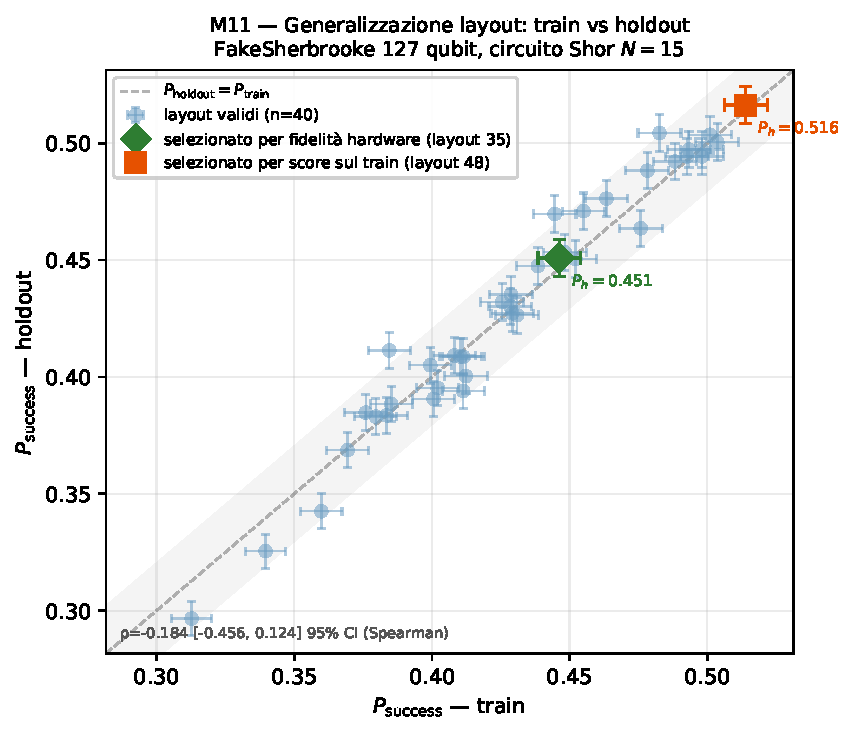
\includegraphics[width=0.72\textwidth,height=0.34\textheight,keepaspectratio]{gen_m11_scatter.pdf}

\caption[Layout M11: selezione contro holdout]{Successo in selezione e in holdout dei 40 layout M11, con barre di errore e diagonale $y=x$. Sono evidenziati i layout scelti dal punteggio di calibrazione (ID 35) e dal successo in selezione (ID 48).}\label{fig:m11_scatter}
\end{figure}

La dispersione attorno alla diagonale misura lo scarto fra successo sui dati di selezione e su dati indipendenti, motivando lo split 4/4. Gli assi \textbf{non} rappresentano la correlazione $\rho_s$ fra punteggio di calibrazione e successo holdout discussa nel testo. Il campione random-growth è non uniforme: il risultato resta osservazionale e non si generalizza all'intera topologia. Il codice di generazione è \texttt{figure\_src/gen\_m11\_scatter.py}.


\paragraph{Perch\'e la correlazione va misurata e non assunta.}
Gli strumenti di selezione del layout costruiscono un punteggio aggregando le
grandezze di calibrazione disponibili prima dell'esecuzione. I-QMapper, per
esempio, assegna a ogni layout un \emph{Layout-Quality Score} che riassume in
un solo valore gli errori di readout e di gate a due qubit del
layout~\cite{bazayeva2026}, con la stessa logica del punteggio impiegato
qui. La grandezza che tali punteggi intendono approssimare non \`e per\`o il
punteggio stesso, ma la prestazione osservata: quanto strettamente le due
siano legate \`e una domanda empirica, e su questo campione la risposta
misurata \`e debole ($\rho_s=-0,184$, con intervallo che include lo zero). Il
contributo di M11 va letto in questa direzione: non una critica a una regola
di selezione particolare --- il pilota non ne implementa nessuna di
letteratura --- ma la misura, su un campione dichiaratamente non uniforme, di
un legame che la pratica corrente tende a dare per acquisito. Un confronto
utile \`e con i metodi che ordinano i layout apprendendo da esecuzioni
passate: Hartnett e collaboratori addestrano un modello d'errore su misure di
hardware \ac{IBM} e riportano una riduzione dell'errore di selezione di
$3{,}2\times$ rispetto alla scelta casuale su un dispositivo a 16
qubit~\cite{hartnett2024}. Il contrasto \`e istruttivo e non contraddittorio:
un punteggio \emph{appreso da esecuzioni} mostra un guadagno misurato, mentre
qui \`e un punteggio \emph{derivato dalla sola calibrazione} a essere valutato,
su una snapshot e su un campione di layout non uniforme.

% -----------------------------------------------
\subsection{M11b: readout effettivo dopo il routing}
\label{sec:app_comp_ruoli}

Una seconda verifica genera variazione entro 12 sottografi. Per ciascuno vengono proposti cinque \emph{initial layout}: registri di conteggio inizialmente assegnati ai qubit con readout nominale basso o alto, layout scelto dal transpiler e due permutazioni casuali. Queste etichette non sono trattamenti. Il routing pu\`o spostare i qubit virtuali, perci\`o l'esposizione analizzata \`e l'errore medio di readout dei qubit \textbf{effettivamente misurati nel circuito finale}.

\begin{table}[H]

\centering
\small
\begin{tabular}{>{\raggedright\arraybackslash}p{0.29\textwidth}>{\raggedright\arraybackslash}p{0.61\textwidth}}
\toprule
\textbf{Voce} & \textbf{Contratto M11b} \\
\midrule
sottografi & 12, ciascuno con cinque strategie descrittive \\
\addlinespace[0.3em]
base / ottimizzazione & \texttt{sx/rz/x/ecr}, livello 2, seed 42 \\
\addlinespace[0.3em]
shot & 8192 per strategia, otto batch, holdout 50\% \\
\addlinespace[0.3em]
esposizione & readout medio sui qubit misurati dopo routing \\
\addlinespace[0.3em]
controlli & effetti fissi di sottografo, numero ECR, profondit\`a \\
\addlinespace[0.3em]
stima primaria & Spearman parziale readout--successo \\
\addlinespace[0.3em]
incertezza & cluster bootstrap sui sottografi analizzabili, 2000 ri-campionamenti \\
\bottomrule
\end{tabular}
\caption[Disegno osservazionale M11b]{L'unit\`a indipendente del bootstrap \`e il sottografo, non la singola strategia annidata.}\label{tab:app_comp_ruoli}

\end{table}

\begin{table}[H]

\centering
\small
\begin{tabular}{l>{\raggedright\arraybackslash}p{0.62\textwidth}}
\toprule
\textbf{Etichetta iniziale} & \textbf{Uso nell'analisi} \\
\midrule
\texttt{init-readout-basso} & genera una permutazione iniziale; non garantisce il readout finale \\
\addlinespace[0.3em]
\texttt{init-readout-alto} & genera variazione nella direzione opposta \\
\addlinespace[0.3em]
\texttt{transpiler} & lascia la scelta iniziale al transpiler \\
\addlinespace[0.3em]
\texttt{casuale-1/2} & due permutazioni riproducibili di confronto \\
\bottomrule
\end{tabular}
\caption[Strategie descrittive di M11b]{Le etichette sono strumenti per produrre variazione entro sottografo. Il predittore usato nel modello \`e sempre la propriet\`a osservata dopo il routing.}\label{tab:app_comp_strategie}

\end{table}

% M11B_RESULTS_BEGIN
Dei 12 sottografi richiesti, nove risultano analizzabili per tutte le cinque
strategie, per un totale di 45 osservazioni holdout. Nei tre sottografi esclusi
la conversione del modello di calibrazione incontra un'AGI pari a 1, fuori dal
dominio della parametrizzazione depolarizzante: anche in questo caso le righe
escluse non rappresentano esecuzioni con successo nullo.

Dopo la rimozione degli effetti fissi di sottografo e il controllo per numero di
ECR e profondit\`a, la correlazione parziale di Spearman fra errore medio di
readout effettivo e successo \`e $\rho_s=-0,605$. L'IC al 95\% ottenuto con 2000
ricampionamenti cluster a livello di sottografo \`e $[-0,826;-0,190]$. Nel
campione osservato, a maggiore errore di lettura corrisponde quindi un successo
inferiore anche entro sottografo; l'intervallo non include lo zero. Il risultato
resta associativo, non causale, sia per il numero ridotto di cluster sia per la
possibile presenza di propriet\`a topologiche non misurate correlate con readout,
conteggio ECR e profondit\`a.

Un'analisi indipendente ricalcola queste stime dal file dei risultati e ne
vincola il contenuto all'hash SHA-256 \texttt{1c4b5b4fad1e2289\ldots f41c196b42152215}.
% M11B_RESULTS_END

% -----------------------------------------------
\subsection{M13: TOP-4 sotto il proxy per gate}
\label{sec:app_comp_topk}

M13 usa lo stesso circuito, lo stesso manifest e la stessa definizione di $p_L$ di M8. Per ciascun punto esegue 200 repliche da 1024 shot e riusa ogni istogramma per tre endpoint: massa di successo per singola misura, TOP-1 e TOP-4. Il successo TOP-K \`e binario per replica: almeno uno dei candidati selezionati conduce ai fattori.

Un pareggio al confine del quarto posto rende la selezione non identificata. Il runner salva quindi: (i) una scelta pseudo-casuale riproducibile; (ii) un limite inferiore, vero solo quando ogni scelta ammissibile contiene un esito utile; (iii) un limite superiore, vero quando almeno una scelta ammissibile pu\`o contenerlo. Il contrasto primario fra $p_L=0$ e il massimo preregistrato usa un intervallo Newcombe; l'equivalenza richiede che l'intero intervallo cada entro $\pm0,10$. Una seconda verifica usa un inviluppo Wilson simultaneo su tutte le risoluzioni dei pareggi.

\begin{table}[H]

\centering
\small
\begin{tabular}{rcccc}
\toprule
$p_L$ & per misura & TOP-1 & TOP-4 seeded & identificato \\
\midrule
$0$ & $0{,}7512$ & $0{,}805$ & $1{,}000$ & $[1{,}000;1{,}000]$ \\
\addlinespace[0.3em]
$10^{-4}$ & $0{,}7459$ & $0{,}730$ & $1{,}000$ & $[1{,}000;1{,}000]$ \\
\addlinespace[0.3em]
$5\times10^{-4}$ & $0{,}7377$ & $0{,}690$ & $1{,}000$ & $[1{,}000;1{,}000]$ \\
\addlinespace[0.3em]
$10^{-3}$ & $0{,}7229$ & $0{,}620$ & $1{,}000$ & $[1{,}000;1{,}000]$ \\
\addlinespace[0.3em]
$1{,}7\times10^{-3}$ & $0{,}7080$ & $0{,}620$ & $1{,}000$ & $[1{,}000;1{,}000]$ \\
\addlinespace[0.3em]
$2\times10^{-3}$ & $0{,}7003$ & $0{,}650$ & $1{,}000$ & $[1{,}000;1{,}000]$ \\
\addlinespace[0.3em]
$5\times10^{-3}$ & $0{,}6396$ & $0{,}505$ & $1{,}000$ & $[1{,}000;1{,}000]$ \\
\addlinespace[0.3em]
$10^{-2}$ & $0{,}5652$ & $0{,}645$ & $1{,}000$ & $[1{,}000;1{,}000]$ \\
\addlinespace[0.3em]
$2\times10^{-2}$ & $0{,}4528$ & $0{,}695$ & $1{,}000$ & $[1{,}000;1{,}000]$ \\
\addlinespace[0.3em]
$5\times10^{-2}$ & $0{,}2979$ & $0{,}760$ & $1{,}000$ & $[1{,}000;1{,}000]$ \\
\addlinespace[0.3em]
$10^{-1}$ & $0{,}2506$ & $0{,}535$ & $0{,}915$ & $[0{,}855;0{,}940]$ \\
\addlinespace[0.3em]
$2\times10^{-1}$ & $0{,}2469$ & $0{,}245$ & $0{,}670$ & $[0{,}535;0{,}860]$ \\
\bottomrule
\end{tabular}
\caption[Endpoint preregistrati di M13]{Endpoint estratti dall'artefatto M13 schema~2 del 26 agosto 2026. La colonna ``identificato'' riporta i limiti inferiore e superiore generati dai pareggi al confine del TOP-4.}\label{tab:app_comp_topk}

\end{table}

% M13_APPENDIX_RESULTS_BEGIN
Il contrasto primario preregistrato confronta il TOP-4 seeded a $p_L=0$ con quello al massimo valore della griglia, $p_L=0,2$. La differenza stimata \`e 0,330 e l'IC Newcombe 95\% \`e $[0,266;0,398]$. La regola di equivalenza richiedeva l'intero intervallo entro $\pm0,10$; la regola di discriminazione richiedeva invece che il limite inferiore della diminuzione superasse 0,10. L'esito preregistrato \`e una diminuzione discriminante: il TOP-4 non \`e equivalente sul dominio completo della griglia.

Le analisi di sensibilit\`a confermano che la gestione dei pareggi \`e materiale. Se tutti i pareggi sono risolti nel senso pi\`u sfavorevole, la diminuzione stimata \`e 0,465 con IC $[0,395;0,534]$; nel senso pi\`u favorevole \`e 0,140 con IC $[0,095;0,195]$, non sufficiente per superare il margine con la stessa regola di discriminazione. L'inviluppo simultaneo Bonferroni-Wilson su tutte le risoluzioni ammissibili \`e $[0,059;0,553]$ e non supporta equivalenza per tutte le risoluzioni dei pareggi. Il risultato va quindi letto cos\`i: TOP-4 \`e estremamente efficace fino a $p_L=0,05$ su $N=15$, ma degrada in modo statisticamente visibile agli errori pi\`u alti della griglia.
% M13_APPENDIX_RESULTS_END

% -----------------------------------------------
% Fonti: artefatti M15/M15b schema 2 elencati in coda.
\subsection{QFT approssimata: protocolli, controlli ed esiti completi}
\label{sec:app_aqft}

Questa sezione approfondisce la Sezione~\ref{sec:qft_topologia}.
Distingue il pilota $N=15$, la compilazione strutturale $N=21$, le prove
rumorose a budget ridotto e il benchmark QPE. Sono esperimenti diversi:
la campagna principale M1--M4 resta limitata a $N=15$.

\subsubsection{Protocollo e controllo degli SWAP}

$k_{\mathrm{QPE}}$ limita la distanza fra qubit delle rotazioni
controllate nella QFT inversa finale; $k_{\mathrm{arith}}$ applica lo
stesso criterio agli addizionatori modulari di Beauregard.
Quest'ultimo non si applica al moltiplicatore specializzato per $N=15$.
Il rumore deriva da AGI e readout della snapshot \texttt{FakeSherbrooke},
con RZ virtuali e senza aggiunta separata di $T_1/T_2$. Il seed principale
è 42; i JSON registrano layout, schedule dei seed, batch, versioni e hash
della calibrazione. La scelta usa i batch di selezione e la valutazione
primaria usa batch holdout disgiunti.

Nella variante senza SWAP non basta invertire l'associazione dei bit alla
misura: poiché gli SWAP precedono la cascata di rotazioni, anche questa va
coniugata con l'inversione degli indici. Così costruiti, i bracci con e senza
SWAP del pilota $N=15$ hanno gli stessi conteggi di gate, profondità e
conteggi di successo: il transpiler assorbe già la permutazione nel layout.

\subsubsection{Pilota su \texorpdfstring{$N=15$}{N=15}}

Ogni configurazione usa 8192 shot in otto batch, quattro per selezione
e quattro per holdout. La griglia comprende tutti i gradi; le configurazioni
duplicate senza SWAP sono omesse dal riepilogo.

I risultati completi sono riportati nella Tabella~\ref{tab:finale_5_22} del Capitolo~\ref{chap:risultati}.

Il grado scelto sulla selezione è 1; il contrasto holdout è $+0.1487$,
IC Newcombe 95\% $[+0.1273;+0.1699]$, con 83 ECR risparmiate.
Il caso è favorevole perché $r=4$ produce fasi esatte in due bit:
non va generalizzato all'aritmetica per $N=21$.

\subsubsection{Struttura e prove rumorose su \texorpdfstring{$N=21$}{N=21}}

La ricognizione iniziale contiene 84 configurazioni di sola compilazione,
non 84 simulazioni rumorose. A QFT finale piena, il conteggio ECR iniziale
passa da 46\,940 per aritmetica piena a 22\,631 per
$k_{\mathrm{arith}}=1$. I circuiti ricompilati per la sensibilità
rumorosa hanno invece 49\,661 e 23\,178 ECR: conteggi ottenuti da
compilazioni differenti non vanno mescolati.

Il pilota nominale esegue soltanto il braccio troncato con 256 shot,
due batch e 128 shot holdout, ottenendo $0.2813$. Mancando il riferimento
pieno nello stesso pilota, non permette un contrasto completo.
I tre livelli successivi usano 256 shot per braccio in quattro batch,
con 128 shot holdout. Il confronto considera sempre la variante
aritmetica troncata con quella piena, anche quando la selezione
preferisce quest'ultima.

I risultati completi sono riportati nella Tabella~\ref{tab:finale_5_25} del Capitolo~\ref{chap:risultati}.

Al fattore 0.003 la selezione sceglie la QFT piena; la Tabella~\ref{tab:finale_5_25} riporta
comunque il contrasto fra troncata e piena, calcolato dai conteggi holdout
con lo stesso metodo Newcombe. Tutti e tre gli intervalli includono lo zero; nessun confronto dimostra
un vantaggio della variante troncata. Il campione ridotto limita la
discriminazione di effetti piccoli. Questi test esplorativi non
estendono a $N=21$ il confronto M1--M2.

\paragraph{Il margine a miscela è una stima condizionata.}
La stima di circa tre punti percentuali usa un modello ausiliario
\begin{equation}
 P_{\mathrm{mix}}(G,e)=P_{\mathrm{floor}}+
 (P_{\mathrm{ideal}}-P_{\mathrm{floor}})(1-e)^G,
 \label{eq:aqft_miscela}
\end{equation}
con $P_{\mathrm{ideal}}=0.4667/0.4013$ per piena/troncata e
$G=49\,661/23\,178$. Assume che ogni evento d'errore conduca al
pavimento uniforme; l'AGI usata per $e$ è un proxy e non identifica la
probabilità fisica di tale evento. Il margine dipende da questa ipotesi:
non è una misura di fedeltà, una curva rumorosa simulata o un limite
superiore dimostrato per ogni canale.

\subsubsection{Benchmark QPE: tutti i nove contrasti}

Il successo è la misura della migliore approssimazione della fase a
$n$ bit, definita da
\begin{equation}
 y_{\mathrm{target}}=\operatorname{round}(\phi 2^n)\bmod 2^n.
 \label{eq:aqft_qpe_target}
\end{equation}
Ogni grado usa 4096 shot in otto batch, quattro di selezione e quattro
holdout; il grado è scelto sulla selezione. Il confronto mantiene lo
stesso layout e la stessa schedule dei seed tra i bracci.

I risultati completi sono riportati nella Tabella~\ref{tab:finale_5_26} del Capitolo~\ref{chap:risultati}.

I nove contrasti hanno stime positive, sei intervalli escludono zero.
I risparmi ECR sono 25, 28 e 78 per $n=6,8,10$.
Il grado più favorevole fra quelli provati è 2 o 3; un layout per taglia,
una snapshot e tre fasi non dimostrano generalizzazione ad altri dispositivi.
La scelta del grado resta empirica sui batch di selezione: i conteggi e
la calibrazione possono suggerire candidati, ma questa campagna non valida
un selettore che prescinda dalle esecuzioni.

\subsection{Conclusione e limiti}
\label{sec:app_comp_conclusione}

M11 e M11b non sono un benchmark su hardware. Il simulatore e il punteggio derivano dalla stessa snapshot; questa coerenza rende il confronto controllato, ma pu\`o favorire la metrica nominale e non include deriva, crosstalk, leakage o errori coerenti. Il campionamento random-growth non \`e uniforme. M11b aumenta il controllo confrontando strategie entro lo stesso sottografo, ma resta osservazionale: readout, numero ECR e profondit\`a possono essere correlati con variabili topologiche non misurate.

M13 risponde a una domanda diversa. Una strategia TOP-4 pu\`o restare efficace anche quando la massa utile per misura \`e fortemente degradata, soprattutto nell'istanza $N=15$ con pochi picchi strutturali. Perci\`o TOP-4 deve essere riportato insieme alla metrica per misura e all'incertezza dei pareggi; da solo non misura la fedelt\`a dello stato quantistico e non pu\`o essere estrapolato a moduli maggiori.

\end{onehalfspace}


\begingroup
\setlength{\emergencystretch}{2em}
\printbibliography[heading=bibintoc, title={Bibliografia}]
\endgroup

\chapter*{Ringraziamenti}
\begin{onehalfspace}
\ifdefined\copiarelatore\else
  \providecommand{\dascrivere}[1]{{\color{gray}\small[da scrivere: #1]}}

\noindent
Dopo quasi due anni, eccoci di nuovo al momento più complicato: trovare le parole per ringraziare chi mi ha accompagnato fin qui. Spero di non dilungarmi quanto alla cena della triennale e, soprattutto, di non trasformare anche questa cena in «un funerale», come disse mio padre. Spero anche di non ripetermi troppo, ma se alcune cose le avete già sentite, è perché in questi due anni mi avete dato ancora tanti motivi per dirvele.\par

\vspace{5mm}
\dascrivere{introduzione alla famiglia, ai genitori}\par

\vspace{5mm}
\textit{A mio padre}\par
\vspace{2mm}
\dascrivere{richiamo alla triennale (il finto duro, gli Acquario, Joe Temerario) e cosa è successo in questi due anni}\par

\vspace{5mm}
\textit{A mia madre}\par
\vspace{2mm}
\dascrivere{richiamo alla triennale (lo scricciolo che stava per laurearsi, c'eri nel mio cuore) e cosa è cambiato}\par

\vspace{5mm}
\textit{A mia sorella Giulia}\par
\vspace{2mm}
\dascrivere{dalle litigate da cane e gatto al parlarsi di tutto: come è andata dopo}\par

\vspace{5mm}
\textit{A mia sorella Flavia}\par
\vspace{2mm}
\dascrivere{la principessa che cresce lontano: com'è adesso}\par

\vspace{5mm}
\textit{A Zia Enza}\par
\vspace{2mm}
\dascrivere{quella che mette ordine nel caos}\par

\vspace{5mm}
\textit{A Zia Cristina}\par
\vspace{2mm}
\dascrivere{la paura delle catastrofi e il cuore immenso}\par

\vspace{5mm}
\textit{A mia nonna Maria}\par
\vspace{2mm}
A te, presenza costante in ogni cosa fin dal mio primo giorno, anzi, da prima ancora che nascessi. A te che, nonostante la lontananza, \dascrivere{continuazione di Claudio}\par

\vfill
\begin{flushright}
    \textit{Il vostro Claudio}
\end{flushright}

\clearpage
\vspace{10mm}
\begin{center}
    \textit{A Marta}
\end{center}
\vspace{5mm}

\dascrivere{nella triennale erano cinque anni, ora sei: cosa avete vissuto in questi due anni, cosa vuoi dirle adesso}\par

\clearpage
\vspace{10mm}
\begin{center}
    \textit{Ai miei amici}
\end{center}
\vspace{5mm}

\dascrivere{introduzione agli amici, «famiglia lontano da casa»: cosa è cambiato finita la triennale}\par

\vspace{5mm}
\textit{A Omar}\par
\vspace{2mm}
Ormai non viviamo più insieme e mi manca averti in casa. Ripenso a quando sei arrivato con quel valigione enorme rosso e io mi sono chiesto: «E mo' chi è questo?». Non immaginavo che, qualche anno dopo, mi avrebbe fatto così male trovare vuota la tua stanza.\par

È successo più di una volta: sono salito in automatico, senza pensarci, come avevo fatto tante altre volte. Ho aperto la porta e tu non c'eri. Per un attimo mi ero dimenticato che non vivevamo più insieme.\par

Con te in casa mi sentivo al sicuro. Sapevo che, se avevo bisogno di parlare, di sfogarmi o anche soltanto di stare un po' in compagnia, eri a una rampa di scale da me. Con te potevo dire quello che avevo in testa senza preparare un discorso, senza paura di essere giudicato. Potevo essere me stesso, anche nelle giornate in cui facevo fatica a sopportarmi.\par

Mi manca anche il rumore delle tue ciabatte mentre studiavamo, una di quelle cose a cui allora non facevo nemmeno caso e che adesso vorrei risentire. Mi manca entrare in camera tua per dirti una stupidaggine e finire a parlare per ore. Abbiamo condiviso le feste e le follie, ma oggi mi accorgo di quanto contassero anche quei momenti normali, quando bastava sapere che eri in casa. Mi manchi, Omar.\par

Nella triennale ti avevo chiamato il mio complice, mio fratello. Ormai siamo fratelli, con due caratteri completamente diversi che, in qualche modo, si completano. Anche se, quando ci mettiamo insieme, più che completarci combiniamo un caos. E mi manca pure quello.\par

Ora siamo lontani, ma continuo a sentirti vicino. Mi hai dimostrato più di una volta che ci tieni a me e che, se ho bisogno di qualcosa, mi basta scriverti: tu ci sei, mi ascolti e mi aiuti. Questo mi dà ancora quella sicurezza che sentivo quando abitavamo insieme.\par

Grazie per essermi rimasto vicino anche da lontano. Sei ancora la persona da cui so di poter andare, anche se adesso, per raggiungerti, non basta più una rampa di scale.\par

E comunque, adesso che lavori, aspetto ancora il mio viaggio all inclusive, tutto pagato. Dopo tutte queste belle parole, direi che me lo sono meritato.\par

\vspace{5mm}
\textit{A Cosimo}\par
\vspace{2mm}
\dascrivere{la prima cassa di birra, le feste del campus, e dopo}\par

\vspace{5mm}
\textit{A Gianmaria}\par
\vspace{2mm}
\dascrivere{chi è per te, un ricordo di questi anni}\par

\vspace{5mm}
\textit{A Youssef}\par
\vspace{2mm}
\dascrivere{rum, sigari, grigliate: cosa è venuto dopo}\par

\vspace{5mm}
\textit{A Rafa}\par
\vspace{2mm}
\dascrivere{l'estate sotto lo stesso tetto e quello che è seguito}\par

\vspace{5mm}
\textit{A Noemi}\par
\vspace{2mm}
\dascrivere{dal corso di inglese a oggi}\par

\vspace{5mm}
\textit{A Francesco}\par
\vspace{2mm}
Grazie ancora per ogni discussione, ogni risata, per la fiducia che mi dai e per la pazienza con cui reggi i nostri momenti di follia. Oggi le nostre strade ci portano in posti diversi, ma quello che c'è tra noi non si misura in chilometri: ogni volta che ci ritroviamo, tutto è esattamente dove l'abbiamo lasciato.\par

Non sempre è stato facile. Ci sono stati momenti in cui il nostro rapporto ha preso dei colpi, e avrebbe potuto rovinarsi. Se non è successo, è merito della volontà di entrambi, della fiducia che abbiamo l'uno nell'altro e della forza di dirci le cose in faccia, anche quando costava. È anche per questo che oggi so quanto vale quello che c'è tra noi.\par

Ti voglio bene, Ciccio, e sono davvero contento di averti conosciuto.\par

Ora che hai la patente nautica, però, ci aspettiamo un giro in barca. Io mi prenoto già, poi a fidarmi di te al timone ci penso quando siamo lì.\par

\vspace{5mm}
\textit{A Sofia}\par
\vspace{2mm}
La tua dolcezza e la tua sincerità sono un dono raro. Con le feste a sorpresa, la tua organizzazione, i pranzi e le cene che ci prepari, riesci sempre a farci sentire tutti a casa.\par

Hai un modo tutto tuo di prenderti cura delle persone: lo fai con le cose concrete, un piatto pronto, una sorpresa pensata nei dettagli, e lo fai senza mai farlo pesare. Grazie, Sofia, perché trasformi in casa ogni posto in cui siamo insieme.\par

Ti voglio un bene immenso. E la prossima volta che ci ritroviamo a tavola, tu cucini e io porto il dolce. Anche se, lo sappiamo, la più dolce resti sempre tu.\par

\vspace{5mm}
\dascrivere{chiusura agli amici}\par

\vfill
\begin{flushright}
    \textit{Claudio Dragotta}\\
    \textit{Roma, \the\year}
\end{flushright}

\clearpage

\fi
\ifdefined\copiarelatore\else
\vspace{5mm}
\begin{center}
    \textit{Al Professore}
\end{center}
\vspace{5mm}
\fi

Al \textbf{Prof. Floriano Caprio} va un grazie che non riguarda soltanto questa tesi.

Mi ha colpito fin dalle prime lezioni e, con il tempo, quella prima impressione è diventata stima e affetto. Durante questo lavoro ho trovato in lui una disponibilità che non ho mai dato per scontata e che non è mai venuta meno.

Mi ha fatto sentire il suo affetto sincero e quanto tenesse davvero alla persona dietro queste pagine. Più di una volta mi ha detto che, quando si arrabbiava, era perché mi trattava come un figlio. Mi ha raccontato di aver commesso anche lui alcuni degli errori che vedeva in me, e di volermi aiutare a evitarli. Quelle parole mi sono rimaste dentro, perché mi hanno fatto capire quanto ci fosse di personale nella cura con cui mi seguiva. Oggi, nei suoi richiami, riconosco anche questo: il desiderio di condividere ciò che ha imparato, per aiutarmi a crescere e a trovare la mia strada.

Grazie, Professore, per la pazienza, per la fiducia e per esserci stato anche quando c'era bisogno di una parola più severa. Grazie per aver visto in me qualcosa che forse io non riesco ancora a vedere e che spero un giorno di riuscire a riconoscere. Grazie per avere creduto in me quando io facevo fatica a farlo.

Mi auguro di cuore che la fine di questa tesi non segni la fine del nostro percorso insieme, ma che le nostre strade continuino a incrociarsi. Di questo lavoro porto con me molto più di quello che è scritto in queste pagine.

Grazie, Professore Floriano.


\vspace{1cm}
\begin{flushright}
\textit{Claudio Dragotta} \\
\textit{Roma, \the\year}
\end{flushright}
\end{onehalfspace}


\end{document}
